\documentclass[9pt,a4paper,]{extarticle}

\usepackage{f1000_styles}

\usepackage[pdfborder={0 0 0}]{hyperref}

\usepackage[numbers]{natbib}
\bibliographystyle{unsrtnat}


%% maxwidth is the original width if it is less than linewidth
%% otherwise use linewidth (to make sure the graphics do not exceed the margin)
\makeatletter
\def\maxwidth{ %
  \ifdim\Gin@nat@width>\linewidth
    \linewidth
  \else
    \Gin@nat@width
  \fi
}
\makeatother

\usepackage{color}
\usepackage{fancyvrb}
\newcommand{\VerbBar}{|}
\newcommand{\VERB}{\Verb[commandchars=\\\{\}]}
\DefineVerbatimEnvironment{Highlighting}{Verbatim}{commandchars=\\\{\}}
% Add ',fontsize=\small' for more characters per line
\usepackage{framed}
\definecolor{shadecolor}{RGB}{248,248,248}
\newenvironment{Shaded}{\begin{snugshade}}{\end{snugshade}}
\newcommand{\AlertTok}[1]{\textcolor[rgb]{0.94,0.16,0.16}{#1}}
\newcommand{\AnnotationTok}[1]{\textcolor[rgb]{0.56,0.35,0.01}{\textbf{\textit{#1}}}}
\newcommand{\AttributeTok}[1]{\textcolor[rgb]{0.13,0.29,0.53}{#1}}
\newcommand{\BaseNTok}[1]{\textcolor[rgb]{0.00,0.00,0.81}{#1}}
\newcommand{\BuiltInTok}[1]{#1}
\newcommand{\CharTok}[1]{\textcolor[rgb]{0.31,0.60,0.02}{#1}}
\newcommand{\CommentTok}[1]{\textcolor[rgb]{0.56,0.35,0.01}{\textit{#1}}}
\newcommand{\CommentVarTok}[1]{\textcolor[rgb]{0.56,0.35,0.01}{\textbf{\textit{#1}}}}
\newcommand{\ConstantTok}[1]{\textcolor[rgb]{0.56,0.35,0.01}{#1}}
\newcommand{\ControlFlowTok}[1]{\textcolor[rgb]{0.13,0.29,0.53}{\textbf{#1}}}
\newcommand{\DataTypeTok}[1]{\textcolor[rgb]{0.13,0.29,0.53}{#1}}
\newcommand{\DecValTok}[1]{\textcolor[rgb]{0.00,0.00,0.81}{#1}}
\newcommand{\DocumentationTok}[1]{\textcolor[rgb]{0.56,0.35,0.01}{\textbf{\textit{#1}}}}
\newcommand{\ErrorTok}[1]{\textcolor[rgb]{0.64,0.00,0.00}{\textbf{#1}}}
\newcommand{\ExtensionTok}[1]{#1}
\newcommand{\FloatTok}[1]{\textcolor[rgb]{0.00,0.00,0.81}{#1}}
\newcommand{\FunctionTok}[1]{\textcolor[rgb]{0.13,0.29,0.53}{\textbf{#1}}}
\newcommand{\ImportTok}[1]{#1}
\newcommand{\InformationTok}[1]{\textcolor[rgb]{0.56,0.35,0.01}{\textbf{\textit{#1}}}}
\newcommand{\KeywordTok}[1]{\textcolor[rgb]{0.13,0.29,0.53}{\textbf{#1}}}
\newcommand{\NormalTok}[1]{#1}
\newcommand{\OperatorTok}[1]{\textcolor[rgb]{0.81,0.36,0.00}{\textbf{#1}}}
\newcommand{\OtherTok}[1]{\textcolor[rgb]{0.56,0.35,0.01}{#1}}
\newcommand{\PreprocessorTok}[1]{\textcolor[rgb]{0.56,0.35,0.01}{\textit{#1}}}
\newcommand{\RegionMarkerTok}[1]{#1}
\newcommand{\SpecialCharTok}[1]{\textcolor[rgb]{0.81,0.36,0.00}{\textbf{#1}}}
\newcommand{\SpecialStringTok}[1]{\textcolor[rgb]{0.31,0.60,0.02}{#1}}
\newcommand{\StringTok}[1]{\textcolor[rgb]{0.31,0.60,0.02}{#1}}
\newcommand{\VariableTok}[1]{\textcolor[rgb]{0.00,0.00,0.00}{#1}}
\newcommand{\VerbatimStringTok}[1]{\textcolor[rgb]{0.31,0.60,0.02}{#1}}
\newcommand{\WarningTok}[1]{\textcolor[rgb]{0.56,0.35,0.01}{\textbf{\textit{#1}}}}

% disable code chunks background
%\renewenvironment{Shaded}{}{}

% disable section numbers
\setcounter{secnumdepth}{0}

%% added by MLS, this is not in the F1000 style by default %%

\hypersetup{unicode=true,
            pdftitle={A Bioconductor workflow for processing, evaluating, and interpreting expression proteomics data},
            pdfkeywords={Bioconductor, QFeatures, proteomics, shotgun proteomics, bottom-up proteomics,
differential expression, mass spectrometry, quality control, data processing,
limma},
            pdfborder={0 0 0},
            breaklinks=true}

%% End added by MLS %%

\setlength{\parindent}{0pt}
\setlength{\parskip}{6pt plus 2pt minus 1pt}



\begin{document}
\pagestyle{front}

\title{A Bioconductor workflow for processing, evaluating, and interpreting expression proteomics data}

\author[1]{Charlotte Hutchings}
\author[1]{Charlotte S. Dawson}
\author[2]{Thomas Krueger}
\author[1]{Kathryn S. Lilley}
\author[1]{Lisa M. Breckels}
\affil[1]{Cambridge Centre for Proteomics, Department of Biochemistry, University of Cambridge, UK}
\affil[2]{Department of Biochemistry, University of Cambridge, UK}

\maketitle
\thispagestyle{front}

\begin{abstract}
\hfill\break
abundances within a system. In turn, differential expression analysis can be
used to investigate changes in protein abundance upon perturbation to such a
system.

interpretation of quantitative mass spectrometry-based expression proteomics
data. This workflow utilizes open-source R software packages from the
Bioconductor project and guides users end-to-end and step-by-step through every
stage of the analyses. As a use-case we generated expression proteomics data
from HEK293 cells with and without a treatment. Of note, the experiment included
cellular proteins labelled using tandem mass tag (TMT) technology and secreted
proteins quantified using label-free quantitation (LFQ).

on data import, pre-processing and quality control. This is done individually
for TMT and LFQ datasets. The application of statistical differential
expression analysis is demonstrated, followed by interpretation via gene
ontology enrichment analysis.

interpretation of expression proteomics is presented. The workflow is a
valuable resource for the proteomics community and specifically beginners who
are at least familiar with R who wish to understand and make data-driven
decisions with regards to their analyses.
\textbf{Background:} Expression proteomics involves the global evaluation of protein
\textbf{Methods:} Here, we provide a workflow for the processing, analysis and
\textbf{Results:} The workflow explains the software infrastructure before focusing
\textbf{Conclusions:} A comprehensive workflow for the processing, analysis and
\end{abstract}

\section*{Keywords}
Bioconductor, QFeatures, proteomics, shotgun proteomics, bottom-up proteomics,
differential expression, mass spectrometry, quality control, data processing,
limma


\clearpage
\pagestyle{main}

\textbf{R version}: R version 4.4.0 (2024-04-24)

\textbf{Bioconductor version}: 3.19

\section{Introduction}\label{introduction}

Proteins are responsible for carrying out a multitude of biological tasks,
implementing cellular functionality and determining phenotype. Mass spectrometry
(MS)-based expression proteomics allows protein abundance to be quantified and
compared between samples. In turn, differential protein abundance can be used to
explore how biological systems respond to a perturbation. Many research groups
have applied such methodologies to understand mechanisms of disease, elucidate
cellular responses to external stimuli, and discover diagnostic biomarkers (see
\citep{PinaJimnez2021, AmiriDashatan2021, Anitua2018} for recent examples). As the
potential of proteomics continues to be realized, there is a clear need for
resources demonstrating how to deal with expression proteomics data in a robust
and standardized manner.

The data generated during an expression proteomics experiment are complex, and
unfortunately there is no one-size-fits-all method for the processing and analysis
of such data. The reason for this is two-fold. Firstly, there are a wide range
of experimental methods that can be used to generate expression proteomics data.
Researchers can analyze full-length proteins (top-down proteomics) or complete
an enzymatic digestion and analyze the resulting peptides. This proteolytic
digestion can be either partial (middle-down proteomics) or complete (bottom-up
proteomics). The latter approach is most commonly used as peptides have a more
favourable ionization capacity, predictable fragmentation patterns, and can be
separated via reversed phase liquid chromatography, ultimately making them more
compatible with MS \citep{Dupree2020}. Within bottom-up proteomics, the relative
quantitation of peptides can be determined using one of two approaches: (1)
label-free or (2) label-based quantitation. Moreover, the latter can be
implemented with a number of different peptide labelling chemistries, for example,
using tandem mass tag (TMT), stable-isotope labelling by amino acids in cell
culture (SILAC), isobaric tags for relative and absolute quantitation (iTRAQ),
among others \citep{Obermaier2015}. MS analysis can also be used in either data-dependent
or data-independent acquisition (DDA or DIA) mode \citep{FernndezCosta2020, Hu2016}.
Although all of these experimental methods typically result in a similar output,
a matrix of quantitative values, the data are different and must be treated as such.
Secondly, data processing is dependent upon the experimental goal and biological
question being asked.

Here, we provide a step-by-step workflow for processing, analysing and
interpreting expression proteomics data derived from a bottom-up experiment
using DDA and either LFQ or TMT label-based peptide quantitation. We outline how
to process the data starting from a peptide spectrum match (PSM)- or peptide-level
\texttt{.txt} file. Such files are the outputs of most major third party search
software (e.g., Proteome Discoverer, MaxQuant, FragPipe). We begin with data
import and then guide users through the stages of data processing including data
cleaning, quality control filtering, management of missing values, imputation,
and aggregation to protein-level. Finally, we finish with how to discover
differentially abundant proteins and carry out biological interpretation of the
resulting data. The latter will be achieved through the application of gene
ontology (GO) enrichment analysis. Hence, users can expect to generate lists of
proteins that are significantly up- or downregulated in their system of interest,
as well as the GO terms that are significantly over-represented in these proteins.

Using the R statistical programming environment \citep{Rstat} we make use of several
state-of-the-art packages from the open-source, open-development Bioconductor
project \citep{Huber2015} to analyze use-case expression proteomics datasets
\citep{HutchingsData} from both LFQ and label-based technologies.

\subsection{Package installation}\label{package-installation}

In this workflow we make use of open-source software from the
\href{https://www.r-project.org}{R} \href{https://bioconductor.org}{Bioconductor}
\citep{Huber2015} project. The \href{https://bioconductor.org}{Bioconductor initiative}
provides \href{https://www.r-project.org}{R} software packages dedicated
to the processing of high-throughput complex biological data. Packages are
open-source, well-documented and benefit from an active community of developers.
We recommend users to download the
\href{https://posit.co/download/rstudio-desktop/}{RStudio} integrated development
environment (IDE) which provides a graphical interface to
\href{https://www.r-project.org}{R} programming language.

Detailed instructions for the installation of Bioconductor packages are
documented on the \href{http://bioconductor.org/install/}{Bioconductor Installation page}.
The main packages required for this workflow are installed using the code below.
Additional packages required for downstream statistics and interpretation are
installed as required.

\begin{Shaded}
\begin{Highlighting}[]
\ControlFlowTok{if}\NormalTok{ (}\SpecialCharTok{!}\FunctionTok{require}\NormalTok{(}\StringTok{"BiocManager"}\NormalTok{, }\AttributeTok{quietly =} \ConstantTok{TRUE}\NormalTok{)) \{}
  \FunctionTok{install.packages}\NormalTok{(}\StringTok{"BiocManager"}\NormalTok{)}
\NormalTok{\}}

\NormalTok{BiocManager}\SpecialCharTok{::}\FunctionTok{install}\NormalTok{(}\FunctionTok{c}\NormalTok{(}\StringTok{"QFeatures"}\NormalTok{,}
                       \StringTok{"ggplot2"}\NormalTok{,}
                       \StringTok{"stringr"}\NormalTok{,}
                       \StringTok{"NormalyzerDE"}\NormalTok{,}
                       \StringTok{"corrplot"}\NormalTok{,}
                       \StringTok{"Biostrings"}\NormalTok{,}
                       \StringTok{"limma"}\NormalTok{,}
                       \StringTok{"impute"}\NormalTok{,}
                       \StringTok{"dplyr"}\NormalTok{,}
                       \StringTok{"tibble"}\NormalTok{,}
                       \StringTok{"org.Hs.eg.db"}\NormalTok{,}
                       \StringTok{"clusterProfiler"}\NormalTok{,}
                       \StringTok{"enrichplot"}\NormalTok{))}
\end{Highlighting}
\end{Shaded}

After installation, each package must be loaded before it can be used in the R
session. This is achieved via the \texttt{library} function. For example, to load the
\texttt{QFeatures} package one would type \texttt{library("QFeatures")} after installation.
Here we load all packages included in this workflow.

\begin{Shaded}
\begin{Highlighting}[]
\FunctionTok{library}\NormalTok{(}\StringTok{"QFeatures"}\NormalTok{)}
\FunctionTok{library}\NormalTok{(}\StringTok{"ggplot2"}\NormalTok{)}
\FunctionTok{library}\NormalTok{(}\StringTok{"stringr"}\NormalTok{)}
\FunctionTok{library}\NormalTok{(}\StringTok{"dplyr"}\NormalTok{)}
\FunctionTok{library}\NormalTok{(}\StringTok{"tibble"}\NormalTok{)}
\FunctionTok{library}\NormalTok{(}\StringTok{"NormalyzerDE"}\NormalTok{)}
\FunctionTok{library}\NormalTok{(}\StringTok{"corrplot"}\NormalTok{)}
\FunctionTok{library}\NormalTok{(}\StringTok{"Biostrings"}\NormalTok{)}
\FunctionTok{library}\NormalTok{(}\StringTok{"limma"}\NormalTok{)}
\FunctionTok{library}\NormalTok{(}\StringTok{"org.Hs.eg.db"}\NormalTok{)}
\FunctionTok{library}\NormalTok{(}\StringTok{"clusterProfiler"}\NormalTok{)}
\FunctionTok{library}\NormalTok{(}\StringTok{"enrichplot"}\NormalTok{)}
\end{Highlighting}
\end{Shaded}

\section{Methods}\label{methods}

\subsection{The use-case: exploring changes in protein abundance in HEK293 cells upon perturbation}\label{the-use-case-exploring-changes-in-protein-abundance-in-hek293-cells-upon-perturbation}

As a use-case, we analyze two quantitative proteomics datasets derived from a
single experiment. The aim of the experiment was to reveal the differential
abundance of proteins in HEK293 cells upon a particular treatment, the exact
details of which are anonymized for the purpose of this workflow. An outline of
the experimental method is provided in Figure \ref{fig:experimental-method}.

Briefly, HEK293 cells were either (i) left untreated, or (ii) provided with the
treatment of interest. These two conditions are referred to as `control' and
`treated', respectively. Each condition was evaluated in triplicate. At 96-
hours post-treatment, samples were collected and separated into cell pellet and
supernatant fractions containing cellular and secreted proteins, respectively.
Both fractions were denatured, alkylated and digested to peptides using trypsin.

The supernatant fractions were de-salted and analysed over a two-hour gradient
in an Orbitrap Fusion\textsuperscript{TM} Lumos\textsuperscript{TM} Tribrid\textsuperscript{TM} mass spectrometer coupled to an
UltiMate\textsuperscript{TM} 3000 HPLC system (Thermo Fisher Scientific). LFQ was achieved at the
MS1 level based on signal intensities. Cell pellet fractions were labelled using
TMT technology before being pooled and subjected to high pH reversed-phase peptide
fractionation giving a total of 8 fractions. As before, each fraction was
analysed over a two-hour gradient in an Orbitrap Fusion\textsuperscript{TM} Lumos\textsuperscript{TM} Tribrid\textsuperscript{TM}
mass spectrometer coupled to an UltiMate\textsuperscript{TM} 3000 HPLC system (Thermo Fisher
Scientific). To improve the accuracy of the quantitation of TMT-labelled peptides,
synchronous precursor selection (SPS)-MS3 data acquisition was employed
\citep{McAlister2014, Ting2011}. Of note, TMT labelling of cellular proteins was
achieved using a single TMT6plex. Hence, this workflow will not include guidance
on multi-batch TMT effects or the use of internal reference scaling. For more
information about the use of multiple TMTplexes users are directed to \citep{Plubell2017, Brenes2019}.

\begin{figure}

{\centering 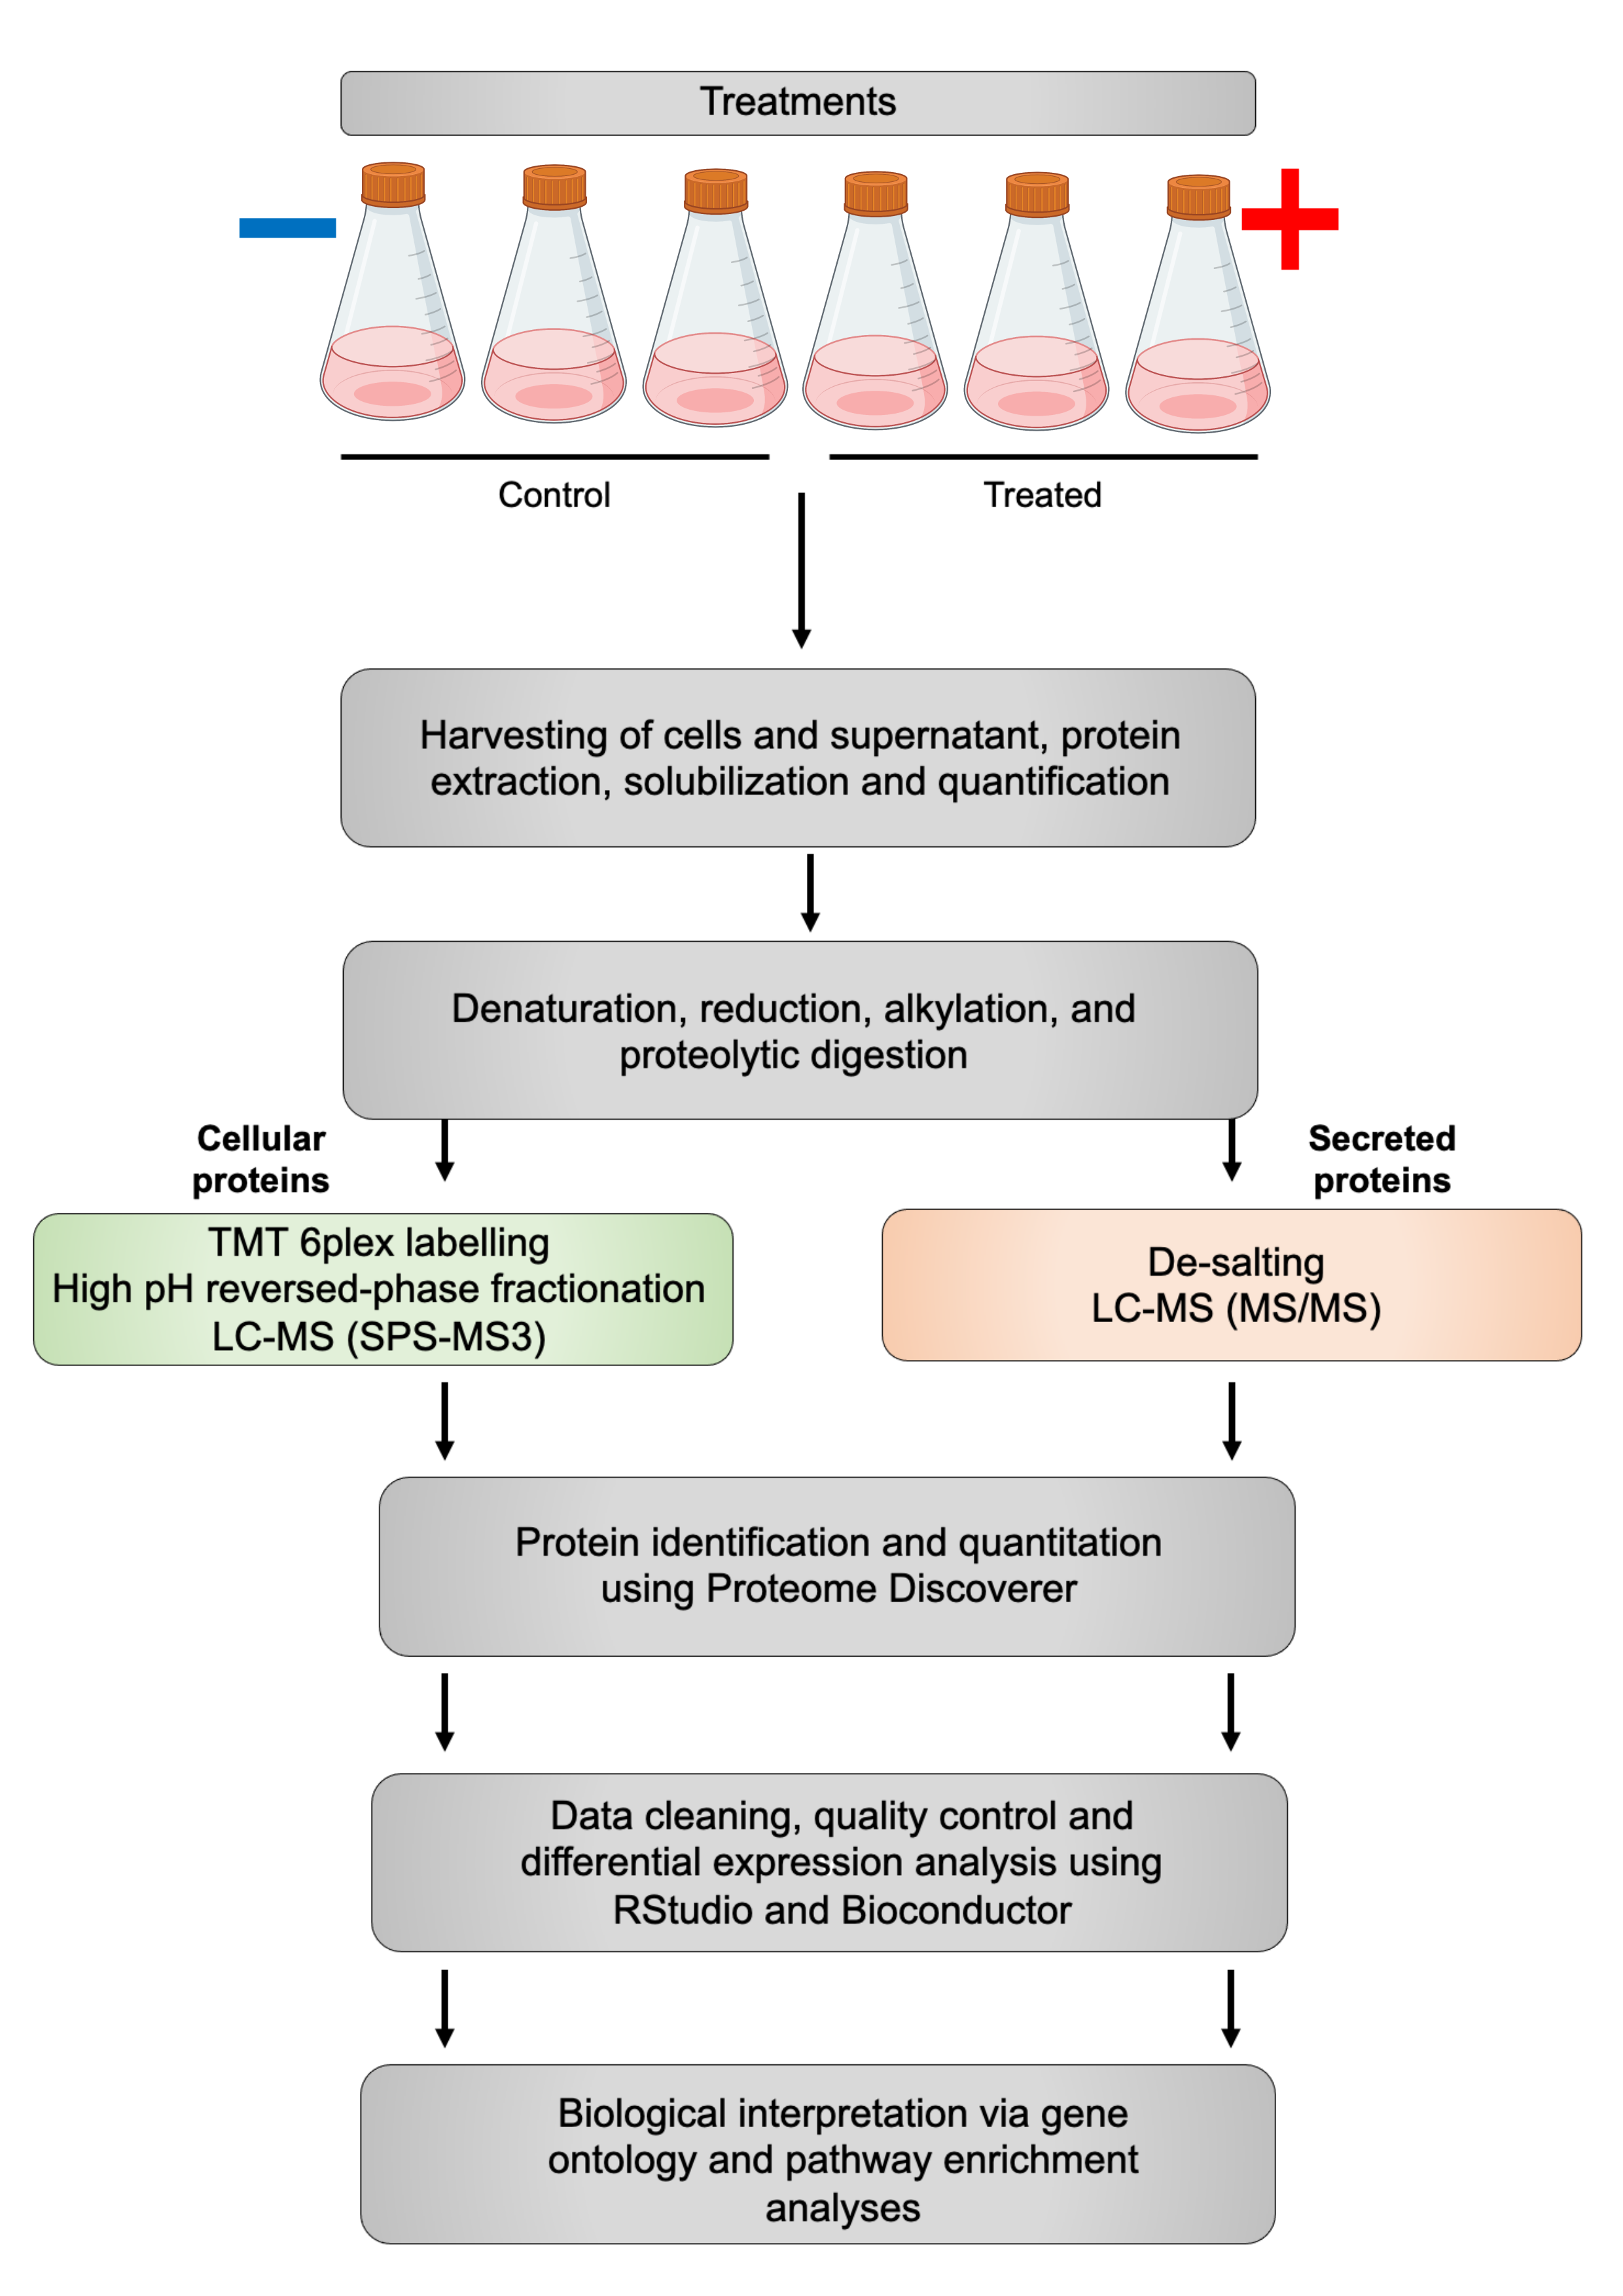
\includegraphics[width=1\linewidth]{Images/experimental-method} 

}

\caption{A schematic summary of the experimental protocol used to generate the use-case data.}\label{fig:experimental-method}
\end{figure}

The cell pellet and supernatant datasets were handled independently and we take
advantage of this to discuss the processing of TMT-labelled and LFQ proteomics
data. In both cases, the raw MS data were processed using Proteome Discoverer
v2.5 (Thermo Fisher Scientific). As a result, this workflow uses the specific
columns and files output by Proteome Discoverer. Nevertheless, most third party
software output similar data structures and this workflow can be adapted. As an
example, information on how to adapt this workflow for data processed by MaxQuant
is provided in the \href{https://github.com/CambridgeCentreForProteomics/f1000_expression_proteomics}{appendix}.
While the focus in the workflow presented below is differential protein expression
analysis, the data processing and quality control steps described here are
applicable to any TMT or LFQ proteomics dataset. Importantly, however, the
experimental aim will influence data-guided decisions and the considerations
discussed here likely differ from those of spatial proteomics, for example.

\subsection{Downloading the data}\label{downloading-the-data}

The files required for this workflow can be found deposited to the ProteomeXchange
Consortium via the PRIDE \citep{PerezRiverol2021, Deutsch2022} partner repository
with the dataset identifier PXD041794, Zenodo at \url{http://doi.org/10.5281/zenodo.11196770}
and at the Github repository \url{https://github.com/CambridgeCentreForProteomics/f1000_expression_proteomics/}.
Users are advised to download these files into their current working directory.
In R the \texttt{setwd} function can be used to specify a working directory, or if
using RStudio one can use the Session -\textgreater{} Set Working Directory menu.

\subsection{\texorpdfstring{The infrastructure: \texttt{QFeatures} and \texttt{SummarizedExperiment}s}{The infrastructure: QFeatures and SummarizedExperiments}}\label{the-infrastructure-qfeatures-and-summarizedexperiments}

To be able to conveniently track each step of this workflow, users should make
use of the Quantitative features for mass spectrometry package, or
\href{https://www.bioconductor.org/packages/release/bioc/html/QFeatures.html}{\texttt{QFeatures}, Bioconductor package}
\citep{QFeat}. Prior to utilizing the \texttt{QFeatures} infrastructure, it is first necessary to
understand the structure of a \href{https://bioconductor.org/packages/release/bioc/html/SummarizedExperiment.html}{\texttt{SummarizedExperiment}}
\citep{SumExp} object as \texttt{QFeatures} objects are based on the \texttt{SummarizedExperiment}
class. A \texttt{SummarizedExperiment}, often referred to as an SE, is a data container
and S4 object comprised of three components: (1) the \texttt{colData} (column data)
containing sample metadata, (2) the \texttt{rowData} containing data features, and (3)
the \texttt{assay} storing quantitation data, as illustrated in Figure
\ref{fig:summarized-experiment}. The sample metadata includes annotations such
as condition and replicate, and can be accessed using the \texttt{colData} function.
Data features, accessed via the \texttt{rowData} function, represent information
derived from the identification search. Examples include peptide sequence,
master protein accession, and confidence scores. Finally, quantitative data is
stored in the \texttt{assay} slot. These three independent data structures are neatly
stored within a single \texttt{SummarizedExperiment} object.



\begin{figure}

{\centering 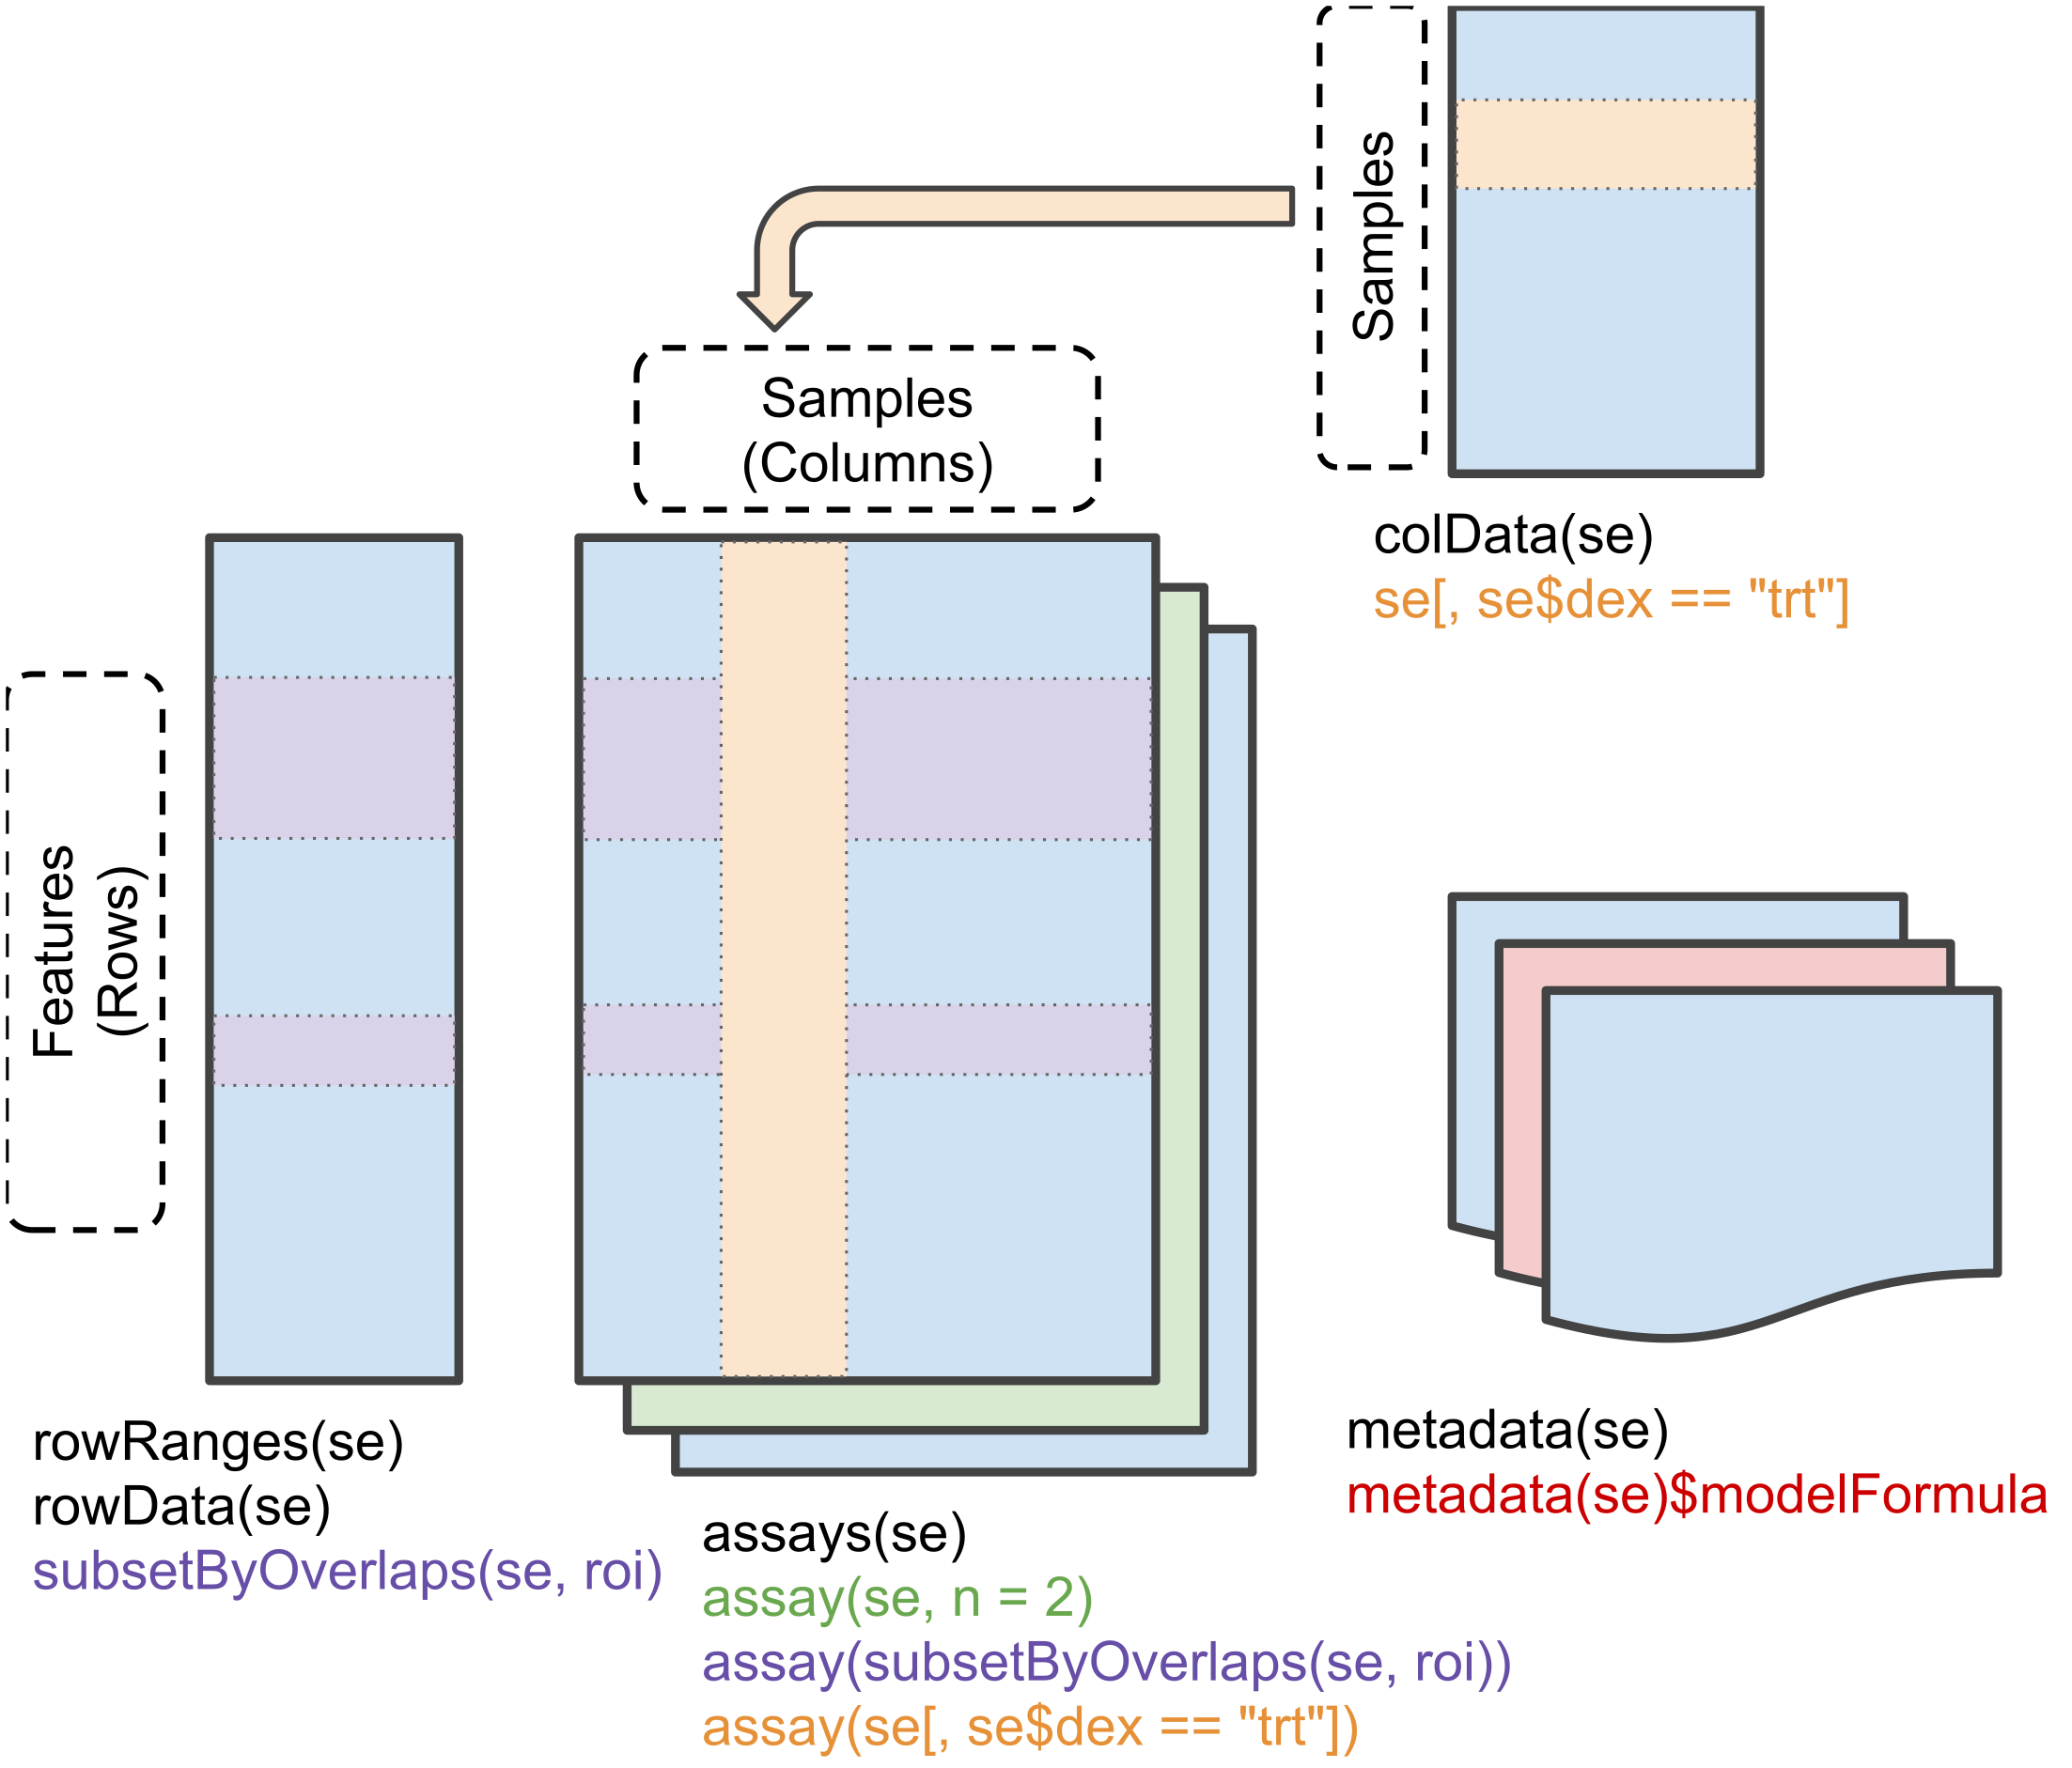
\includegraphics[width=1\linewidth]{Images/summarized-experiment} 

}

\caption{A graphic representation of the SummarizedExperiment (SE) object structure. Figure reproduced from the SummarizedExperiment package \citep{SumExp} vignette with permission.}\label{fig:summarized-experiment}
\end{figure}

A \texttt{QFeatures} object holds each level of quantitative proteomics data, namely
(but not limited to) the PSM, peptide and protein-level data. Each level of the
data is stored as its own \texttt{SummarizedExperiment} within a single \texttt{QFeatures}
object. The lowest level data e.g.~PSM, is first imported into a \texttt{QFeatures}
object before aggregating upward towards protein-level (Figure
\ref{fig:qfeatures}). During this process of aggregation, \texttt{QFeatures} maintains
the hierarchical links between quantitative levels whilst allowing easy access
to all data levels for individual proteins of interest. This key aspect of
\texttt{QFeatures} will be exemplified throughout this workflow. Additional guidance on
the use of \texttt{QFeatures} can be found in \citep{QFeat}. For visualization of the data,
all plots are generated using standard \texttt{ggplot} functionality, but could equally
be produced using base R.



\begin{figure}

{\centering 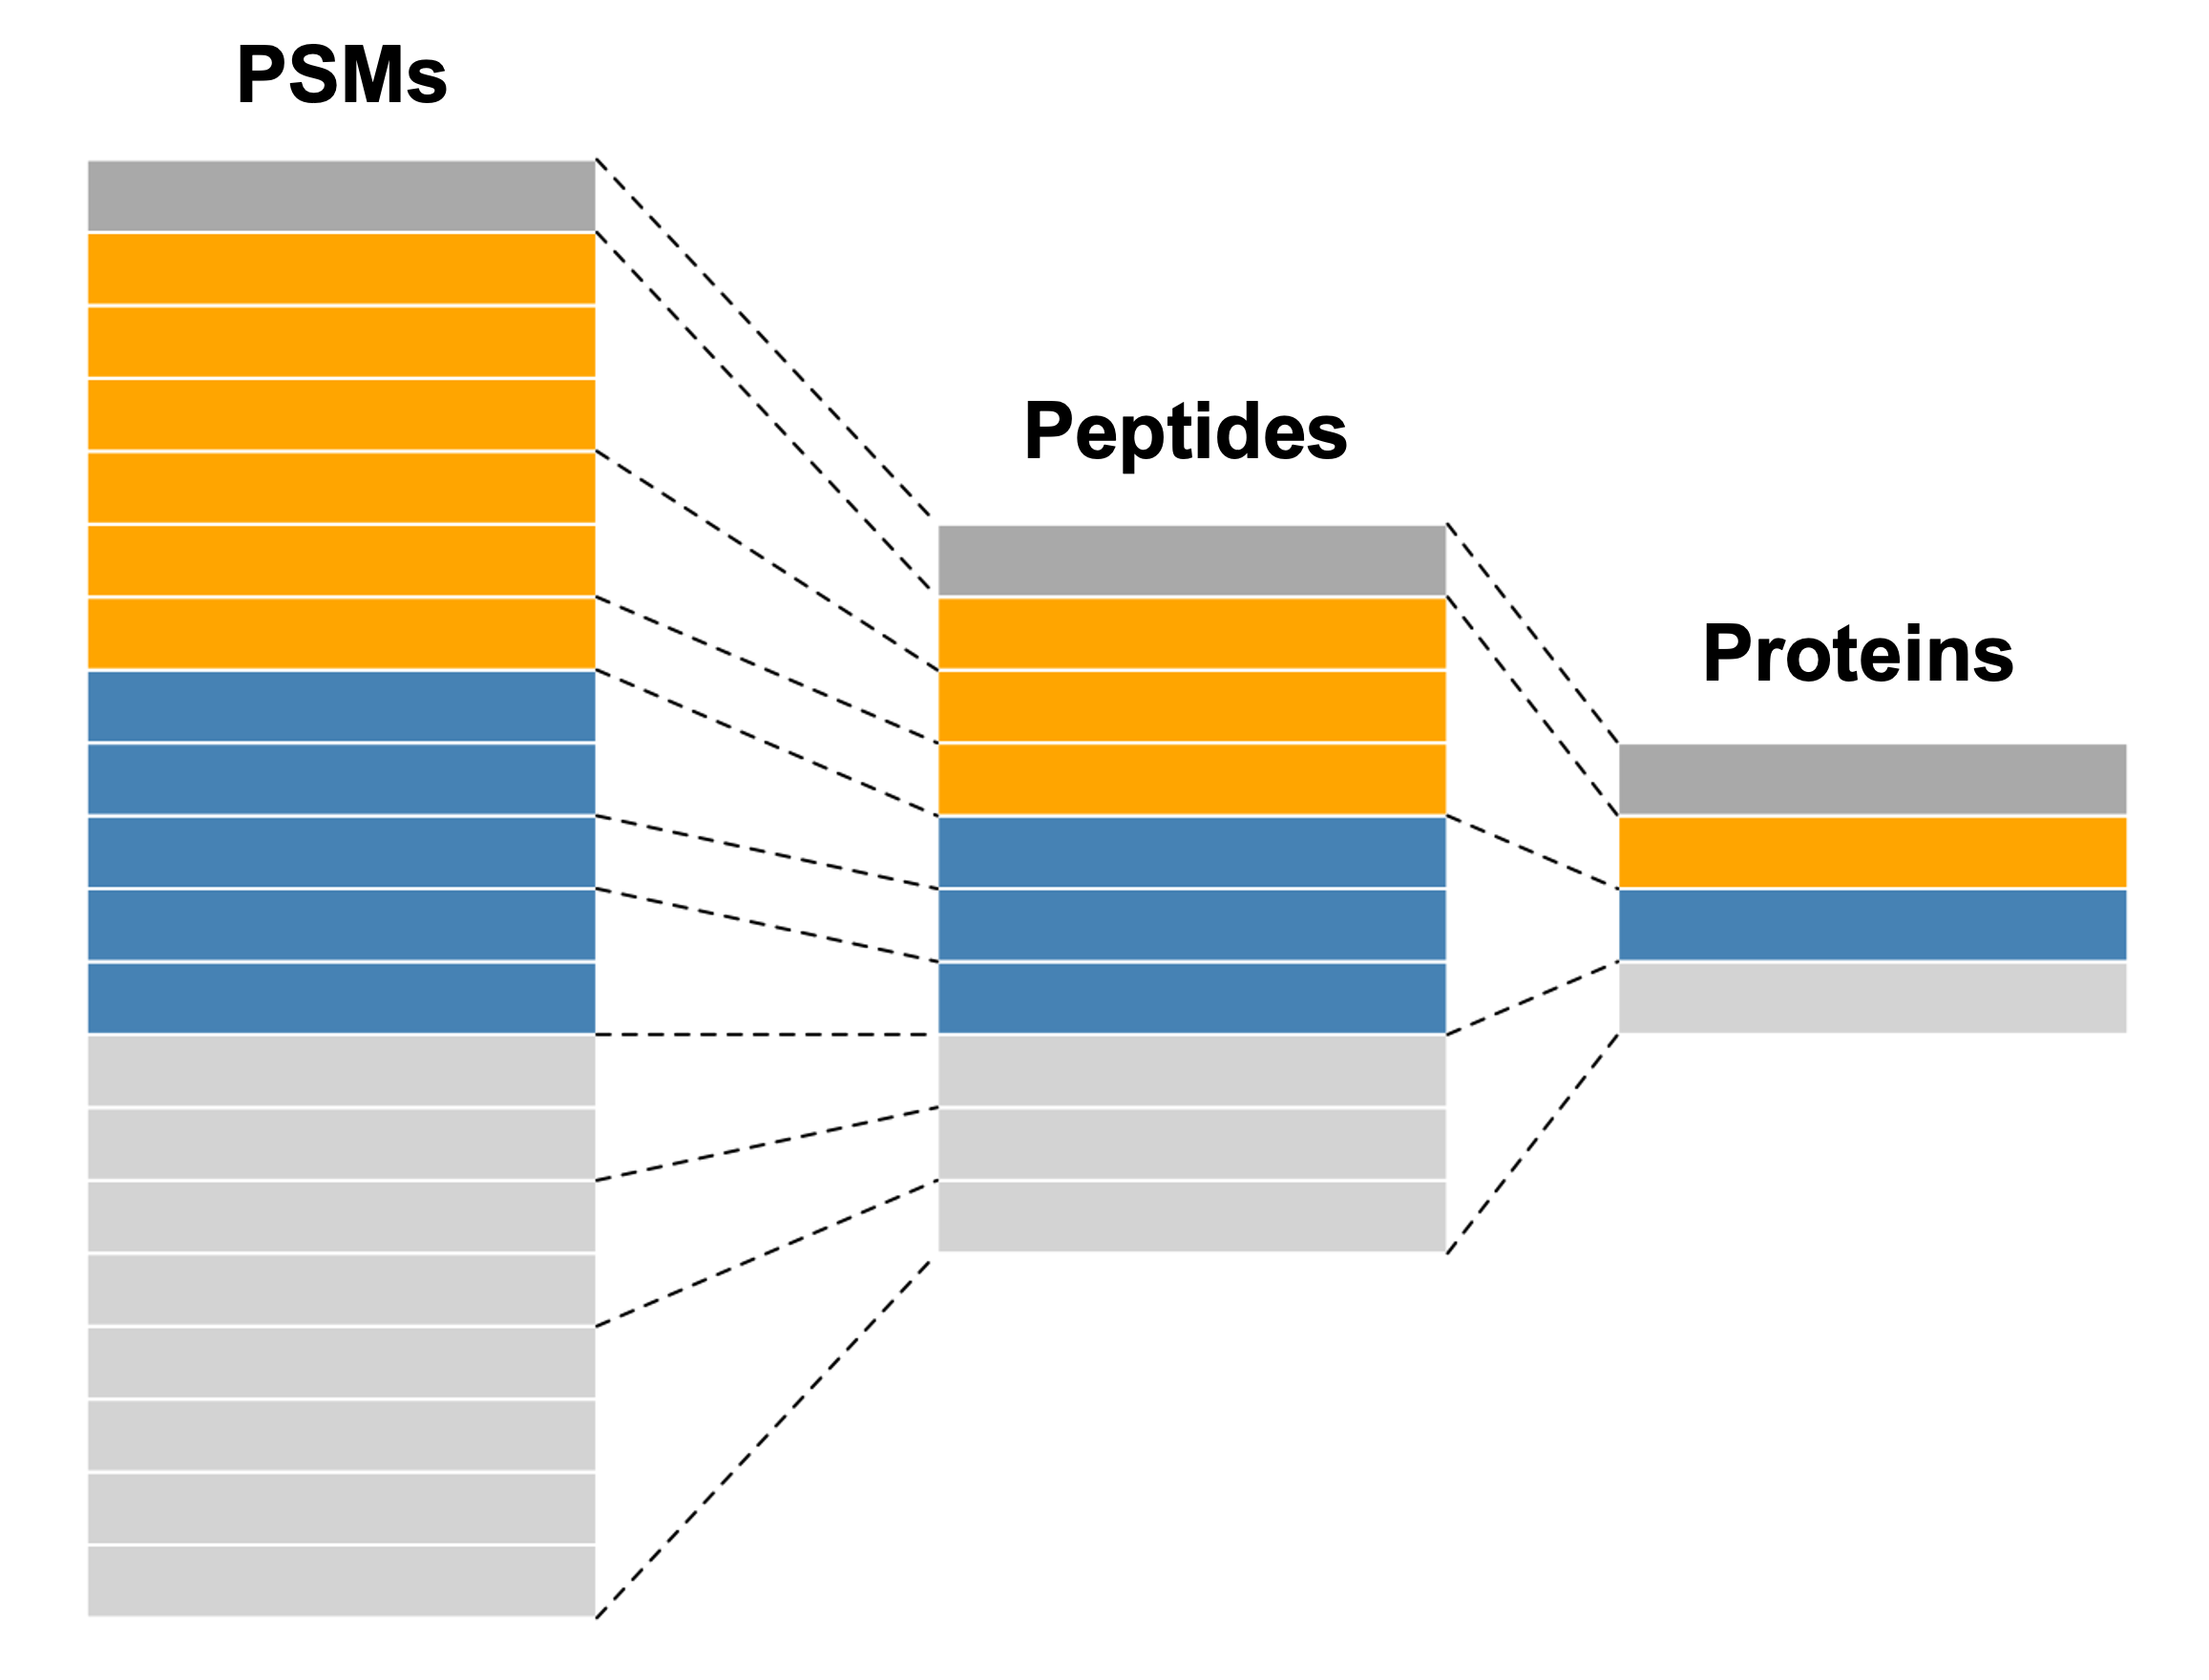
\includegraphics[width=1\linewidth]{Images/qfeatures} 

}

\caption{A graphic representation of the \texttt{QFeatures} object structure showing the relationship between assays. Figure modified from the \texttt{QFeatures} \citep{QFeat} vignette with permission.}\label{fig:qfeatures}
\end{figure}

\section{Processing and analysing quantitative TMT data}\label{processing-and-analysing-quantitative-tmt-data}

First, we provide a workflow for the processing and quality control of
quantitative TMT-labelled data. As outlined above, the cell pellet fractions of
triplicate control and treated HEK293 cells were labelled using a TMT6plex.
Labelling was as outlined in Table \ref{tab:table1}.

\begin{table}

\caption{\label{tab:table1}TMT labelling strategy in the use-case experiment}
\centering
\begin{tabular}[t]{l|l|r|l}
\hline
Sample Name & Condition & Replicate & Tag\\
\hline
S1 & Treated & 1 & TMT128\\
\hline
S2 & Treated & 2 & TMT127\\
\hline
S3 & Treated & 3 & TMT131\\
\hline
S4 & Control & 1 & TMT129\\
\hline
S5 & Control & 2 & TMT126\\
\hline
S6 & Control & 3 & TMT130\\
\hline
\end{tabular}
\end{table}

\subsection{Identification search of raw data}\label{identification-search-of-raw-data}

The first processing step in any MS-based proteomics experiment involves an
identification search using the raw data. The aim of this search is to identify
which peptide sequences, and therefore proteins, correspond to the raw spectra
output from the mass spectrometer. Several third-party software exist to
facilitate identification searches of raw MS data but ultimately the output of
any search is a list of PSMs, peptides and protein identifications along with
their corresponding quantification data.

The use-case data presented here was processed using Proteome Discoverer 2.5 and
additional information about this search is provided in the appendix. Further,
we provide template workflows for both the processing and consensus steps of the
Proteome Discoverer identification run in the supplementary information. It is
also possible to determine several of the key parameter settings during the
preliminary data exploration. This step will be particularly important for those
using publicly available data without detailed knowledge of the identification
search parameters. For now, we simply export the PSM-level \texttt{.txt} file from the
Proteome Discoverer output.

\subsection{Data import, housekeeping and exploration}\label{data-import-housekeeping-and-exploration}

\subsubsection{Importing data into R and creating a QFeatures object}\label{importing-data-into-r-and-creating-a-qfeatures-object}

Data cleaning, exploration and filtering at the PSM-level is performed in R
using \texttt{QFeatures}. First, data is imported from our PSM-level \texttt{.txt} file into a
\texttt{data.frame} using the base R \texttt{read.delim} function (the equivalent for \texttt{.csv}
files would be \texttt{read.csv}). This file should be stored within the users working
directory. Next, we use the \texttt{names} function to inspect the column names and
identify which columns contain quantitative data.

\begin{Shaded}
\begin{Highlighting}[]
\DocumentationTok{\#\# Locate the PSM .txt file}
\NormalTok{cp\_psm }\OtherTok{\textless{}{-}} \StringTok{"cell\_pellet\_tmt\_results\_psms.txt"}

\DocumentationTok{\#\# Import into a dataframe}
\NormalTok{cp\_df }\OtherTok{\textless{}{-}} \FunctionTok{read.delim}\NormalTok{(cp\_psm)}

\DocumentationTok{\#\# Identify columns containing quantitative data}
\NormalTok{cp\_df }\SpecialCharTok{\%\textgreater{}\%}
  \FunctionTok{names}\NormalTok{()}
\end{Highlighting}
\end{Shaded}

\begin{verbatim}
##  [1] "PSMs.Workflow.ID"                  "PSMs.Peptide.ID"                  
##  [3] "Checked"                           "Tags"                             
##  [5] "Confidence"                        "Identifying.Node.Type"            
##  [7] "Identifying.Node"                  "Search.ID"                        
##  [9] "Identifying.Node.No"               "PSM.Ambiguity"                    
## [11] "Sequence"                          "Annotated.Sequence"               
## [13] "Modifications"                     "Number.of.Proteins"               
## [15] "Master.Protein.Accessions"         "Master.Protein.Descriptions"      
## [17] "Protein.Accessions"                "Protein.Descriptions"             
## [19] "Number.of.Missed.Cleavages"        "Charge"                           
## [21] "Original.Precursor.Charge"         "Delta.Score"                      
## [23] "Delta.Cn"                          "Rank"                             
## [25] "Search.Engine.Rank"                "Concatenated.Rank"                
## [27] "mz.in.Da"                          "MHplus.in.Da"                     
## [29] "Theo.MHplus.in.Da"                 "Delta.M.in.ppm"                   
## [31] "Delta.mz.in.Da"                    "Ions.Matched"                     
## [33] "Matched.Ions"                      "Total.Ions"                       
## [35] "Intensity"                         "Activation.Type"                  
## [37] "NCE.in.Percent"                    "MS.Order"                         
## [39] "Isolation.Interference.in.Percent" "SPS.Mass.Matches.in.Percent"      
## [41] "Average.Reporter.SN"               "Ion.Inject.Time.in.ms"            
## [43] "RT.in.min"                         "First.Scan"                       
## [45] "Last.Scan"                         "Master.Scans"                     
## [47] "Spectrum.File"                     "File.ID"                          
## [49] "Abundance.126"                     "Abundance.127"                    
## [51] "Abundance.128"                     "Abundance.129"                    
## [53] "Abundance.130"                     "Abundance.131"                    
## [55] "Quan.Info"                         "Peptides.Matched"                 
## [57] "XCorr"                             "Number.of.Protein.Groups"         
## [59] "Percolator.q.Value"                "Percolator.PEP"                   
## [61] "Percolator.SVMScore"
\end{verbatim}

Now that the quantitative data columns have been identified, we can pass our
\texttt{data.frame} to the \texttt{readQFeatures} function and specify where our quantitative
columns are. The latter is done by passing either a numeric or character vector
to an argument called \texttt{quantCols} ( \texttt{ecols} in previous package versions).
Of note, the \texttt{readQFeatures} function can also take \texttt{fnames} as an argument to
specify a column to be used as the row names of the imported
object. Whilst previous \texttt{QFeatures} vignettes used the ``Sequence'' or
``Annotated.Sequence'' as row names, we advise against this because of the presence
of PSMs matched to the same peptide sequence with different modifications. In such
cases, multiple rows would have the same name forcing the \texttt{readQFeatures} function
to output a ``making assay row names unique'' message and add an identifying number
to the end of each duplicated row name. These sequences would then be considered
as unique during the aggregation of PSM to peptide, thus resulting in two independent
peptide- level quantitation values rather than one. Therefore, we do not pass a
\texttt{fnames} argument and the row names automatically become indices. Finally, we
pass the \texttt{name} argument to indicate the type of data added.

\begin{Shaded}
\begin{Highlighting}[]
\DocumentationTok{\#\# Create QFeatures }
\NormalTok{cp\_qf }\OtherTok{\textless{}{-}} \FunctionTok{readQFeatures}\NormalTok{(}\AttributeTok{assayData =}\NormalTok{ cp\_df,}
                       \AttributeTok{quantCols =} \DecValTok{49}\SpecialCharTok{:}\DecValTok{54}\NormalTok{,}
                       \AttributeTok{name =} \StringTok{"psms\_raw"}\NormalTok{)}
\end{Highlighting}
\end{Shaded}

\begin{verbatim}
## Checking arguments.
\end{verbatim}

\begin{verbatim}
## Loading data as a 'SummarizedExperiment' object.
\end{verbatim}

\begin{verbatim}
## Formatting sample annotations (colData).
\end{verbatim}

\begin{verbatim}
## Formatting data as a 'QFeatures' object.
\end{verbatim}

\subsubsection{\texorpdfstring{Accessing the \texttt{QFeatures} infrastructure}{Accessing the QFeatures infrastructure}}\label{accessing-the-qfeatures-infrastructure}

As outlined above, a \texttt{QFeatures} data object is a list of \texttt{SummarizedExperiment}
objects. As such, an individual \texttt{SummarizedExperiment} can be accessed using
the standard double bracket nomenclature, as demonstrated in the code chunk
below.

\begin{Shaded}
\begin{Highlighting}[]
\DocumentationTok{\#\# Index using position}
\NormalTok{cp\_qf[[}\DecValTok{1}\NormalTok{]]}
\end{Highlighting}
\end{Shaded}

\begin{verbatim}
## class: SummarizedExperiment 
## dim: 48832 6 
## metadata(0):
## assays(1): ''
## rownames(48832): 1 2 ... 48831 48832
## rowData names(55): PSMs.Workflow.ID PSMs.Peptide.ID ... Percolator.PEP
##   Percolator.SVMScore
## colnames(6): Abundance.126 Abundance.127 ... Abundance.130
##   Abundance.131
## colData names(0):
\end{verbatim}

\begin{Shaded}
\begin{Highlighting}[]
\DocumentationTok{\#\# Index using name}
\NormalTok{cp\_qf[[}\StringTok{"psms\_raw"}\NormalTok{]]}
\end{Highlighting}
\end{Shaded}

\begin{verbatim}
## class: SummarizedExperiment 
## dim: 48832 6 
## metadata(0):
## assays(1): ''
## rownames(48832): 1 2 ... 48831 48832
## rowData names(55): PSMs.Workflow.ID PSMs.Peptide.ID ... Percolator.PEP
##   Percolator.SVMScore
## colnames(6): Abundance.126 Abundance.127 ... Abundance.130
##   Abundance.131
## colData names(0):
\end{verbatim}

A summary of the data contained in the slots is printed to the screen.
To retrieve the \texttt{rowData}, \texttt{colData} or \texttt{assay} data from a particular
\texttt{SummarizedExperiment} within a \texttt{QFeatures} object users can make use of the
\texttt{rowData}, \texttt{colData} and \texttt{assay} functions. For plotting or data transformation
it is necessary to convert to a \texttt{data.frame} or \texttt{tibble}.

\begin{Shaded}
\begin{Highlighting}[]
\DocumentationTok{\#\# Access feature information with rowData}
\DocumentationTok{\#\# The output should be converted to data.frame/tibble for further processing}
\NormalTok{cp\_qf[[}\StringTok{"psms\_raw"}\NormalTok{]] }\SpecialCharTok{\%\textgreater{}\%} 
  \FunctionTok{rowData}\NormalTok{() }\SpecialCharTok{\%\textgreater{}\%} 
  \FunctionTok{as\_tibble}\NormalTok{() }\SpecialCharTok{\%\textgreater{}\%} 
  \FunctionTok{summarise}\NormalTok{(}\AttributeTok{mean\_intensity =} \FunctionTok{mean}\NormalTok{(Intensity))}
\end{Highlighting}
\end{Shaded}

\begin{verbatim}
## # A tibble: 1 x 1
##   mean_intensity
##            <dbl>
## 1      13281497.
\end{verbatim}

To ensure that quantitative data has been correctly imported in as a numeric
variable, we can look at the \texttt{assay} slot.

\begin{Shaded}
\begin{Highlighting}[]
\DocumentationTok{\#\# Look at top 6 rows of the assay (quantitative data)}
\NormalTok{cp\_qf[[}\StringTok{"psms\_raw"}\NormalTok{]] }\SpecialCharTok{\%\textgreater{}\%}
  \FunctionTok{assay}\NormalTok{() }\SpecialCharTok{\%\textgreater{}\%}
  \FunctionTok{head}\NormalTok{() }
\end{Highlighting}
\end{Shaded}

\begin{verbatim}
##   Abundance.126 Abundance.127 Abundance.128 Abundance.129 Abundance.130
## 1            NA            NA            NA            NA            NA
## 2            NA            NA            NA            NA            NA
## 3            NA            NA            NA            NA            NA
## 4          14.1          18.1          11.8           9.4          18.9
## 5            NA           2.5            NA           3.4           3.2
## 6          16.7          26.2          18.7          22.4          25.3
##   Abundance.131
## 1            NA
## 2            NA
## 3            NA
## 4          13.5
## 5            NA
## 6          17.2
\end{verbatim}

\begin{Shaded}
\begin{Highlighting}[]
\DocumentationTok{\#\# Confirm numeric assay}
\NormalTok{cp\_qf[[}\StringTok{"psms\_raw"}\NormalTok{]] }\SpecialCharTok{\%\textgreater{}\%}
  \FunctionTok{assay}\NormalTok{() }\SpecialCharTok{\%\textgreater{}\%}
  \FunctionTok{type}\NormalTok{()}
\end{Highlighting}
\end{Shaded}

\begin{verbatim}
## [1] "double"
\end{verbatim}

Our \texttt{assay} contains data of type \texttt{double}, a sub-type of numeric data in R. If
users find that their quantitative data is of type \texttt{character}, it is necessary
to correct this before moving on with the rest of the workflow.

\subsubsection{Adding metadata}\label{adding-metadata}

Having imported the data, each sample is first annotated with its TMT label,
sample reference and condition. As this information is experimental metadata, it
is added to the \texttt{colData} slot. It is important for users check that the \texttt{colData}
annotations correspond to their correct samples, particularly if the column order
in the imported results file does not align with the sample order. This is the
case for the use-case data since TMT labels were randomized in an attempt to
minimze the effect of TMT channel leakage.

\begin{Shaded}
\begin{Highlighting}[]
\DocumentationTok{\#\# Add sample info as colData to QFeatures object}
\NormalTok{cp\_qf}\SpecialCharTok{$}\NormalTok{label }\OtherTok{\textless{}{-}} \FunctionTok{c}\NormalTok{(}\StringTok{"TMT126"}\NormalTok{,}
                 \StringTok{"TMT127"}\NormalTok{,}
                 \StringTok{"TMT128"}\NormalTok{,}
                 \StringTok{"TMT129"}\NormalTok{,}
                 \StringTok{"TMT130"}\NormalTok{,}
                 \StringTok{"TMT131"}\NormalTok{)}

\NormalTok{cp\_qf}\SpecialCharTok{$}\NormalTok{sample }\OtherTok{\textless{}{-}} \FunctionTok{c}\NormalTok{(}\StringTok{"S5"}\NormalTok{, }\StringTok{"S2"}\NormalTok{, }\StringTok{"S1"}\NormalTok{, }\StringTok{"S4"}\NormalTok{, }\StringTok{"S6"}\NormalTok{, }\StringTok{"S3"}\NormalTok{)}

\NormalTok{cp\_qf}\SpecialCharTok{$}\NormalTok{condition }\OtherTok{\textless{}{-}} \FunctionTok{c}\NormalTok{(}\StringTok{"Control"}\NormalTok{, }\StringTok{"Treated"}\NormalTok{, }\StringTok{"Treated"}\NormalTok{,}
                     \StringTok{"Control"}\NormalTok{, }\StringTok{"Control"}\NormalTok{, }\StringTok{"Treated"}\NormalTok{)}

\DocumentationTok{\#\# Verify}
\FunctionTok{colData}\NormalTok{(cp\_qf)}
\end{Highlighting}
\end{Shaded}

\begin{verbatim}
## DataFrame with 6 rows and 3 columns
##                     label      sample   condition
##               <character> <character> <character>
## Abundance.126      TMT126          S5     Control
## Abundance.127      TMT127          S2     Treated
## Abundance.128      TMT128          S1     Treated
## Abundance.129      TMT129          S4     Control
## Abundance.130      TMT130          S6     Control
## Abundance.131      TMT131          S3     Treated
\end{verbatim}

\begin{Shaded}
\begin{Highlighting}[]
\DocumentationTok{\#\# Assign the colData to first assay as well}
\FunctionTok{colData}\NormalTok{(cp\_qf[[}\StringTok{"psms\_raw"}\NormalTok{]]) }\OtherTok{\textless{}{-}} \FunctionTok{colData}\NormalTok{(cp\_qf)}
\end{Highlighting}
\end{Shaded}

It is also useful to clean up sample names such that they are short, intuitive
and informative. This is done by editing the \texttt{colnames}. These steps may not
always be necessary depending upon the identification search output.

\begin{Shaded}
\begin{Highlighting}[]
\DocumentationTok{\#\# Clean sample names}
\FunctionTok{colnames}\NormalTok{(cp\_qf[[}\StringTok{"psms\_raw"}\NormalTok{]]) }\OtherTok{\textless{}{-}} \FunctionTok{c}\NormalTok{(}\StringTok{"S5"}\NormalTok{, }\StringTok{"S2"}\NormalTok{, }\StringTok{"S1"}\NormalTok{, }\StringTok{"S4"}\NormalTok{, }\StringTok{"S6"}\NormalTok{, }\StringTok{"S3"}\NormalTok{)}
\end{Highlighting}
\end{Shaded}

\subsubsection{Preliminary data exploration}\label{preliminary-data-exploration}

As well as cleaning and annotating the data, it is always advisable to check
that the import worked and that the data looks as expected. Further, preliminary
exploration of the data can provide an early sign of whether the experiment and
subsequent identification search were successful. Importantly, however, the
names of key parameters will vary depending on the software used, and will
likely change over time. Users will need to be aware of this and modify the code
in this workflow accordingly.

\begin{Shaded}
\begin{Highlighting}[]
\DocumentationTok{\#\# Check what information has been imported}
\NormalTok{cp\_qf[[}\StringTok{"psms\_raw"}\NormalTok{]] }\SpecialCharTok{\%\textgreater{}\%}
  \FunctionTok{rowData}\NormalTok{() }\SpecialCharTok{\%\textgreater{}\%}
  \FunctionTok{colnames}\NormalTok{()}
\end{Highlighting}
\end{Shaded}

\begin{verbatim}
##  [1] "PSMs.Workflow.ID"                  "PSMs.Peptide.ID"                  
##  [3] "Checked"                           "Tags"                             
##  [5] "Confidence"                        "Identifying.Node.Type"            
##  [7] "Identifying.Node"                  "Search.ID"                        
##  [9] "Identifying.Node.No"               "PSM.Ambiguity"                    
## [11] "Sequence"                          "Annotated.Sequence"               
## [13] "Modifications"                     "Number.of.Proteins"               
## [15] "Master.Protein.Accessions"         "Master.Protein.Descriptions"      
## [17] "Protein.Accessions"                "Protein.Descriptions"             
## [19] "Number.of.Missed.Cleavages"        "Charge"                           
## [21] "Original.Precursor.Charge"         "Delta.Score"                      
## [23] "Delta.Cn"                          "Rank"                             
## [25] "Search.Engine.Rank"                "Concatenated.Rank"                
## [27] "mz.in.Da"                          "MHplus.in.Da"                     
## [29] "Theo.MHplus.in.Da"                 "Delta.M.in.ppm"                   
## [31] "Delta.mz.in.Da"                    "Ions.Matched"                     
## [33] "Matched.Ions"                      "Total.Ions"                       
## [35] "Intensity"                         "Activation.Type"                  
## [37] "NCE.in.Percent"                    "MS.Order"                         
## [39] "Isolation.Interference.in.Percent" "SPS.Mass.Matches.in.Percent"      
## [41] "Average.Reporter.SN"               "Ion.Inject.Time.in.ms"            
## [43] "RT.in.min"                         "First.Scan"                       
## [45] "Last.Scan"                         "Master.Scans"                     
## [47] "Spectrum.File"                     "File.ID"                          
## [49] "Quan.Info"                         "Peptides.Matched"                 
## [51] "XCorr"                             "Number.of.Protein.Groups"         
## [53] "Percolator.q.Value"                "Percolator.PEP"                   
## [55] "Percolator.SVMScore"
\end{verbatim}

\begin{Shaded}
\begin{Highlighting}[]
\DocumentationTok{\#\# Find out how many PSMs are in the data}
\NormalTok{cp\_qf[[}\StringTok{"psms\_raw"}\NormalTok{]] }\SpecialCharTok{\%\textgreater{}\%}
  \FunctionTok{dim}\NormalTok{()}
\end{Highlighting}
\end{Shaded}

\begin{verbatim}
## [1] 48832     6
\end{verbatim}

\begin{Shaded}
\begin{Highlighting}[]
\NormalTok{original\_psms }\OtherTok{\textless{}{-}}\NormalTok{ cp\_qf[[}\StringTok{"psms\_raw"}\NormalTok{]] }\SpecialCharTok{\%\textgreater{}\%}
  \FunctionTok{nrow}\NormalTok{() }\SpecialCharTok{\%\textgreater{}\%}
  \FunctionTok{as.numeric}\NormalTok{()}
\end{Highlighting}
\end{Shaded}

We can see that the original data includes 48832 PSMs
across the 6 samples. It is also useful to make note of how many peptides and
proteins the raw PSM data corresponds to, and to track how many we remove during
the subsequent filtering steps. This can be done by checking how many unique entries
are located within the ``Sequence'' and ``Master.Protein.Accessions'' for peptides
and proteins, respectively. Of note, searching for unique peptide sequences means
that the number of peptides does not include duplicated sequences with different
modifications.

\begin{Shaded}
\begin{Highlighting}[]
\DocumentationTok{\#\# Find out how many peptides and master proteins are in the data}
\NormalTok{original\_peps }\OtherTok{\textless{}{-}}\NormalTok{ cp\_qf[[}\StringTok{"psms\_raw"}\NormalTok{]] }\SpecialCharTok{\%\textgreater{}\%} 
  \FunctionTok{rowData}\NormalTok{() }\SpecialCharTok{\%\textgreater{}\%} 
  \FunctionTok{as\_tibble}\NormalTok{() }\SpecialCharTok{\%\textgreater{}\%} 
  \FunctionTok{pull}\NormalTok{(Sequence) }\SpecialCharTok{\%\textgreater{}\%} 
  \FunctionTok{unique}\NormalTok{() }\SpecialCharTok{\%\textgreater{}\%}
  \FunctionTok{length}\NormalTok{() }\SpecialCharTok{\%\textgreater{}\%}
  \FunctionTok{as.numeric}\NormalTok{()}

\NormalTok{original\_prots }\OtherTok{\textless{}{-}}\NormalTok{ cp\_qf[[}\StringTok{"psms\_raw"}\NormalTok{]] }\SpecialCharTok{\%\textgreater{}\%} 
  \FunctionTok{rowData}\NormalTok{() }\SpecialCharTok{\%\textgreater{}\%} 
  \FunctionTok{as\_tibble}\NormalTok{() }\SpecialCharTok{\%\textgreater{}\%} 
  \FunctionTok{pull}\NormalTok{(Master.Protein.Accessions) }\SpecialCharTok{\%\textgreater{}\%} 
  \FunctionTok{unique}\NormalTok{() }\SpecialCharTok{\%\textgreater{}\%}
  \FunctionTok{length}\NormalTok{() }\SpecialCharTok{\%\textgreater{}\%}
  \FunctionTok{as.numeric}\NormalTok{()}

\FunctionTok{print}\NormalTok{(}\FunctionTok{c}\NormalTok{(original\_peps, original\_prots))}
\end{Highlighting}
\end{Shaded}

\begin{verbatim}
## [1] 25969  5040
\end{verbatim}

Hence, the output of the identification search contains
48832 PSMs corresponding to
25969 peptide sequences and
5040 master proteins. Finally, we
confirm that the identification search was carried out as expected. For this, we
print summaries of the key search parameters using the \texttt{table} function for
discrete parameters and \texttt{summary} for those which are continuous. This is also
helpful for users who are analyzing publicly available data and have limited
knowledge about the identification search parameters.

\begin{Shaded}
\begin{Highlighting}[]
\DocumentationTok{\#\# Check missed cleavages}
\NormalTok{cp\_qf[[}\StringTok{"psms\_raw"}\NormalTok{]] }\SpecialCharTok{\%\textgreater{}\%}
  \FunctionTok{rowData}\NormalTok{() }\SpecialCharTok{\%\textgreater{}\%} 
  \FunctionTok{as\_tibble}\NormalTok{() }\SpecialCharTok{\%\textgreater{}\%} 
  \FunctionTok{pull}\NormalTok{(Number.of.Missed.Cleavages) }\SpecialCharTok{\%\textgreater{}\%} 
  \FunctionTok{table}\NormalTok{()}
\end{Highlighting}
\end{Shaded}

\begin{verbatim}
## .
##     0     1     2 
## 46164  2592    76
\end{verbatim}

\begin{Shaded}
\begin{Highlighting}[]
\DocumentationTok{\#\# Check precursor mass tolerance}
\NormalTok{cp\_qf[[}\StringTok{"psms\_raw"}\NormalTok{]] }\SpecialCharTok{\%\textgreater{}\%} 
  \FunctionTok{rowData}\NormalTok{() }\SpecialCharTok{\%\textgreater{}\%} 
  \FunctionTok{as\_tibble}\NormalTok{() }\SpecialCharTok{\%\textgreater{}\%} 
  \FunctionTok{pull}\NormalTok{(Delta.M.in.ppm) }\SpecialCharTok{\%\textgreater{}\%} 
  \FunctionTok{summary}\NormalTok{()}
\end{Highlighting}
\end{Shaded}

\begin{verbatim}
##    Min. 1st Qu.  Median    Mean 3rd Qu.    Max. 
## -8.9300 -0.6000  0.3700  0.6447  1.3100  9.6700
\end{verbatim}

\begin{Shaded}
\begin{Highlighting}[]
\DocumentationTok{\#\# Check fragment mass tolerance}
\NormalTok{cp\_qf[[}\StringTok{"psms\_raw"}\NormalTok{]] }\SpecialCharTok{\%\textgreater{}\%} 
  \FunctionTok{rowData}\NormalTok{() }\SpecialCharTok{\%\textgreater{}\%} 
  \FunctionTok{as\_tibble}\NormalTok{() }\SpecialCharTok{\%\textgreater{}\%} 
  \FunctionTok{pull}\NormalTok{(Delta.mz.in.Da) }\SpecialCharTok{\%\textgreater{}\%} 
  \FunctionTok{summary}\NormalTok{()}
\end{Highlighting}
\end{Shaded}

\begin{verbatim}
##       Min.    1st Qu.     Median       Mean    3rd Qu.       Max. 
## -0.0110400 -0.0004100  0.0002500  0.0006812  0.0010200  0.0135100
\end{verbatim}

\begin{Shaded}
\begin{Highlighting}[]
\DocumentationTok{\#\# Check PSM confidence allocations}
\NormalTok{cp\_qf[[}\StringTok{"psms\_raw"}\NormalTok{]] }\SpecialCharTok{\%\textgreater{}\%} 
  \FunctionTok{rowData}\NormalTok{() }\SpecialCharTok{\%\textgreater{}\%} 
  \FunctionTok{as\_tibble}\NormalTok{() }\SpecialCharTok{\%\textgreater{}\%} 
  \FunctionTok{pull}\NormalTok{(Confidence) }\SpecialCharTok{\%\textgreater{}\%} 
  \FunctionTok{table}\NormalTok{()}
\end{Highlighting}
\end{Shaded}

\begin{verbatim}
## .
##  High 
## 48832
\end{verbatim}

\subsection{Experimental quality control checks}\label{experimental-quality-control-checks}

Experimental quality control of TMT-labelled quantitive proteomics data takes
place in two steps: (1) assessment of the raw mass spectrometry data, and (2)
evaluation of TMT labelling efficiency.

\subsubsection{Quality control of the raw mass spectrometry data}\label{quality-control-of-the-raw-mass-spectrometry-data}

Having taken an initial look at the output of the identification search, it is
possible to create some simple plots to inspect the raw mass spectrometry data.
Such plots are useful in revealing problems that may have occurred during
the mass spectrometry run but are far from extensive. Users who wish to carry
out a more in-depth evaluation of the raw mass spectrometry data may benefit
from use of the
\href{https://bioconductor.org/packages/release/bioc/html/Spectra.html}{\texttt{Spectra} Bioconductor package}
which allows for visualization and exploration of raw chromatograms and spectra,
among other features \citep{Rainer2022}.

The first plot we generate looks at the delta precursor mass, that is the
difference between observed and estimated precursor mass, across retention time.
Importantly, exploration of this raw data feature can only be done when using
the raw data prior to recalibration. For users of Proteome Discoverer, this
means using the spectral files node rather than the spectral files recalibration
node.

\begin{Shaded}
\begin{Highlighting}[]
\DocumentationTok{\#\# Generate scatter plot of mass accuracy}
\NormalTok{cp\_qf[[}\StringTok{"psms\_raw"}\NormalTok{]] }\SpecialCharTok{\%\textgreater{}\%}
  \FunctionTok{rowData}\NormalTok{() }\SpecialCharTok{\%\textgreater{}\%} 
  \FunctionTok{as\_tibble}\NormalTok{() }\SpecialCharTok{\%\textgreater{}\%}
  \FunctionTok{ggplot}\NormalTok{(}\FunctionTok{aes}\NormalTok{(}\AttributeTok{x =}\NormalTok{ RT.in.min, }\AttributeTok{y =}\NormalTok{ Delta.M.in.ppm)) }\SpecialCharTok{+}
  \FunctionTok{geom\_point}\NormalTok{(}\AttributeTok{size =} \FloatTok{0.5}\NormalTok{, }\AttributeTok{shape =} \DecValTok{4}\NormalTok{) }\SpecialCharTok{+}
  \FunctionTok{geom\_hline}\NormalTok{(}\AttributeTok{yintercept =} \DecValTok{5}\NormalTok{, }\AttributeTok{linetype =} \StringTok{"dashed"}\NormalTok{, }\AttributeTok{color =} \StringTok{"red"}\NormalTok{) }\SpecialCharTok{+}
  \FunctionTok{geom\_hline}\NormalTok{(}\AttributeTok{yintercept =} \SpecialCharTok{{-}}\DecValTok{5}\NormalTok{, }\AttributeTok{linetype =} \StringTok{"dashed"}\NormalTok{, }\AttributeTok{color =} \StringTok{"red"}\NormalTok{) }\SpecialCharTok{+}
  \FunctionTok{labs}\NormalTok{(}\AttributeTok{x =} \StringTok{"RT (min)"}\NormalTok{, }\AttributeTok{y =} \StringTok{"Delta precursor mass (ppm)"}\NormalTok{) }\SpecialCharTok{+}
  \FunctionTok{scale\_x\_continuous}\NormalTok{(}\AttributeTok{limits =} \FunctionTok{c}\NormalTok{(}\DecValTok{0}\NormalTok{, }\DecValTok{120}\NormalTok{), }\AttributeTok{breaks =} \FunctionTok{seq}\NormalTok{(}\DecValTok{0}\NormalTok{, }\DecValTok{120}\NormalTok{, }\DecValTok{20}\NormalTok{)) }\SpecialCharTok{+}
  \FunctionTok{scale\_y\_continuous}\NormalTok{(}\AttributeTok{limits =} \FunctionTok{c}\NormalTok{(}\SpecialCharTok{{-}}\DecValTok{10}\NormalTok{, }\DecValTok{10}\NormalTok{), }\AttributeTok{breaks =} \FunctionTok{c}\NormalTok{(}\SpecialCharTok{{-}}\DecValTok{10}\NormalTok{, }\SpecialCharTok{{-}}\DecValTok{5}\NormalTok{, }\DecValTok{0}\NormalTok{, }\DecValTok{5}\NormalTok{, }\DecValTok{10}\NormalTok{)) }\SpecialCharTok{+}
  \FunctionTok{ggtitle}\NormalTok{(}\StringTok{"PSM retention time against delta precursor mass"}\NormalTok{) }\SpecialCharTok{+}
  \FunctionTok{theme\_bw}\NormalTok{()}
\end{Highlighting}
\end{Shaded}

\begin{center}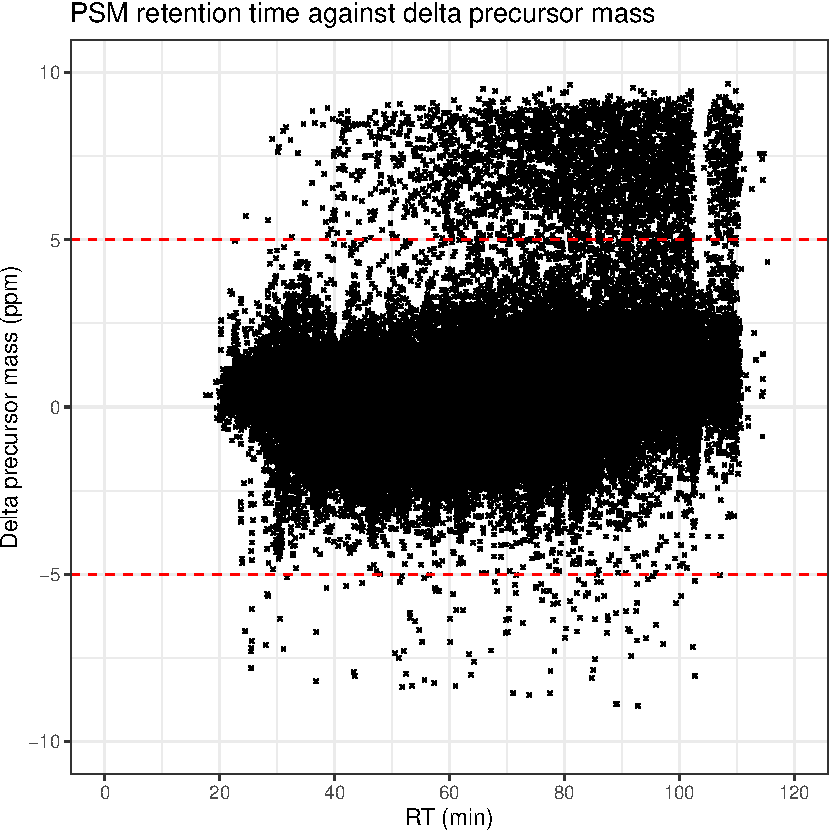
\includegraphics[height=0.3\textheight]{workflow_expressions_files/figure-latex/tmt_mass_accuracy-1} \end{center}

Since we applied a precursor mass tolerance of 10 ppm during the identification
search, all of the PSMs are within ±10 ppm. Ideally, however, we want the
majority of the data to be within ±5 ppm since smaller delta masses correspond
to a greater rate of correct peptide identifications. From the graph we have
plotted we can see that indeed the majority of PSMs are within ±5 ppm. If users
find that too many PSMs are outside of the desired ±5 ppm, it is advisable to
check the calibration of the mass spectrometer.

The second quality control plot of raw data is that of MS2 ion inject time
across the retention time gradient. Here, it is desirable to achieve an average
MS2 injection time of 50 ms or less, although the exact target threshold will
depend upon the sample load. If the average ion inject time is longer than
desired, then the ion transfer tube and/or front end optics of the instrument may
require cleaning.

\begin{Shaded}
\begin{Highlighting}[]
\DocumentationTok{\#\# Generate scatter plot of ion inject time across retention time}
\NormalTok{cp\_qf[[}\StringTok{"psms\_raw"}\NormalTok{]] }\SpecialCharTok{\%\textgreater{}\%}
  \FunctionTok{rowData}\NormalTok{() }\SpecialCharTok{\%\textgreater{}\%} 
  \FunctionTok{as\_tibble}\NormalTok{() }\SpecialCharTok{\%\textgreater{}\%}
  \FunctionTok{ggplot}\NormalTok{(}\FunctionTok{aes}\NormalTok{(}\AttributeTok{x =}\NormalTok{ RT.in.min, }\AttributeTok{y =}\NormalTok{ Ion.Inject.Time.in.ms)) }\SpecialCharTok{+}
  \FunctionTok{geom\_point}\NormalTok{(}\AttributeTok{size =} \FloatTok{0.5}\NormalTok{, }\AttributeTok{shape =} \DecValTok{4}\NormalTok{) }\SpecialCharTok{+}
  \FunctionTok{geom\_hline}\NormalTok{(}\AttributeTok{yintercept =} \DecValTok{50}\NormalTok{, }\AttributeTok{linetype =} \StringTok{"dashed"}\NormalTok{, }\AttributeTok{color =} \StringTok{"red"}\NormalTok{) }\SpecialCharTok{+}
  \FunctionTok{labs}\NormalTok{(}\AttributeTok{x =} \StringTok{"RT (min)"}\NormalTok{, }\AttributeTok{y =} \StringTok{"Ion inject time (ms)"}\NormalTok{) }\SpecialCharTok{+}
  \FunctionTok{scale\_x\_continuous}\NormalTok{(}\AttributeTok{limits =} \FunctionTok{c}\NormalTok{(}\DecValTok{0}\NormalTok{, }\DecValTok{120}\NormalTok{), }\AttributeTok{breaks =} \FunctionTok{seq}\NormalTok{(}\DecValTok{0}\NormalTok{, }\DecValTok{120}\NormalTok{, }\DecValTok{20}\NormalTok{)) }\SpecialCharTok{+}
  \FunctionTok{scale\_y\_continuous}\NormalTok{(}\AttributeTok{limits =} \FunctionTok{c}\NormalTok{(}\DecValTok{0}\NormalTok{, }\DecValTok{60}\NormalTok{), }\AttributeTok{breaks =} \FunctionTok{seq}\NormalTok{(}\DecValTok{0}\NormalTok{, }\DecValTok{60}\NormalTok{, }\DecValTok{10}\NormalTok{)) }\SpecialCharTok{+}
  \FunctionTok{ggtitle}\NormalTok{(}\StringTok{"PSM retention time against ion inject time"}\NormalTok{) }\SpecialCharTok{+}
  \FunctionTok{theme\_bw}\NormalTok{()}
\end{Highlighting}
\end{Shaded}

\begin{center}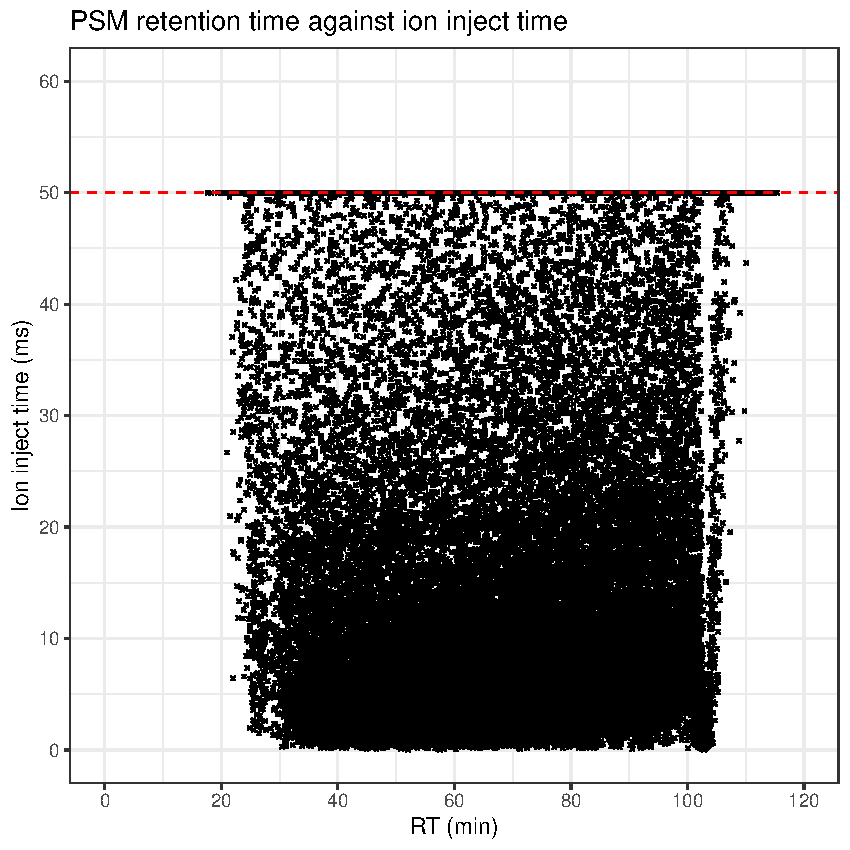
\includegraphics[height=0.3\textheight]{workflow_expressions_files/figure-latex/tmt_ion_injection_1-1} \end{center}

From this plot we can see that whilst there is a high density of PSMs at low
inject times, there are also many data points found at the 50 ms threshold. This
indicates that by increasing the time allowed for ions to accumulate in the ion
trap, the number of PSMs could also have been increased. Finally, we inspect the
distribution of PSMs across both the ion injection time and retention time by
plotting histograms.

\begin{Shaded}
\begin{Highlighting}[]
\DocumentationTok{\#\# Plot histogram of PSM ion inject time}
\NormalTok{cp\_qf[[}\StringTok{"psms\_raw"}\NormalTok{]] }\SpecialCharTok{\%\textgreater{}\%}
  \FunctionTok{rowData}\NormalTok{() }\SpecialCharTok{\%\textgreater{}\%} 
  \FunctionTok{as\_tibble}\NormalTok{() }\SpecialCharTok{\%\textgreater{}\%}
  \FunctionTok{ggplot}\NormalTok{(}\FunctionTok{aes}\NormalTok{(}\AttributeTok{x =}\NormalTok{ Ion.Inject.Time.in.ms)) }\SpecialCharTok{+}
  \FunctionTok{geom\_histogram}\NormalTok{(}\AttributeTok{binwidth =} \DecValTok{1}\NormalTok{) }\SpecialCharTok{+}
  \FunctionTok{labs}\NormalTok{(}\AttributeTok{x =} \StringTok{"Ion inject time (ms)"}\NormalTok{, }\AttributeTok{y =} \StringTok{"Frequency"}\NormalTok{) }\SpecialCharTok{+}
  \FunctionTok{scale\_x\_continuous}\NormalTok{(}\AttributeTok{limits =} \FunctionTok{c}\NormalTok{(}\SpecialCharTok{{-}}\FloatTok{0.5}\NormalTok{, }\FloatTok{52.5}\NormalTok{), }\AttributeTok{breaks =} \FunctionTok{seq}\NormalTok{(}\DecValTok{0}\NormalTok{, }\DecValTok{50}\NormalTok{, }\DecValTok{5}\NormalTok{)) }\SpecialCharTok{+}
  \FunctionTok{ggtitle}\NormalTok{(}\StringTok{"PSM frequency across ion injection time"}\NormalTok{) }\SpecialCharTok{+}
  \FunctionTok{theme\_bw}\NormalTok{()}
\end{Highlighting}
\end{Shaded}

\begin{center}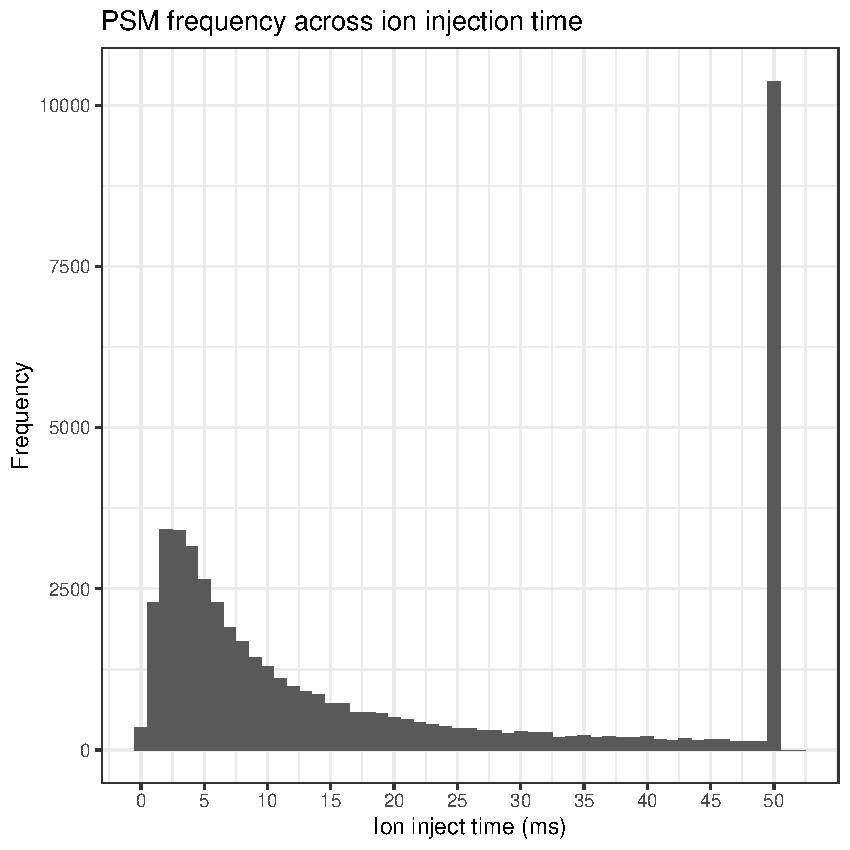
\includegraphics[height=0.3\textheight]{workflow_expressions_files/figure-latex/tmt_ion_injection_2-1} \end{center}

\begin{Shaded}
\begin{Highlighting}[]
\DocumentationTok{\#\# Plot histogram of PSM retention time}
\NormalTok{cp\_qf[[}\StringTok{"psms\_raw"}\NormalTok{]] }\SpecialCharTok{\%\textgreater{}\%}
  \FunctionTok{rowData}\NormalTok{() }\SpecialCharTok{\%\textgreater{}\%} 
  \FunctionTok{as\_tibble}\NormalTok{() }\SpecialCharTok{\%\textgreater{}\%}
  \FunctionTok{ggplot}\NormalTok{(}\FunctionTok{aes}\NormalTok{(}\AttributeTok{x =}\NormalTok{ RT.in.min)) }\SpecialCharTok{+}
  \FunctionTok{geom\_histogram}\NormalTok{(}\AttributeTok{binwidth =} \DecValTok{1}\NormalTok{) }\SpecialCharTok{+}
  \FunctionTok{labs}\NormalTok{(}\AttributeTok{x =} \StringTok{"RT (min)"}\NormalTok{, }\AttributeTok{y =} \StringTok{"Frequency"}\NormalTok{) }\SpecialCharTok{+}
  \FunctionTok{scale\_x\_continuous}\NormalTok{(}\AttributeTok{breaks =} \FunctionTok{seq}\NormalTok{(}\DecValTok{0}\NormalTok{, }\DecValTok{120}\NormalTok{, }\DecValTok{20}\NormalTok{)) }\SpecialCharTok{+}
  \FunctionTok{ggtitle}\NormalTok{(}\StringTok{"PSM frequency across retention time"}\NormalTok{) }\SpecialCharTok{+}
  \FunctionTok{theme\_bw}\NormalTok{()}
\end{Highlighting}
\end{Shaded}

\begin{center}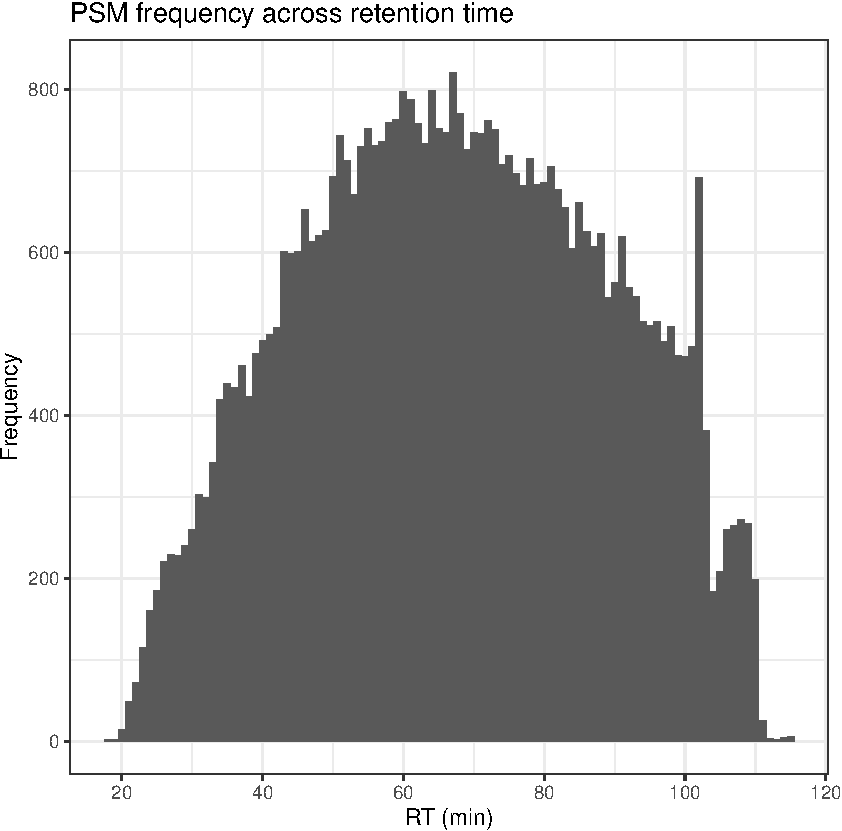
\includegraphics[height=0.3\textheight]{workflow_expressions_files/figure-latex/tmt_RT-1} \end{center}

The four plots that we have generated look relatively standard with no obvious
problems indicated. Therefore, we continue by evaluating the quality of the
processed data.

\subsubsection{Checking the efficiency of TMT labelling}\label{checking-the-efficiency-of-tmt-labelling}

The most fundamental data quality control step in a TMT experiment is to check
the TMT labelling efficiency. TMT labels react with amine groups present at the
peptide N-terminus as well as the side chain of lysine (K) residues. Of note,
lysine residues can be TMT modified regardless of whether they are present at the
C-terminus of a trypic peptide or internally following miscleavage.

To evaluate the TMT labelling efficiency, a separate identification search of the
raw data was completed with lysine (K) and peptide N-termini TMT labels
considered as dynamic modifications rather than static. No additional residues
(S or T) were evaluated for labelling in the search. This allows the search
engine to assess the presence of both the modified (TMT labelled) and unmodified
(original) forms of each peptide. The relative proportions of modified and
unmodified peptides can then be used to calculate the TMT labelling efficiency.
To demonstrate how to check for TMT labelling efficiency, only two of the eight
fractions were utilized for this search.

As we will only look at TMT efficiency at the PSM-level, here we upload the \texttt{.txt}
into a \texttt{data.frame} to format into a \texttt{SummarizedExperiment} object. This is done
using the \texttt{readSummarizedExperiment} function and the same arguments as those
in \texttt{readQFeatures}. The reason for this is that we only need the PSM-level data,
so do not need to generate a \texttt{QFeatures} object with the function of holding
multiple \texttt{SummarizedExperiments} across different levels.

\begin{Shaded}
\begin{Highlighting}[]
\DocumentationTok{\#\# Locate the PSM .txt file}
\NormalTok{tmt\_psm }\OtherTok{\textless{}{-}} \StringTok{"cell\_pellet\_tmt\_efficiency\_psms.txt"}

\DocumentationTok{\#\# Import into a data.frame}
\NormalTok{tmt\_df }\OtherTok{\textless{}{-}} \FunctionTok{read.delim}\NormalTok{(tmt\_psm)}

\DocumentationTok{\#\# Identify columns containing quantitative data}
\NormalTok{tmt\_df }\SpecialCharTok{\%\textgreater{}\%}
  \FunctionTok{names}\NormalTok{()}
\end{Highlighting}
\end{Shaded}

\begin{verbatim}
##  [1] "PSMs.Workflow.ID"                  "PSMs.Peptide.ID"                  
##  [3] "Checked"                           "Tags"                             
##  [5] "Confidence"                        "Identifying.Node.Type"            
##  [7] "Identifying.Node"                  "Search.ID"                        
##  [9] "Identifying.Node.No"               "PSM.Ambiguity"                    
## [11] "Sequence"                          "Annotated.Sequence"               
## [13] "Modifications"                     "Number.of.Proteins"               
## [15] "Master.Protein.Accessions"         "Master.Protein.Descriptions"      
## [17] "Protein.Accessions"                "Protein.Descriptions"             
## [19] "Number.of.Missed.Cleavages"        "Charge"                           
## [21] "Original.Precursor.Charge"         "Delta.Score"                      
## [23] "Delta.Cn"                          "Rank"                             
## [25] "Search.Engine.Rank"                "Concatenated.Rank"                
## [27] "mz.in.Da"                          "MHplus.in.Da"                     
## [29] "Theo.MHplus.in.Da"                 "Delta.M.in.ppm"                   
## [31] "Delta.mz.in.Da"                    "Ions.Matched"                     
## [33] "Matched.Ions"                      "Total.Ions"                       
## [35] "Intensity"                         "Activation.Type"                  
## [37] "NCE.in.Percent"                    "MS.Order"                         
## [39] "Isolation.Interference.in.Percent" "SPS.Mass.Matches.in.Percent"      
## [41] "Average.Reporter.SN"               "Ion.Inject.Time.in.ms"            
## [43] "RT.in.min"                         "First.Scan"                       
## [45] "Last.Scan"                         "Master.Scans"                     
## [47] "Spectrum.File"                     "File.ID"                          
## [49] "Abundance.126"                     "Abundance.127"                    
## [51] "Abundance.128"                     "Abundance.129"                    
## [53] "Abundance.130"                     "Abundance.131"                    
## [55] "Quan.Info"                         "Peptides.Matched"                 
## [57] "XCorr"                             "Number.of.Protein.Groups"         
## [59] "Contaminant"                       "Percolator.q.Value"               
## [61] "Percolator.PEP"                    "Percolator.SVMScore"
\end{verbatim}

\begin{Shaded}
\begin{Highlighting}[]
\DocumentationTok{\#\# Read in as a SummarizedExperiment}
\NormalTok{tmt\_se }\OtherTok{\textless{}{-}} \FunctionTok{readSummarizedExperiment}\NormalTok{(}\AttributeTok{assayData =}\NormalTok{ tmt\_df,}
                                   \AttributeTok{quantCols =} \DecValTok{49}\SpecialCharTok{:}\DecValTok{54}\NormalTok{)}

\DocumentationTok{\#\# Clean sample names}
\FunctionTok{colnames}\NormalTok{(tmt\_se) }\OtherTok{\textless{}{-}} \FunctionTok{c}\NormalTok{(}\StringTok{"S5"}\NormalTok{, }\StringTok{"S2"}\NormalTok{, }\StringTok{"S1"}\NormalTok{, }\StringTok{"S4"}\NormalTok{, }\StringTok{"S6"}\NormalTok{, }\StringTok{"S3"}\NormalTok{)}

\DocumentationTok{\#\# Add sample info as colData to QFeatures object}
\NormalTok{tmt\_se}\SpecialCharTok{$}\NormalTok{label }\OtherTok{\textless{}{-}} \FunctionTok{c}\NormalTok{(}\StringTok{"TMT126"}\NormalTok{,}
                  \StringTok{"TMT127"}\NormalTok{, }
                  \StringTok{"TMT128"}\NormalTok{, }
                  \StringTok{"TMT129"}\NormalTok{,}
                  \StringTok{"TMT130"}\NormalTok{,}
                  \StringTok{"TMT131"}\NormalTok{)}

\NormalTok{tmt\_se}\SpecialCharTok{$}\NormalTok{sample }\OtherTok{\textless{}{-}} \FunctionTok{c}\NormalTok{(}\StringTok{"S5"}\NormalTok{, }\StringTok{"S2"}\NormalTok{, }\StringTok{"S1"}\NormalTok{, }\StringTok{"S4"}\NormalTok{, }\StringTok{"S6"}\NormalTok{, }\StringTok{"S3"}\NormalTok{)}

\NormalTok{tmt\_se}\SpecialCharTok{$}\NormalTok{condition }\OtherTok{\textless{}{-}} \FunctionTok{c}\NormalTok{(}\StringTok{"Control"}\NormalTok{, }\StringTok{"Treated"}\NormalTok{, }\StringTok{"Treated"}\NormalTok{,}
                      \StringTok{"Control"}\NormalTok{, }\StringTok{"Control"}\NormalTok{, }\StringTok{"Treated"}\NormalTok{)}
\end{Highlighting}
\end{Shaded}

\begin{Shaded}
\begin{Highlighting}[]
\DocumentationTok{\#\# Verify}
\FunctionTok{colData}\NormalTok{(tmt\_se)}
\end{Highlighting}
\end{Shaded}

\begin{verbatim}
## DataFrame with 6 rows and 3 columns
##          label      sample   condition
##    <character> <character> <character>
## S5      TMT126          S5     Control
## S2      TMT127          S2     Treated
## S1      TMT128          S1     Treated
## S4      TMT129          S4     Control
## S6      TMT130          S6     Control
## S3      TMT131          S3     Treated
\end{verbatim}

Information about the presence of labels is stored within the `Modifications'
feature of the \texttt{rowData}. Using this information, the TMT labelling efficiency
of the experiment is calculated using the code chunks below. Users should alter
this code if TMTpro reagents are being used such that ``TMT6plex'' is replaced by
``TMTpro''.

First we consider the efficiency of peptide N-termini TMT labelling. We use the
\texttt{grep} function to identify PSMs which are annotated as having an N-Term TMT6plex
modification. We then calculate the number of PSMs with this annotation as a
proportion of the total number of PSMs.

\begin{Shaded}
\begin{Highlighting}[]
\DocumentationTok{\#\# Count the total number of PSMs}
\NormalTok{tmt\_total }\OtherTok{\textless{}{-}} \FunctionTok{length}\NormalTok{(tmt\_se)}

\DocumentationTok{\#\# Count the number of PSMs with an N{-}terminal TMT modification}
\NormalTok{nterm\_labelled\_rows }\OtherTok{\textless{}{-}} \FunctionTok{grep}\NormalTok{(}\StringTok{"N{-}Term}\SpecialCharTok{\textbackslash{}\textbackslash{}}\StringTok{(TMT6plex}\SpecialCharTok{\textbackslash{}\textbackslash{}}\StringTok{)"}\NormalTok{,}
                            \FunctionTok{rowData}\NormalTok{(tmt\_se)}\SpecialCharTok{$}\NormalTok{Modifications)}
\NormalTok{nterm\_psms\_labelled }\OtherTok{\textless{}{-}} \FunctionTok{length}\NormalTok{(nterm\_labelled\_rows)}

\DocumentationTok{\#\# Calculate N{-}terminal TMT labelling efficiency}
\NormalTok{efficiency\_nterm }\OtherTok{\textless{}{-}}\NormalTok{ (nterm\_psms\_labelled }\SpecialCharTok{/}\NormalTok{ tmt\_total) }\SpecialCharTok{*} \DecValTok{100}

\NormalTok{efficiency\_nterm }\SpecialCharTok{\%\textgreater{}\%}
  \FunctionTok{round}\NormalTok{(}\AttributeTok{digits =} \DecValTok{1}\NormalTok{) }\SpecialCharTok{\%\textgreater{}\%}
  \FunctionTok{print}\NormalTok{()}
\end{Highlighting}
\end{Shaded}

\begin{verbatim}
## [1] 96.8
\end{verbatim}

Secondly, we consider the TMT labelling efficiency of lysine (K) residues. As
mentioned above, lysine residues can be TMT labelled regardless of their
position within a peptide. Hence, we here calculate lysine labelling efficiency
on a per lysine residue basis.

\begin{Shaded}
\begin{Highlighting}[]
\DocumentationTok{\#\# Count the number of lysine TMT6plex modifications in the PSM data}
\NormalTok{k\_tmt }\OtherTok{\textless{}{-}} \FunctionTok{str\_count}\NormalTok{(}\AttributeTok{string =} \FunctionTok{rowData}\NormalTok{(tmt\_se)}\SpecialCharTok{$}\NormalTok{Modifications, }
                   \AttributeTok{pattern =} \StringTok{"K[0{-}9]\{1,2\}}\SpecialCharTok{\textbackslash{}\textbackslash{}}\StringTok{(TMT6plex}\SpecialCharTok{\textbackslash{}\textbackslash{}}\StringTok{)"}\NormalTok{) }\SpecialCharTok{\%\textgreater{}\%}
  \FunctionTok{sum}\NormalTok{() }\SpecialCharTok{\%\textgreater{}\%}
  \FunctionTok{as.numeric}\NormalTok{()}

\DocumentationTok{\#\# Count the number of lysine residues in the PSM data}
\NormalTok{k\_total }\OtherTok{\textless{}{-}} \FunctionTok{str\_count}\NormalTok{(}\AttributeTok{string =} \FunctionTok{rowData}\NormalTok{(tmt\_se)}\SpecialCharTok{$}\NormalTok{Sequence, }
                     \AttributeTok{pattern =} \StringTok{"K"}\NormalTok{) }\SpecialCharTok{\%\textgreater{}\%}
  \FunctionTok{sum}\NormalTok{() }\SpecialCharTok{\%\textgreater{}\%}
  \FunctionTok{as.numeric}\NormalTok{()}

\DocumentationTok{\#\# Determine the percentage of TMT labelled lysines}
\NormalTok{efficiency\_k }\OtherTok{\textless{}{-}}\NormalTok{ (k\_tmt }\SpecialCharTok{/}\NormalTok{ k\_total) }\SpecialCharTok{*} \DecValTok{100}

\NormalTok{efficiency\_k }\SpecialCharTok{\%\textgreater{}\%}
  \FunctionTok{round}\NormalTok{(}\AttributeTok{digits =} \DecValTok{1}\NormalTok{) }\SpecialCharTok{\%\textgreater{}\%}
  \FunctionTok{print}\NormalTok{()}
\end{Highlighting}
\end{Shaded}

\begin{verbatim}
## [1] 98.5
\end{verbatim}

Users should aim for an overall TMT labelling efficiency \textgreater90 \% in order to
achieve reliable quantitation. In cases where labelling efficiency is towards
the lower end of the acceptable range, TMT labels should be set as dynamic
modifications during the final identification search, although this will
increase the search space and time as well as influencing FDR calculations. A
summary of the current advice from Thermo Fisher is provided in Table
\ref{tab:table2}. Where labelling efficiency is calculated as being between
categories, how to progress is ultimately decided by the user.

Since the use-case data has a sufficiently high TMT labelling efficiency, we
can continue to use the output of the identification search. This search
considered TMT labelling of lysines as a static modification whilst N-terminal
labelling was kept as dynamic, to investigate the presence of protein N-
terminal modifications.

\begin{table}

\caption{\label{tab:table2}ThermoFisher search strategy recommendations based on TMT labelling efficiency}
\centering
\begin{tabular}[t]{l|l|l}
\hline
N-term efficiency & K efficiency & Suggested search method\\
\hline
> 98 \% & > 98 \% & Both modifications as 'static'\\
\hline
85 - 95 \% & > 98 \% & N-terminal modification 'dynamic' and K modification 'static'\\
\hline
< 84 \% & < 84 \% & Data not suitable for quantitation\\
\hline
\end{tabular}
\end{table}

\subsection{Basic data cleaning}\label{basic-data-cleaning}

Being confident that the experiment and identification search were successful,
we can now begin with some basic data cleaning. However, we also want to keep a
copy of the raw PSM data. Therefore, we first create a second copy of the PSM
\texttt{SummarizedExperiment}, called ``psms\_filtered'', and add it to the \texttt{QFeatures}
object. This is done using the \texttt{addAssay} function. All changes made at the PSM
level will then only be applied to this second copy, so that we can refer back
to the original data if needed.

\begin{Shaded}
\begin{Highlighting}[]
\DocumentationTok{\#\# Extract the "psms\_raw" SummarizedExperiment}
\NormalTok{data\_copy }\OtherTok{\textless{}{-}}\NormalTok{ cp\_qf[[}\StringTok{"psms\_raw"}\NormalTok{]]}

\DocumentationTok{\#\# Add copy of SummarizedExperiment}
\NormalTok{cp\_qf }\OtherTok{\textless{}{-}} \FunctionTok{addAssay}\NormalTok{(}\AttributeTok{x =}\NormalTok{ cp\_qf, }
                  \AttributeTok{y =}\NormalTok{ data\_copy,}
                  \AttributeTok{name =} \StringTok{"psms\_filtered"}\NormalTok{)}

\DocumentationTok{\#\# Verify}
\NormalTok{cp\_qf}
\end{Highlighting}
\end{Shaded}

\begin{verbatim}
## An instance of class QFeatures containing 2 assays:
##  [1] psms_raw: SummarizedExperiment with 48832 rows and 6 columns 
##  [2] psms_filtered: SummarizedExperiment with 48832 rows and 6 columns
\end{verbatim}

Of note, manually adding an assay (or \texttt{SummarizedExperiment}) to the \texttt{QFeatures}
object does not automatically generate links between these assays. We will
manually add the explicit links later, after we complete data cleaning and
filtering.

The cleaning steps included in this section are non-specific and should be applied
to all quantitative proteomics datasets. The names of key parameters will vary in
data outputs from alternative third party software, however, and users should
remain aware of both terminology changes over time as well as the introduction
of new filters. All data cleaning steps are completed in the same way. We first
determine how many rows, here PSMs, meet the conditions for removal. This is
achieved by using the \texttt{dplyr::count} function. The unwanted rows are removed
using the \texttt{filterFeatures} function. Since we only wish to apply the filters to
the ``psms\_filtered'' level, we specify this by using the \texttt{i\ =} argument. If this
argument is not used, \texttt{filterFeatures} will remove features from all assays
within a \texttt{QFeatures} object.

\subsubsection{Removing PSMs not matched to a master protein}\label{removing-psms-not-matched-to-a-master-protein}

The first common cleaning step we carry out is the removal of PSMs that have not
been assigned to a master protein during the identification search. This can
happen when the search software is unable to resolve conflicts caused by the
presence of the isobaric amino acids leucine and isoleucine. Before implementing
the filter, it is useful to find out how many PSMs we expect to remove. This is
easily done by using the \texttt{dplyr::count} on the master protein column. Any master
proteins that return \texttt{TRUE} will be removed by filtering. If this returns
no \texttt{TRUE} values, users should move on to the next filtering step without
removing rows as this will introduce an error.

\begin{Shaded}
\begin{Highlighting}[]
\DocumentationTok{\#\# Find out how many PSMs we expect to lose}
\NormalTok{cp\_qf[[}\StringTok{"psms\_filtered"}\NormalTok{]] }\SpecialCharTok{\%\textgreater{}\%} 
  \FunctionTok{rowData}\NormalTok{() }\SpecialCharTok{\%\textgreater{}\%} 
  \FunctionTok{as\_tibble}\NormalTok{() }\SpecialCharTok{\%\textgreater{}\%} 
\NormalTok{  dplyr}\SpecialCharTok{::}\FunctionTok{count}\NormalTok{(Master.Protein.Accessions }\SpecialCharTok{==} \StringTok{""}\NormalTok{)}
\end{Highlighting}
\end{Shaded}

\begin{verbatim}
## # A tibble: 2 x 2
##   `Master.Protein.Accessions == ""`     n
##   <lgl>                             <int>
## 1 FALSE                             48660
## 2 TRUE                                172
\end{verbatim}

For users who wish to explicitly track the process of data cleaning, the code
chunk below demonstrates how to print a message containing the number of features
removed.

\begin{Shaded}
\begin{Highlighting}[]
\FunctionTok{paste}\NormalTok{(}\StringTok{"Removing"}\NormalTok{, }
      \FunctionTok{length}\NormalTok{(}\FunctionTok{which}\NormalTok{(}\FunctionTok{rowData}\NormalTok{(}
\NormalTok{        cp\_qf[[}\StringTok{"psms\_filtered"}\NormalTok{]])}\SpecialCharTok{$}\NormalTok{Master.Protein.Accessions }\SpecialCharTok{==} \StringTok{""}\NormalTok{)),}
      \StringTok{"PSMs without a master protein accession"}\NormalTok{) }\SpecialCharTok{\%\textgreater{}\%}
  \FunctionTok{message}\NormalTok{()}
\end{Highlighting}
\end{Shaded}

\begin{verbatim}
## Removing 172 PSMs without a master protein accession
\end{verbatim}

This code could be adapted to each cleaning and filtering step. To maintain
simplicity of this workflow, we will not print explicit messages at each step.
Instead, the decision to do so is left to the user.

\begin{Shaded}
\begin{Highlighting}[]
\DocumentationTok{\#\# Remove PSMs without a master protein accession using filterFeatures}
\NormalTok{cp\_qf }\OtherTok{\textless{}{-}}\NormalTok{ cp\_qf }\SpecialCharTok{\%\textgreater{}\%}
  \FunctionTok{filterFeatures}\NormalTok{(}\SpecialCharTok{\textasciitilde{}} \SpecialCharTok{!}\NormalTok{Master.Protein.Accessions }\SpecialCharTok{==} \StringTok{""}\NormalTok{,}
                 \AttributeTok{i =} \StringTok{"psms\_filtered"}\NormalTok{)}
\end{Highlighting}
\end{Shaded}

\subsubsection{Removing PSMs matched to a contaminant protein}\label{removing-psms-matched-to-a-contaminant-protein}

Next we remove PSMs corresponding to contaminant proteins. Such proteins can be
introduced intentionally as reagents during sample preparation, as is the case
for digestive enzymes, or accidentally, as seen with human keratins derived from
skin and hair. Since these proteins do not contribute to the biological question
being asked and it is standard practice to remove them from the data. This is
done by using a carefully curated, sample-specific contaminant database.
Critically, the database used for filtering should be the same one that was used
during the identification search. Whilst it is possible to remove contaminants
using the \texttt{filterFeatures} function on a contaminants annotation column (as per
the \href{https://bioconductor.org/packages/release/bioc/vignettes/QFeatures/inst/doc/Processing.html}{\texttt{QFeatures} processing vignette}),
we demonstrate how to filter using only contaminant protein accessions for users
who do not have contaminant annotations within their identification data.

For this experiment, a contaminant database from \citep{Frankenfield2022} was used.
The \texttt{.fasta} file for this database is available at the \href{Protein\%20Contaminant\%20Libraries\%20for\%20DDA\%20and\%20DIA\%20Proteomics}{Hao Group's Github Repository for Protein Contaminant Libraries for DDA and DIA Proteomics}
and specifically can be found at \url{https://github.com/HaoGroup-ProtContLib/Protein-Contaminant-Libraries-for-DDA-and-DIA-Proteomics/tree/main/Universal\%20protein\%20contaminant\%20FASTA}.
Here, we import this file using the \texttt{fasta.index} function from the
\href{https://bioconductor.org/packages/release/bioc/html/Biostrings.html}{\texttt{Biostrings} package}
\citep{biostrings}. This function requires a file path to the \texttt{.fasta} file and the
asks users to specify the sequence type. In this case we have amino acid
sequences so pass \texttt{seqtype\ =\ "AA"}. The function returns a \texttt{data.frame} with one
row per FASTA entry. We then can extract the protein accessions from the fasta
file. Users will need to alter the below code according to the contaminant file
used.

\begin{Shaded}
\begin{Highlighting}[]
\DocumentationTok{\#\# Load Hao group .fasta file used in search}
\NormalTok{cont\_fasta }\OtherTok{\textless{}{-}} \StringTok{"220813\_universal\_protein\_contaminants\_Haogroup.fasta"}
\NormalTok{conts }\OtherTok{\textless{}{-}}\NormalTok{ Biostrings}\SpecialCharTok{::}\FunctionTok{fasta.index}\NormalTok{(cont\_fasta, }\AttributeTok{seqtype =} \StringTok{"AA"}\NormalTok{)}

\DocumentationTok{\#\# Extract only the protein accessions (not Cont\_ at the start)}
\NormalTok{cont\_acc }\OtherTok{\textless{}{-}} \FunctionTok{regexpr}\NormalTok{(}\StringTok{"(?\textless{}=}\SpecialCharTok{\textbackslash{}\textbackslash{}}\StringTok{\_).*?(?=}\SpecialCharTok{\textbackslash{}\textbackslash{}}\StringTok{|)"}\NormalTok{, conts}\SpecialCharTok{$}\NormalTok{desc, }\AttributeTok{perl =} \ConstantTok{TRUE}\NormalTok{) }\SpecialCharTok{\%\textgreater{}\%}
  \FunctionTok{regmatches}\NormalTok{(conts}\SpecialCharTok{$}\NormalTok{desc, .)}
\end{Highlighting}
\end{Shaded}

Now we have our contaminant list by accession number, we can identify and remove
PSMs with any contaminant protein within their ``Protein.Accessions''.
Importantly, filtering on ``Protein.Accessions'' ensures the removal of PSMs which
matched to a protein group containing a contaminant protein, even if the
contaminant protein is not the group's master protein.

\begin{Shaded}
\begin{Highlighting}[]
\DocumentationTok{\#\# Define function to find contaminants}
\NormalTok{find\_cont }\OtherTok{\textless{}{-}} \ControlFlowTok{function}\NormalTok{(se, cont\_acc) \{}
\NormalTok{  cont\_indices }\OtherTok{\textless{}{-}} \FunctionTok{c}\NormalTok{()}
  \ControlFlowTok{for}\NormalTok{ (i }\ControlFlowTok{in} \DecValTok{1}\SpecialCharTok{:}\FunctionTok{length}\NormalTok{(cont\_acc)) \{}
\NormalTok{    cont\_protein }\OtherTok{\textless{}{-}}\NormalTok{ cont\_acc[i]}
\NormalTok{    cont\_present }\OtherTok{\textless{}{-}} \FunctionTok{grep}\NormalTok{(cont\_protein, }\FunctionTok{rowData}\NormalTok{(se)}\SpecialCharTok{$}\NormalTok{Protein.Accessions)}
\NormalTok{    output }\OtherTok{\textless{}{-}} \FunctionTok{c}\NormalTok{(cont\_present)}
\NormalTok{    cont\_indices }\OtherTok{\textless{}{-}} \FunctionTok{append}\NormalTok{(cont\_indices, output)}
\NormalTok{  \}}
\NormalTok{  cont\_psm\_indices }\OtherTok{\textless{}{-}}\NormalTok{ cont\_indices}
\NormalTok{\}}

\DocumentationTok{\#\# Store row indices of PSMs matched to a contaminant{-}containing protein group}
\NormalTok{cont\_psms }\OtherTok{\textless{}{-}} \FunctionTok{find\_cont}\NormalTok{(cp\_qf[[}\StringTok{"psms\_filtered"}\NormalTok{]], cont\_acc)}

\DocumentationTok{\#\# If we find contaminants, remove these rows from the data}
\ControlFlowTok{if}\NormalTok{ (}\FunctionTok{length}\NormalTok{(cont\_psms) }\SpecialCharTok{\textgreater{}} \DecValTok{0}\NormalTok{)}
\NormalTok{  cp\_qf[[}\StringTok{"psms\_filtered"}\NormalTok{]] }\OtherTok{\textless{}{-}}\NormalTok{ cp\_qf[[}\StringTok{"psms\_filtered"}\NormalTok{]][}\SpecialCharTok{{-}}\NormalTok{cont\_psms, ]}
\end{Highlighting}
\end{Shaded}

At this point, users can also remove any additional proteins which may not have
been included in the contaminant database. For example, users may wish to remove
human trypsin (accession P35050) should it appear in their data.

Several third party software also have the option to directly annotate which
fasta file (here, the human proteome or contaminant database) a PSM is derived
from. In such cases, filtering can be simplified by removing PSMs annotated as
contaminants in the output file.

\subsubsection{Removing PSMs which lack quantitative data}\label{removing-psms-which-lack-quantitative-data}

Now that we are left with only PSMs matched to proteins of interest, we filter
out PSMs which cannot be used for quantitation. This includes some PSMs which
lack quantitative information altogether. In outputs derived from Proteome
Discoverer this information is included in the ``Quan.Info'' column where PSMs are
annotated as having ``NoQuanLabels''. For users who have considered both lysine and
N-terminal TMT labels as static modifications, the data should not contain any
PSMs without quantitative information. However, since the use-case data was
derived from a search in which N-terminal TMT modifications were dynamic, the
data does include this annotation. Users are reminded that column names are
typically software-specific as the ``Quan.Info'' column is found only in outputs
derived from Proteome Discoverer. However, the majority of alternative third
party software will have an equivalent column containing the same information.

\begin{Shaded}
\begin{Highlighting}[]
\DocumentationTok{\#\# Find out how many PSMs we expect to lose}
\NormalTok{cp\_qf[[}\StringTok{"psms\_filtered"}\NormalTok{]] }\SpecialCharTok{\%\textgreater{}\%} 
  \FunctionTok{rowData}\NormalTok{() }\SpecialCharTok{\%\textgreater{}\%} 
  \FunctionTok{as\_tibble}\NormalTok{() }\SpecialCharTok{\%\textgreater{}\%} 
\NormalTok{  dplyr}\SpecialCharTok{::}\FunctionTok{count}\NormalTok{(Quan.Info }\SpecialCharTok{==} \StringTok{"NoQuanLabels"}\NormalTok{)}
\end{Highlighting}
\end{Shaded}

\begin{verbatim}
## # A tibble: 2 x 2
##   `Quan.Info == "NoQuanLabels"`     n
##   <lgl>                         <int>
## 1 FALSE                         47241
## 2 TRUE                            228
\end{verbatim}

\begin{Shaded}
\begin{Highlighting}[]
\DocumentationTok{\#\# Drop these rows from the data}
\NormalTok{cp\_qf }\OtherTok{\textless{}{-}}\NormalTok{ cp\_qf }\SpecialCharTok{\%\textgreater{}\%}
  \FunctionTok{filterFeatures}\NormalTok{(}\SpecialCharTok{\textasciitilde{}} \SpecialCharTok{!}\NormalTok{Quan.Info }\SpecialCharTok{==} \StringTok{"NoQuanLabels"}\NormalTok{, }
                 \AttributeTok{i =} \StringTok{"psms\_filtered"}\NormalTok{)}
\end{Highlighting}
\end{Shaded}

This point in the workflow is a good time to check whether there are any other
annotations within the ``Quan.Info'' column. For example, if there are any PSMs
which have been ``ExcludedByMethod'', this indicates that a PSM-level filter was
applied in Proteome Discoverer during the identification search. If this is the
case, users should determine which filter has been applied to the data and
decide whether to remove the PSMs which were ``ExcludedByMethod'' (thereby applying
the pre-set threshold) or leave them in (disregard the threshold).

\begin{Shaded}
\begin{Highlighting}[]
\DocumentationTok{\#\# Are there any remaining annotations in the Quan.Info column?}
\NormalTok{cp\_qf[[}\StringTok{"psms\_filtered"}\NormalTok{]] }\SpecialCharTok{\%\textgreater{}\%} 
  \FunctionTok{rowData}\NormalTok{() }\SpecialCharTok{\%\textgreater{}\%} 
  \FunctionTok{as\_tibble}\NormalTok{() }\SpecialCharTok{\%\textgreater{}\%} 
  \FunctionTok{pull}\NormalTok{(Quan.Info) }\SpecialCharTok{\%\textgreater{}\%} 
  \FunctionTok{table}\NormalTok{()}
\end{Highlighting}
\end{Shaded}

\begin{verbatim}
## .
##       
## 47241
\end{verbatim}

In the above code chunk we see there are no remaining annotations in the
``Quan.Info'' column so we can continue.

\subsubsection{Removing PSMs which are not unique to a protein}\label{removing-psms-which-are-not-unique-to-a-protein}

The next step is to consider which PSMs are to be used for quantitation. There
are two ways in which a PSM can be considered as unique. The first and most pure
form of uniqueness comes from a PSM corresponding to a single protein only. This
results in the PSM being allocated to one protein and one protein group.
However, it is common to expand the definition of unique to include PSMs that
map to multiple proteins within a single protein group. That is PSMs which are
allocated to more than one protein but only one protein group. This distinction
is ultimately up to the user. By contrast, PSMs corresponding to razor and
shared peptides are linked to multiple proteins across multiple protein groups.
In this workflow, the final grouping of peptides to proteins will be done based
on master protein accession. Therefore, differential expression analysis will be
based on protein groups, and we here consider unique as any PSM linked to only
one protein group. This means removing PSMs where ``Number.of.Protein.Groups'' is
not equal to 1.

In the below code chunk we count the number of PSMs linked to more than 1
protein group.

\begin{Shaded}
\begin{Highlighting}[]
\DocumentationTok{\#\# Find out how many PSMs we expect to lose}
\NormalTok{cp\_qf[[}\StringTok{"psms\_filtered"}\NormalTok{]] }\SpecialCharTok{\%\textgreater{}\%} 
  \FunctionTok{rowData}\NormalTok{() }\SpecialCharTok{\%\textgreater{}\%} 
  \FunctionTok{as\_tibble}\NormalTok{() }\SpecialCharTok{\%\textgreater{}\%} 
\NormalTok{  dplyr}\SpecialCharTok{::}\FunctionTok{count}\NormalTok{(Number.of.Protein.Groups }\SpecialCharTok{!=} \DecValTok{1}\NormalTok{)}
\end{Highlighting}
\end{Shaded}

\begin{verbatim}
## # A tibble: 2 x 2
##   `Number.of.Protein.Groups != 1`     n
##   <lgl>                           <int>
## 1 FALSE                           44501
## 2 TRUE                             2740
\end{verbatim}

We again use the \texttt{filterFeatures} function to retain PSMs linked to only
1 protein group and discard any PSMs linked to more 1 group.

\begin{Shaded}
\begin{Highlighting}[]
\DocumentationTok{\#\# Remove these rows from the data}
\NormalTok{cp\_qf }\OtherTok{\textless{}{-}}\NormalTok{ cp\_qf }\SpecialCharTok{\%\textgreater{}\%}
  \FunctionTok{filterFeatures}\NormalTok{(}\SpecialCharTok{\textasciitilde{}}\NormalTok{ Number.of.Protein.Groups }\SpecialCharTok{==} \DecValTok{1}\NormalTok{, }
                 \AttributeTok{i =} \StringTok{"psms\_filtered"}\NormalTok{)}
\end{Highlighting}
\end{Shaded}

\paragraph{Additional considerations regarding protein isoforms}\label{additional-considerations-regarding-protein-isoforms}

Users searching against a database that includes protein isoforms must take
extra caution when defining `unique' PSMs. A PSM that corresponds to a single
protein when data is searched against the proteome without isoforms may
correspond to multiple proteins once additional isoforms are included. As a
result, PSMs or peptides that were previously mapped to one protein and one
protein group could instead be mapped to multiple proteins and one protein group.
These PSMs would be filtered out by defining `unique' as corresponding to only
one protein and one protein group, but would be retained if the definition was
expanded to multiple proteins and one protein group. Users should be aware of
these possibilities and select their filtering strategy based on the biological
question of interest.

\subsubsection{Removing PSMs that are not rank 1}\label{removing-psms-that-are-not-rank-1}

Another filter that is important for quantitation is that of PSM rank. Since
individual spectra can have multiple candidate peptide matches, Proteome
Discoverer uses a scoring algorithm to determine the probability of a PSM being
incorrect. Once each candidate PSM has been given a score, the one with the
lowest score (lowest probability of being incorrect) is allocated rank 1. The PSM
with the second lowest probability of being incorrect is rank 2, and so on. For
the analysis, we only want rank 1 PSMs to be retained.

\begin{Shaded}
\begin{Highlighting}[]
\DocumentationTok{\#\# Find out how many PSMs we expect to lose}
\NormalTok{cp\_qf[[}\StringTok{"psms\_filtered"}\NormalTok{]] }\SpecialCharTok{\%\textgreater{}\%} 
  \FunctionTok{rowData}\NormalTok{() }\SpecialCharTok{\%\textgreater{}\%} 
  \FunctionTok{as\_tibble}\NormalTok{() }\SpecialCharTok{\%\textgreater{}\%} 
\NormalTok{  dplyr}\SpecialCharTok{::}\FunctionTok{count}\NormalTok{(Rank }\SpecialCharTok{!=} \DecValTok{1}\NormalTok{)}
\end{Highlighting}
\end{Shaded}

\begin{verbatim}
## # A tibble: 2 x 2
##   `Rank != 1`     n
##   <lgl>       <int>
## 1 FALSE       43426
## 2 TRUE         1075
\end{verbatim}

\begin{Shaded}
\begin{Highlighting}[]
\DocumentationTok{\#\# Drop these rows from the data}
\NormalTok{cp\_qf }\OtherTok{\textless{}{-}}\NormalTok{ cp\_qf }\SpecialCharTok{\%\textgreater{}\%}
  \FunctionTok{filterFeatures}\NormalTok{(}\SpecialCharTok{\textasciitilde{}}\NormalTok{ Rank }\SpecialCharTok{==} \DecValTok{1}\NormalTok{,}
                 \AttributeTok{i =} \StringTok{"psms\_filtered"}\NormalTok{)}
\end{Highlighting}
\end{Shaded}

The majority of search engines, including SequestHT, also provide their own PSM
rank. To be conservative and ensure accurate quantitation, we also only retain
PSMs that have a search engine rank of 1.

\begin{Shaded}
\begin{Highlighting}[]
\DocumentationTok{\#\# Find out how many PSMs we expect to lose}
\NormalTok{cp\_qf[[}\StringTok{"psms\_filtered"}\NormalTok{]] }\SpecialCharTok{\%\textgreater{}\%} 
  \FunctionTok{rowData}\NormalTok{() }\SpecialCharTok{\%\textgreater{}\%} 
  \FunctionTok{as\_tibble}\NormalTok{() }\SpecialCharTok{\%\textgreater{}\%} 
\NormalTok{  dplyr}\SpecialCharTok{::}\FunctionTok{count}\NormalTok{(Search.Engine.Rank }\SpecialCharTok{!=} \DecValTok{1}\NormalTok{)}
\end{Highlighting}
\end{Shaded}

\begin{verbatim}
## # A tibble: 2 x 2
##   `Search.Engine.Rank != 1`     n
##   <lgl>                     <int>
## 1 FALSE                     43153
## 2 TRUE                        273
\end{verbatim}

\begin{Shaded}
\begin{Highlighting}[]
\DocumentationTok{\#\# Drop these rows from the data}
\NormalTok{cp\_qf }\OtherTok{\textless{}{-}}\NormalTok{ cp\_qf }\SpecialCharTok{\%\textgreater{}\%}
  \FunctionTok{filterFeatures}\NormalTok{(}\SpecialCharTok{\textasciitilde{}}\NormalTok{ Search.Engine.Rank }\SpecialCharTok{==} \DecValTok{1}\NormalTok{,}
                 \AttributeTok{i =} \StringTok{"psms\_filtered"}\NormalTok{)}
\end{Highlighting}
\end{Shaded}

\subsubsection{Removing ambiguous PSMs}\label{removing-ambiguous-psms}

We also retain only unambiguous PSMs. Since there are several candidate
peptides for each spectra, Proteome Discoverer allocates each PSM a level of
ambiguity to indicate whether it was possible to determine a definite PSM or
whether one had to be selected from a number of candidates. The allocation of
PSM ambiguity takes place during the process of protein grouping and the
definitions of each ambiguity assignment are given below in Table
\ref{tab:table3}.

\begin{table}

\caption{\label{tab:table3}Definitions of PSM ambiguity categories based on Proteome Discoverer outputs.}
\centering
\begin{tabular}[t]{l|l}
\hline
PSM category & Definition\\
\hline
Unambiguous & The only candidate PSM\\
\hline
Selected & PSM was selected from a group of candidates\\
\hline
Rejected & PSM was rejected from a group of candidates\\
\hline
Ambiguous & Two or more candidate PSMs could not be distinguished\\
\hline
Unconsidered & PSM was not considered suitable\\
\hline
\end{tabular}
\end{table}

Importantly, depending upon the software being used, output files may already
have excluded some of these categories. It is still good to check before
proceeding with the data.

\begin{Shaded}
\begin{Highlighting}[]
\DocumentationTok{\#\# Find out how many PSMs we expect to lose}
\NormalTok{cp\_qf[[}\StringTok{"psms\_filtered"}\NormalTok{]] }\SpecialCharTok{\%\textgreater{}\%} 
  \FunctionTok{rowData}\NormalTok{() }\SpecialCharTok{\%\textgreater{}\%} 
  \FunctionTok{as\_tibble}\NormalTok{() }\SpecialCharTok{\%\textgreater{}\%} 
\NormalTok{  dplyr}\SpecialCharTok{::}\FunctionTok{count}\NormalTok{(PSM.Ambiguity }\SpecialCharTok{!=} \StringTok{"Unambiguous"}\NormalTok{)}
\end{Highlighting}
\end{Shaded}

\begin{verbatim}
## # A tibble: 1 x 2
##   `PSM.Ambiguity != "Unambiguous"`     n
##   <lgl>                            <int>
## 1 FALSE                            43153
\end{verbatim}

\begin{Shaded}
\begin{Highlighting}[]
\DocumentationTok{\#\# No PSMs to remove so proceed}
\end{Highlighting}
\end{Shaded}

\subsubsection{Controlling false discovery rate}\label{controlling-false-discovery-rate}

Finally, it is necessary to control the false discovery rate. During a database
search, peptide spectrum matches (PSMs) are generated by matching raw mass spectra
to peptide sequences. However, only a number of these PSMs will be true positive
matches, whilst the rest are false positives, or `false discoveries'. Most third
party software contain internal algorithms to determine the number of false
discoveries and the probability of a given feature (PSM, peptide or protein)
being a false discovery. This information can then be used to control the false
discovery rate (FDR), typically to keep this below 5\% for exploratory analyses or
1\% for stringent analyses.

During the database search of the use-case data, only high confidence PSMs with
an FDR \textless{} 1\% were retained.

\begin{Shaded}
\begin{Highlighting}[]
\NormalTok{cp\_qf[[}\StringTok{"psms\_filtered"}\NormalTok{]] }\SpecialCharTok{\%\textgreater{}\%}
  \FunctionTok{rowData}\NormalTok{() }\SpecialCharTok{\%\textgreater{}\%}
  \FunctionTok{as\_tibble}\NormalTok{() }\SpecialCharTok{\%\textgreater{}\%}
  \FunctionTok{pull}\NormalTok{(Confidence) }\SpecialCharTok{\%\textgreater{}\%}
  \FunctionTok{table}\NormalTok{()}
\end{Highlighting}
\end{Shaded}

\begin{verbatim}
## .
##  High 
## 43153
\end{verbatim}

Importantly, however, FDR becomes inflated as you aggregate up from PSM to
peptide and then from peptide to protein. Therefore, a 1\% FDR at PSM-level does
not ensure a 1\% FDR at protein-level. To access information about protein-level
FDR, we have to import the protein-level \texttt{.txt} file from our database search.
As before, users should store this file in their working directory.

\begin{Shaded}
\begin{Highlighting}[]
\DocumentationTok{\#\# Import protein{-}level data}
\NormalTok{protein\_cp }\OtherTok{\textless{}{-}} \FunctionTok{read.delim}\NormalTok{(}\AttributeTok{file =} \StringTok{"cell\_pellet\_tmt\_results\_proteins.txt"}\NormalTok{)}

\DocumentationTok{\#\# Check column names}
\NormalTok{protein\_cp }\SpecialCharTok{\%\textgreater{}\%}
  \FunctionTok{names}\NormalTok{()}
\end{Highlighting}
\end{Shaded}

\begin{verbatim}
##  [1] "Proteins.Unique.Sequence.ID"                    
##  [2] "Checked"                                        
##  [3] "Tags"                                           
##  [4] "Protein.FDR.Confidence.Combined"                
##  [5] "Master"                                         
##  [6] "Protein.Group.IDs"                              
##  [7] "Accession"                                      
##  [8] "Description"                                    
##  [9] "Sequence"                                       
## [10] "FASTA.Title.Lines"                              
## [11] "Exp.q.value.Combined"                           
## [12] "Sum.PEP.Score"                                  
## [13] "Number.of.Decoy.Protein.Combined"               
## [14] "Coverage.in.Percent"                            
## [15] "Number.of.Peptides"                             
## [16] "Number.of.PSMs"                                 
## [17] "Number.of.Protein.Unique.Peptides"              
## [18] "Number.of.Unique.Peptides"                      
## [19] "Number.of.AAs"                                  
## [20] "MW.in.kDa"                                      
## [21] "calc.pI"                                        
## [22] "Score.Sequest.HT.Sequest.HT"                    
## [23] "Coverage.in.Percent.by.Search.Engine.Sequest.HT"
## [24] "Number.of.PSMs.by.Search.Engine.Sequest.HT"     
## [25] "Number.of.Peptides.by.Search.Engine.Sequest.HT" 
## [26] "Abundance.F1.126.Sample"                        
## [27] "Abundance.F1.127.Sample"                        
## [28] "Abundance.F1.128.Sample"                        
## [29] "Abundance.F1.129.Sample"                        
## [30] "Abundance.F1.130.Sample"                        
## [31] "Abundance.F1.131.Sample"                        
## [32] "Abundances.Count.F1.126.Sample"                 
## [33] "Abundances.Count.F1.127.Sample"                 
## [34] "Abundances.Count.F1.128.Sample"                 
## [35] "Abundances.Count.F1.129.Sample"                 
## [36] "Abundances.Count.F1.130.Sample"                 
## [37] "Abundances.Count.F1.131.Sample"                 
## [38] "Found.in.Fraction.F11"                          
## [39] "Found.in.Fraction.F12"                          
## [40] "Found.in.Fraction.F13"                          
## [41] "Found.in.Fraction.F14"                          
## [42] "Found.in.Fraction.F15"                          
## [43] "Found.in.Fraction.F16"                          
## [44] "Found.in.Fraction.F17"                          
## [45] "Found.in.Fraction.F18"                          
## [46] "Found.in.Sample.in.S1.F1.126.Sample"            
## [47] "Found.in.Sample.in.S2.F1.127.Sample"            
## [48] "Found.in.Sample.in.S3.F1.128.Sample"            
## [49] "Found.in.Sample.in.S4.F1.129.Sample"            
## [50] "Found.in.Sample.in.S5.F1.130.Sample"            
## [51] "Found.in.Sample.in.S6.F1.131.Sample"            
## [52] "Found.in.Sample.Group.in.S1.F1.126.Sample"      
## [53] "Found.in.Sample.Group.in.S2.F1.127.Sample"      
## [54] "Found.in.Sample.Group.in.S3.F1.128.Sample"      
## [55] "Found.in.Sample.Group.in.S4.F1.129.Sample"      
## [56] "Found.in.Sample.Group.in.S5.F1.130.Sample"      
## [57] "Found.in.Sample.Group.in.S6.F1.131.Sample"      
## [58] "Number.of.Protein.Groups"
\end{verbatim}

The FDR information is contained in a column called \texttt{Protein.FDR.Confidence.Combined}.
We can get an overview of the data in this column by using the \texttt{table} function.

\begin{Shaded}
\begin{Highlighting}[]
\NormalTok{protein\_cp }\SpecialCharTok{\%\textgreater{}\%}
  \FunctionTok{pull}\NormalTok{(Protein.FDR.Confidence.Combined) }\SpecialCharTok{\%\textgreater{}\%}
  \FunctionTok{table}\NormalTok{()}
\end{Highlighting}
\end{Shaded}

\begin{verbatim}
## .
##   High    Low Medium 
##   4824     75    467
\end{verbatim}

We see proteins that are annotated as high confidence = FDR \textless{} 1\%, medium
confidence = FDR \textless{} 5\% and low confidence = FDR \textgreater{} 5\%.

In order to use the \texttt{filterFeatures} function to remove PSMs corresponding to
proteins which do not pass our FDR threshold (1\%), we first need to add this
annotation to the \texttt{rowData} of our \texttt{"psms\_filtered"} experiment. To do this, we
first extract the master protein accessions from our PSM-level data. Next, we
extract these proteins from our protein-level search output along with their
corresponding confidence ratings.

\begin{Shaded}
\begin{Highlighting}[]
\DocumentationTok{\#\# Extract master protein accessions from our PSM{-}level data}
\NormalTok{proteins\_in\_data }\OtherTok{\textless{}{-}}\NormalTok{ cp\_qf[[}\StringTok{"psms\_filtered"}\NormalTok{]] }\SpecialCharTok{\%\textgreater{}\%}
  \FunctionTok{rowData}\NormalTok{() }\SpecialCharTok{\%\textgreater{}\%}
  \FunctionTok{as\_tibble}\NormalTok{() }\SpecialCharTok{\%\textgreater{}\%}
  \FunctionTok{select}\NormalTok{(Master.Protein.Accessions)}

\DocumentationTok{\#\# Extract protein accessions and corresponding confidence from search output file}
\NormalTok{protein\_search\_output }\OtherTok{\textless{}{-}}\NormalTok{ protein\_cp }\SpecialCharTok{\%\textgreater{}\%}
  \FunctionTok{select}\NormalTok{(Accession, Protein.FDR.Confidence.Combined)}
\end{Highlighting}
\end{Shaded}

Now we can use the \texttt{left\_join} function to merge these two datasets.

\begin{Shaded}
\begin{Highlighting}[]
\DocumentationTok{\#\# Combine data}
\NormalTok{protein\_fdr }\OtherTok{\textless{}{-}} \FunctionTok{left\_join}\NormalTok{(}\AttributeTok{x =}\NormalTok{ proteins\_in\_data, }
                         \AttributeTok{y =}\NormalTok{ protein\_search\_output, }
                         \AttributeTok{by =} \FunctionTok{c}\NormalTok{(}\StringTok{"Master.Protein.Accessions"} \OtherTok{=} \StringTok{"Accession"}\NormalTok{))}

\NormalTok{protein\_fdr }\SpecialCharTok{\%\textgreater{}\%}
  \FunctionTok{head}\NormalTok{()}
\end{Highlighting}
\end{Shaded}

\begin{verbatim}
## # A tibble: 6 x 2
##   Master.Protein.Accessions Protein.FDR.Confidence.Combined
##   <chr>                     <chr>                          
## 1 Q92597                    High                           
## 2 Q9UGP4                    High                           
## 3 Q9BRX2                    High                           
## 4 P14868                    High                           
## 5 O00154                    High                           
## 6 P48651                    High
\end{verbatim}

Finally, we add the annotations from our \texttt{"Protein.FDR.Confidence.Combined"}
column to the \texttt{rowData} of our \texttt{"psms\_filtered"} experiment.

\begin{Shaded}
\begin{Highlighting}[]
\FunctionTok{rowData}\NormalTok{(cp\_qf[[}\StringTok{"psms\_filtered"}\NormalTok{]])}\SpecialCharTok{$}\NormalTok{Protein.Confidence }\OtherTok{\textless{}{-}}\NormalTok{ protein\_fdr}\SpecialCharTok{$}\NormalTok{Protein.FDR.Confidence.Combined}
\end{Highlighting}
\end{Shaded}

We can now use \texttt{filterFeatures} to remove PSMs corresponding to low or medium
confidence master proteins.

\begin{Shaded}
\begin{Highlighting}[]
\NormalTok{cp\_qf }\OtherTok{\textless{}{-}}\NormalTok{ cp\_qf }\SpecialCharTok{\%\textgreater{}\%}
  \FunctionTok{filterFeatures}\NormalTok{(}\SpecialCharTok{\textasciitilde{}}\NormalTok{ Protein.Confidence }\SpecialCharTok{==} \StringTok{"High"}\NormalTok{, }\AttributeTok{i =} \StringTok{"psms\_filtered"}\NormalTok{)}
\end{Highlighting}
\end{Shaded}

\begin{verbatim}
## 'Protein.Confidence' found in 1 out of 2 assay(s)
## No filter applied to the following assay(s) because one or more filtering variables are missing in the rowData: psms_raw.
## You can control whether to remove or keep the features using the 'keep' argument (see '?filterFeature').
\end{verbatim}

\subsubsection{Assessing the impact of non-specific data cleaning}\label{assessing-the-impact-of-non-specific-data-cleaning}

Now that we have finished the non-specific data cleaning, we can pause and check
to see what this has done to the data. We determine the number and proportion of
PSMs, peptides, and proteins lost from the original dataset.

\begin{Shaded}
\begin{Highlighting}[]
\DocumentationTok{\#\# Determine number and proportion of PSMs removed}
\NormalTok{psms\_remaining }\OtherTok{\textless{}{-}}\NormalTok{ cp\_qf[[}\StringTok{"psms\_filtered"}\NormalTok{]] }\SpecialCharTok{\%\textgreater{}\%}
  \FunctionTok{nrow}\NormalTok{() }\SpecialCharTok{\%\textgreater{}\%}
  \FunctionTok{as.numeric}\NormalTok{()}

\NormalTok{psms\_removed }\OtherTok{\textless{}{-}}\NormalTok{ original\_psms }\SpecialCharTok{{-}}\NormalTok{ psms\_remaining}
\NormalTok{psms\_removed\_prop }\OtherTok{\textless{}{-}}\NormalTok{ ((psms\_removed }\SpecialCharTok{/}\NormalTok{ original\_psms) }\SpecialCharTok{*} \DecValTok{100}\NormalTok{) }\SpecialCharTok{\%\textgreater{}\%}
  \FunctionTok{round}\NormalTok{(}\AttributeTok{digits =} \DecValTok{2}\NormalTok{)}

\DocumentationTok{\#\# Determine number and proportion of peptides removed}
\NormalTok{peps\_remaining }\OtherTok{\textless{}{-}}\NormalTok{ cp\_qf[[}\StringTok{"psms\_filtered"}\NormalTok{]] }\SpecialCharTok{\%\textgreater{}\%}
  \FunctionTok{rowData}\NormalTok{() }\SpecialCharTok{\%\textgreater{}\%} 
  \FunctionTok{as\_tibble}\NormalTok{() }\SpecialCharTok{\%\textgreater{}\%} 
  \FunctionTok{pull}\NormalTok{(Sequence) }\SpecialCharTok{\%\textgreater{}\%} 
  \FunctionTok{unique}\NormalTok{() }\SpecialCharTok{\%\textgreater{}\%}
  \FunctionTok{length}\NormalTok{() }\SpecialCharTok{\%\textgreater{}\%}
  \FunctionTok{as.numeric}\NormalTok{()}

\NormalTok{peps\_removed }\OtherTok{\textless{}{-}}\NormalTok{ original\_peps }\SpecialCharTok{{-}}\NormalTok{ peps\_remaining}
\NormalTok{peps\_removed\_prop }\OtherTok{\textless{}{-}}\NormalTok{ ((peps\_removed }\SpecialCharTok{/}\NormalTok{ original\_peps) }\SpecialCharTok{*} \DecValTok{100}\NormalTok{) }\SpecialCharTok{\%\textgreater{}\%}
  \FunctionTok{round}\NormalTok{(}\AttributeTok{digits =} \DecValTok{2}\NormalTok{)}

\DocumentationTok{\#\# Determine number and proportion of proteins removed}
\NormalTok{prots\_remaining }\OtherTok{\textless{}{-}}\NormalTok{ cp\_qf[[}\StringTok{"psms\_filtered"}\NormalTok{]] }\SpecialCharTok{\%\textgreater{}\%} 
  \FunctionTok{rowData}\NormalTok{() }\SpecialCharTok{\%\textgreater{}\%} 
  \FunctionTok{as\_tibble}\NormalTok{() }\SpecialCharTok{\%\textgreater{}\%} 
  \FunctionTok{pull}\NormalTok{(Master.Protein.Accessions) }\SpecialCharTok{\%\textgreater{}\%} 
  \FunctionTok{unique}\NormalTok{() }\SpecialCharTok{\%\textgreater{}\%}
  \FunctionTok{length}\NormalTok{() }\SpecialCharTok{\%\textgreater{}\%}
  \FunctionTok{as.numeric}\NormalTok{() }

\NormalTok{prots\_removed }\OtherTok{\textless{}{-}}\NormalTok{ original\_prots }\SpecialCharTok{{-}}\NormalTok{ prots\_remaining}
\NormalTok{prots\_removed\_prop }\OtherTok{\textless{}{-}}\NormalTok{ ((prots\_removed }\SpecialCharTok{/}\NormalTok{ original\_prots) }\SpecialCharTok{*} \DecValTok{100}\NormalTok{) }\SpecialCharTok{\%\textgreater{}\%}
  \FunctionTok{round}\NormalTok{(}\AttributeTok{digits =} \DecValTok{2}\NormalTok{)}
\end{Highlighting}
\end{Shaded}

\begin{Shaded}
\begin{Highlighting}[]
\DocumentationTok{\#\# Print as a table}
\FunctionTok{data.frame}\NormalTok{(}\StringTok{"Feature"} \OtherTok{=} \FunctionTok{c}\NormalTok{(}\StringTok{"PSMs"}\NormalTok{,}
                         \StringTok{"Peptides"}\NormalTok{,}
                         \StringTok{"Proteins"}\NormalTok{),}
           \StringTok{"Number lost"} \OtherTok{=} \FunctionTok{c}\NormalTok{(psms\_removed,}
\NormalTok{                             peps\_removed,}
\NormalTok{                             prots\_removed),}
           \StringTok{"Percentage lost"} \OtherTok{=} \FunctionTok{c}\NormalTok{(psms\_removed\_prop,}
\NormalTok{                                 peps\_removed\_prop,}
\NormalTok{                                 prots\_removed\_prop))}
\end{Highlighting}
\end{Shaded}

\begin{verbatim}
##    Feature Number.lost Percentage.lost
## 1     PSMs        6066           12.42
## 2 Peptides        1925            7.41
## 3 Proteins         812           16.11
\end{verbatim}

\subsection{PSM quality control filtering}\label{psm-quality-control-filtering}

The next step is to take a look at the data and make informed decisions about
in-depth filtering. Here, we focus on three key quality control filters for TMT
data: 1) average reporter ion signal-to-noise (S/N) ratio, 2) percentage
co-isolation interference, and 3) percentage SPS mass match. It is possible to
set thresholds for these three parameters during the identification search.
However, specifying thresholds prior to exploring the data could lead to
unnecessarily excessive data exclusion or the retention of poor quality PSMs. We
suggest that users set the thresholds for all three aforementioned filters to 0
during the identification search, thus allowing maximum flexibility during data
processing. In all cases, quality control filtering represents a trade-off
between ensuring high quality data and losing potentially informative data. This
means that the thresholds used for such filtering will likely depend upon the
initial quality of the data and the number of PSMs, as well as the experimental
goal being stringent or exploratory.

\subsubsection{Quality control: Average reporter ion signal-to-noise}\label{quality-control-average-reporter-ion-signal-to-noise}

Intensity measurements derived from a small number of ions tend to be more
variable and less accurate. Therefore, reporter ion spectra with peaks generated
from a small number of ions should be filtered out to ensure accurate
quantitation and avoid stochastic ion effects. When using an orbitrap analyzer,
as was the case in the collection of the use-case data, the number of ions is
proportional to the S/N value of a peak. Hence, the average reporter ion S/N
ratio can be used to filter out quantification based on too few ions.

To determine an appropriate reporter ion S/N threshold we need to understand the
original, unfiltered data. Here, we print a \texttt{summary} of the average reporter
S/N before plotting a simple histogram to visualize the data. The default
threshold for average reporter ion S/N when filtering within Proteome Discoverer
is 10, or 1 on the base-10 logarithmic scale displayed here. We include a line
to show where this threshold would be on the data distribution.

\begin{Shaded}
\begin{Highlighting}[]
\DocumentationTok{\#\# Get summary information}
\NormalTok{cp\_qf[[}\StringTok{"psms\_filtered"}\NormalTok{]] }\SpecialCharTok{\%\textgreater{}\%} 
  \FunctionTok{rowData}\NormalTok{() }\SpecialCharTok{\%\textgreater{}\%} 
  \FunctionTok{as\_tibble}\NormalTok{() }\SpecialCharTok{\%\textgreater{}\%} 
  \FunctionTok{pull}\NormalTok{(Average.Reporter.SN) }\SpecialCharTok{\%\textgreater{}\%} 
  \FunctionTok{summary}\NormalTok{()}
\end{Highlighting}
\end{Shaded}

\begin{verbatim}
##    Min. 1st Qu.  Median    Mean 3rd Qu.    Max.    NA's 
##     0.3    84.3   216.4   322.1   451.1  3008.2     138
\end{verbatim}

\begin{Shaded}
\begin{Highlighting}[]
\DocumentationTok{\#\# Plot histogram of reporter ion signal{-}to{-}noise}
\NormalTok{cp\_qf[[}\StringTok{"psms\_filtered"}\NormalTok{]] }\SpecialCharTok{\%\textgreater{}\%} 
  \FunctionTok{rowData}\NormalTok{() }\SpecialCharTok{\%\textgreater{}\%} 
  \FunctionTok{as\_tibble}\NormalTok{() }\SpecialCharTok{\%\textgreater{}\%}
  \FunctionTok{ggplot}\NormalTok{(}\FunctionTok{aes}\NormalTok{(}\AttributeTok{x =} \FunctionTok{log10}\NormalTok{(Average.Reporter.SN))) }\SpecialCharTok{+}
  \FunctionTok{geom\_histogram}\NormalTok{(}\AttributeTok{binwidth =} \FloatTok{0.05}\NormalTok{) }\SpecialCharTok{+}
  \FunctionTok{geom\_vline}\NormalTok{(}\AttributeTok{xintercept =} \DecValTok{1}\NormalTok{, }\AttributeTok{linetype =} \StringTok{"dashed"}\NormalTok{, }\AttributeTok{color =} \StringTok{"red"}\NormalTok{) }\SpecialCharTok{+}
  \FunctionTok{labs}\NormalTok{(}\AttributeTok{x =} \StringTok{"log10(average reporter SN)"}\NormalTok{, }\AttributeTok{y =} \StringTok{"Frequency"}\NormalTok{) }\SpecialCharTok{+}
  \FunctionTok{ggtitle}\NormalTok{(}\StringTok{"Average reporter ion S/N"}\NormalTok{) }\SpecialCharTok{+}
  \FunctionTok{theme\_bw}\NormalTok{()}
\end{Highlighting}
\end{Shaded}

\begin{center}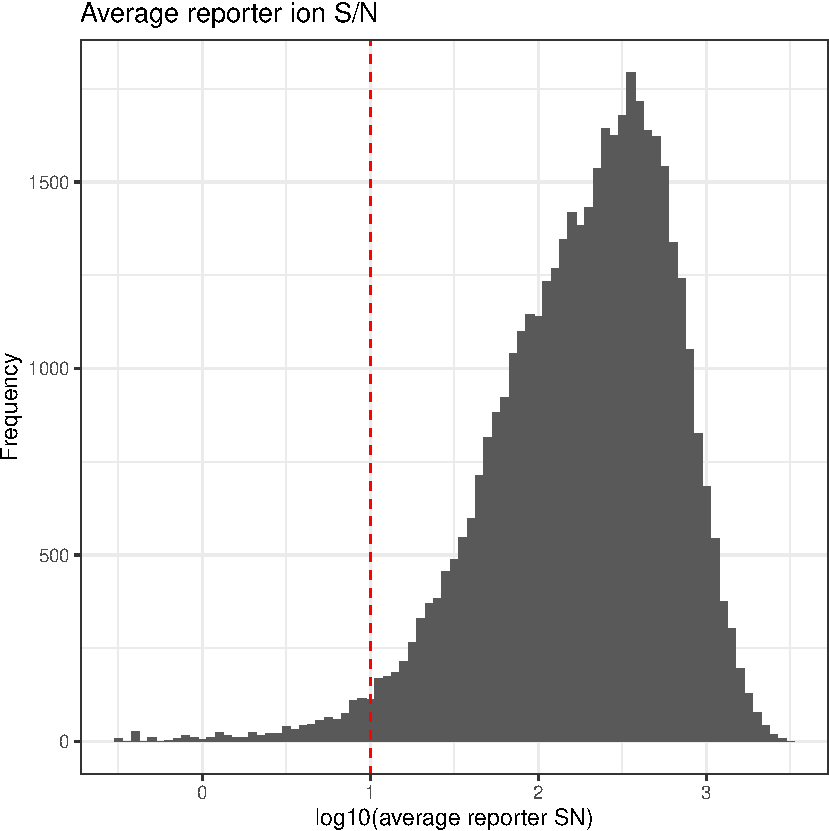
\includegraphics[height=0.3\textheight]{workflow_expressions_files/figure-latex/tmt_sn_ratio_2-1} \end{center}

From the distribution of the data it is clear that applying such a threshold
would not result in dramatic data loss. Whilst we could set a higher threshold
for more stringent analysis, this would lead to unnecessary data loss.
Therefore, we keep PSMs with an average reporter ion S/N threshold of 10 or more.
We also remove PSMs that have an NA value for their average reporter ion
S/N since their quality cannot be guaranteed. This is done by including \texttt{na.rm\ =\ TRUE}.

\begin{Shaded}
\begin{Highlighting}[]
\DocumentationTok{\#\# Find out how many PSMs we expect to lose}
\NormalTok{cp\_qf[[}\StringTok{"psms\_filtered"}\NormalTok{]] }\SpecialCharTok{\%\textgreater{}\%} 
  \FunctionTok{rowData}\NormalTok{() }\SpecialCharTok{\%\textgreater{}\%} 
  \FunctionTok{as\_tibble}\NormalTok{() }\SpecialCharTok{\%\textgreater{}\%} 
\NormalTok{  dplyr}\SpecialCharTok{::}\FunctionTok{count}\NormalTok{(Average.Reporter.SN }\SpecialCharTok{\textless{}} \DecValTok{10}\NormalTok{)}
\end{Highlighting}
\end{Shaded}

\begin{verbatim}
## # A tibble: 3 x 2
##   `Average.Reporter.SN < 10`     n
##   <lgl>                      <int>
## 1 FALSE                      41696
## 2 TRUE                         932
## 3 NA                           138
\end{verbatim}

\begin{Shaded}
\begin{Highlighting}[]
\DocumentationTok{\#\# Drop these rows from the data}
\NormalTok{cp\_qf }\OtherTok{\textless{}{-}}\NormalTok{ cp\_qf }\SpecialCharTok{\%\textgreater{}\%}
  \FunctionTok{filterFeatures}\NormalTok{(}\SpecialCharTok{\textasciitilde{}}\NormalTok{ Average.Reporter.SN }\SpecialCharTok{\textgreater{}=} \DecValTok{10}\NormalTok{, }
                 \AttributeTok{na.rm =} \ConstantTok{TRUE}\NormalTok{,}
                 \AttributeTok{i =} \StringTok{"psms\_filtered"}\NormalTok{)}
\end{Highlighting}
\end{Shaded}

\subsubsection{Quality control: Isolation interference}\label{quality-control-isolation-interference}

A second data-dependent quality control parameter which should be considered is
the isolation interference. The first type of interference that occurs during a
TMT experiment is reporter ion interference, also known as cross-label isotopic
impurity. This type of interference arises from manufacturing-level impurities
and experimental error. The former should be reduced somewhat by the inclusion
of lot-specific correction factors in the search set-up and users should ensure
that these corrections are applied. In Proteome Discoverer this means setting
``Apply Quan Value Corrections'' to ``TRUE'' within the reporter ions quantifier
node. The second form of interference is co-isolation interference which occurs
during the MS run when multiple labelled precursor peptides are co-isolated in a
single data acquisition window. Following fragmentation of the co-isolated
peptides, this results in an MS2 or MS3 reporter ion peak (depending upon the
experimental design) derived from multiple precursor peptides. Hence,
co-isolation interference leads to inaccurate quantitation of the identified
peptide. This problem is reduced by filtering out PSMs with a high percentage
isolation interference value. As was the case for reporter ion S/N, Proteome
Discoverer has a suggested default threshold for isolation interference - 50\%
for MS2 experiments and 75\% for SPS-MS3 experiments.

Again, we get a \texttt{summary} and visualize the data using the code chunk below.

\begin{Shaded}
\begin{Highlighting}[]
\DocumentationTok{\#\# Get summary information}
\NormalTok{cp\_qf[[}\StringTok{"psms\_filtered"}\NormalTok{]] }\SpecialCharTok{\%\textgreater{}\%} 
  \FunctionTok{rowData}\NormalTok{() }\SpecialCharTok{\%\textgreater{}\%} 
  \FunctionTok{as\_tibble}\NormalTok{() }\SpecialCharTok{\%\textgreater{}\%} 
  \FunctionTok{pull}\NormalTok{(Isolation.Interference.in.Percent) }\SpecialCharTok{\%\textgreater{}\%} 
  \FunctionTok{summary}\NormalTok{()}
\end{Highlighting}
\end{Shaded}

\begin{verbatim}
##    Min. 1st Qu.  Median    Mean 3rd Qu.    Max. 
##   0.000   0.000   8.365  12.623  21.035  84.379
\end{verbatim}

\begin{Shaded}
\begin{Highlighting}[]
\DocumentationTok{\#\# Plot histogram of co{-}isolation interference}
\NormalTok{cp\_qf[[}\StringTok{"psms\_filtered"}\NormalTok{]] }\SpecialCharTok{\%\textgreater{}\%}
  \FunctionTok{rowData}\NormalTok{() }\SpecialCharTok{\%\textgreater{}\%}
  \FunctionTok{as\_tibble}\NormalTok{() }\SpecialCharTok{\%\textgreater{}\%}
  \FunctionTok{ggplot}\NormalTok{(}\FunctionTok{aes}\NormalTok{(}\AttributeTok{x =}\NormalTok{ Isolation.Interference.in.Percent)) }\SpecialCharTok{+}
  \FunctionTok{geom\_histogram}\NormalTok{(}\AttributeTok{binwidth =} \DecValTok{2}\NormalTok{) }\SpecialCharTok{+}
  \FunctionTok{geom\_vline}\NormalTok{(}\AttributeTok{xintercept =} \DecValTok{75}\NormalTok{, }\AttributeTok{linetype =} \StringTok{"dashed"}\NormalTok{, }\AttributeTok{color =} \StringTok{"red"}\NormalTok{) }\SpecialCharTok{+}
  \FunctionTok{labs}\NormalTok{(}\AttributeTok{x =} \StringTok{"Isolation inteference (\%)"}\NormalTok{, }\AttributeTok{y =} \StringTok{"Frequency"}\NormalTok{) }\SpecialCharTok{+}
  \FunctionTok{ggtitle}\NormalTok{(}\StringTok{"Co{-}isolation interference \%"}\NormalTok{) }\SpecialCharTok{+}
  \FunctionTok{theme\_bw}\NormalTok{()}
\end{Highlighting}
\end{Shaded}

\begin{center}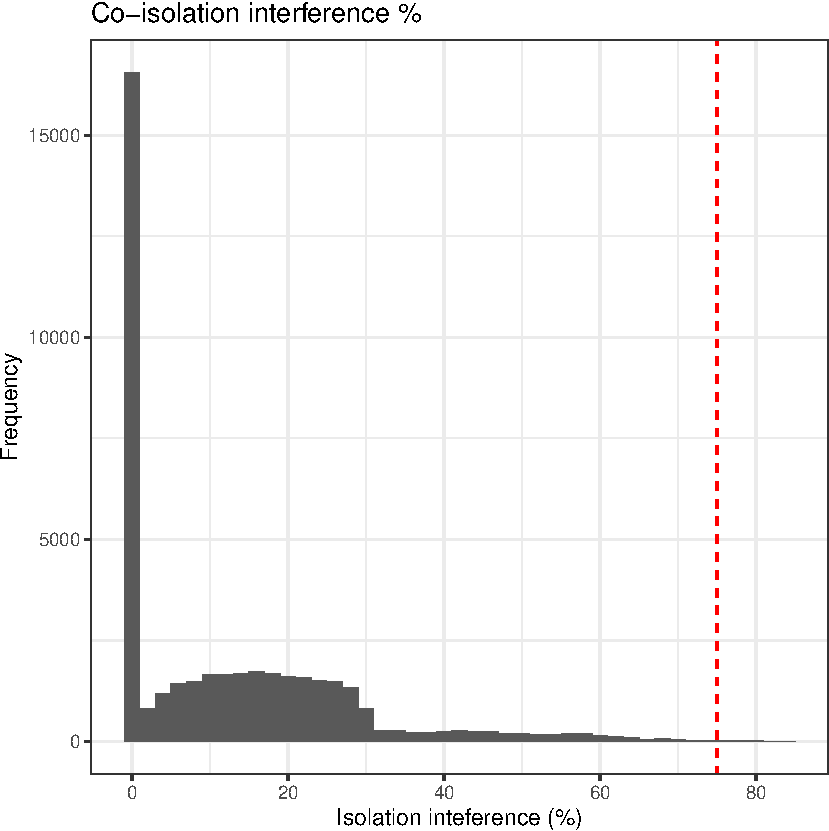
\includegraphics[height=0.3\textheight]{workflow_expressions_files/figure-latex/tmt_coisolation_2-1} \end{center}

Looking at the data, very few PSMs have an isolation interference above the
suggested threshold, and hence minimal data will be lost. Again, we choose to
apply the standard threshold with the understanding that decreasing the
threshold would result in greater data loss. Importantly, we are able to apply
relatively standard thresholds here as the preliminary exploration did not
expose any problems with the experimental data (in terms of labelling or MS
analysis). If users have reason to believe the data is of poorer quality then
more stringent thresholding should be considered.

\begin{Shaded}
\begin{Highlighting}[]
\DocumentationTok{\#\# Find out how many PSMs we expect to lose}
\NormalTok{cp\_qf[[}\StringTok{"psms\_filtered"}\NormalTok{]] }\SpecialCharTok{\%\textgreater{}\%} 
  \FunctionTok{rowData}\NormalTok{() }\SpecialCharTok{\%\textgreater{}\%} 
  \FunctionTok{as\_tibble}\NormalTok{() }\SpecialCharTok{\%\textgreater{}\%} 
\NormalTok{  dplyr}\SpecialCharTok{::}\FunctionTok{count}\NormalTok{(Isolation.Interference.in.Percent }\SpecialCharTok{\textgreater{}} \DecValTok{75}\NormalTok{)}
\end{Highlighting}
\end{Shaded}

\begin{verbatim}
## # A tibble: 2 x 2
##   `Isolation.Interference.in.Percent > 75`     n
##   <lgl>                                    <int>
## 1 FALSE                                    41638
## 2 TRUE                                        58
\end{verbatim}

\begin{Shaded}
\begin{Highlighting}[]
\DocumentationTok{\#\# Remove these rows from the data}
\NormalTok{cp\_qf }\OtherTok{\textless{}{-}}\NormalTok{ cp\_qf }\SpecialCharTok{\%\textgreater{}\%}
  \FunctionTok{filterFeatures}\NormalTok{(}\SpecialCharTok{\textasciitilde{}}\NormalTok{ Isolation.Interference.in.Percent }\SpecialCharTok{\textless{}=} \DecValTok{75}\NormalTok{, }
                 \AttributeTok{na.rm =} \ConstantTok{TRUE}\NormalTok{,}
                 \AttributeTok{i =} \StringTok{"psms\_filtered"}\NormalTok{)}
\end{Highlighting}
\end{Shaded}

\subsubsection{Quality control: SPS mass match}\label{quality-control-sps-mass-match}

The final quality control filter that we will apply is a percentage SPS mass
match threshold. SPS mass match is a metric which has been introduced by
Proteome Discoverer versions 2.3 and above to quantify the percentage of SPS-MS3
fragments that can still be explicitly traced back to the precursor peptide.
This parameter is of particular importance given that quantitation is based on
the SPS-MS3 spectra. Unfortunately, the SPS Mass Match percentage is currently
only a feature of Proteome Discoverer (2.3 and above) and will not be available
to users of other third party software.

We follow the same format as before to investigate the SPS Mass Match (\%)
distribution of the data. The default threshold within Proteome Discoverer is a
SPS Mass Match above 65\%. In reality, since SPS Mass Match is only reported to
the nearest 10\%, removing PSMs annotated with a value below 65\% means removing
those with 60\% or less. Hence, only PSMs with 70\% SPS Mass Match or above would
be retained. We can see how many PSMs would be lost based on such thresholds
using the code chunk below.

\begin{Shaded}
\begin{Highlighting}[]
\DocumentationTok{\#\# Get summary information}
\NormalTok{cp\_qf[[}\StringTok{"psms\_filtered"}\NormalTok{]] }\SpecialCharTok{\%\textgreater{}\%} 
  \FunctionTok{rowData}\NormalTok{() }\SpecialCharTok{\%\textgreater{}\%} 
  \FunctionTok{as\_tibble}\NormalTok{() }\SpecialCharTok{\%\textgreater{}\%} 
  \FunctionTok{pull}\NormalTok{(SPS.Mass.Matches.in.Percent) }\SpecialCharTok{\%\textgreater{}\%} 
  \FunctionTok{summary}\NormalTok{()}
\end{Highlighting}
\end{Shaded}

\begin{verbatim}
##    Min. 1st Qu.  Median    Mean 3rd Qu.    Max. 
##    0.00   50.00   70.00   64.46   80.00  100.00
\end{verbatim}

\begin{Shaded}
\begin{Highlighting}[]
\DocumentationTok{\#\# Plot histogram of SPS mass match \%}
\NormalTok{cp\_qf[[}\StringTok{"psms\_filtered"}\NormalTok{]] }\SpecialCharTok{\%\textgreater{}\%}
  \FunctionTok{rowData}\NormalTok{() }\SpecialCharTok{\%\textgreater{}\%}
  \FunctionTok{as\_tibble}\NormalTok{() }\SpecialCharTok{\%\textgreater{}\%}
  \FunctionTok{ggplot}\NormalTok{(}\FunctionTok{aes}\NormalTok{(}\AttributeTok{x =}\NormalTok{ SPS.Mass.Matches.in.Percent)) }\SpecialCharTok{+}
  \FunctionTok{geom\_histogram}\NormalTok{(}\AttributeTok{binwidth =} \DecValTok{10}\NormalTok{) }\SpecialCharTok{+}
  \FunctionTok{geom\_vline}\NormalTok{(}\AttributeTok{xintercept =} \DecValTok{65}\NormalTok{, }\AttributeTok{linetype =} \StringTok{"dashed"}\NormalTok{, }\AttributeTok{color =} \StringTok{"red"}\NormalTok{) }\SpecialCharTok{+}
  \FunctionTok{labs}\NormalTok{(}\AttributeTok{x =} \StringTok{"SPS mass matches (\%)"}\NormalTok{, }\AttributeTok{y =} \StringTok{"Frequency"}\NormalTok{) }\SpecialCharTok{+}
  \FunctionTok{scale\_x\_continuous}\NormalTok{(}\AttributeTok{breaks =} \FunctionTok{seq}\NormalTok{(}\DecValTok{0}\NormalTok{, }\DecValTok{100}\NormalTok{, }\DecValTok{10}\NormalTok{)) }\SpecialCharTok{+}
  \FunctionTok{ggtitle}\NormalTok{(}\StringTok{"SPS mass match \%"}\NormalTok{) }\SpecialCharTok{+}
  \FunctionTok{theme\_bw}\NormalTok{()}
\end{Highlighting}
\end{Shaded}

\begin{center}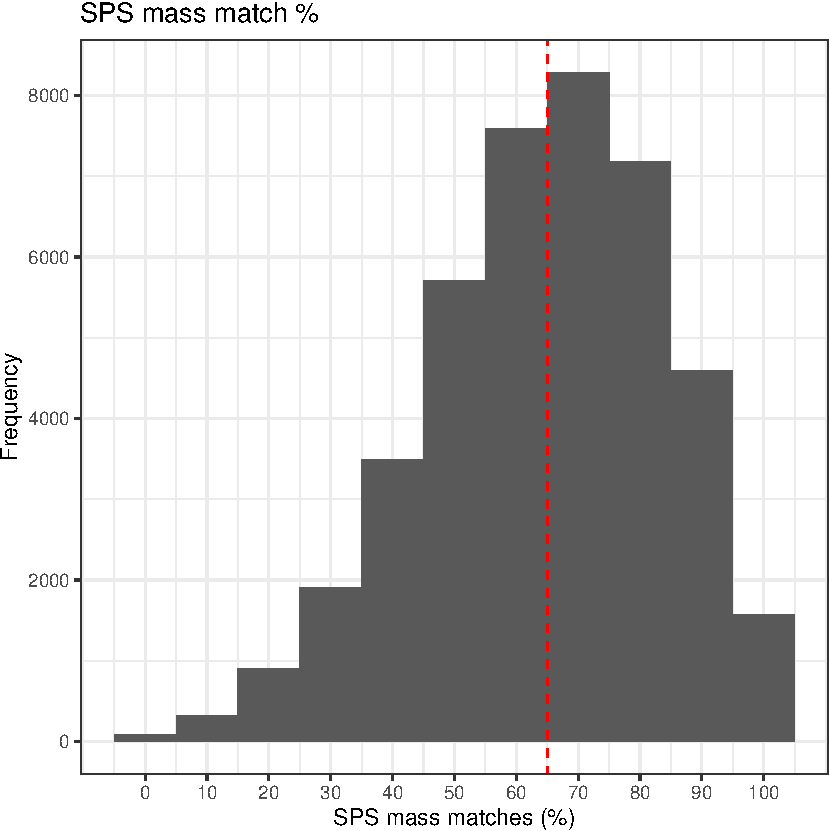
\includegraphics[height=0.3\textheight]{workflow_expressions_files/figure-latex/tmt_sps_matches_2-1} \end{center}

From the summary and histogram we can see that the distribution of SPS Mass
Matches is much less skewed than that of average reporter ion S/N or isolation
interference. This means that whilst the application of thresholds on average
reporter ion S/N and isolation interference led to minimal data loss, attempting
to impose a threshold on SPS Mass Match represents a much greater trade-off
between data quality and quantity. For simplicity, here we choose to use the
standard threshold of 65\%.

\begin{Shaded}
\begin{Highlighting}[]
\DocumentationTok{\#\# Find out how many PSMs we expect to lose}
\NormalTok{cp\_qf[[}\StringTok{"psms\_filtered"}\NormalTok{]] }\SpecialCharTok{\%\textgreater{}\%} 
  \FunctionTok{rowData}\NormalTok{() }\SpecialCharTok{\%\textgreater{}\%} 
  \FunctionTok{as\_tibble}\NormalTok{() }\SpecialCharTok{\%\textgreater{}\%} 
\NormalTok{  dplyr}\SpecialCharTok{::}\FunctionTok{count}\NormalTok{(SPS.Mass.Matches.in.Percent }\SpecialCharTok{\textless{}} \DecValTok{65}\NormalTok{)}
\end{Highlighting}
\end{Shaded}

\begin{verbatim}
## # A tibble: 2 x 2
##   `SPS.Mass.Matches.in.Percent < 65`     n
##   <lgl>                              <int>
## 1 FALSE                              21631
## 2 TRUE                               20007
\end{verbatim}

\begin{Shaded}
\begin{Highlighting}[]
\DocumentationTok{\#\# Drop these rows from the data}
\NormalTok{cp\_qf }\OtherTok{\textless{}{-}}\NormalTok{ cp\_qf }\SpecialCharTok{\%\textgreater{}\%}
  \FunctionTok{filterFeatures}\NormalTok{(}\SpecialCharTok{\textasciitilde{}}\NormalTok{ SPS.Mass.Matches.in.Percent }\SpecialCharTok{\textgreater{}=} \DecValTok{65}\NormalTok{, }
                 \AttributeTok{na.rm =} \ConstantTok{TRUE}\NormalTok{,}
                 \AttributeTok{i =} \StringTok{"psms\_filtered"}\NormalTok{)}
\end{Highlighting}
\end{Shaded}

\subsubsection{Assessing the impact of data-specific filtering}\label{assessing-the-impact-of-data-specific-filtering}

As we did after the non-specific cleaning steps, we check to see how many PSMs,
peptides and proteins have been removed throughout the in-depth data-specific
filtering.

\begin{Shaded}
\begin{Highlighting}[]
\DocumentationTok{\#\# Summarize the effect of data{-}specific filtering}

\DocumentationTok{\#\# Determine the number and proportion of PSMs removed}
\NormalTok{psms\_remaining\_2 }\OtherTok{\textless{}{-}}\NormalTok{ cp\_qf[[}\StringTok{"psms\_filtered"}\NormalTok{]] }\SpecialCharTok{\%\textgreater{}\%}
  \FunctionTok{nrow}\NormalTok{() }\SpecialCharTok{\%\textgreater{}\%}
  \FunctionTok{as.numeric}\NormalTok{()}

\NormalTok{psms\_removed\_2 }\OtherTok{\textless{}{-}}\NormalTok{ psms\_remaining }\SpecialCharTok{{-}}\NormalTok{ psms\_remaining\_2}
\NormalTok{psms\_removed\_prop\_2 }\OtherTok{\textless{}{-}}\NormalTok{ ((psms\_removed\_2 }\SpecialCharTok{/}\NormalTok{ original\_psms) }\SpecialCharTok{*} \DecValTok{100}\NormalTok{) }\SpecialCharTok{\%\textgreater{}\%}
  \FunctionTok{round}\NormalTok{(}\AttributeTok{digits =} \DecValTok{2}\NormalTok{)}


\DocumentationTok{\#\# Determine number and proportion of peptides removed}
\NormalTok{peps\_remaining\_2 }\OtherTok{\textless{}{-}} \FunctionTok{rowData}\NormalTok{(cp\_qf[[}\StringTok{"psms\_filtered"}\NormalTok{]])}\SpecialCharTok{$}\NormalTok{Sequence }\SpecialCharTok{\%\textgreater{}\%}
  \FunctionTok{unique}\NormalTok{() }\SpecialCharTok{\%\textgreater{}\%}
  \FunctionTok{length}\NormalTok{() }\SpecialCharTok{\%\textgreater{}\%}
  \FunctionTok{as.numeric}\NormalTok{()}

\NormalTok{peps\_removed\_2 }\OtherTok{\textless{}{-}}\NormalTok{ peps\_remaining }\SpecialCharTok{{-}}\NormalTok{ peps\_remaining\_2}
\NormalTok{peps\_removed\_prop\_2 }\OtherTok{\textless{}{-}}\NormalTok{ ((peps\_removed\_2 }\SpecialCharTok{/}\NormalTok{ original\_peps) }\SpecialCharTok{*} \DecValTok{100}\NormalTok{) }\SpecialCharTok{\%\textgreater{}\%}
  \FunctionTok{round}\NormalTok{(}\AttributeTok{digits =} \DecValTok{2}\NormalTok{)}


\DocumentationTok{\#\# Determine number and proportion of proteins removed}
\NormalTok{prots\_remaining\_2 }\OtherTok{\textless{}{-}}\NormalTok{ cp\_qf[[}\StringTok{"psms\_filtered"}\NormalTok{]] }\SpecialCharTok{\%\textgreater{}\%}
  \FunctionTok{rowData}\NormalTok{() }\SpecialCharTok{\%\textgreater{}\%}
  \FunctionTok{as\_tibble}\NormalTok{() }\SpecialCharTok{\%\textgreater{}\%}
  \FunctionTok{pull}\NormalTok{(Master.Protein.Accessions) }\SpecialCharTok{\%\textgreater{}\%}
  \FunctionTok{unique}\NormalTok{() }\SpecialCharTok{\%\textgreater{}\%}
  \FunctionTok{length}\NormalTok{() }\SpecialCharTok{\%\textgreater{}\%}
  \FunctionTok{as.numeric}\NormalTok{() }

\NormalTok{prots\_removed\_2 }\OtherTok{\textless{}{-}}\NormalTok{ prots\_remaining }\SpecialCharTok{{-}}\NormalTok{ prots\_remaining\_2}
\NormalTok{prots\_removed\_prop\_2 }\OtherTok{\textless{}{-}}\NormalTok{ ((prots\_removed\_2 }\SpecialCharTok{/}\NormalTok{ original\_prots) }\SpecialCharTok{*} \DecValTok{100}\NormalTok{) }\SpecialCharTok{\%\textgreater{}\%}
  \FunctionTok{round}\NormalTok{(}\AttributeTok{digits =} \DecValTok{2}\NormalTok{)}


\DocumentationTok{\#\# Print as a table}
\FunctionTok{data.frame}\NormalTok{(}\StringTok{"Feature"} \OtherTok{=} \FunctionTok{c}\NormalTok{(}\StringTok{"PSMs"}\NormalTok{,}
                         \StringTok{"Peptides (stripped)"}\NormalTok{,}
                         \StringTok{"Protein groups"}\NormalTok{),}
           \StringTok{"Number lost"} \OtherTok{=} \FunctionTok{c}\NormalTok{(psms\_removed\_2,}
\NormalTok{                             peps\_removed\_2,}
\NormalTok{                             prots\_removed\_2),}
           \StringTok{"Percentage lost"} \OtherTok{=} \FunctionTok{c}\NormalTok{(psms\_removed\_prop\_2,}
\NormalTok{                                 peps\_removed\_prop\_2,}
\NormalTok{                                 prots\_removed\_prop\_2))}
\end{Highlighting}
\end{Shaded}

\begin{verbatim}
##               Feature Number.lost Percentage.lost
## 1                PSMs       21135           43.28
## 2 Peptides (stripped)        9861           37.97
## 3      Protein groups         998           19.80
\end{verbatim}

\subsection{Managing missing data}\label{managing-missing-data}

Having finished the data cleaning at the PSM-level, the final step is to deal
with missing data. Missing values represent a common challenge in quantitative
proteomics and there is no consensus within the literature on how this challenge
should be addressed. Indeed, missing values fall into different categories based
on the reason they were generated, and each category is best dealt with in a
different way. There are three main categories of missing data: missing
completely at random (MCAR), missing at random (MAR) and missing not at random
(MNAR). Within proteomics, values which are MCAR arise due to technical
variation or stochastic fluctuations and emerge in a uniform,
intensity-independent distribution. Examples include values for peptides which
cannot be consistently identified or are unable to be efficiently ionized. By
contrast, MNAR values are expected to occur in an intensity-dependent manner due
to the presence of peptides at abundances below the limit of detection
\citep{Karpievitch2009, Lazar2016, QFeat}. In many cases this is due to the biological
condition being evaluated, for example the cell type or treatment applied.

To simplify this process, we consider the management of missing data in three
steps. The first step is to determine the presence and pattern of missing values
within the data. Next, we filter out data which exceed the desired proportion of
missing values. This includes removing PSMs with a greater number of missing
values across samples than we deem acceptable, as well as whole samples in cases
where the proportion of missing values is substantially higher than the average.
Finally, imputation can be used to replace any remaining NA values within the
dataset. This final step is optional and can equally be done prior to filtering
if the user wishes to impute all missing values without removing any PSMs,
although this is not recommended. Further, whilst it is possible to complete
such steps at the peptide- or protein-level, we advise management of missing
values at the lowest data level to minimize the effect of implicit imputation
during aggregation.

\subsubsection{Exploring the presence of missing values}\label{exploring-the-presence-of-missing-values}

First, to determine the presence of missing values in the PSM-level data we use
the \texttt{nNA} function within the \texttt{QFeatures} infrastructure. This function will
return the absolute number (nNA) and proportion (pNA) of missing values both per
sample and as an average. Importantly, alternative third-party software may
output missing values in formats other than NA, such as zero, or infinite. In
such cases, missing values can be converted directly into NA values through use
of the \texttt{zeroIsNA} or \texttt{infIsNA} functions within the \texttt{QFeatures} infrastructure.

\begin{Shaded}
\begin{Highlighting}[]
\DocumentationTok{\#\# Determine whether there are any NA values in the data}
\NormalTok{cp\_qf[[}\StringTok{"psms\_filtered"}\NormalTok{]] }\SpecialCharTok{\%\textgreater{}\%}
  \FunctionTok{assay}\NormalTok{() }\SpecialCharTok{\%\textgreater{}\%}
  \FunctionTok{anyNA}\NormalTok{()}
\end{Highlighting}
\end{Shaded}

\begin{verbatim}
## [1] TRUE
\end{verbatim}

\begin{Shaded}
\begin{Highlighting}[]
\DocumentationTok{\#\# Determine the amount and distribution of NA values in the data}
\NormalTok{cp\_qf[[}\StringTok{"psms\_filtered"}\NormalTok{]] }\SpecialCharTok{\%\textgreater{}\%}
  \FunctionTok{nNA}\NormalTok{()}
\end{Highlighting}
\end{Shaded}

\begin{verbatim}
## $nNA
## DataFrame with 1 row and 2 columns
##         nNA       pNA
##   <integer> <numeric>
## 1         4 3.082e-05
## 
## $nNArows
## DataFrame with 21631 rows and 3 columns
##              name       nNA       pNA
##       <character> <integer> <numeric>
## 1              13         0         0
## 2              20         0         0
## 3              25         0         0
## 4              26         0         0
## 5              29         0         0
## ...           ...       ...       ...
## 21627       48786         0         0
## 21628       48792         0         0
## 21629       48797         0         0
## 21630       48810         0         0
## 21631       48819         0         0
## 
## $nNAcols
## DataFrame with 6 rows and 3 columns
##          name       nNA         pNA
##   <character> <integer>   <numeric>
## 1          S5         1 4.62299e-05
## 2          S2         2 9.24599e-05
## 3          S1         0 0.00000e+00
## 4          S4         1 4.62299e-05
## 5          S6         0 0.00000e+00
## 6          S3         0 0.00000e+00
\end{verbatim}

We can see that the proportion of missing values in our data is only 3e-05, corresponding to 4 NA values. This low proportion is due to a
combination of the TMT labelling strategy and the stringent PSM quality control
filtering. In particular, co-isolation interference when using TMT labels often
results in very low quantification values for peptides which should actually be
missing or `NA'. Nevertheless, we continue and check for sample-specific bias in
the distribution of NAs by plotting a simple histogram. We will plot percentage
instead of proportion as this is easier to visualise. We also use colour to
indicate the condition of each sample as to check for condition-specific bias.

\begin{Shaded}
\begin{Highlighting}[]
\DocumentationTok{\#\# Plot histogram to visualize the distribution of NAs}
\FunctionTok{nNA}\NormalTok{(cp\_qf[[}\StringTok{"psms\_filtered"}\NormalTok{]])}\SpecialCharTok{$}\NormalTok{nNAcols }\SpecialCharTok{\%\textgreater{}\%}
  \FunctionTok{as\_tibble}\NormalTok{() }\SpecialCharTok{\%\textgreater{}\%}
  \FunctionTok{mutate}\NormalTok{(}\AttributeTok{Condition =} \FunctionTok{c}\NormalTok{(}\StringTok{"Control"}\NormalTok{, }\StringTok{"Treated"}\NormalTok{, }\StringTok{"Treated"}\NormalTok{,}
                       \StringTok{"Control"}\NormalTok{, }\StringTok{"Control"}\NormalTok{, }\StringTok{"Treated"}\NormalTok{)) }\SpecialCharTok{\%\textgreater{}\%}
  \FunctionTok{ggplot}\NormalTok{(}\FunctionTok{aes}\NormalTok{(}\AttributeTok{x =}\NormalTok{ name, }\AttributeTok{y =}\NormalTok{ (pNA }\SpecialCharTok{*} \DecValTok{100}\NormalTok{ ), }\AttributeTok{group =}\NormalTok{ Condition, }\AttributeTok{fill =}\NormalTok{ Condition)) }\SpecialCharTok{+}
  \FunctionTok{geom\_bar}\NormalTok{(}\AttributeTok{stat =} \StringTok{"identity"}\NormalTok{, }\AttributeTok{position =} \StringTok{"dodge"}\NormalTok{) }\SpecialCharTok{+}
  \FunctionTok{labs}\NormalTok{(}\AttributeTok{x =} \StringTok{"Sample"}\NormalTok{, }\AttributeTok{y =} \StringTok{"Missing values (\%)"}\NormalTok{) }\SpecialCharTok{+}
  \FunctionTok{theme\_bw}\NormalTok{()}
\end{Highlighting}
\end{Shaded}

\begin{center}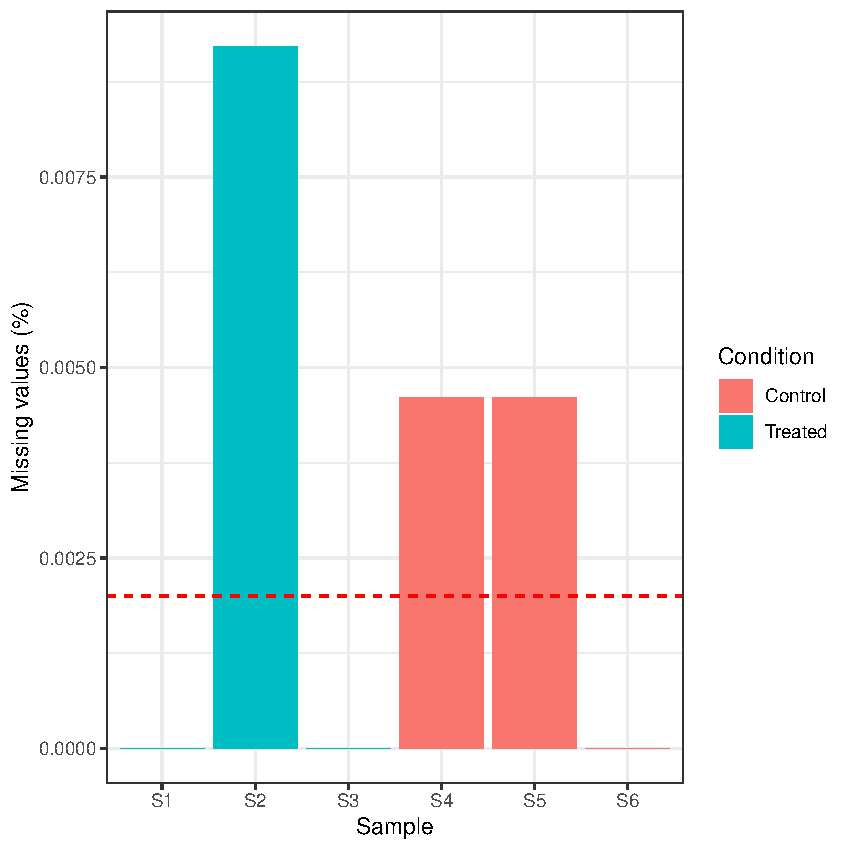
\includegraphics[height=0.4\textheight]{workflow_expressions_files/figure-latex/tmt_missing_data_2-1} \end{center}

The proportion of missing values is sufficiently low that none of the samples
need be removed. Further, there is no sample- or condition-specific bias in the
data. We can get more information about the PSMs with NA values using the code
below.

\begin{Shaded}
\begin{Highlighting}[]
\DocumentationTok{\#\# Find out the range of missing values per PSM}
\FunctionTok{nNA}\NormalTok{(cp\_qf[[}\StringTok{"psms\_filtered"}\NormalTok{]])}\SpecialCharTok{$}\NormalTok{nNArows}\SpecialCharTok{$}\NormalTok{nNA }\SpecialCharTok{\%\textgreater{}\%}
  \FunctionTok{table}\NormalTok{()}
\end{Highlighting}
\end{Shaded}

\begin{verbatim}
## .
##     0     1 
## 21627     4
\end{verbatim}

From this output we can see that the maximum number of NA values per PSM is one.
This information is useful to know as it may inform the filtering strategy in the
next step.

\begin{Shaded}
\begin{Highlighting}[]
\DocumentationTok{\#\# Get indices of rows which contain NA}
\NormalTok{rows\_with\_na\_indices }\OtherTok{\textless{}{-}} \FunctionTok{which}\NormalTok{(}\FunctionTok{nNA}\NormalTok{(cp\_qf[[}\StringTok{"psms\_filtered"}\NormalTok{]])}\SpecialCharTok{$}\NormalTok{nNArows}\SpecialCharTok{$}\NormalTok{nNA }\SpecialCharTok{!=} \DecValTok{0}\NormalTok{)}

\DocumentationTok{\#\# Subset rows with NA}
\NormalTok{rows\_with\_na }\OtherTok{\textless{}{-}}\NormalTok{ cp\_qf[[}\StringTok{"psms\_filtered"}\NormalTok{]][rows\_with\_na\_indices, ]}

\DocumentationTok{\#\# Inspect rows with NA}
\FunctionTok{assay}\NormalTok{(rows\_with\_na)}
\end{Highlighting}
\end{Shaded}

\begin{verbatim}
##         S5   S2   S1   S4   S6   S3
## 12087   NA 17.0 11.0 22.1 30.6 13.3
## 30824 69.7   NA 45.0 66.7 62.1 43.1
## 30846 65.5   NA 34.3 56.8 57.2 47.9
## 44791  3.8 28.7 22.8   NA 12.2 19.6
\end{verbatim}

\subsubsection{Filtering out missing values}\label{filtering-out-missing-values}

First we apply some standard filtering. Typically, it is desirable to remove
features, here PSMs, with greater than 20\% missing values. We can do this using
the \texttt{filterNA} function in \texttt{QFeatures}, as outlined below. We pass the function
the \texttt{SummarizedExperiment} and use the \texttt{pNA\ =} argument to specify the maximum
proportion of NA values to allow.

\begin{Shaded}
\begin{Highlighting}[]
\DocumentationTok{\#\# Check how many PSMs we will remove}
\FunctionTok{nNA}\NormalTok{(cp\_qf[[}\StringTok{"psms\_filtered"}\NormalTok{]])}\SpecialCharTok{$}\NormalTok{nNArows }\SpecialCharTok{\%\textgreater{}\%}
  \FunctionTok{as\_tibble}\NormalTok{() }\SpecialCharTok{\%\textgreater{}\%}
\NormalTok{  dplyr}\SpecialCharTok{::}\FunctionTok{count}\NormalTok{(pNA }\SpecialCharTok{\textgreater{}=} \FloatTok{0.2}\NormalTok{)}
\end{Highlighting}
\end{Shaded}

\begin{verbatim}
## # A tibble: 1 x 2
##   `pNA >= 0.2`     n
##   <lgl>        <int>
## 1 FALSE        21631
\end{verbatim}

Although the use-case data does not contain any PSMs with a higher proportion
of missing values than 0.2, we demonstrate how to apply the desired filter below.

\begin{Shaded}
\begin{Highlighting}[]
\DocumentationTok{\#\# Remove PSMs with more than 20 \% (0.2) NA values}
\NormalTok{cp\_qf }\OtherTok{\textless{}{-}}\NormalTok{ cp\_qf }\SpecialCharTok{\%\textgreater{}\%} 
  \FunctionTok{filterNA}\NormalTok{(}\AttributeTok{pNA =} \FloatTok{0.2}\NormalTok{, }
           \AttributeTok{i =} \StringTok{"psms\_filtered"}\NormalTok{)}
\end{Highlighting}
\end{Shaded}

Since previous exploration of missing data did not reveal any sample with an
excessive number of NA values, we do not need to remove any samples from the
analysis.

Although not covered here, users may wish to carry out condition-specific
filtering in cases where the exploration of missing values revealed a condition-
specific bias, or where the experimental question requires. This would be the
case, for example, if one condition was transfected to express proteins of
interest whilst the control condition lacked these proteins. Filtering of both
conditions together could, therefore, lead to the removal of proteins of interest.

\subsubsection{Imputation (optional)}\label{imputation-optional}

The final step is to consider whether to impute the remaining missing values
within the data. Imputation refers to the replacement of missing values with
probable values. Since imputation requires complex assumptions and can have
substantial effects on downstream statistical analysis, we here choose to skip
imputation. This is reasonable given that we only have 3 missing values at the
PSM-level, and that some of these will likely be removed by aggregation. A more
in-depth discussion of imputation will be provided below in the workflow.

\subsection{Summary of PSM data cleaning}\label{summary-of-psm-data-cleaning}

Thus far we have checked that the experimental data we are using is of high
quality by visualizing the raw data and calculating TMT labelling efficiency. We
then carried out non-specific data cleaning, data-specific filtering steps and
management of missing data. Here, we present a combined summary of these PSM
processing steps.

\begin{Shaded}
\begin{Highlighting}[]
\DocumentationTok{\#\# Determine final number of PSMs, peptides and master proteins}
\NormalTok{psms\_final }\OtherTok{\textless{}{-}}\NormalTok{ cp\_qf[[}\StringTok{"psms\_filtered"}\NormalTok{]] }\SpecialCharTok{\%\textgreater{}\%}
  \FunctionTok{nrow}\NormalTok{() }\SpecialCharTok{\%\textgreater{}\%}
  \FunctionTok{as.numeric}\NormalTok{()}

\NormalTok{psms\_removed\_total }\OtherTok{\textless{}{-}}\NormalTok{ original\_psms }\SpecialCharTok{{-}}\NormalTok{ psms\_final}
\NormalTok{psms\_removed\_total\_prop }\OtherTok{\textless{}{-}}\NormalTok{ ((psms\_removed\_total }\SpecialCharTok{/}\NormalTok{ original\_psms) }\SpecialCharTok{*} \DecValTok{100}\NormalTok{) }\SpecialCharTok{\%\textgreater{}\%}
  \FunctionTok{round}\NormalTok{(}\AttributeTok{digits =} \DecValTok{2}\NormalTok{)}

\NormalTok{peps\_final }\OtherTok{\textless{}{-}}\NormalTok{ cp\_qf[[}\StringTok{"psms\_filtered"}\NormalTok{]] }\SpecialCharTok{\%\textgreater{}\%}
  \FunctionTok{rowData}\NormalTok{() }\SpecialCharTok{\%\textgreater{}\%}
  \FunctionTok{as\_tibble}\NormalTok{() }\SpecialCharTok{\%\textgreater{}\%}
  \FunctionTok{pull}\NormalTok{(Sequence) }\SpecialCharTok{\%\textgreater{}\%}
  \FunctionTok{unique}\NormalTok{() }\SpecialCharTok{\%\textgreater{}\%}
  \FunctionTok{length}\NormalTok{() }\SpecialCharTok{\%\textgreater{}\%}
  \FunctionTok{as.numeric}\NormalTok{()}

\NormalTok{peps\_removed\_total }\OtherTok{\textless{}{-}}\NormalTok{ original\_peps }\SpecialCharTok{{-}}\NormalTok{ peps\_final}
\NormalTok{peps\_removed\_total\_prop }\OtherTok{\textless{}{-}}\NormalTok{ ((peps\_removed\_total }\SpecialCharTok{/}\NormalTok{ original\_peps) }\SpecialCharTok{*} \DecValTok{100}\NormalTok{) }\SpecialCharTok{\%\textgreater{}\%}
  \FunctionTok{round}\NormalTok{(}\AttributeTok{digits =} \DecValTok{2}\NormalTok{)}

\NormalTok{prots\_final }\OtherTok{\textless{}{-}}\NormalTok{ cp\_qf[[}\StringTok{"psms\_filtered"}\NormalTok{]] }\SpecialCharTok{\%\textgreater{}\%}
  \FunctionTok{rowData}\NormalTok{() }\SpecialCharTok{\%\textgreater{}\%}
  \FunctionTok{as\_tibble}\NormalTok{() }\SpecialCharTok{\%\textgreater{}\%}
  \FunctionTok{pull}\NormalTok{(Master.Protein.Accessions) }\SpecialCharTok{\%\textgreater{}\%}
  \FunctionTok{unique}\NormalTok{() }\SpecialCharTok{\%\textgreater{}\%}
  \FunctionTok{length}\NormalTok{() }\SpecialCharTok{\%\textgreater{}\%}
  \FunctionTok{as.numeric}\NormalTok{()}

\NormalTok{prots\_removed\_total }\OtherTok{\textless{}{-}}\NormalTok{ original\_prots }\SpecialCharTok{{-}}\NormalTok{ prots\_final}
\NormalTok{prots\_removed\_total\_prop }\OtherTok{\textless{}{-}}\NormalTok{ ((prots\_removed\_total }\SpecialCharTok{/}\NormalTok{ original\_prots) }\SpecialCharTok{*} \DecValTok{100}\NormalTok{) }\SpecialCharTok{\%\textgreater{}\%}
  \FunctionTok{round}\NormalTok{(}\AttributeTok{digits =} \DecValTok{2}\NormalTok{)}

\DocumentationTok{\#\# Print as table}
\FunctionTok{data.frame}\NormalTok{(}\StringTok{"Feature"} \OtherTok{=} \FunctionTok{c}\NormalTok{(}\StringTok{"PSMs"}\NormalTok{,}
                         \StringTok{"Peptides (stripped)"}\NormalTok{,}
                         \StringTok{"Protein groups"}\NormalTok{),}
           \StringTok{"Number lost"} \OtherTok{=} \FunctionTok{c}\NormalTok{(psms\_removed\_total,}
\NormalTok{                             peps\_removed\_total,}
\NormalTok{                             prots\_removed\_total),}
           \StringTok{"Percentage lost"} \OtherTok{=} \FunctionTok{c}\NormalTok{(psms\_removed\_total\_prop,}
\NormalTok{                                 peps\_removed\_total\_prop,}
\NormalTok{                                 prots\_removed\_total\_prop),}
           \StringTok{"Number remaining"} \OtherTok{=} \FunctionTok{c}\NormalTok{(psms\_final,}
\NormalTok{                                  peps\_final,}
\NormalTok{                                  prots\_final))}
\end{Highlighting}
\end{Shaded}

\begin{verbatim}
##               Feature Number.lost Percentage.lost Number.remaining
## 1                PSMs       27201           55.70            21631
## 2 Peptides (stripped)       11786           45.38            14183
## 3      Protein groups        1810           35.91             3230
\end{verbatim}

\subsection{Logarithmic transformation of quantitative data}\label{logarithmic-transformation-of-quantitative-data}

Once satisfied that the PSM-level data is clean and of high quality, the PSM-level
quantitative data is log transformed. log2 transformation is a standard
step when dealing with quantitative proteomics data since protein abundances are
dramatically skewed towards zero. Such a skewed distribution is to be expected
given that the majority of cellular proteins present at any one time are of
relatively low abundance, whilst only a few highly abundant proteins exist. To
perform the logarithmic transformation and generate normally distributed data we
pass the PSM-level data in the \texttt{QFeatures} object to the \texttt{logTransform}
function, as per the below code chunk.

\begin{Shaded}
\begin{Highlighting}[]
\DocumentationTok{\#\# log2 transform quantitative data}
\NormalTok{cp\_qf }\OtherTok{\textless{}{-}} \FunctionTok{logTransform}\NormalTok{(}\AttributeTok{object =}\NormalTok{ cp\_qf,}
                      \AttributeTok{base =} \DecValTok{2}\NormalTok{,}
                      \AttributeTok{i =} \StringTok{"psms\_filtered"}\NormalTok{,}
                      \AttributeTok{name =} \StringTok{"log\_psms"}\NormalTok{)}

\DocumentationTok{\#\# Verify}
\NormalTok{cp\_qf}
\end{Highlighting}
\end{Shaded}

\begin{verbatim}
## An instance of class QFeatures containing 3 assays:
##  [1] psms_raw: SummarizedExperiment with 48832 rows and 6 columns 
##  [2] psms_filtered: SummarizedExperiment with 21631 rows and 6 columns 
##  [3] log_psms: SummarizedExperiment with 21631 rows and 6 columns
\end{verbatim}

\subsection{Aggregation of PSMs to proteins}\label{aggregation-of-psms-to-proteins}

For the aggregation itself we use the \texttt{aggregateFeatures} function and provide
the base level from which we wish to aggregate, the log PSM-level data in this
case. We also tell the function which column to aggregate which is specified by
the \texttt{fcol} argument. We will first aggregate from PSM to peptide to create
explicit \texttt{QFeatures} links. This means grouping by PSM ``Sequence''.

As well as grouping PSMs according to their peptide sequence, the quantitative
values for each PSM must be aggregated into a single peptide-level value. The
default aggregation method within \texttt{aggregateFeatures} is the \texttt{robustSummary}
function from the
\href{https://bioconductor.org/packages/release/bioc/html/MsCoreUtils.html}{\texttt{MsCoreUtils} package}
\citep{Rainer2022}. This method is a form of robust regression and is described in
detail elsewhere \citep{Sticker2020}. Nevertheless, the user must decide which
aggregation method is most appropriate for their data and biological question.
Further, an understanding of the selected method is critical given that
aggregation is a form of implicit imputation and has substantial effects on the
downstream data. Indeed, aggregation methods have different ways of dealing with
missing data, either by removal or propagation. Options of aggregation methods
within the \texttt{aggregateFeatures} function include
\href{https://rdrr.io/bioc/MsCoreUtils/man/medianPolish.html}{\texttt{MsCoreUtils::medianPolish}},
\href{https://rdrr.io/bioc/MsCoreUtils/man/robustSummary.html}{\texttt{MsCoreUtils::robustSummary}},
\href{https://www.rdocumentation.org/packages/base/versions/3.6.2/topics/colSums}{\texttt{base::colMeans}},
\href{https://www.rdocumentation.org/packages/base/versions/3.6.2/topics/colSums}{\texttt{base::colSums}},
and \href{https://rdrr.io/rforge/matrixStats/man/rowMedians.html}{\texttt{matrixStats::colMedians}}.
Users should also be aware that some methods have specific input requirements.
For example, \texttt{robustSummary} assumes that intensities have already been log
transformed.

\subsubsection{Aggregating using robust summarization}\label{aggregating-using-robust-summarization}

Here, we use \texttt{robustSummary} to aggregate from PSM to peptide-level. This method
is currently considered to be state-of-the-art as it is more robust against
outliers than other aggregation methods \citep{Sticker2020, Goeminne2016}. We also
include \texttt{na.rm\ =\ TRUE} to exclude any NA values prior to completing the
summarization. For simplicity, we here aggregate all PSMs corresponding to the
same stripped peptide sequence, regardless of whether they contain different
modifications. If users are interested in exploring differential expression of
protein isoforms or have reason to believe that post-translational modifications
may be important in answering their question, PSMs could also be aggregated by
\texttt{"Annotated.Sequence"} to preserve this information.

\begin{Shaded}
\begin{Highlighting}[]
\DocumentationTok{\#\# Aggregate PSM to peptide}
\NormalTok{cp\_qf }\OtherTok{\textless{}{-}} \FunctionTok{aggregateFeatures}\NormalTok{(cp\_qf,}
                           \AttributeTok{i =} \StringTok{"log\_psms"}\NormalTok{,}
                           \AttributeTok{fcol =} \StringTok{"Sequence"}\NormalTok{,}
                           \AttributeTok{name =} \StringTok{"log\_peptides"}\NormalTok{,}
                           \AttributeTok{fun =}\NormalTok{ MsCoreUtils}\SpecialCharTok{::}\NormalTok{robustSummary,}
                           \AttributeTok{na.rm =} \ConstantTok{TRUE}\NormalTok{)}
\end{Highlighting}
\end{Shaded}

\begin{verbatim}
## Your quantitative and row data contain missing values. Please read the
## relevant section(s) in the aggregateFeatures manual page regarding the
## effects of missing values on data aggregation.
\end{verbatim}

\begin{Shaded}
\begin{Highlighting}[]
\DocumentationTok{\#\# Verify}
\NormalTok{cp\_qf}
\end{Highlighting}
\end{Shaded}

\begin{verbatim}
## An instance of class QFeatures containing 4 assays:
##  [1] psms_raw: SummarizedExperiment with 48832 rows and 6 columns 
##  [2] psms_filtered: SummarizedExperiment with 21631 rows and 6 columns 
##  [3] log_psms: SummarizedExperiment with 21631 rows and 6 columns 
##  [4] log_peptides: SummarizedExperiment with 14183 rows and 6 columns
\end{verbatim}

We are now left with a \texttt{QFeatures} object holding the PSM and peptide-level data
in their own \texttt{SummarizedExperiment}s. Importantly, an explicit link has been
maintained between the two levels and this makes it possible to gain information
about all PSMs that were aggregated into a peptide.

\subsubsection{Considerations for aggregating non-imputed data}\label{considerations-for-aggregating-non-imputed-data}

If users did not impute prior to aggregation, NA values within the PSM-level
data may have propagated into NaN values. This is because peptides only
supported by PSMs containing missing values would not have any quantitative
value to which a sum or median function, for example, can be applied. Therefore,
we check for NaN and convert back to NA values to facilitate compatibility with
downstream processing.

\begin{Shaded}
\begin{Highlighting}[]
\DocumentationTok{\#\# Confirm the presence of NaN}
\FunctionTok{assay}\NormalTok{(cp\_qf[[}\StringTok{"log\_peptides"}\NormalTok{]]) }\SpecialCharTok{\%\textgreater{}\%}
  \FunctionTok{is.nan}\NormalTok{() }\SpecialCharTok{\%\textgreater{}\%}
  \FunctionTok{table}\NormalTok{()}
\end{Highlighting}
\end{Shaded}

\begin{verbatim}
## .
## FALSE 
## 85098
\end{verbatim}

\begin{Shaded}
\begin{Highlighting}[]
\DocumentationTok{\#\# Replace NaN with NA}
\FunctionTok{assay}\NormalTok{(cp\_qf[[}\StringTok{"log\_peptides"}\NormalTok{]])[}\FunctionTok{is.nan}\NormalTok{(}\FunctionTok{assay}\NormalTok{(cp\_qf[[}\StringTok{"log\_peptides"}\NormalTok{]]))] }\OtherTok{\textless{}{-}} \ConstantTok{NA}
\end{Highlighting}
\end{Shaded}

Next, using the same approach as above, we use the \texttt{aggregateFeatures} function
to assemble the peptides into proteins. As before, we must pass several
arguments to the function. Namely, the \texttt{QFeatures} object i.e.~\texttt{cp\_qf}, the data
level we wish to aggregation from i.e.~\texttt{log\_peptides}, the column of the
\texttt{rowData} defining how to aggregate the features i.e.~by
\texttt{"Master.Protein.Accessions"} and a name for the new data level e.g.
\texttt{"log\_proteins"}. We again choose to use \texttt{robustSummary} as our aggregation
method and we pass \texttt{na.rm\ =\ TRUE} to ignore NA values. Users can type
\texttt{?aggregateFeatures} to see more information. Users should be aware that
peptides are grouped by their master protein accession and, therefore,
downstream differential expression analysis will consider protein groups rather
than individual proteins.

\begin{Shaded}
\begin{Highlighting}[]
\DocumentationTok{\#\# Aggregate peptides to protein}
\NormalTok{cp\_qf }\OtherTok{\textless{}{-}} \FunctionTok{aggregateFeatures}\NormalTok{(cp\_qf,}
                           \AttributeTok{i =} \StringTok{"log\_peptides"}\NormalTok{,}
                           \AttributeTok{fcol =} \StringTok{"Master.Protein.Accessions"}\NormalTok{,}
                           \AttributeTok{name =} \StringTok{"log\_proteins"}\NormalTok{,}
                           \AttributeTok{fun =}\NormalTok{ MsCoreUtils}\SpecialCharTok{::}\NormalTok{robustSummary,}
                           \AttributeTok{na.rm =} \ConstantTok{TRUE}\NormalTok{)}
\end{Highlighting}
\end{Shaded}

\begin{verbatim}
## Your quantitative and row data contain missing values. Please read the
## relevant section(s) in the aggregateFeatures manual page regarding the
## effects of missing values on data aggregation.
\end{verbatim}

\begin{Shaded}
\begin{Highlighting}[]
\DocumentationTok{\#\# Verify}
\NormalTok{cp\_qf}
\end{Highlighting}
\end{Shaded}

\begin{verbatim}
## An instance of class QFeatures containing 5 assays:
##  [1] psms_raw: SummarizedExperiment with 48832 rows and 6 columns 
##  [2] psms_filtered: SummarizedExperiment with 21631 rows and 6 columns 
##  [3] log_psms: SummarizedExperiment with 21631 rows and 6 columns 
##  [4] log_peptides: SummarizedExperiment with 14183 rows and 6 columns 
##  [5] log_proteins: SummarizedExperiment with 3230 rows and 6 columns
\end{verbatim}

Following aggregation, we have a total of 3230
proteins remaining within the data.

\subsection{Normalization of quantitative data}\label{normalization-of-quantitative-data}

After transforming the data, we normalize the protein-level abundances.
Normalization is a process of correction whereby quantitative data is returned
to its original, or `normal', state. In expression proteomics, the aim of post-
acquisition data normalization is to minimize the biases that arises due to
experimental error and technological variation. Specifically, the removal of
random variation and batch effects will allow samples to be aligned prior to
downstream analysis. Importantly, however, users must also be aware of any
normalization that has taken place within their sample preparation, as this will
ultimately influence the presence of differentially abundant proteins
downstream. An extensive review on normalization strategies, both experimental
and computational, is provided in \citep{ORourke2019}.

Unfortunately, there is not currently a single normalization method which
performs best for all quantitative proteomics datasets. That said, the median
(or median-based methods) are a good choice for most quantitative proteomics data.
By contrast, mean normalization is a method to be avoided since the mean is very
sensitive to outliers and we often have such outliers in proteomics data.
Similarly, quantile normalization is not recommended for quantitative proteomics
data due to complications imposed by the presence of missing values. For users
wishing to explore and compare normalization methods, the \href{https://www.bioconductor.org/packages/release/bioc/html/NormalyzerDE.html}{\texttt{NormalyzerDE}},
package within Bioconductor can be used \citep{Willforss2018}.

Here, we will demonstrate the use of a center median normalization approach using
the \texttt{normalize} function within \texttt{QFeatures}.we will apply a center median
approach. To do this, we pass the log transformed protein-level data to the
\texttt{normalize} function in \texttt{QFeatures}. We specify the method of normalization that
we wish to apply i.e.~\texttt{method\ =\ "center.median"} and name the new data level
e.g.~\texttt{name\ =\ "log\_norm\_proteins"}. Of note, for users who wish to apply VSN
normalization the raw protein data must be passed (prior to any log transformation)
as the log transformation is done internally when specify \texttt{method\ =\ "vsn"}. All
other methods require users to explicitly perform log transformation on their
data before use. More details can be found in the \texttt{QFeatures} documentation,
please type \texttt{help("normalize,QFeatures-method")}.

\begin{Shaded}
\begin{Highlighting}[]
\DocumentationTok{\#\# normalize the log transformed peptide data}
\NormalTok{cp\_qf }\OtherTok{\textless{}{-}} \FunctionTok{normalize}\NormalTok{(cp\_qf,}
                   \AttributeTok{i =} \StringTok{"log\_proteins"}\NormalTok{,}
                   \AttributeTok{name =} \StringTok{"log\_norm\_proteins"}\NormalTok{,}
                   \AttributeTok{method =} \StringTok{"center.median"}\NormalTok{)}

\DocumentationTok{\#\# Verify}
\NormalTok{cp\_qf}
\end{Highlighting}
\end{Shaded}

\begin{verbatim}
## An instance of class QFeatures containing 6 assays:
##  [1] psms_raw: SummarizedExperiment with 48832 rows and 6 columns 
##  [2] psms_filtered: SummarizedExperiment with 21631 rows and 6 columns 
##  [3] log_psms: SummarizedExperiment with 21631 rows and 6 columns 
##  [4] log_peptides: SummarizedExperiment with 14183 rows and 6 columns 
##  [5] log_proteins: SummarizedExperiment with 3230 rows and 6 columns 
##  [6] log_norm_proteins: SummarizedExperiment with 3230 rows and 6 columns
\end{verbatim}

To evaluate the effect of normalization we plot a simple boxplot.

\begin{Shaded}
\begin{Highlighting}[]
\DocumentationTok{\#\# Evaluate the effect of data normalization}
\NormalTok{pre\_norm }\OtherTok{\textless{}{-}}\NormalTok{ cp\_qf[[}\StringTok{"log\_proteins"}\NormalTok{]] }\SpecialCharTok{\%\textgreater{}\%}
  \FunctionTok{assay}\NormalTok{() }\SpecialCharTok{\%\textgreater{}\%}
  \FunctionTok{longFormat}\NormalTok{() }\SpecialCharTok{\%\textgreater{}\%}
  \FunctionTok{mutate}\NormalTok{(}\AttributeTok{Condition =} \FunctionTok{ifelse}\NormalTok{(colname }\SpecialCharTok{\%in\%} \FunctionTok{c}\NormalTok{(}\StringTok{"S1"}\NormalTok{, }\StringTok{"S2"}\NormalTok{, }\StringTok{"S3"}\NormalTok{),}
                            \StringTok{"Treated"}\NormalTok{, }\StringTok{"Control"}\NormalTok{),}
         \AttributeTok{colname =} \FunctionTok{factor}\NormalTok{(colname, }\AttributeTok{levels =} \FunctionTok{paste0}\NormalTok{(}\StringTok{"S"}\NormalTok{, }\DecValTok{1}\SpecialCharTok{:}\DecValTok{6}\NormalTok{))) }\SpecialCharTok{\%\textgreater{}\%}
  \FunctionTok{ggplot}\NormalTok{(}\FunctionTok{aes}\NormalTok{(}\AttributeTok{x =}\NormalTok{ colname, }\AttributeTok{y =}\NormalTok{ value, }\AttributeTok{fill =}\NormalTok{ Condition)) }\SpecialCharTok{+}
  \FunctionTok{geom\_boxplot}\NormalTok{() }\SpecialCharTok{+}
  \FunctionTok{labs}\NormalTok{(}\AttributeTok{x =} \StringTok{"Sample"}\NormalTok{, }\AttributeTok{y =} \StringTok{"log2(abundance)"}\NormalTok{, }\AttributeTok{title =} \StringTok{"Pre{-}normalization"}\NormalTok{) }\SpecialCharTok{+}
  \FunctionTok{theme\_bw}\NormalTok{()}

\NormalTok{post\_norm }\OtherTok{\textless{}{-}}\NormalTok{ cp\_qf[[}\StringTok{"log\_norm\_proteins"}\NormalTok{]] }\SpecialCharTok{\%\textgreater{}\%}
  \FunctionTok{assay}\NormalTok{() }\SpecialCharTok{\%\textgreater{}\%}
  \FunctionTok{longFormat}\NormalTok{() }\SpecialCharTok{\%\textgreater{}\%}
  \FunctionTok{mutate}\NormalTok{(}\AttributeTok{Condition =} \FunctionTok{ifelse}\NormalTok{(colname }\SpecialCharTok{\%in\%} \FunctionTok{c}\NormalTok{(}\StringTok{"S1"}\NormalTok{, }\StringTok{"S2"}\NormalTok{, }\StringTok{"S3"}\NormalTok{),}
                            \StringTok{"Treated"}\NormalTok{, }\StringTok{"Control"}\NormalTok{),}
         \AttributeTok{colname =} \FunctionTok{factor}\NormalTok{(colname, }\AttributeTok{levels =} \FunctionTok{paste0}\NormalTok{(}\StringTok{"S"}\NormalTok{, }\DecValTok{1}\SpecialCharTok{:}\DecValTok{6}\NormalTok{))) }\SpecialCharTok{\%\textgreater{}\%}
  \FunctionTok{ggplot}\NormalTok{(}\FunctionTok{aes}\NormalTok{(}\AttributeTok{x =}\NormalTok{ colname, }\AttributeTok{y =}\NormalTok{ value, }\AttributeTok{fill =}\NormalTok{ Condition)) }\SpecialCharTok{+}
  \FunctionTok{geom\_boxplot}\NormalTok{() }\SpecialCharTok{+}
  \FunctionTok{labs}\NormalTok{(}\AttributeTok{x =} \StringTok{"Sample"}\NormalTok{, }\AttributeTok{y =} \StringTok{"log2(abundance)"}\NormalTok{, }\AttributeTok{title =} \StringTok{"Post{-}normalization"}\NormalTok{) }\SpecialCharTok{+}
  \FunctionTok{theme\_bw}\NormalTok{()}

\NormalTok{(pre\_norm }\SpecialCharTok{+} \FunctionTok{theme}\NormalTok{(}\AttributeTok{legend.position =} \StringTok{"none"}\NormalTok{)) }\SpecialCharTok{+} 
\NormalTok{  post\_norm }\SpecialCharTok{\&} \FunctionTok{plot\_layout}\NormalTok{(}\AttributeTok{guides =} \StringTok{"collect"}\NormalTok{)}
\end{Highlighting}
\end{Shaded}

\begin{center}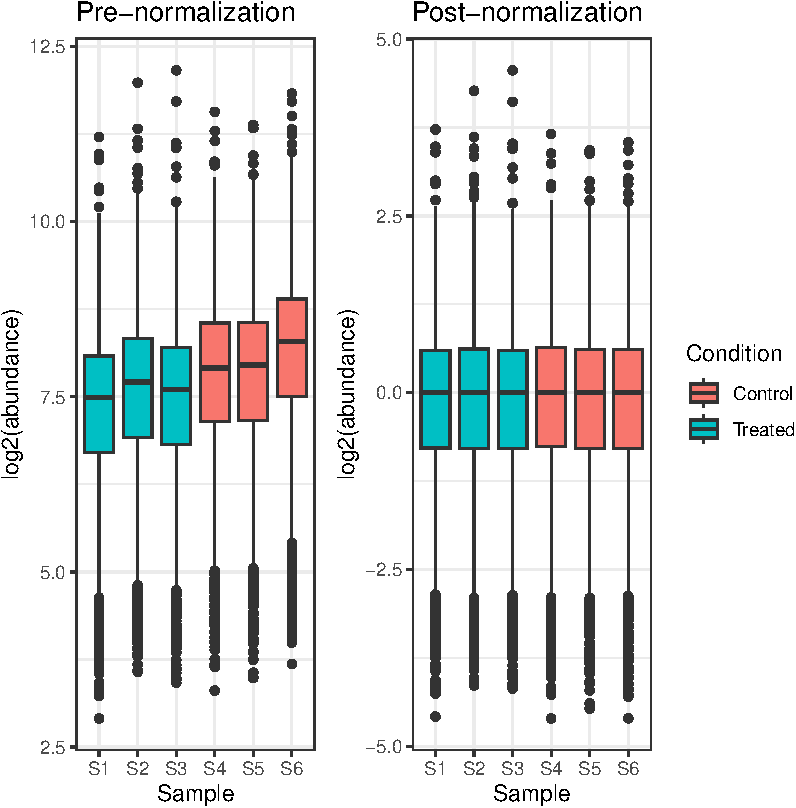
\includegraphics[height=0.4\textheight]{workflow_expressions_files/figure-latex/tmt_normalization_2-1} \end{center}

We can now generate a density plot to help us visualize what the process of log
transformation and normalization has done to the data. This is done using the
\texttt{plotDensities} function from the \texttt{limma} package.

\begin{Shaded}
\begin{Highlighting}[]
\DocumentationTok{\#\# visualize the process of log transformation and normalization}
\FunctionTok{par}\NormalTok{(}\AttributeTok{mfrow =} \FunctionTok{c}\NormalTok{(}\DecValTok{1}\NormalTok{, }\DecValTok{3}\NormalTok{))}

\NormalTok{cp\_qf[[}\StringTok{"psms\_filtered"}\NormalTok{]] }\SpecialCharTok{\%\textgreater{}\%}
  \FunctionTok{assay}\NormalTok{() }\SpecialCharTok{\%\textgreater{}\%}
  \FunctionTok{plotDensities}\NormalTok{(}\AttributeTok{legend =} \StringTok{"topright"}\NormalTok{,}
                \AttributeTok{main =} \StringTok{"Raw PSMs"}\NormalTok{)}

\NormalTok{cp\_qf[[}\StringTok{"log\_psms"}\NormalTok{]] }\SpecialCharTok{\%\textgreater{}\%}
  \FunctionTok{assay}\NormalTok{() }\SpecialCharTok{\%\textgreater{}\%}
  \FunctionTok{plotDensities}\NormalTok{(}\AttributeTok{legend =} \ConstantTok{FALSE}\NormalTok{,}
                \AttributeTok{main =} \StringTok{"log2(PSMs)"}\NormalTok{)}

\NormalTok{cp\_qf[[}\StringTok{"log\_norm\_proteins"}\NormalTok{]] }\SpecialCharTok{\%\textgreater{}\%}
  \FunctionTok{assay}\NormalTok{() }\SpecialCharTok{\%\textgreater{}\%}
  \FunctionTok{plotDensities}\NormalTok{(}\AttributeTok{legend =} \ConstantTok{FALSE}\NormalTok{,}
                \AttributeTok{main =} \StringTok{"log2(norm proteins)"}\NormalTok{)}
\end{Highlighting}
\end{Shaded}

\begin{center}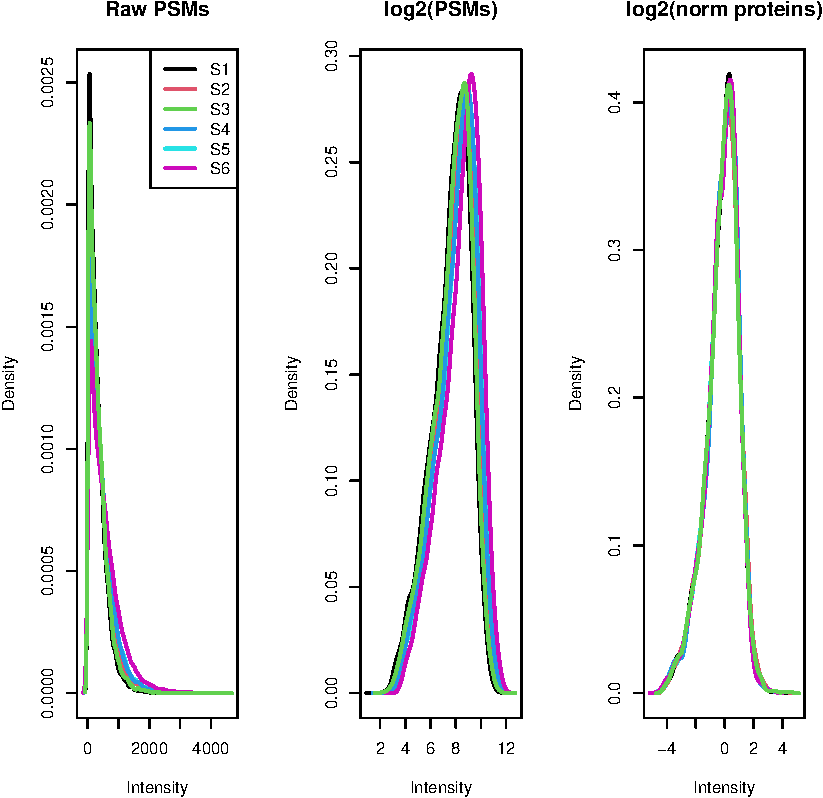
\includegraphics[width=0.9\linewidth]{workflow_expressions_files/figure-latex/tmt_transformations-1} \end{center}

Density plots are a useful vizualization tool as we are able to quickly compare
the data across samples by plotting the distribution of each sample together.
When doing this we get an idea of where the majority of the intensities lie. If,
for example, all samples come from the same cells and our treatment/conditions
don't cause massive changes to the proteome, we expect the distributions of the
intensities to be roughly the same. Above, we see that the raw data before
normalization (left), log2 normalized (middle) and post normalization (right).
In the first two plots the curves/peaks are at different locations but after
normalization (right) we see that we have shifted the curves according to their
median and all peaks of samples are now overlapping.

\subsection{Exploration of data using QFeatures links}\label{exploration-of-data-using-qfeatures-links}

\subsection{Creating assay links}\label{creating-assay-links}

After completing all data pre-processing, we now add explicit links between our
final protein-level data and the raw PSM-level data which we created as an
untouched copy. This allows us to investigate all data corresponding to the
final proteins, including the data that has since been removed. To do this, we
use the \texttt{addAssayLinks} function, demonstrated below. We can check that the
assay links have been generated correctly by passing our \texttt{QFeatures} object to
the \texttt{AssayLink} function along with the assay of interest (\texttt{i\ =}).

\begin{Shaded}
\begin{Highlighting}[]
\DocumentationTok{\#\# Add assay links from log\_norm\_proteins to psms\_raw}
\NormalTok{cp\_qf }\OtherTok{\textless{}{-}} \FunctionTok{addAssayLink}\NormalTok{(}\AttributeTok{object =}\NormalTok{ cp\_qf, }
                      \AttributeTok{from =} \StringTok{"psms\_raw"}\NormalTok{,}
                      \AttributeTok{to =} \StringTok{"log\_norm\_proteins"}\NormalTok{,}
                      \AttributeTok{varFrom =} \StringTok{"Master.Protein.Accessions"}\NormalTok{,}
                      \AttributeTok{varTo =} \StringTok{"Master.Protein.Accessions"}\NormalTok{)}

\DocumentationTok{\#\# Verify}
\FunctionTok{assayLink}\NormalTok{(cp\_qf, }
          \AttributeTok{i =} \StringTok{"log\_norm\_proteins"}\NormalTok{)}
\end{Highlighting}
\end{Shaded}

\begin{verbatim}
## AssayLink for assay <log_norm_proteins>
## [from:psms_raw|fcol:Master.Protein.Accessions|hits:42604]
\end{verbatim}

\subsubsection{visualizing aggregation}\label{visualizing-aggregation}

One of the characteristic attributes of the \texttt{QFeatures} infrastructure is that
explicit links have been maintained throughout the aggregation process. This
means that we can now access all data corresponding to a protein, its component
peptides and PSMs. One way to do this is through the use of the
\texttt{subsetByFeature} function which will return a new \texttt{QFeatures} object containing
data for the desired feature across all levels. For example, if we wish to
subset information about the protein ``Q01581'', that is hydroxymethylglutaryl-CoA
synthase, we could use the following code:

\begin{Shaded}
\begin{Highlighting}[]
\DocumentationTok{\#\# Subset all data linked to the protein with accession Q01581}
\NormalTok{Q01581 }\OtherTok{\textless{}{-}} \FunctionTok{subsetByFeature}\NormalTok{(cp\_qf, }\StringTok{"Q01581"}\NormalTok{)}

\DocumentationTok{\#\# Verify}
\NormalTok{Q01581}
\end{Highlighting}
\end{Shaded}

\begin{verbatim}
## An instance of class QFeatures containing 6 assays:
##  [1] psms_raw: SummarizedExperiment with 42 rows and 6 columns 
##  [2] psms_filtered: SummarizedExperiment with 27 rows and 6 columns 
##  [3] log_psms: SummarizedExperiment with 27 rows and 6 columns 
##  [4] log_peptides: SummarizedExperiment with 15 rows and 6 columns 
##  [5] log_proteins: SummarizedExperiment with 1 rows and 6 columns 
##  [6] log_norm_proteins: SummarizedExperiment with 1 rows and 6 columns
\end{verbatim}

We find that in this data the protein Q01581 has 15
peptides and 27 PSMs supporting its identification
and quantitation. We also see that the original data prior to processing contained
42 PSMs in support of this protein.

Further, we can visualize the process of aggregation that has led to the protein-
level abundance data for Q01581, as demonstrated below. Of note, this plot shows
the protein data prior to transformation.

\begin{Shaded}
\begin{Highlighting}[]
\DocumentationTok{\#\# Define conditions}
\NormalTok{treament }\OtherTok{\textless{}{-}} \FunctionTok{c}\NormalTok{(}\StringTok{"S1"}\NormalTok{, }\StringTok{"S2"}\NormalTok{, }\StringTok{"S3"}\NormalTok{)}
\NormalTok{control }\OtherTok{\textless{}{-}} \FunctionTok{c}\NormalTok{(}\StringTok{"S4"}\NormalTok{, }\StringTok{"S5"}\NormalTok{, }\StringTok{"S6"}\NormalTok{)}

\DocumentationTok{\#\# Plot abundance distributions across samples at PSM, peptide and protein{-}level}
\NormalTok{Q01581[, , }\FunctionTok{c}\NormalTok{(}\StringTok{"log\_psms"}\NormalTok{, }\StringTok{"log\_peptides"}\NormalTok{, }\StringTok{"log\_proteins"}\NormalTok{)] }\SpecialCharTok{\%\textgreater{}\%}
  \FunctionTok{longFormat}\NormalTok{() }\SpecialCharTok{\%\textgreater{}\%}
  \FunctionTok{as\_tibble}\NormalTok{() }\SpecialCharTok{\%\textgreater{}\%}
  \FunctionTok{mutate}\NormalTok{(}\AttributeTok{assay\_order =} \FunctionTok{factor}\NormalTok{(}
\NormalTok{    assay,}
    \AttributeTok{levels =} \FunctionTok{c}\NormalTok{(}\StringTok{"log\_psms"}\NormalTok{, }\StringTok{"log\_peptides"}\NormalTok{, }\StringTok{"log\_proteins"}\NormalTok{),}
    \AttributeTok{labels =} \FunctionTok{c}\NormalTok{(}\StringTok{"PSMs"}\NormalTok{, }\StringTok{"Peptides"}\NormalTok{, }\StringTok{"Protein"}\NormalTok{)),}
    \AttributeTok{condition =} \FunctionTok{ifelse}\NormalTok{(colname }\SpecialCharTok{\%in\%}\NormalTok{ control, }\StringTok{"control"}\NormalTok{, }\StringTok{"treatment"}\NormalTok{)) }\SpecialCharTok{\%\textgreater{}\%}
  \FunctionTok{ggplot}\NormalTok{(}\FunctionTok{aes}\NormalTok{(}\AttributeTok{x =}\NormalTok{ colname, }\AttributeTok{y =}\NormalTok{ value, }\AttributeTok{colour =}\NormalTok{ assay)) }\SpecialCharTok{+}
  \FunctionTok{geom\_point}\NormalTok{(}\AttributeTok{size =} \DecValTok{3}\NormalTok{) }\SpecialCharTok{+}
  \FunctionTok{geom\_line}\NormalTok{(}\FunctionTok{aes}\NormalTok{(}\AttributeTok{group =}\NormalTok{ rowname)) }\SpecialCharTok{+}
  \FunctionTok{scale\_x\_discrete}\NormalTok{(}\AttributeTok{limits =} \FunctionTok{paste0}\NormalTok{(}\StringTok{"S"}\NormalTok{, }\DecValTok{1}\SpecialCharTok{:}\DecValTok{6}\NormalTok{)) }\SpecialCharTok{+}
  \FunctionTok{facet\_wrap}\NormalTok{(}\SpecialCharTok{\textasciitilde{}}\NormalTok{assay\_order) }\SpecialCharTok{+}
  \FunctionTok{labs}\NormalTok{(}\AttributeTok{x =} \StringTok{"Sample"}\NormalTok{, }\AttributeTok{y =} \StringTok{"Abundance"}\NormalTok{) }\SpecialCharTok{+}
  \FunctionTok{ggtitle}\NormalTok{(}\StringTok{"log2 Q01581 abundance profiles"}\NormalTok{) }\SpecialCharTok{+}
  \FunctionTok{theme\_bw}\NormalTok{()}
\end{Highlighting}
\end{Shaded}

\begin{center}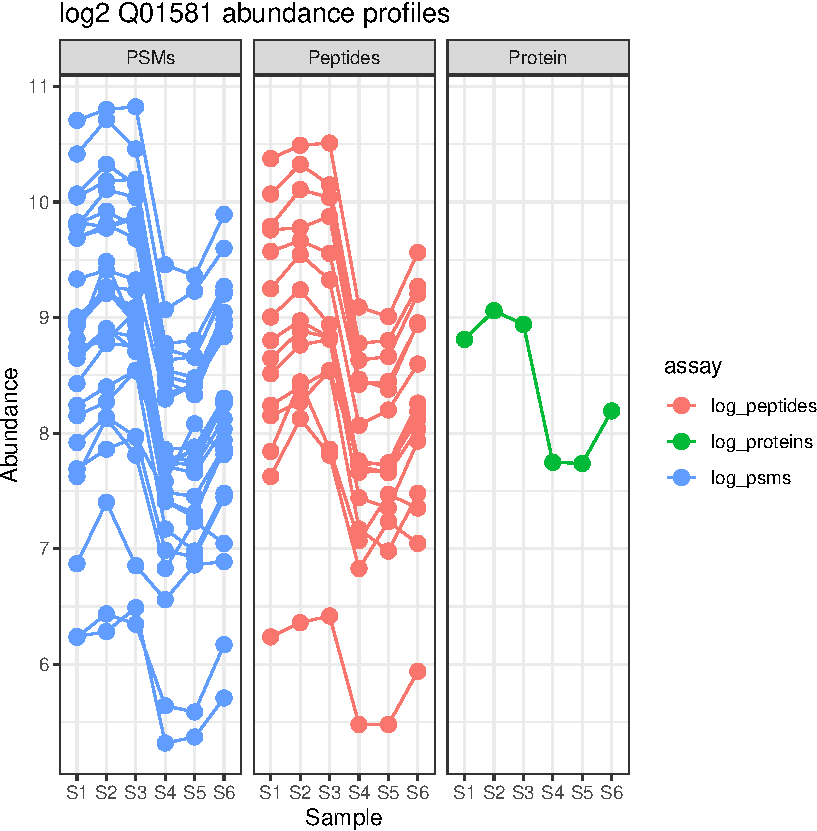
\includegraphics[width=0.8\linewidth]{workflow_expressions_files/figure-latex/qfeatures_links_plots-1} \end{center}

\subsubsection{Determining PSM and peptide support}\label{determining-psm-and-peptide-support}

Another benefit of the explicit links maintained within a \texttt{QFeatures} object is
the ease at which we can determine PSM and peptide support per protein. When
applying the \texttt{aggregateFeatures} function a column, termed \texttt{".n"}, is created
within the rowData of the new \texttt{SummarizedExperiment}. This column indicates how
many lower-level features were aggregated into each new higher-level feature.
Hence, \texttt{".n"} in the peptide-level data represents how many PSMs were aggregated
into a peptide, whilst in the protein-level data it tells us how many peptides
were grouped into a master protein. As an example, we plot the a histogram of
\texttt{".n"} from the protein-level to explore peptide support per protein.

\begin{Shaded}
\begin{Highlighting}[]
\DocumentationTok{\#\# Plot peptide support per protein {-} .n in the proteins SE}
\NormalTok{cp\_qf[[}\StringTok{"log\_proteins"}\NormalTok{]] }\SpecialCharTok{\%\textgreater{}\%}
  \FunctionTok{rowData}\NormalTok{() }\SpecialCharTok{\%\textgreater{}\%}
  \FunctionTok{as\_tibble}\NormalTok{() }\SpecialCharTok{\%\textgreater{}\%}
  \FunctionTok{ggplot}\NormalTok{(}\FunctionTok{aes}\NormalTok{(}\AttributeTok{x =}\NormalTok{ .n)) }\SpecialCharTok{+}
  \FunctionTok{geom\_histogram}\NormalTok{(}\AttributeTok{binwidth =} \DecValTok{1}\NormalTok{, }\AttributeTok{boundary =} \FloatTok{0.5}\NormalTok{) }\SpecialCharTok{+}
  \FunctionTok{labs}\NormalTok{(}\AttributeTok{x =} \StringTok{"Peptide support (shown up to 20)"}\NormalTok{,}
       \AttributeTok{y =} \StringTok{"Frequency"}\NormalTok{) }\SpecialCharTok{+}
  \FunctionTok{scale\_x\_continuous}\NormalTok{(}\AttributeTok{expand =} \FunctionTok{c}\NormalTok{(}\DecValTok{0}\NormalTok{, }\DecValTok{0}\NormalTok{),}
                     \AttributeTok{limits =} \FunctionTok{c}\NormalTok{(}\DecValTok{0}\NormalTok{, }\FloatTok{20.5}\NormalTok{),}
                     \AttributeTok{breaks =} \FunctionTok{seq}\NormalTok{(}\DecValTok{1}\NormalTok{, }\DecValTok{20}\NormalTok{, }\DecValTok{1}\NormalTok{)) }\SpecialCharTok{+}
  \FunctionTok{scale\_y\_continuous}\NormalTok{(}\AttributeTok{expand =} \FunctionTok{c}\NormalTok{(}\DecValTok{0}\NormalTok{, }\DecValTok{0}\NormalTok{),}
                     \AttributeTok{limits =} \FunctionTok{c}\NormalTok{(}\DecValTok{0}\NormalTok{, }\DecValTok{1100}\NormalTok{),}
                     \AttributeTok{breaks =} \FunctionTok{seq}\NormalTok{(}\DecValTok{0}\NormalTok{, }\DecValTok{1100}\NormalTok{, }\DecValTok{100}\NormalTok{)) }\SpecialCharTok{+}
  \FunctionTok{ggtitle}\NormalTok{(}\StringTok{"Peptide support per protein"}\NormalTok{) }\SpecialCharTok{+}
  \FunctionTok{theme\_bw}\NormalTok{()}
\end{Highlighting}
\end{Shaded}

\begin{center}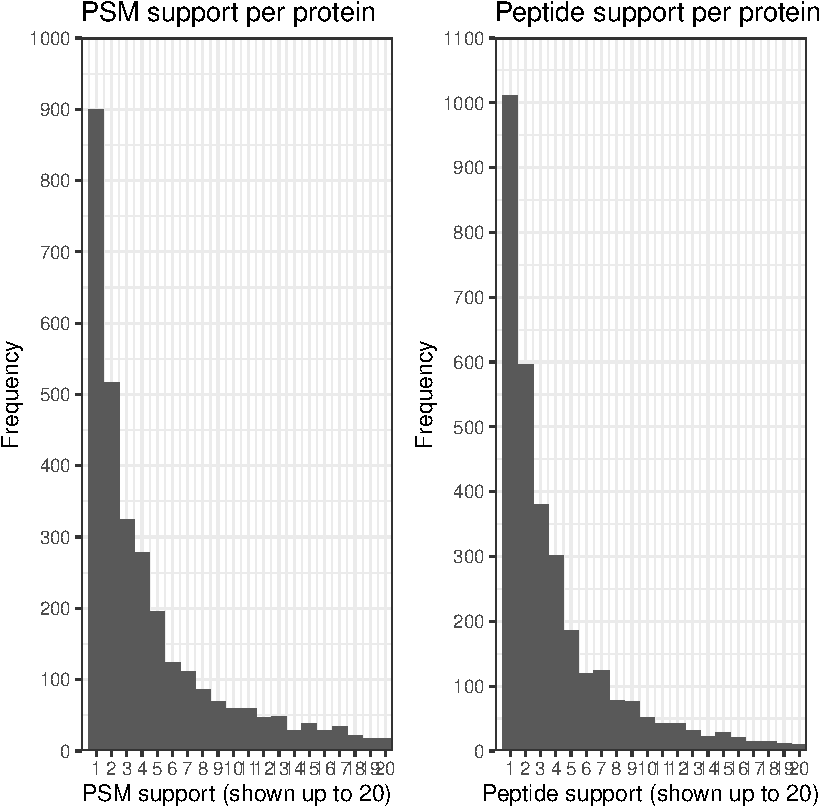
\includegraphics[width=1\linewidth]{workflow_expressions_files/figure-latex/support_plots-1} \end{center}

At this point, users may wish to include additional quality control filtering
based on PSM and/or peptide support per protein. Given the extensive quality
control filtering already applied in this workflow, we decide not to remove
additional proteins based on PSM or peptide support.

\subsection{Data export}\label{data-export}

Finally, we save the protein-level data and export the \texttt{QFeatures} object into
an \texttt{.rda} file so that we can re-load it later at convenience.

\begin{Shaded}
\begin{Highlighting}[]
\DocumentationTok{\#\# Save protein{-}level SE}
\NormalTok{cp\_proteins }\OtherTok{\textless{}{-}}\NormalTok{ cp\_qf[[}\StringTok{"log\_norm\_proteins"}\NormalTok{]]}

\DocumentationTok{\#\# Export the final TMT QFeatures object}
\FunctionTok{save}\NormalTok{(cp\_qf, }\AttributeTok{file =} \StringTok{"cp\_qf.rda"}\NormalTok{)}
\end{Highlighting}
\end{Shaded}

\section{Label-free data processing workflow}\label{label-free-data-processing-workflow}

Having discussed the processing of quantitative TMT-labelled data, we now move
on to consider that of label-free quantitative (LFQ) data. As described
previously, the cell culture supernatant fractions of triplicate control and
treated HEK293 cells were kept label-free. As such, each sample was analyzed using
an independent mass spectrometry run without pre-fractionation. Again, a two-hour
gradient in an Orbitrap Lumos Tribrid mass spectrometer coupled to an UltiMate
3000 HPLC system was applied. Given that much of the TMT pre-processing workflow
also applies to label-free data, we only discuss steps which are different to
those previously described. Readers are advised to refer to the TMT processing
workflow for a more in-depth explanation of any shared steps.

\subsection{Identification search using Proteome Discoverer}\label{identification-search-using-proteome-discoverer}

As was the case for TMT labelled cell pellets, raw LFQ data from supernatant
samples was searched using Proteome Discoverer 2.5. The workflows for this
identification search are provided in the supplementary materials with an additional
explanation of key parameters in the appendix. To begin processing LFQ data,
users should export a peptide-level \texttt{.txt} file from the results of their
identification search.

\subsection{Data import, housekeeping and exploration}\label{data-import-housekeeping-and-exploration-1}

Unlike the TMT-labelled use-case data which was processed from the PSM-level, the
label-free use-case data can only be considered from the peptide-level up. This
is because a retention time alignment algorithm (equivalent to match between runs)
was applied to the PSM-level data. This means that peptides can be identified in
samples even without a corresponding PSM, simply by sharing feature information
across runs.

\subsubsection{Importing data into a QFeatures object}\label{importing-data-into-a-qfeatures-object}

We locate the PeptideGroups \texttt{.txt} file and upload this into a \texttt{data.frame}
container in the same way as before. Since the samples are already stored in the
correct order, we simply identify the quantitative columns by their indices.

\begin{Shaded}
\begin{Highlighting}[]
\DocumentationTok{\#\# Locate the PeptideGroups .txt file}
\NormalTok{sn\_peptide }\OtherTok{\textless{}{-}} \StringTok{"supernatant\_lfq\_results\_peptides.txt"}

\DocumentationTok{\#\# Import into a data.frame}
\NormalTok{sn\_df }\OtherTok{\textless{}{-}} \FunctionTok{read.delim}\NormalTok{(sn\_peptide)}

\DocumentationTok{\#\# Identify columns containing quantitative data}
\NormalTok{sn\_df }\SpecialCharTok{\%\textgreater{}\%}
  \FunctionTok{names}\NormalTok{()}
\end{Highlighting}
\end{Shaded}

\begin{verbatim}
##  [1] "Peptide.Groups.Peptide.Group.ID"                
##  [2] "Checked"                                        
##  [3] "Tags"                                           
##  [4] "Confidence"                                     
##  [5] "PSM.Ambiguity"                                  
##  [6] "Sequence"                                       
##  [7] "Modifications"                                  
##  [8] "Modifications.all.possible.sites"               
##  [9] "Qvality.PEP"                                    
## [10] "Qvality.q.value"                                
## [11] "SVM_Score"                                      
## [12] "Number.of.Protein.Groups"                       
## [13] "Number.of.Proteins"                             
## [14] "Number.of.PSMs"                                 
## [15] "Master.Protein.Accessions"                      
## [16] "Master.Protein.Descriptions"                    
## [17] "Protein.Accessions"                             
## [18] "Number.of.Missed.Cleavages"                     
## [19] "Theo.MHplus.in.Da"                              
## [20] "Sequence.Length"                                
## [21] "Abundance.F1.Sample"                            
## [22] "Abundance.F2.Sample"                            
## [23] "Abundance.F3.Sample"                            
## [24] "Abundance.F4.Sample"                            
## [25] "Abundance.F5.Sample"                            
## [26] "Abundance.F6.Sample"                            
## [27] "Abundances.Count.F1.Sample"                     
## [28] "Abundances.Count.F2.Sample"                     
## [29] "Abundances.Count.F3.Sample"                     
## [30] "Abundances.Count.F4.Sample"                     
## [31] "Abundances.Count.F5.Sample"                     
## [32] "Abundances.Count.F6.Sample"                     
## [33] "Quan.Info"                                      
## [34] "Found.in.File.in.F1"                            
## [35] "Found.in.File.in.F2"                            
## [36] "Found.in.File.in.F3"                            
## [37] "Found.in.File.in.F4"                            
## [38] "Found.in.File.in.F5"                            
## [39] "Found.in.File.in.F6"                            
## [40] "Found.in.Sample.in.S1.F1.Sample"                
## [41] "Found.in.Sample.in.S2.F2.Sample"                
## [42] "Found.in.Sample.in.S3.F3.Sample"                
## [43] "Found.in.Sample.in.S4.F4.Sample"                
## [44] "Found.in.Sample.in.S5.F5.Sample"                
## [45] "Found.in.Sample.in.S6.F6.Sample"                
## [46] "Found.in.Sample.Group.in.S1.F1.Sample"          
## [47] "Found.in.Sample.Group.in.S2.F2.Sample"          
## [48] "Found.in.Sample.Group.in.S3.F3.Sample"          
## [49] "Found.in.Sample.Group.in.S4.F4.Sample"          
## [50] "Found.in.Sample.Group.in.S5.F5.Sample"          
## [51] "Found.in.Sample.Group.in.S6.F6.Sample"          
## [52] "Confidence.by.Search.Engine.Sequest.HT"         
## [53] "Charge.by.Search.Engine.Sequest.HT"             
## [54] "Delta.Score.by.Search.Engine.Sequest.HT"        
## [55] "Delta.Cn.by.Search.Engine.Sequest.HT"           
## [56] "Rank.by.Search.Engine.Sequest.HT"               
## [57] "Search.Engine.Rank.by.Search.Engine.Sequest.HT" 
## [58] "Concatenated.Rank.by.Search.Engine.Sequest.HT"  
## [59] "mz.in.Da.by.Search.Engine.Sequest.HT"           
## [60] "Delta.M.in.ppm.by.Search.Engine.Sequest.HT"     
## [61] "Delta.mz.in.Da.by.Search.Engine.Sequest.HT"     
## [62] "RT.in.min.by.Search.Engine.Sequest.HT"          
## [63] "Percolator.q.Value.by.Search.Engine.Sequest.HT" 
## [64] "Percolator.PEP.by.Search.Engine.Sequest.HT"     
## [65] "Percolator.SVMScore.by.Search.Engine.Sequest.HT"
## [66] "XCorr.by.Search.Engine.Sequest.HT"              
## [67] "Top.Apex.RT.in.min"
\end{verbatim}

In the code chunk below, we again use the \texttt{readQFeatures} function to create a
\texttt{QFeatures} object. We find the abundance data is located in columns 21 to 26
and thus pass this to \texttt{quantCols}. After import we annotate the \texttt{colData}.

\begin{Shaded}
\begin{Highlighting}[]
\DocumentationTok{\#\# Create QFeatures object }
\NormalTok{sn\_qf }\OtherTok{\textless{}{-}} \FunctionTok{readQFeatures}\NormalTok{(}\AttributeTok{assayData =}\NormalTok{ sn\_df,}
                       \AttributeTok{quantCols =} \DecValTok{21}\SpecialCharTok{:}\DecValTok{26}\NormalTok{,}
                       \AttributeTok{name =} \StringTok{"peptides\_raw"}\NormalTok{)}
\end{Highlighting}
\end{Shaded}

\begin{verbatim}
## Checking arguments.
\end{verbatim}

\begin{verbatim}
## Loading data as a 'SummarizedExperiment' object.
\end{verbatim}

\begin{verbatim}
## Formatting sample annotations (colData).
\end{verbatim}

\begin{verbatim}
## Formatting data as a 'QFeatures' object.
\end{verbatim}

\begin{Shaded}
\begin{Highlighting}[]
\DocumentationTok{\#\# Clean sample names}
\FunctionTok{colnames}\NormalTok{(sn\_qf[[}\StringTok{"peptides\_raw"}\NormalTok{]]) }\OtherTok{\textless{}{-}} \FunctionTok{paste0}\NormalTok{(}\StringTok{"S"}\NormalTok{, }\DecValTok{1}\SpecialCharTok{:}\DecValTok{6}\NormalTok{)}

\DocumentationTok{\#\# Annotate samples}
\NormalTok{sn\_qf}\SpecialCharTok{$}\NormalTok{sample }\OtherTok{\textless{}{-}} \FunctionTok{paste0}\NormalTok{(}\StringTok{"S"}\NormalTok{, }\DecValTok{1}\SpecialCharTok{:}\DecValTok{6}\NormalTok{)}

\NormalTok{sn\_qf}\SpecialCharTok{$}\NormalTok{condition }\OtherTok{\textless{}{-}} \FunctionTok{rep}\NormalTok{(}\FunctionTok{c}\NormalTok{(}\StringTok{"Treated"}\NormalTok{, }\StringTok{"Control"}\NormalTok{), }\AttributeTok{each =} \DecValTok{3}\NormalTok{)}

\DocumentationTok{\#\# Verify and allocate colData to initial SummarizedExperiment}
\FunctionTok{colData}\NormalTok{(sn\_qf)}
\end{Highlighting}
\end{Shaded}

\begin{verbatim}
## DataFrame with 6 rows and 2 columns
##         sample   condition
##    <character> <character>
## S1          S1     Treated
## S2          S2     Treated
## S3          S3     Treated
## S4          S4     Control
## S5          S5     Control
## S6          S6     Control
\end{verbatim}

\begin{Shaded}
\begin{Highlighting}[]
\FunctionTok{colData}\NormalTok{(sn\_qf[[}\StringTok{"peptides\_raw"}\NormalTok{]]) }\OtherTok{\textless{}{-}} \FunctionTok{colData}\NormalTok{(sn\_qf)}
\end{Highlighting}
\end{Shaded}

\subsubsection{Preliminary data exploration}\label{preliminary-data-exploration-1}

Next, we check the names of the features within the peptide-level \texttt{rowData}.
These features differ from those found at the PSM-level and users should be
aware that they have reduced post-search control over the quality of PSMs
included in the peptide quantitation, and which method of aggregation is used to
define these. Proteome Discoverer uses the sum of PSM quantitative values to
calculate peptide-level values. Other third-party software may use different
methods.

\begin{Shaded}
\begin{Highlighting}[]
\DocumentationTok{\#\# Find out what information was imported}
\NormalTok{sn\_qf[[}\StringTok{"peptides\_raw"}\NormalTok{]] }\SpecialCharTok{\%\textgreater{}\%}
  \FunctionTok{rowData}\NormalTok{() }\SpecialCharTok{\%\textgreater{}\%}
  \FunctionTok{colnames}\NormalTok{()}
\end{Highlighting}
\end{Shaded}

\begin{verbatim}
##  [1] "Peptide.Groups.Peptide.Group.ID"                
##  [2] "Checked"                                        
##  [3] "Tags"                                           
##  [4] "Confidence"                                     
##  [5] "PSM.Ambiguity"                                  
##  [6] "Sequence"                                       
##  [7] "Modifications"                                  
##  [8] "Modifications.all.possible.sites"               
##  [9] "Qvality.PEP"                                    
## [10] "Qvality.q.value"                                
## [11] "SVM_Score"                                      
## [12] "Number.of.Protein.Groups"                       
## [13] "Number.of.Proteins"                             
## [14] "Number.of.PSMs"                                 
## [15] "Master.Protein.Accessions"                      
## [16] "Master.Protein.Descriptions"                    
## [17] "Protein.Accessions"                             
## [18] "Number.of.Missed.Cleavages"                     
## [19] "Theo.MHplus.in.Da"                              
## [20] "Sequence.Length"                                
## [21] "Abundances.Count.F1.Sample"                     
## [22] "Abundances.Count.F2.Sample"                     
## [23] "Abundances.Count.F3.Sample"                     
## [24] "Abundances.Count.F4.Sample"                     
## [25] "Abundances.Count.F5.Sample"                     
## [26] "Abundances.Count.F6.Sample"                     
## [27] "Quan.Info"                                      
## [28] "Found.in.File.in.F1"                            
## [29] "Found.in.File.in.F2"                            
## [30] "Found.in.File.in.F3"                            
## [31] "Found.in.File.in.F4"                            
## [32] "Found.in.File.in.F5"                            
## [33] "Found.in.File.in.F6"                            
## [34] "Found.in.Sample.in.S1.F1.Sample"                
## [35] "Found.in.Sample.in.S2.F2.Sample"                
## [36] "Found.in.Sample.in.S3.F3.Sample"                
## [37] "Found.in.Sample.in.S4.F4.Sample"                
## [38] "Found.in.Sample.in.S5.F5.Sample"                
## [39] "Found.in.Sample.in.S6.F6.Sample"                
## [40] "Found.in.Sample.Group.in.S1.F1.Sample"          
## [41] "Found.in.Sample.Group.in.S2.F2.Sample"          
## [42] "Found.in.Sample.Group.in.S3.F3.Sample"          
## [43] "Found.in.Sample.Group.in.S4.F4.Sample"          
## [44] "Found.in.Sample.Group.in.S5.F5.Sample"          
## [45] "Found.in.Sample.Group.in.S6.F6.Sample"          
## [46] "Confidence.by.Search.Engine.Sequest.HT"         
## [47] "Charge.by.Search.Engine.Sequest.HT"             
## [48] "Delta.Score.by.Search.Engine.Sequest.HT"        
## [49] "Delta.Cn.by.Search.Engine.Sequest.HT"           
## [50] "Rank.by.Search.Engine.Sequest.HT"               
## [51] "Search.Engine.Rank.by.Search.Engine.Sequest.HT" 
## [52] "Concatenated.Rank.by.Search.Engine.Sequest.HT"  
## [53] "mz.in.Da.by.Search.Engine.Sequest.HT"           
## [54] "Delta.M.in.ppm.by.Search.Engine.Sequest.HT"     
## [55] "Delta.mz.in.Da.by.Search.Engine.Sequest.HT"     
## [56] "RT.in.min.by.Search.Engine.Sequest.HT"          
## [57] "Percolator.q.Value.by.Search.Engine.Sequest.HT" 
## [58] "Percolator.PEP.by.Search.Engine.Sequest.HT"     
## [59] "Percolator.SVMScore.by.Search.Engine.Sequest.HT"
## [60] "XCorr.by.Search.Engine.Sequest.HT"              
## [61] "Top.Apex.RT.in.min"
\end{verbatim}

We also determine the number of PSMs, peptides and proteins represented within
the initial data. Since identical peptide sequences with different modifications
are stored as separate entities, the output of \texttt{dim} will not tell us the number
of peptides. Instead, we need to consider only unique peptide sequence entries,
as demonstrated in the code chunk below.

\begin{Shaded}
\begin{Highlighting}[]
\DocumentationTok{\#\# Determine the number of PSMs}
\NormalTok{original\_psms }\OtherTok{\textless{}{-}}\NormalTok{ sn\_qf[[}\StringTok{"peptides\_raw"}\NormalTok{]] }\SpecialCharTok{\%\textgreater{}\%} 
  \FunctionTok{rowData}\NormalTok{() }\SpecialCharTok{\%\textgreater{}\%} 
  \FunctionTok{as\_tibble}\NormalTok{() }\SpecialCharTok{\%\textgreater{}\%} 
  \FunctionTok{pull}\NormalTok{(Number.of.PSMs) }\SpecialCharTok{\%\textgreater{}\%} 
  \FunctionTok{sum}\NormalTok{() }

\DocumentationTok{\#\# Determine the number of peptides}
\NormalTok{original\_peps }\OtherTok{\textless{}{-}}\NormalTok{ sn\_qf[[}\StringTok{"peptides\_raw"}\NormalTok{]] }\SpecialCharTok{\%\textgreater{}\%} 
  \FunctionTok{rowData}\NormalTok{() }\SpecialCharTok{\%\textgreater{}\%} 
  \FunctionTok{as\_tibble}\NormalTok{() }\SpecialCharTok{\%\textgreater{}\%} 
  \FunctionTok{pull}\NormalTok{(Sequence) }\SpecialCharTok{\%\textgreater{}\%} 
  \FunctionTok{unique}\NormalTok{() }\SpecialCharTok{\%\textgreater{}\%}
  \FunctionTok{length}\NormalTok{() }\SpecialCharTok{\%\textgreater{}\%}
  \FunctionTok{as.numeric}\NormalTok{() }

\DocumentationTok{\#\# Determine the number of proteins}
\NormalTok{original\_prots }\OtherTok{\textless{}{-}}\NormalTok{ sn\_qf[[}\StringTok{"peptides\_raw"}\NormalTok{]] }\SpecialCharTok{\%\textgreater{}\%}
  \FunctionTok{rowData}\NormalTok{() }\SpecialCharTok{\%\textgreater{}\%} 
  \FunctionTok{as\_tibble}\NormalTok{() }\SpecialCharTok{\%\textgreater{}\%} 
  \FunctionTok{pull}\NormalTok{(Master.Protein.Accessions) }\SpecialCharTok{\%\textgreater{}\%} 
  \FunctionTok{unique}\NormalTok{() }\SpecialCharTok{\%\textgreater{}\%} 
  \FunctionTok{length}\NormalTok{() }\SpecialCharTok{\%\textgreater{}\%}
  \FunctionTok{as.numeric}\NormalTok{()}

\DocumentationTok{\#\# View}
\NormalTok{original\_psms}
\end{Highlighting}
\end{Shaded}

\begin{verbatim}
## [1] 144302
\end{verbatim}

\begin{Shaded}
\begin{Highlighting}[]
\NormalTok{original\_peps}
\end{Highlighting}
\end{Shaded}

\begin{verbatim}
## [1] 20312
\end{verbatim}

\begin{Shaded}
\begin{Highlighting}[]
\NormalTok{original\_prots}
\end{Highlighting}
\end{Shaded}

\begin{verbatim}
## [1] 3941
\end{verbatim}

Thus, the search identified 144302 PSMs
corresponding to 20312 peptides and
3941 proteins. Finally, we take a look at some of the key
parameters applied during the identification search. This is an important
verification step, particularly for those using publicly available data with
limited access to parameter settings.

\begin{Shaded}
\begin{Highlighting}[]
\DocumentationTok{\#\# Check missed cleavages}
\NormalTok{sn\_qf[[}\StringTok{"peptides\_raw"}\NormalTok{]] }\SpecialCharTok{\%\textgreater{}\%}
  \FunctionTok{rowData}\NormalTok{() }\SpecialCharTok{\%\textgreater{}\%} 
  \FunctionTok{as\_tibble}\NormalTok{() }\SpecialCharTok{\%\textgreater{}\%} 
  \FunctionTok{pull}\NormalTok{(Number.of.Missed.Cleavages) }\SpecialCharTok{\%\textgreater{}\%} 
  \FunctionTok{table}\NormalTok{()}
\end{Highlighting}
\end{Shaded}

\begin{verbatim}
## .
##     0     1     2 
## 22055  1248    72
\end{verbatim}

\begin{Shaded}
\begin{Highlighting}[]
\DocumentationTok{\#\# Check precursor mass tolerance}
\NormalTok{sn\_qf[[}\StringTok{"peptides\_raw"}\NormalTok{]] }\SpecialCharTok{\%\textgreater{}\%}
  \FunctionTok{rowData}\NormalTok{() }\SpecialCharTok{\%\textgreater{}\%} 
  \FunctionTok{as\_tibble}\NormalTok{() }\SpecialCharTok{\%\textgreater{}\%} 
  \FunctionTok{pull}\NormalTok{(Delta.M.in.ppm.by.Search.Engine.Sequest.HT) }\SpecialCharTok{\%\textgreater{}\%} 
  \FunctionTok{summary}\NormalTok{()}
\end{Highlighting}
\end{Shaded}

\begin{verbatim}
##    Min. 1st Qu.  Median    Mean 3rd Qu.    Max. 
## -9.9600 -0.2500  0.1500  0.6576  0.6900  9.9900
\end{verbatim}

\begin{Shaded}
\begin{Highlighting}[]
\DocumentationTok{\#\# Check fragment mass tolerance}
\NormalTok{sn\_qf[[}\StringTok{"peptides\_raw"}\NormalTok{]] }\SpecialCharTok{\%\textgreater{}\%}
  \FunctionTok{rowData}\NormalTok{() }\SpecialCharTok{\%\textgreater{}\%} 
  \FunctionTok{as\_tibble}\NormalTok{() }\SpecialCharTok{\%\textgreater{}\%} 
  \FunctionTok{pull}\NormalTok{(Delta.mz.in.Da.by.Search.Engine.Sequest.HT) }\SpecialCharTok{\%\textgreater{}\%} 
  \FunctionTok{summary}\NormalTok{()}
\end{Highlighting}
\end{Shaded}

\begin{verbatim}
##       Min.    1st Qu.     Median       Mean    3rd Qu.       Max. 
## -0.0113400 -0.0001400  0.0000900  0.0006618  0.0004800  0.0142300
\end{verbatim}

\begin{Shaded}
\begin{Highlighting}[]
\DocumentationTok{\#\# Check peptide confidence allocations}
\NormalTok{sn\_qf[[}\StringTok{"peptides\_raw"}\NormalTok{]] }\SpecialCharTok{\%\textgreater{}\%}
  \FunctionTok{rowData}\NormalTok{() }\SpecialCharTok{\%\textgreater{}\%} 
  \FunctionTok{as\_tibble}\NormalTok{() }\SpecialCharTok{\%\textgreater{}\%} 
  \FunctionTok{pull}\NormalTok{(Confidence) }\SpecialCharTok{\%\textgreater{}\%} 
  \FunctionTok{table}\NormalTok{()}
\end{Highlighting}
\end{Shaded}

\begin{verbatim}
## .
##  High 
## 23375
\end{verbatim}

The preliminary data is as expected so we continue on to evaluate the quality
of the raw data.

\subsection{Experimental quality control checks}\label{experimental-quality-control-checks-1}

\subsubsection{Quality control of the raw mass spectrometry data}\label{quality-control-of-the-raw-mass-spectrometry-data-1}

To briefly assess the quality of the raw mass spectrometry data from which the
search results were derived, we create simple plots. In contrast to the previous
PSM processing workflow, we do not have access to information about ion injection
times from the peptide-level file. However, we can still look at the peptide
delta mass across retention time, as well as the frequency of peptides across
the retention time gradient.

\begin{Shaded}
\begin{Highlighting}[]
\DocumentationTok{\#\# Plot scatter plot of mass accuracy}
\NormalTok{sn\_qf[[}\StringTok{"peptides\_raw"}\NormalTok{]] }\SpecialCharTok{\%\textgreater{}\%}
  \FunctionTok{rowData}\NormalTok{() }\SpecialCharTok{\%\textgreater{}\%}
  \FunctionTok{as\_tibble}\NormalTok{() }\SpecialCharTok{\%\textgreater{}\%}
  \FunctionTok{ggplot}\NormalTok{(}\FunctionTok{aes}\NormalTok{(}\AttributeTok{x =}\NormalTok{ RT.in.min.by.Search.Engine.Sequest.HT,}
             \AttributeTok{y =}\NormalTok{ Delta.M.in.ppm.by.Search.Engine.Sequest.HT)) }\SpecialCharTok{+}
  \FunctionTok{geom\_point}\NormalTok{(}\AttributeTok{size =} \FloatTok{0.5}\NormalTok{, }\AttributeTok{shape =} \DecValTok{4}\NormalTok{) }\SpecialCharTok{+}
  \FunctionTok{geom\_hline}\NormalTok{(}\AttributeTok{yintercept =} \DecValTok{5}\NormalTok{, }\AttributeTok{linetype =} \StringTok{"dashed"}\NormalTok{, }\AttributeTok{color =} \StringTok{"red"}\NormalTok{) }\SpecialCharTok{+}
  \FunctionTok{geom\_hline}\NormalTok{(}\AttributeTok{yintercept =} \SpecialCharTok{{-}}\DecValTok{5}\NormalTok{, }\AttributeTok{linetype =} \StringTok{"dashed"}\NormalTok{, }\AttributeTok{color =} \StringTok{"red"}\NormalTok{) }\SpecialCharTok{+}
  \FunctionTok{labs}\NormalTok{(}\AttributeTok{x =} \StringTok{"RT (min)"}\NormalTok{, }\AttributeTok{y =} \StringTok{"Delta precursor mass (ppm)"}\NormalTok{) }\SpecialCharTok{+}
  \FunctionTok{scale\_x\_continuous}\NormalTok{(}\AttributeTok{limits =} \FunctionTok{c}\NormalTok{(}\DecValTok{0}\NormalTok{, }\DecValTok{120}\NormalTok{), }\AttributeTok{breaks =} \FunctionTok{seq}\NormalTok{(}\DecValTok{0}\NormalTok{, }\DecValTok{120}\NormalTok{, }\DecValTok{20}\NormalTok{)) }\SpecialCharTok{+}
  \FunctionTok{scale\_y\_continuous}\NormalTok{(}\AttributeTok{limits =} \FunctionTok{c}\NormalTok{(}\SpecialCharTok{{-}}\DecValTok{10}\NormalTok{, }\DecValTok{10}\NormalTok{), }\AttributeTok{breaks =} \FunctionTok{c}\NormalTok{(}\SpecialCharTok{{-}}\DecValTok{10}\NormalTok{, }\SpecialCharTok{{-}}\DecValTok{5}\NormalTok{, }\DecValTok{0}\NormalTok{, }\DecValTok{5}\NormalTok{, }\DecValTok{10}\NormalTok{)) }\SpecialCharTok{+}
  \FunctionTok{ggtitle}\NormalTok{(}\StringTok{"Peptide retention time against delta precursor mass"}\NormalTok{) }\SpecialCharTok{+}
  \FunctionTok{theme\_bw}\NormalTok{()}
\end{Highlighting}
\end{Shaded}

\begin{center}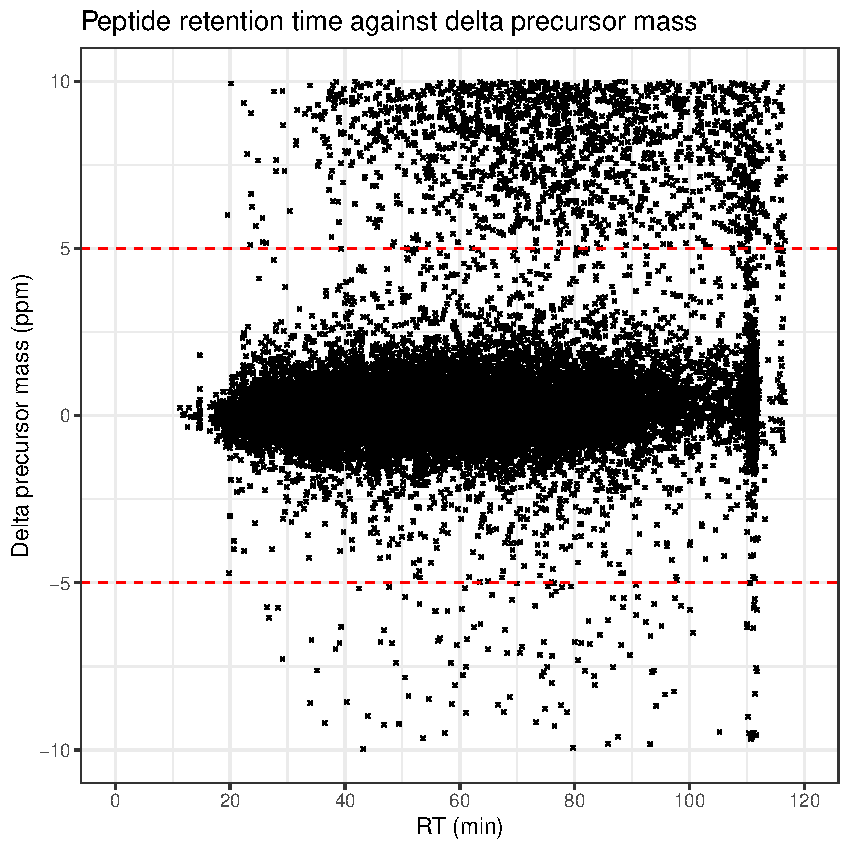
\includegraphics[height=0.3\textheight]{workflow_expressions_files/figure-latex/lfq_mass_accuracy-1} \end{center}

\begin{Shaded}
\begin{Highlighting}[]
\DocumentationTok{\#\# Plot histogram of peptide retention time}
\NormalTok{sn\_qf[[}\StringTok{"peptides\_raw"}\NormalTok{]] }\SpecialCharTok{\%\textgreater{}\%}
  \FunctionTok{rowData}\NormalTok{() }\SpecialCharTok{\%\textgreater{}\%}
  \FunctionTok{as\_tibble}\NormalTok{() }\SpecialCharTok{\%\textgreater{}\%}
  \FunctionTok{ggplot}\NormalTok{(}\FunctionTok{aes}\NormalTok{(}\AttributeTok{x =}\NormalTok{ RT.in.min.by.Search.Engine.Sequest.HT)) }\SpecialCharTok{+}
  \FunctionTok{geom\_histogram}\NormalTok{(}\AttributeTok{binwidth =} \DecValTok{1}\NormalTok{) }\SpecialCharTok{+}
  \FunctionTok{labs}\NormalTok{(}\AttributeTok{x =} \StringTok{"RT (min)"}\NormalTok{, }\AttributeTok{y =} \StringTok{"Frequency"}\NormalTok{) }\SpecialCharTok{+}
  \FunctionTok{scale\_x\_continuous}\NormalTok{(}\AttributeTok{breaks =} \FunctionTok{seq}\NormalTok{(}\DecValTok{0}\NormalTok{, }\DecValTok{120}\NormalTok{, }\DecValTok{20}\NormalTok{)) }\SpecialCharTok{+}
  \FunctionTok{ggtitle}\NormalTok{(}\StringTok{"Peptide frequency across retention time"}\NormalTok{) }\SpecialCharTok{+}
  \FunctionTok{theme\_bw}\NormalTok{()}
\end{Highlighting}
\end{Shaded}

\begin{center}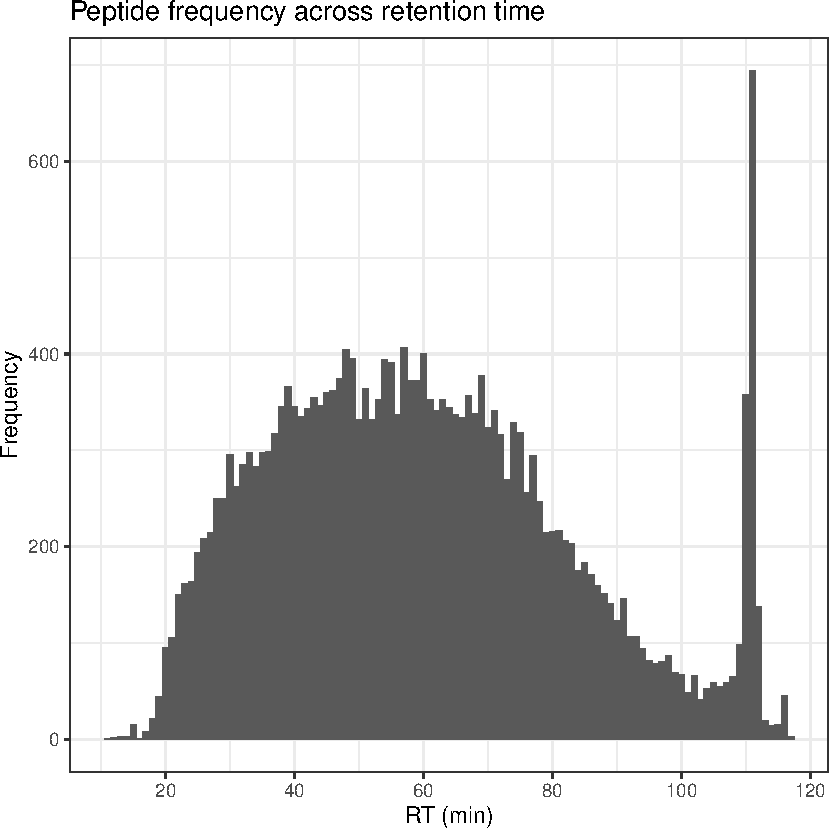
\includegraphics[height=0.3\textheight]{workflow_expressions_files/figure-latex/lfq_RT-1} \end{center}

For a more in-depth discussion of these plots users should refer back to the TMT
processing workflow. Since neither plot indicates any major problems with the MS
runs, we continue on to basic data cleaning.

\subsection{Basic data cleaning}\label{basic-data-cleaning-1}

As discussed in detail above, there are several basic data cleaning steps which
are non-specific and should be applied to all quantitative datasets, regardless
of the quantitation method or data level (PSM, peptide or protein). These steps
are as follows:

\begin{enumerate}
\def\labelenumi{\arabic{enumi}.}
\item
  Removal of features without a master protein accession
\item
  Removal of features corresponding to protein groups which contain a
  contaminant
\item
  Removal of features without quantitative data
\item
  (Optional) Removal of features which are not unique to a protein group
\item
  Removal of features not allocated rank 1 during the identification search
\item
  Removal of features not annotated as unambiguous
\item
  Control of FDR to 1\% protein-level FDR
\end{enumerate}

In addition to these standard steps, LFQ data should be filtered to remove
peptides that were not quantified based on a monoisotopic peak. The monoisotopic
peak is that which comprises the most abundant natural isotope of each
constituent element. For bottom-up proteomics, this typically translates to the
peptides containing carbon-12 and nitrogen-14. When the different isotopes are
well resolved, the monoisotopic peak usually provides the most accurate
measurement.

Before we remove any data, we first create a second copy of the original
\texttt{SummarizedExperiment}, as to retain a copy of the raw data for reference. As
before we use the \texttt{addAssay} function.

\begin{Shaded}
\begin{Highlighting}[]
\DocumentationTok{\#\# Add second copy of data to be filtered}
\NormalTok{data\_copy }\OtherTok{\textless{}{-}}\NormalTok{ sn\_qf[[}\StringTok{"peptides\_raw"}\NormalTok{]]}

\NormalTok{sn\_qf }\OtherTok{\textless{}{-}} \FunctionTok{addAssay}\NormalTok{(}\AttributeTok{x =}\NormalTok{ sn\_qf,}
                  \AttributeTok{y =}\NormalTok{ data\_copy, }
                  \AttributeTok{name =} \StringTok{"peptides\_filtered"}\NormalTok{)}

\DocumentationTok{\#\# Verify}
\NormalTok{sn\_qf}
\end{Highlighting}
\end{Shaded}

\begin{verbatim}
## An instance of class QFeatures containing 2 assays:
##  [1] peptides_raw: SummarizedExperiment with 23375 rows and 6 columns 
##  [2] peptides_filtered: SummarizedExperiment with 23375 rows and 6 columns
\end{verbatim}

Here, cleaning is done in two steps. The first is the removal of contaminant
proteins using the self-defined \texttt{find\_cont} function. Refer back to the TMT
processing workflow for more details.

\begin{Shaded}
\begin{Highlighting}[]
\DocumentationTok{\#\# Store row indices of peptides matched to a contaminant{-}containing protein group}
\NormalTok{cont\_peptides }\OtherTok{\textless{}{-}} \FunctionTok{find\_cont}\NormalTok{(sn\_qf[[}\StringTok{"peptides\_filtered"}\NormalTok{]], cont\_acc)}

\DocumentationTok{\#\# Remove these rows from the data}
\ControlFlowTok{if}\NormalTok{ (}\FunctionTok{length}\NormalTok{(cont\_peptides) }\SpecialCharTok{\textgreater{}} \DecValTok{0}\NormalTok{)}
\NormalTok{  sn\_qf[[}\StringTok{"peptides\_filtered"}\NormalTok{]] }\OtherTok{\textless{}{-}}\NormalTok{ sn\_qf[[}\StringTok{"peptides\_filtered"}\NormalTok{]][}\SpecialCharTok{{-}}\NormalTok{cont\_peptides, ]}
\end{Highlighting}
\end{Shaded}

Second, we carry out all remaining cleaning using the \texttt{filterFeatures} function
as before.

\begin{Shaded}
\begin{Highlighting}[]
\NormalTok{sn\_qf }\OtherTok{\textless{}{-}}\NormalTok{ sn\_qf }\SpecialCharTok{\%\textgreater{}\%}
  \FunctionTok{filterFeatures}\NormalTok{(}\SpecialCharTok{\textasciitilde{}} \SpecialCharTok{!}\NormalTok{Master.Protein.Accessions }\SpecialCharTok{==} \StringTok{""}\NormalTok{, }
                 \AttributeTok{i =} \StringTok{"peptides\_filtered"}\NormalTok{) }\SpecialCharTok{\%\textgreater{}\%}
  \FunctionTok{filterFeatures}\NormalTok{(}\SpecialCharTok{\textasciitilde{}} \SpecialCharTok{!}\NormalTok{Quan.Info }\SpecialCharTok{==} \StringTok{"NoQuanValues"}\NormalTok{, }
                 \AttributeTok{i =}\StringTok{"peptides\_filtered"}\NormalTok{) }\SpecialCharTok{\%\textgreater{}\%}
  \FunctionTok{filterFeatures}\NormalTok{(}\SpecialCharTok{\textasciitilde{}} \SpecialCharTok{!}\NormalTok{Quan.Info }\SpecialCharTok{==} \StringTok{"NoneMonoisotopic"}\NormalTok{,}
                 \AttributeTok{i =} \StringTok{"peptides\_filtered"}\NormalTok{) }\SpecialCharTok{\%\textgreater{}\%}
  \FunctionTok{filterFeatures}\NormalTok{(}\SpecialCharTok{\textasciitilde{}}\NormalTok{ Number.of.Protein.Groups }\SpecialCharTok{==} \DecValTok{1}\NormalTok{, }
                 \AttributeTok{i =} \StringTok{"peptides\_filtered"}\NormalTok{) }\SpecialCharTok{\%\textgreater{}\%}
  \FunctionTok{filterFeatures}\NormalTok{(}\SpecialCharTok{\textasciitilde{}}\NormalTok{ Rank.by.Search.Engine.Sequest.HT }\SpecialCharTok{==} \DecValTok{1}\NormalTok{, }
                 \AttributeTok{i =} \StringTok{"peptides\_filtered"}\NormalTok{) }\SpecialCharTok{\%\textgreater{}\%}
  \FunctionTok{filterFeatures}\NormalTok{(}\SpecialCharTok{\textasciitilde{}}\NormalTok{ PSM.Ambiguity }\SpecialCharTok{==} \StringTok{"Unambiguous"}\NormalTok{,}
                 \AttributeTok{i =} \StringTok{"peptides\_filtered"}\NormalTok{)}
\end{Highlighting}
\end{Shaded}

As before, we check to see whether additional annotations remain within the
``Quan.Info'' column.

\begin{Shaded}
\begin{Highlighting}[]
\DocumentationTok{\#\# Check for remaining annotations}
\NormalTok{sn\_qf[[}\StringTok{"peptides\_filtered"}\NormalTok{]] }\SpecialCharTok{\%\textgreater{}\%}
\NormalTok{  rowData }\SpecialCharTok{\%\textgreater{}\%}
  \FunctionTok{as\_tibble}\NormalTok{() }\SpecialCharTok{\%\textgreater{}\%}
  \FunctionTok{pull}\NormalTok{(Quan.Info) }\SpecialCharTok{\%\textgreater{}\%}
  \FunctionTok{table}\NormalTok{()}
\end{Highlighting}
\end{Shaded}

\begin{verbatim}
## .
##       
## 17999
\end{verbatim}

Again, we need to import the protein-level data in order to complete FDR filtering
at the highest possible level.

\begin{Shaded}
\begin{Highlighting}[]
\NormalTok{protein\_sn }\OtherTok{\textless{}{-}} \FunctionTok{read.delim}\NormalTok{(}\AttributeTok{file =} \StringTok{"supernatant\_lfq\_results\_proteins.txt"}\NormalTok{)}

\DocumentationTok{\#\# Extract master protein accessions from our PSM{-}level data}
\NormalTok{proteins\_in\_data }\OtherTok{\textless{}{-}}\NormalTok{ sn\_qf[[}\StringTok{"peptides\_filtered"}\NormalTok{]] }\SpecialCharTok{\%\textgreater{}\%}
  \FunctionTok{rowData}\NormalTok{() }\SpecialCharTok{\%\textgreater{}\%}
  \FunctionTok{as\_tibble}\NormalTok{() }\SpecialCharTok{\%\textgreater{}\%}
  \FunctionTok{select}\NormalTok{(Master.Protein.Accessions)}

\DocumentationTok{\#\# Extract protein accessions and corresponding confidence from search output file}
\NormalTok{protein\_search\_output }\OtherTok{\textless{}{-}}\NormalTok{ protein\_sn }\SpecialCharTok{\%\textgreater{}\%}
  \FunctionTok{select}\NormalTok{(Accession, Protein.FDR.Confidence.Combined)}
\end{Highlighting}
\end{Shaded}

Now we can use the \texttt{left\_join} function to merge these two datasets.

\begin{Shaded}
\begin{Highlighting}[]
\DocumentationTok{\#\# Combine data}
\NormalTok{protein\_fdr }\OtherTok{\textless{}{-}} \FunctionTok{left\_join}\NormalTok{(}\AttributeTok{x =}\NormalTok{ proteins\_in\_data, }
                         \AttributeTok{y =}\NormalTok{ protein\_search\_output, }
                         \AttributeTok{by =} \FunctionTok{c}\NormalTok{(}\StringTok{"Master.Protein.Accessions"} \OtherTok{=} \StringTok{"Accession"}\NormalTok{))}

\NormalTok{protein\_fdr }\SpecialCharTok{\%\textgreater{}\%}
  \FunctionTok{head}\NormalTok{()}
\end{Highlighting}
\end{Shaded}

\begin{verbatim}
## # A tibble: 6 x 2
##   Master.Protein.Accessions Protein.FDR.Confidence.Combined
##   <chr>                     <chr>                          
## 1 P55011                    High                           
## 2 O60341                    High                           
## 3 P36578                    High                           
## 4 A6NIH7                    High                           
## 5 Q9P258                    High                           
## 6 Q9P258                    High
\end{verbatim}

Finally, we add the annotations from our \texttt{"Protein.FDR.Confidence.Combined"}
column to the \texttt{rowData} of our \texttt{"psms\_filtered"} experiment.

\begin{Shaded}
\begin{Highlighting}[]
\FunctionTok{rowData}\NormalTok{(sn\_qf[[}\StringTok{"peptides\_filtered"}\NormalTok{]])}\SpecialCharTok{$}\NormalTok{Protein.Confidence }\OtherTok{\textless{}{-}}\NormalTok{ protein\_fdr}\SpecialCharTok{$}\NormalTok{Protein.FDR.Confidence.Combined}
\end{Highlighting}
\end{Shaded}

We can now use \texttt{filterFeatures} to remove PSMs corresponding to low or medium
confidence master proteins.

\begin{Shaded}
\begin{Highlighting}[]
\NormalTok{sn\_qf }\OtherTok{\textless{}{-}}\NormalTok{ sn\_qf }\SpecialCharTok{\%\textgreater{}\%}
  \FunctionTok{filterFeatures}\NormalTok{(}\SpecialCharTok{\textasciitilde{}}\NormalTok{ Protein.Confidence }\SpecialCharTok{==} \StringTok{"High"}\NormalTok{, }\AttributeTok{i =} \StringTok{"peptides\_filtered"}\NormalTok{)}
\end{Highlighting}
\end{Shaded}

\begin{verbatim}
## 'Protein.Confidence' found in 1 out of 2 assay(s)
## No filter applied to the following assay(s) because one or more filtering variables are missing in the rowData: peptides_raw.
## You can control whether to remove or keep the features using the 'keep' argument (see '?filterFeature').
\end{verbatim}

\subsubsection{Assessing the impact of non-specific data cleaning}\label{assessing-the-impact-of-non-specific-data-cleaning-1}

As in the previous example, we assess the impact that cleaning has had on the
data. Specifically, we determine the number and proportion of PSMs, peptides and
proteins lost. Again, when we refer to the number of peptides we only consider
unique peptide sequences, not those that differ in their modifications.

\begin{Shaded}
\begin{Highlighting}[]
\DocumentationTok{\#\# Determine number of PSMs, peptides and proteins remaining}
\NormalTok{psms\_remaining }\OtherTok{\textless{}{-}}\NormalTok{ sn\_qf[[}\StringTok{"peptides\_filtered"}\NormalTok{]] }\SpecialCharTok{\%\textgreater{}\%}
  \FunctionTok{rowData}\NormalTok{() }\SpecialCharTok{\%\textgreater{}\%} 
  \FunctionTok{as\_tibble}\NormalTok{() }\SpecialCharTok{\%\textgreater{}\%} 
  \FunctionTok{pull}\NormalTok{(Number.of.PSMs) }\SpecialCharTok{\%\textgreater{}\%} 
  \FunctionTok{sum}\NormalTok{() }

\NormalTok{peps\_remaining }\OtherTok{\textless{}{-}}\NormalTok{ sn\_qf[[}\StringTok{"peptides\_filtered"}\NormalTok{]] }\SpecialCharTok{\%\textgreater{}\%}
  \FunctionTok{rowData}\NormalTok{() }\SpecialCharTok{\%\textgreater{}\%} 
  \FunctionTok{as\_tibble}\NormalTok{() }\SpecialCharTok{\%\textgreater{}\%} 
  \FunctionTok{pull}\NormalTok{(Sequence) }\SpecialCharTok{\%\textgreater{}\%} 
  \FunctionTok{unique}\NormalTok{() }\SpecialCharTok{\%\textgreater{}\%}
  \FunctionTok{length}\NormalTok{() }\SpecialCharTok{\%\textgreater{}\%}
  \FunctionTok{as.numeric}\NormalTok{()}

\NormalTok{prots\_remaining }\OtherTok{\textless{}{-}}\NormalTok{ sn\_qf[[}\StringTok{"peptides\_filtered"}\NormalTok{]] }\SpecialCharTok{\%\textgreater{}\%}
  \FunctionTok{rowData}\NormalTok{() }\SpecialCharTok{\%\textgreater{}\%} 
  \FunctionTok{as\_tibble}\NormalTok{() }\SpecialCharTok{\%\textgreater{}\%} 
  \FunctionTok{pull}\NormalTok{(Master.Protein.Accessions) }\SpecialCharTok{\%\textgreater{}\%} 
  \FunctionTok{unique}\NormalTok{() }\SpecialCharTok{\%\textgreater{}\%} 
  \FunctionTok{length}\NormalTok{() }\SpecialCharTok{\%\textgreater{}\%}
  \FunctionTok{as.numeric}\NormalTok{()}

\DocumentationTok{\#\# Determine the number of proportion of PSMs, peptides and proteins removed}
\NormalTok{psms\_removed }\OtherTok{\textless{}{-}}\NormalTok{ original\_psms }\SpecialCharTok{{-}}\NormalTok{ psms\_remaining}
\NormalTok{psms\_removed\_prop }\OtherTok{\textless{}{-}}\NormalTok{ ((psms\_removed }\SpecialCharTok{/}\NormalTok{original\_psms) }\SpecialCharTok{*} \DecValTok{100}\NormalTok{) }\SpecialCharTok{\%\textgreater{}\%}
  \FunctionTok{round}\NormalTok{(}\AttributeTok{digits =} \DecValTok{2}\NormalTok{)}

\NormalTok{peps\_removed }\OtherTok{\textless{}{-}}\NormalTok{ original\_peps }\SpecialCharTok{{-}}\NormalTok{ peps\_remaining}
\NormalTok{peps\_removed\_prop }\OtherTok{\textless{}{-}}\NormalTok{ ((peps\_removed }\SpecialCharTok{/}\NormalTok{ original\_peps) }\SpecialCharTok{*} \DecValTok{100}\NormalTok{) }\SpecialCharTok{\%\textgreater{}\%}
  \FunctionTok{round}\NormalTok{(}\AttributeTok{digits =} \DecValTok{2}\NormalTok{)}

\NormalTok{prots\_removed }\OtherTok{\textless{}{-}}\NormalTok{ original\_prots }\SpecialCharTok{{-}}\NormalTok{ prots\_remaining}
\NormalTok{prots\_removed\_prop }\OtherTok{\textless{}{-}}\NormalTok{ ((prots\_removed }\SpecialCharTok{/}\NormalTok{ original\_prots) }\SpecialCharTok{*} \DecValTok{100}\NormalTok{) }\SpecialCharTok{\%\textgreater{}\%}
  \FunctionTok{round}\NormalTok{(}\AttributeTok{digits =} \DecValTok{2}\NormalTok{)}

\DocumentationTok{\#\# Present in a table}
\FunctionTok{data.frame}\NormalTok{(}\StringTok{"Feature"} \OtherTok{=} \FunctionTok{c}\NormalTok{(}\StringTok{"PSMs"}\NormalTok{,}
                         \StringTok{"Peptides (stripped)"}\NormalTok{,}
                         \StringTok{"Protein groups"}\NormalTok{),}
           \StringTok{"Number lost"} \OtherTok{=} \FunctionTok{c}\NormalTok{(psms\_removed,}
\NormalTok{                             peps\_removed,}
\NormalTok{                             prots\_removed),}
           \StringTok{"Percentage lost"} \OtherTok{=} \FunctionTok{c}\NormalTok{(psms\_removed\_prop,}
\NormalTok{                                 peps\_removed\_prop,}
\NormalTok{                                 prots\_removed\_prop),}
           \StringTok{"Number remaining"} \OtherTok{=} \FunctionTok{c}\NormalTok{(psms\_remaining,}
\NormalTok{                                  peps\_remaining,}
\NormalTok{                                  prots\_remaining))}
\end{Highlighting}
\end{Shaded}

\begin{verbatim}
##               Feature Number.lost Percentage.lost Number.remaining
## 1                PSMs       28367           19.66           115935
## 2 Peptides (stripped)        3876           19.08            16436
## 3      Protein groups         799           20.27             3142
\end{verbatim}

\subsection{Peptide quality control filtering}\label{peptide-quality-control-filtering}

When extracting data from the peptide-level \texttt{.txt} file rather than aggregating
up from a PSM file, additional parameters exist within the peptide \texttt{rowData}.
Such parameters include Quality PEP, Quality q-value, and SVM score, as well as
similar scoring parameters provided by the search engine. Although we will not
complete additional filtering based on these parameters in this workflow, users
may wish to explore this option.

\subsection{Managing missing data}\label{managing-missing-data-1}

Having cleaned the peptide-level data we now move onto the management of missing
data. This is of particular importance for LFQ workflows where the missing value
challenge is amplified by intrinsic variability between independent MS runs. As
before, the management of missing data can be divided into three steps: 1)
exploring the presence and distribution of missing values, (2) filtering out
missing values, and (3) optional imputation.

\subsubsection{Exploring the presence of missing values}\label{exploring-the-presence-of-missing-values-1}

The aim of the first step is to determine how many missing values are present
within the data, and how they are distributed between samples and/or conditions.

\begin{Shaded}
\begin{Highlighting}[]
\DocumentationTok{\#\# Are there any NA values within the peptide data?}
\NormalTok{sn\_qf[[}\StringTok{"peptides\_filtered"}\NormalTok{]] }\SpecialCharTok{\%\textgreater{}\%}
  \FunctionTok{assay}\NormalTok{() }\SpecialCharTok{\%\textgreater{}\%}
  \FunctionTok{anyNA}\NormalTok{()}
\end{Highlighting}
\end{Shaded}

\begin{verbatim}
## [1] TRUE
\end{verbatim}

\begin{Shaded}
\begin{Highlighting}[]
\DocumentationTok{\#\# How many NA values are there within the peptide data?}
\NormalTok{sn\_qf[[}\StringTok{"peptides\_filtered"}\NormalTok{]] }\SpecialCharTok{\%\textgreater{}\%}
  \FunctionTok{nNA}\NormalTok{()}
\end{Highlighting}
\end{Shaded}

\begin{verbatim}
## $nNA
## DataFrame with 1 row and 2 columns
##         nNA       pNA
##   <integer> <numeric>
## 1     15742  0.146655
## 
## $nNArows
## DataFrame with 17890 rows and 3 columns
##              name       nNA       pNA
##       <character> <integer> <numeric>
## 1               1         4  0.666667
## 2               2         1  0.166667
## 3               3         0  0.000000
## 4               4         1  0.166667
## 5               5         0  0.000000
## ...           ...       ...       ...
## 17886       23371         0         0
## 17887       23372         0         0
## 17888       23373         0         0
## 17889       23374         0         0
## 17890       23375         0         0
## 
## $nNAcols
## DataFrame with 6 rows and 3 columns
##          name       nNA       pNA
##   <character> <integer> <numeric>
## 1          S1      3674  0.205366
## 2          S2      1936  0.108217
## 3          S3      2030  0.113471
## 4          S4      3648  0.203913
## 5          S5      2650  0.148127
## 6          S6      1804  0.100838
\end{verbatim}

As expected, the LFQ data contains a higher proportion of missing values as
compared to the TMT-labelled data. There are 15742
missing (NA) values within the data, which corresponds to
0.1 of the data.
We check for sample- and condition- specific biases in the distribution of these
NA values, again plotting percentage (proportion multiplied by 100).

\begin{Shaded}
\begin{Highlighting}[]
\DocumentationTok{\#\# Plot histogram to visualize sample{-}specific distribution of NAs}
\FunctionTok{nNA}\NormalTok{(sn\_qf[[}\StringTok{"peptides\_filtered"}\NormalTok{]])}\SpecialCharTok{$}\NormalTok{nNAcols }\SpecialCharTok{\%\textgreater{}\%}
  \FunctionTok{as\_tibble}\NormalTok{() }\SpecialCharTok{\%\textgreater{}\%}
  \FunctionTok{mutate}\NormalTok{(}\AttributeTok{Condition =} \FunctionTok{rep}\NormalTok{(}\FunctionTok{c}\NormalTok{(}\StringTok{"Treated"}\NormalTok{, }\StringTok{"Control"}\NormalTok{), }\AttributeTok{each =} \DecValTok{3}\NormalTok{)) }\SpecialCharTok{\%\textgreater{}\%}
  \FunctionTok{ggplot}\NormalTok{(}\FunctionTok{aes}\NormalTok{(}\AttributeTok{x =}\NormalTok{ name, }\AttributeTok{y =}\NormalTok{ (pNA }\SpecialCharTok{*} \DecValTok{100}\NormalTok{), }\AttributeTok{group =}\NormalTok{ Condition, }\AttributeTok{fill =}\NormalTok{ Condition)) }\SpecialCharTok{+}
  \FunctionTok{geom\_bar}\NormalTok{(}\AttributeTok{stat =} \StringTok{"identity"}\NormalTok{) }\SpecialCharTok{+}
  \FunctionTok{labs}\NormalTok{(}\AttributeTok{x =} \StringTok{"Sample"}\NormalTok{, }\AttributeTok{y =} \StringTok{"Missing values (\%)"}\NormalTok{) }\SpecialCharTok{+}
  \FunctionTok{theme\_bw}\NormalTok{()}
\end{Highlighting}
\end{Shaded}

\begin{center}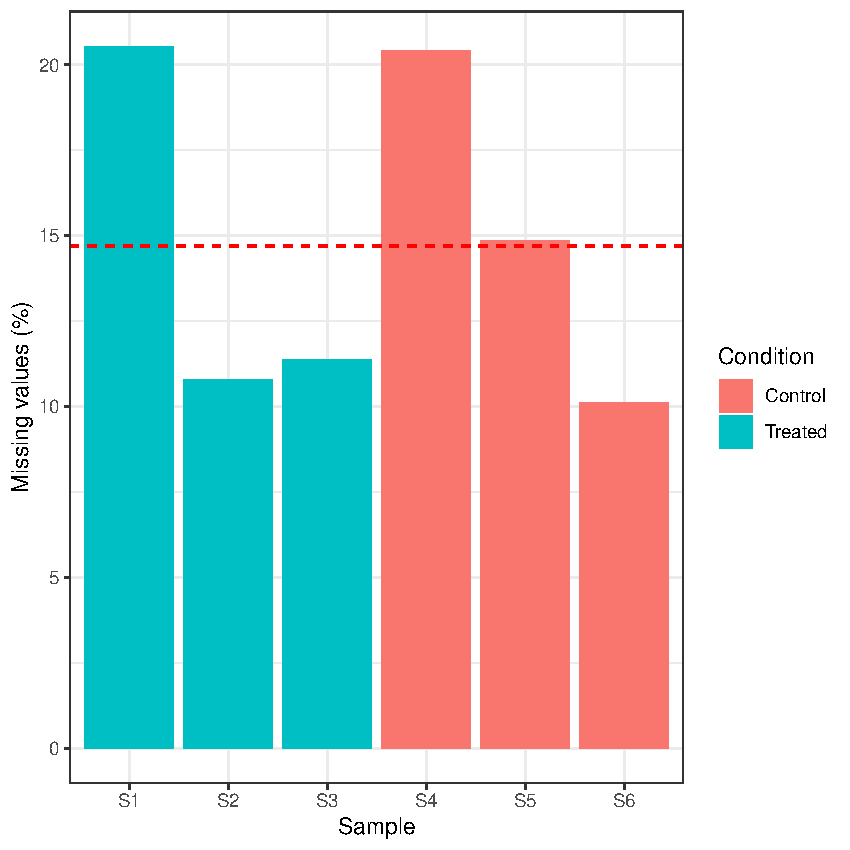
\includegraphics[height=0.4\textheight]{workflow_expressions_files/figure-latex/lfq_missing_data_2-1} \end{center}

Whilst S1 and S4 have a slightly higher proportion of missing values, all of the
samples are within an acceptable range to continue. Again, there is no evidence
of a condition-specific bias in the data.

\subsubsection{Filtering out missing values}\label{filtering-out-missing-values-1}

We next filter out features, here peptides, which comprise 20\% or more missing
values.

\begin{Shaded}
\begin{Highlighting}[]
\DocumentationTok{\#\# Check how many peptides we will remove}
\FunctionTok{which}\NormalTok{(}\FunctionTok{nNA}\NormalTok{(sn\_qf[[}\StringTok{"peptides\_filtered"}\NormalTok{]])}\SpecialCharTok{$}\NormalTok{nNArows}\SpecialCharTok{$}\NormalTok{pNA }\SpecialCharTok{\textgreater{}=} \FloatTok{0.2}\NormalTok{) }\SpecialCharTok{\%\textgreater{}\%}
  \FunctionTok{length}\NormalTok{()}
\end{Highlighting}
\end{Shaded}

\begin{verbatim}
## [1] 4332
\end{verbatim}

\begin{Shaded}
\begin{Highlighting}[]
\DocumentationTok{\#\# Remove peptides with 2 or more NA values}
\NormalTok{sn\_qf }\OtherTok{\textless{}{-}}\NormalTok{ sn\_qf }\SpecialCharTok{\%\textgreater{}\%}
  \FunctionTok{filterNA}\NormalTok{(}\AttributeTok{pNA =} \FloatTok{0.2}\NormalTok{,}
           \AttributeTok{i =} \StringTok{"peptides\_filtered"}\NormalTok{)}
\end{Highlighting}
\end{Shaded}

\subsubsection{Imputation (optional)}\label{imputation-optional-1}

Finally, we check how many missing values remain in the data before making a
decision as to whether imputation is required.

\begin{Shaded}
\begin{Highlighting}[]
\FunctionTok{nNA}\NormalTok{(sn\_qf[[}\StringTok{"peptides\_filtered"}\NormalTok{]])}\SpecialCharTok{$}\NormalTok{nNA}
\end{Highlighting}
\end{Shaded}

\begin{verbatim}
## DataFrame with 1 row and 2 columns
##         nNA       pNA
##   <integer> <numeric>
## 1      2430 0.0298717
\end{verbatim}

There are 2430 missing values remaining.
The presence of proteins with single or low peptide support means that some of
these NA values will likely be propagated upward during aggregation. Whilst NA
values were traditionally problematic during the application of downstream
statistical methods, there are now a number of algorithms that allow statistics
to be completed on data containing missing values. For example, the
(\texttt{MSqRob2}){[}\url{https://www.bioconductor.org/packages/release/bioc/html/msqrob2.html}{]}
\citetext{\citealp[\citet{Goeminne2020}]{Sticker2020}; \citealp{Goeminne2016}} package facilitates statistical
differential expression analysis on datasets without the need for imputation and
functions within the \texttt{QFeatures} infrastructure. Nevertheless, for the purpose of
demonstration, we here choose to impute the raw intensity data.

As eluded to above, the most appropriate method to determine such probable
values is dependent upon why the value is missing, that is whether it is MCAR or
MNAR. Although the optimal imputation method is specific to each dataset,
left-censored methods (e.g.~minimal value approaches, limit of detection) have
proven favorable for data with a high proportion of MNAR values whilst hot deck
methods (e.g.~k-nearest neighbours, random forest, maximum likelihood methods)
are more appropriate when the majority of missing data is MCAR \citep[e.g.,][]{Liu2021, Lazar2016}. Within the \texttt{QFeatures} infrastructure imputation is carried out by
passing the data to the \texttt{impute} function, please see \texttt{?impute} for more
information. To see which imputation methods are supported by this function we
use the following code:

\begin{Shaded}
\begin{Highlighting}[]
\DocumentationTok{\#\# Find out available imputation methods}
\NormalTok{MsCoreUtils}\SpecialCharTok{::}\FunctionTok{imputeMethods}\NormalTok{()}
\end{Highlighting}
\end{Shaded}

\begin{verbatim}
##  [1] "bpca"    "knn"     "QRILC"   "MLE"     "MLE2"    "MinDet"  "MinProb"
##  [8] "min"     "zero"    "mixed"   "nbavg"   "with"    "RF"      "none"
\end{verbatim}

Unfortunately, it is very challenging to determine the reason(s) behind missing
data, and in most cases experiments contain a mixture of MCAR and MNAR. For LFQ
data where little is know about the cause of missing values it is advisable to
use methods optimized for MCAR. Here we will use the baseline k-nearest
neighbours (k-NN) imputation on the raw peptide intensities. Of note, users who
wish to utilize an alternative imputation method should check whether their
selected method has a requirement for normality. If the method requires data to
display a normal distribution, users must log2 transform the data prior to
imputation.

\begin{Shaded}
\begin{Highlighting}[]
\DocumentationTok{\#\# Impute missing values using kNN}
\NormalTok{sn\_qf }\OtherTok{\textless{}{-}} \FunctionTok{impute}\NormalTok{(sn\_qf,}
                \AttributeTok{method =} \StringTok{"knn"}\NormalTok{, }
                \AttributeTok{i =} \StringTok{"peptides\_filtered"}\NormalTok{,}
                \AttributeTok{name =} \StringTok{"peptides\_imputed"}\NormalTok{)}
\end{Highlighting}
\end{Shaded}

Following imputation we check to ensure that the distribution of the data has
not dramatically changed. To do so we create a density plot of the data pre- and
post-imputation.

\begin{Shaded}
\begin{Highlighting}[]
\DocumentationTok{\#\# visualize the impact of imputation}
\FunctionTok{par}\NormalTok{(}\AttributeTok{mfrow =} \FunctionTok{c}\NormalTok{(}\DecValTok{1}\NormalTok{, }\DecValTok{2}\NormalTok{))}

\NormalTok{sn\_qf[[}\StringTok{"peptides\_filtered"}\NormalTok{]] }\SpecialCharTok{\%\textgreater{}\%}
  \FunctionTok{assay}\NormalTok{() }\SpecialCharTok{\%\textgreater{}\%}
  \FunctionTok{log2}\NormalTok{() }\SpecialCharTok{\%\textgreater{}\%}
  \FunctionTok{plotDensities}\NormalTok{(}\AttributeTok{main =} \StringTok{"Pre{-}imputation"}\NormalTok{,}
                \AttributeTok{legend =} \ConstantTok{FALSE}\NormalTok{)}

\NormalTok{sn\_qf[[}\StringTok{"peptides\_imputed"}\NormalTok{]] }\SpecialCharTok{\%\textgreater{}\%}
  \FunctionTok{assay}\NormalTok{() }\SpecialCharTok{\%\textgreater{}\%}
  \FunctionTok{log2}\NormalTok{() }\SpecialCharTok{\%\textgreater{}\%}
  \FunctionTok{plotDensities}\NormalTok{(}\AttributeTok{main =} \StringTok{"Post{-}imputation"}\NormalTok{,}
                \AttributeTok{legend =} \StringTok{"topright"}\NormalTok{)}
\end{Highlighting}
\end{Shaded}

\begin{center}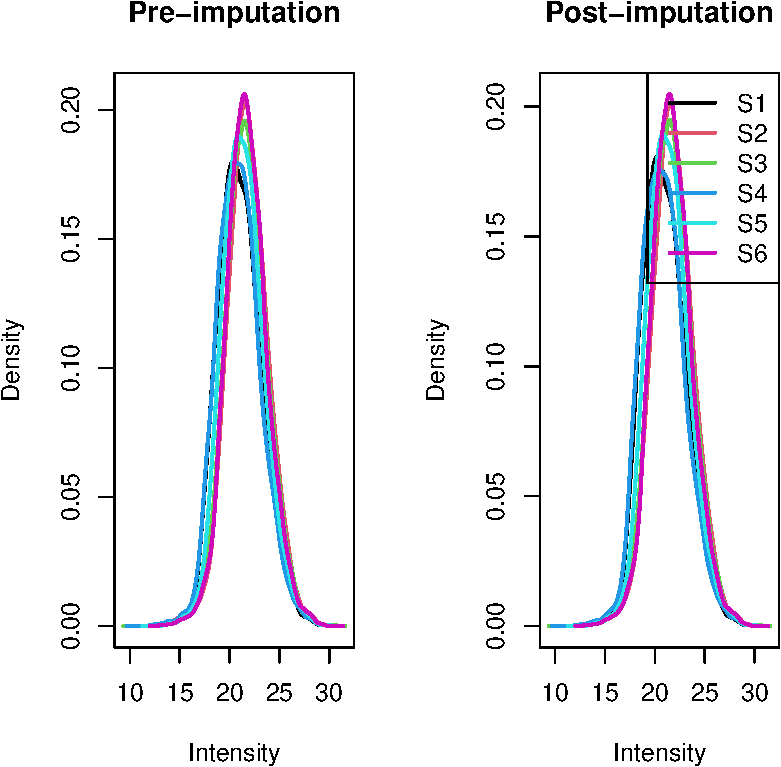
\includegraphics[width=0.8\linewidth]{workflow_expressions_files/figure-latex/lfq_imputation_4-1} \end{center}

From this plot the change in the data appears to be minimal. We can further
validate this by comparing the summary statistics of the data pre- and post-
imputation.

\begin{Shaded}
\begin{Highlighting}[]
\DocumentationTok{\#\# Determine the impact of imputation on summary statistics}
\NormalTok{pre\_imputation\_summary }\OtherTok{\textless{}{-}}\NormalTok{ sn\_qf[[}\StringTok{"peptides\_filtered"}\NormalTok{]] }\SpecialCharTok{\%\textgreater{}\%}
  \FunctionTok{assay}\NormalTok{() }\SpecialCharTok{\%\textgreater{}\%}
  \FunctionTok{longFormat}\NormalTok{() }\SpecialCharTok{\%\textgreater{}\%}
  \FunctionTok{group\_by}\NormalTok{(colname) }\SpecialCharTok{\%\textgreater{}\%}
  \FunctionTok{summarise}\NormalTok{(}\AttributeTok{sum\_intensity =} \FunctionTok{sum}\NormalTok{(value, }\AttributeTok{na.rm =} \ConstantTok{TRUE}\NormalTok{),}
            \AttributeTok{max\_intensity =} \FunctionTok{max}\NormalTok{(value, }\AttributeTok{na.rm =} \ConstantTok{TRUE}\NormalTok{),}
            \AttributeTok{median\_intensity =} \FunctionTok{median}\NormalTok{(value, }\AttributeTok{na.rm =} \ConstantTok{TRUE}\NormalTok{))}

\NormalTok{post\_imputation\_summary }\OtherTok{\textless{}{-}}\NormalTok{ sn\_qf[[}\StringTok{"peptides\_imputed"}\NormalTok{]] }\SpecialCharTok{\%\textgreater{}\%}
  \FunctionTok{assay}\NormalTok{() }\SpecialCharTok{\%\textgreater{}\%}
  \FunctionTok{longFormat}\NormalTok{() }\SpecialCharTok{\%\textgreater{}\%}
  \FunctionTok{group\_by}\NormalTok{(colname) }\SpecialCharTok{\%\textgreater{}\%}
  \FunctionTok{summarise}\NormalTok{(}\AttributeTok{sum\_intensity =} \FunctionTok{sum}\NormalTok{(value, }\AttributeTok{na.rm =} \ConstantTok{TRUE}\NormalTok{),}
            \AttributeTok{max\_intensity =} \FunctionTok{max}\NormalTok{(value, }\AttributeTok{na.rm =} \ConstantTok{TRUE}\NormalTok{),}
            \AttributeTok{median\_intensity =} \FunctionTok{median}\NormalTok{(value, }\AttributeTok{na.rm =} \ConstantTok{TRUE}\NormalTok{))}

\FunctionTok{print}\NormalTok{(pre\_imputation\_summary)}
\end{Highlighting}
\end{Shaded}

\begin{verbatim}
## # A tibble: 6 x 4
##   colname sum_intensity max_intensity median_intensity
##   <fct>           <dbl>         <dbl>            <dbl>
## 1 S1       98618011197.   1477162278.         1950392.
## 2 S2      155288272302.   1678988256.         3567233.
## 3 S3      145083815203.   1804842981.         3255696.
## 4 S4       94532147208.   1087946291.         1880489.
## 5 S5      121223290798.   1307181986          2511748.
## 6 S6      143149276808.   1608003894.         3288965.
\end{verbatim}

\begin{Shaded}
\begin{Highlighting}[]
\FunctionTok{print}\NormalTok{(post\_imputation\_summary)}
\end{Highlighting}
\end{Shaded}

\begin{verbatim}
## # A tibble: 6 x 4
##   colname sum_intensity max_intensity median_intensity
##   <fct>           <dbl>         <dbl>            <dbl>
## 1 S1       99501169413.   1477162278.         1814576.
## 2 S2      155691649219.   1678988256.         3493145.
## 3 S3      145325835653.   1804842981.         3210018.
## 4 S4       95867237989.   1087946291.         1726081.
## 5 S5      121738595609.   1307181986          2446493.
## 6 S6      143619358837.   1608003894.         3216396.
\end{verbatim}

Comparison of the two tables reveals minimal change within the data. However, we
find that S1 and S4 display greater differences between pre- and post-imputation
statistics because of the higher number of missing values which required
imputation.

\subsection{Logarithmic transformation of quantitative data}\label{logarithmic-transformation-of-quantitative-data-1}

In the following code chunk we log2 transform the peptide-level data to generate
a near-normal distribution within the quantitative data. This is necessary prior
to the use of \texttt{robustSummary} aggregation.

\begin{Shaded}
\begin{Highlighting}[]
\DocumentationTok{\#\# log2 transform the quantitative data}
\NormalTok{sn\_qf }\OtherTok{\textless{}{-}} \FunctionTok{logTransform}\NormalTok{(}\AttributeTok{object =}\NormalTok{ sn\_qf,}
                      \AttributeTok{base =} \DecValTok{2}\NormalTok{,}
                      \AttributeTok{i =} \StringTok{"peptides\_imputed"}\NormalTok{,}
                      \AttributeTok{name =} \StringTok{"log\_peptides"}\NormalTok{)}

\DocumentationTok{\#\# Verify}
\NormalTok{sn\_qf}
\end{Highlighting}
\end{Shaded}

\begin{verbatim}
## An instance of class QFeatures containing 4 assays:
##  [1] peptides_raw: SummarizedExperiment with 23375 rows and 6 columns 
##  [2] peptides_filtered: SummarizedExperiment with 13558 rows and 6 columns 
##  [3] peptides_imputed: SummarizedExperiment with 13558 rows and 6 columns 
##  [4] log_peptides: SummarizedExperiment with 13558 rows and 6 columns
\end{verbatim}

\subsection{Aggregation of peptide to protein}\label{aggregation-of-peptide-to-protein}

Now that we are happy with the peptide-level data, we aggregate upward to
proteins using the \texttt{aggregateFeatures} function.

\begin{Shaded}
\begin{Highlighting}[]
\DocumentationTok{\#\# Aggregate peptide to protein}
\NormalTok{sn\_qf }\OtherTok{\textless{}{-}} \FunctionTok{aggregateFeatures}\NormalTok{(sn\_qf,}
                           \AttributeTok{i =} \StringTok{"log\_peptides"}\NormalTok{,}
                           \AttributeTok{fcol =} \StringTok{"Master.Protein.Accessions"}\NormalTok{,}
                           \AttributeTok{name =} \StringTok{"log\_proteins"}\NormalTok{,}
                           \AttributeTok{fun =}\NormalTok{ MsCoreUtils}\SpecialCharTok{::}\NormalTok{robustSummary,}
                           \AttributeTok{na.rm =} \ConstantTok{TRUE}\NormalTok{)}
\end{Highlighting}
\end{Shaded}

\begin{verbatim}
## Your row data contain missing values. Please read the relevant
## section(s) in the aggregateFeatures manual page regarding the effects
## of missing values on data aggregation.
\end{verbatim}

\begin{Shaded}
\begin{Highlighting}[]
\DocumentationTok{\#\# Verify}
\NormalTok{sn\_qf}
\end{Highlighting}
\end{Shaded}

\begin{verbatim}
## An instance of class QFeatures containing 5 assays:
##  [1] peptides_raw: SummarizedExperiment with 23375 rows and 6 columns 
##  [2] peptides_filtered: SummarizedExperiment with 13558 rows and 6 columns 
##  [3] peptides_imputed: SummarizedExperiment with 13558 rows and 6 columns 
##  [4] log_peptides: SummarizedExperiment with 13558 rows and 6 columns 
##  [5] log_proteins: SummarizedExperiment with 2760 rows and 6 columns
\end{verbatim}

\subsection{Normalization of quantitative data}\label{normalization-of-quantitative-data-1}

Finally, we complete the data processing by normalizing quantitation between
samples. This is done using the \texttt{"center.median"} method via the \texttt{normalize}
function.

\begin{Shaded}
\begin{Highlighting}[]
\DocumentationTok{\#\# normalize protein{-}level quantitation data}
\NormalTok{sn\_qf }\OtherTok{\textless{}{-}} \FunctionTok{normalize}\NormalTok{(sn\_qf,}
                   \AttributeTok{i =} \StringTok{"log\_proteins"}\NormalTok{,}
                   \AttributeTok{name =} \StringTok{"log\_norm\_proteins"}\NormalTok{,}
                   \AttributeTok{method =} \StringTok{"center.median"}\NormalTok{)}

\DocumentationTok{\#\# Verify}
\NormalTok{sn\_qf}
\end{Highlighting}
\end{Shaded}

\begin{verbatim}
## An instance of class QFeatures containing 6 assays:
##  [1] peptides_raw: SummarizedExperiment with 23375 rows and 6 columns 
##  [2] peptides_filtered: SummarizedExperiment with 13558 rows and 6 columns 
##  [3] peptides_imputed: SummarizedExperiment with 13558 rows and 6 columns 
##  [4] log_peptides: SummarizedExperiment with 13558 rows and 6 columns 
##  [5] log_proteins: SummarizedExperiment with 2760 rows and 6 columns 
##  [6] log_norm_proteins: SummarizedExperiment with 2760 rows and 6 columns
\end{verbatim}

The final dataset is comprised of 2760 protein
groups. We will save the protein-level \texttt{SummarizedExperiment} file as well as
exporting the final \texttt{QFeatures} object.

\begin{Shaded}
\begin{Highlighting}[]
\DocumentationTok{\#\# Save protein{-}level SE}
\NormalTok{sn\_proteins }\OtherTok{\textless{}{-}}\NormalTok{ sn\_qf[[}\StringTok{"log\_norm\_proteins"}\NormalTok{]]}

\DocumentationTok{\#\# Export TMT final QFeatures object}
\FunctionTok{save}\NormalTok{(sn\_qf, }\AttributeTok{file =} \StringTok{"sn\_qf.rda"}\NormalTok{)}
\end{Highlighting}
\end{Shaded}

\section{Exploration of protein data}\label{exploration-of-protein-data}

Having described the processing steps for quantitative proteomics data, we next
demonstrate how to explore the protein-level data prior to statistical analysis.
For this we will utilize the TMT-labelled cell pellet dataset since it contains
a greater number of proteins.

\subsection{Correlation plots}\label{correlation-plots}

We will first generate correlation plots between pairs of samples. To do this we
use the \href{https://cran.r-project.org/web/packages/corrplot/vignettes/corrplot-intro.html}{\texttt{corrplot}}
package to calculate and plot the Pearson's correlation coefficient between each
sample pair. The \texttt{cor} function within the \texttt{corrplot} package will create a
correlation matrix but requires a \texttt{data.frame}, \texttt{matrix} or a \texttt{vector} of class
\texttt{numeric} as input. To convert the \texttt{QFeatures} \texttt{assay} data into a \texttt{data.frame}
we use the \texttt{as.data.frame} function.

\begin{Shaded}
\begin{Highlighting}[]
\DocumentationTok{\#\# Convert TMT CP protein assay into a dataframe}
\NormalTok{prot\_df }\OtherTok{\textless{}{-}}\NormalTok{ cp\_qf[[}\StringTok{"log\_norm\_proteins"}\NormalTok{]] }\SpecialCharTok{\%\textgreater{}\%}
  \FunctionTok{assay}\NormalTok{() }\SpecialCharTok{\%\textgreater{}\%}
  \FunctionTok{as.data.frame}\NormalTok{()}

\DocumentationTok{\#\# Calculate a correlation matrix between samples}
\NormalTok{corr\_matrix }\OtherTok{\textless{}{-}} \FunctionTok{cor}\NormalTok{(prot\_df,}
                   \AttributeTok{method =} \StringTok{"pearson"}\NormalTok{,}
                   \AttributeTok{use =} \StringTok{"pairwise.complete.obs"}\NormalTok{)}

\FunctionTok{print}\NormalTok{(corr\_matrix)}
\end{Highlighting}
\end{Shaded}

\begin{verbatim}
##           S5        S2        S1        S4        S6        S3
## S5 1.0000000 0.9540226 0.9634202 0.9821489 0.9927946 0.9558386
## S2 0.9540226 1.0000000 0.9862036 0.9207314 0.9508941 0.9886243
## S1 0.9634202 0.9862036 1.0000000 0.9451292 0.9637123 0.9926604
## S4 0.9821489 0.9207314 0.9451292 1.0000000 0.9864988 0.9348920
## S6 0.9927946 0.9508941 0.9637123 0.9864988 1.0000000 0.9557268
## S3 0.9558386 0.9886243 0.9926604 0.9348920 0.9557268 1.0000000
\end{verbatim}

Now we can visualize the correlation data using pairwise scatter plots and a
correlation heat map.

\begin{Shaded}
\begin{Highlighting}[]
\DocumentationTok{\#\# Plot correlation between two samples {-} S1 and S2 used as example}
\NormalTok{prot\_df }\SpecialCharTok{\%\textgreater{}\%}
  \FunctionTok{ggplot}\NormalTok{(}\FunctionTok{aes}\NormalTok{(}\AttributeTok{x =} \StringTok{\textasciigrave{}}\AttributeTok{S1}\StringTok{\textasciigrave{}}\NormalTok{, }\AttributeTok{y =} \StringTok{\textasciigrave{}}\AttributeTok{S2}\StringTok{\textasciigrave{}}\NormalTok{)) }\SpecialCharTok{+}
  \FunctionTok{geom\_point}\NormalTok{(}\AttributeTok{colour =} \StringTok{"grey45"}\NormalTok{, }\AttributeTok{size =} \FloatTok{0.5}\NormalTok{) }\SpecialCharTok{+}
  \FunctionTok{geom\_abline}\NormalTok{(}\AttributeTok{intercept =} \DecValTok{0}\NormalTok{, }\AttributeTok{slope =} \DecValTok{1}\NormalTok{) }\SpecialCharTok{+}
  \FunctionTok{theme}\NormalTok{(}\AttributeTok{panel.grid.major =} \FunctionTok{element\_blank}\NormalTok{(), }
        \AttributeTok{panel.grid.minor =} \FunctionTok{element\_blank}\NormalTok{(),}
        \AttributeTok{plot.background =} \FunctionTok{element\_rect}\NormalTok{(}\AttributeTok{fill =} \StringTok{"white"}\NormalTok{),}
        \AttributeTok{panel.background =} \FunctionTok{element\_rect}\NormalTok{(}\AttributeTok{fill =} \StringTok{"white"}\NormalTok{),}
        \AttributeTok{axis.title.x =} \FunctionTok{element\_text}\NormalTok{(}\AttributeTok{size =} \DecValTok{15}\NormalTok{, }\AttributeTok{vjust =} \SpecialCharTok{{-}}\DecValTok{2}\NormalTok{),}
        \AttributeTok{axis.title.y =} \FunctionTok{element\_text}\NormalTok{(}\AttributeTok{size =} \DecValTok{15}\NormalTok{, }\AttributeTok{vjust =} \DecValTok{3}\NormalTok{),}
        \AttributeTok{axis.text.x =} \FunctionTok{element\_text}\NormalTok{(}\AttributeTok{size =} \DecValTok{12}\NormalTok{, }\AttributeTok{vjust =} \SpecialCharTok{{-}}\DecValTok{1}\NormalTok{),}
        \AttributeTok{axis.text.y =} \FunctionTok{element\_text}\NormalTok{(}\AttributeTok{size =} \DecValTok{12}\NormalTok{),}
        \AttributeTok{axis.line =} \FunctionTok{element\_line}\NormalTok{(}\AttributeTok{linewidth =} \FloatTok{0.5}\NormalTok{, }\AttributeTok{colour =} \StringTok{"black"}\NormalTok{),}
        \AttributeTok{plot.margin =} \FunctionTok{margin}\NormalTok{(}\DecValTok{10}\NormalTok{, }\DecValTok{10}\NormalTok{, }\DecValTok{10}\NormalTok{, }\DecValTok{10}\NormalTok{)) }\SpecialCharTok{+}
  \FunctionTok{xlim}\NormalTok{(}\SpecialCharTok{{-}}\FloatTok{7.5}\NormalTok{, }\DecValTok{5}\NormalTok{) }\SpecialCharTok{+}
  \FunctionTok{ylim}\NormalTok{(}\SpecialCharTok{{-}}\FloatTok{7.5}\NormalTok{, }\DecValTok{5}\NormalTok{) }\SpecialCharTok{+}
  \FunctionTok{labs}\NormalTok{(}\AttributeTok{x =} \StringTok{"log2(abundance S1)"}\NormalTok{, }\AttributeTok{y =} \StringTok{"log2(abundance S2)"}\NormalTok{) }\SpecialCharTok{+}
  \FunctionTok{coord\_fixed}\NormalTok{(}\AttributeTok{ratio =} \DecValTok{1}\NormalTok{)}
\end{Highlighting}
\end{Shaded}

\begin{center}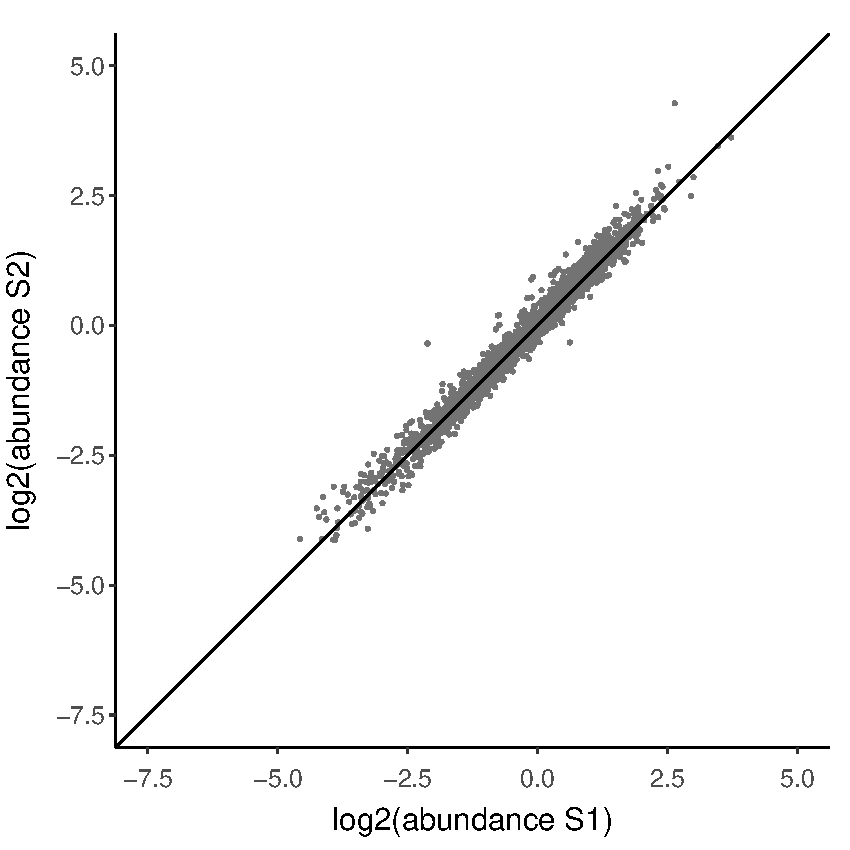
\includegraphics[height=0.3\textheight]{workflow_expressions_files/figure-latex/correlation_plot_2-1} \end{center}

\begin{Shaded}
\begin{Highlighting}[]
\DocumentationTok{\#\# Create colour palette for continuum}
\NormalTok{col }\OtherTok{\textless{}{-}} \FunctionTok{colorRampPalette}\NormalTok{(}\FunctionTok{c}\NormalTok{(}\StringTok{"\#BB4444"}\NormalTok{, }\StringTok{"\#EE9988"}\NormalTok{, }\StringTok{"\#FFFFFF"}\NormalTok{,}
                          \StringTok{"\#77AADD"}\NormalTok{, }\StringTok{"\#4477AA"}\NormalTok{))}

\DocumentationTok{\#\# Plot all pairwise correlations}
\NormalTok{prot\_df }\SpecialCharTok{\%\textgreater{}\%}
  \FunctionTok{cor}\NormalTok{(}\AttributeTok{method =} \StringTok{"pearson"}\NormalTok{, }
      \AttributeTok{use =} \StringTok{"pairwise.complete.obs"}\NormalTok{) }\SpecialCharTok{\%\textgreater{}\%}
  \FunctionTok{corrplot}\NormalTok{(}\AttributeTok{method =} \StringTok{"color"}\NormalTok{,}
           \AttributeTok{col =} \FunctionTok{col}\NormalTok{(}\DecValTok{200}\NormalTok{), }
           \AttributeTok{type =} \StringTok{"upper"}\NormalTok{, }
           \AttributeTok{addCoef.col =} \StringTok{"white"}\NormalTok{,}
           \AttributeTok{diag =} \ConstantTok{FALSE}\NormalTok{, }
           \AttributeTok{tl.col =} \StringTok{"black"}\NormalTok{, }
           \AttributeTok{tl.srt =} \DecValTok{45}\NormalTok{, }
           \AttributeTok{outline =} \ConstantTok{TRUE}\NormalTok{)}
\end{Highlighting}
\end{Shaded}

\begin{center}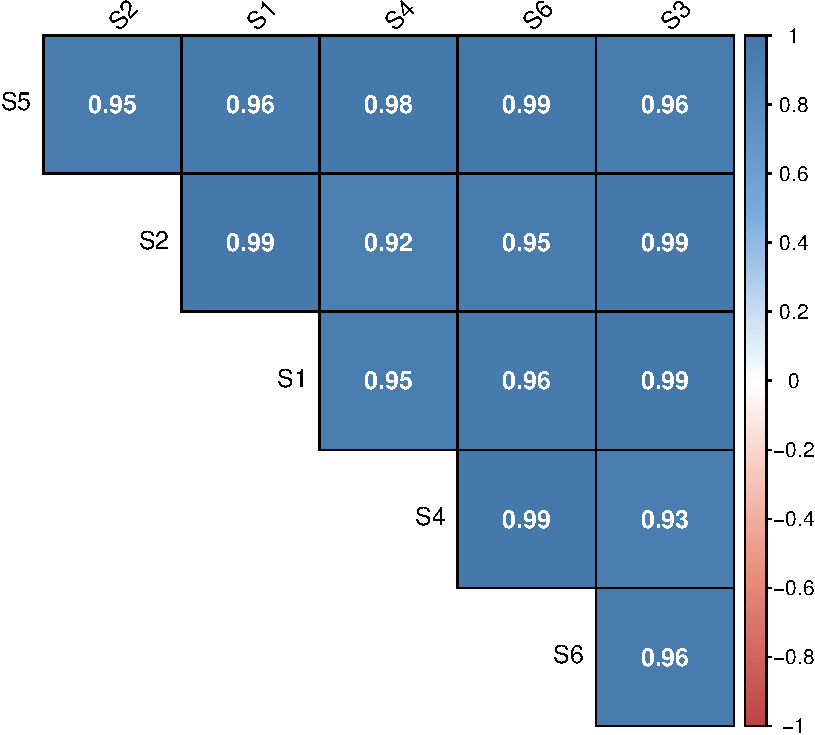
\includegraphics[height=0.3\textheight]{workflow_expressions_files/figure-latex/correlation_plot_3-1} \end{center}

From these plots we can see that all replicate pairs have a Pearson's correlation
coefficient \textgreater0.98 whilst the correlation between pairs of control and treated
samples is somewhat lower. Users may interpret this information as an early
indication that some proteins may be differentially abundant between the two
groups.

Of note, whilst correlation is widely applied as a measure of reproducibility,
users are reminded that correlation coefficients alone are not informative of
reproducibility \citep{simply_stats, Bunting2019}. This is especially true for
expression proteomics data in which high correlation values are likely due to
the majority of proteins remaining at similar levels regardless of cellular
perturbation. Users are directed to \citep{Darbani2014} for additional information
regarding how to determine the calculation of experimental reproducibility.

\subsection{Principal Component Analysis}\label{principal-component-analysis}

Principal Component Analysis (PCA) is a dimensionality reduction method which
aims to simplify complex datasets and facilitate the visualization of
multi-dimensional data. Here we use the \texttt{prcomp} function from the
\href{https://stat.ethz.ch/R-manual/R-devel/library/stats/html/00Index.html}{\texttt{stats}}
package to perform the PCA. Since PCA does not accept missing values and we did
not impute the TMT data, the \texttt{filterNA} function can be used to remove any
missing values that may be present in the protein-level data. We then extract
and transpose the assay data before passing it to the \texttt{prcomp} function to carry
out PCA.

\begin{Shaded}
\begin{Highlighting}[]
\DocumentationTok{\#\# Carry out principal component analysis}
\NormalTok{prot\_pca }\OtherTok{\textless{}{-}}\NormalTok{ cp\_qf[[}\StringTok{"log\_norm\_proteins"}\NormalTok{]] }\SpecialCharTok{\%\textgreater{}\%}
  \FunctionTok{filterNA}\NormalTok{() }\SpecialCharTok{\%\textgreater{}\%}
  \FunctionTok{assay}\NormalTok{() }\SpecialCharTok{\%\textgreater{}\%}
  \FunctionTok{t}\NormalTok{() }\SpecialCharTok{\%\textgreater{}\%}
  \FunctionTok{prcomp}\NormalTok{(}\AttributeTok{scale =} \ConstantTok{TRUE}\NormalTok{, }\AttributeTok{center =} \ConstantTok{TRUE}\NormalTok{)}
\end{Highlighting}
\end{Shaded}

We can get an idea of the outcome of the PCA by running the \texttt{summary} function
on the results of the PCA.

\begin{Shaded}
\begin{Highlighting}[]
\DocumentationTok{\#\# Get a summary of the PCA}
\FunctionTok{summary}\NormalTok{(prot\_pca)}
\end{Highlighting}
\end{Shaded}

\begin{verbatim}
## Importance of components:
##                           PC1     PC2     PC3      PC4     PC5       PC6
## Standard deviation     42.035 26.5522 18.1232 14.97317 14.3323 4.334e-14
## Proportion of Variance  0.547  0.2183  0.1017  0.06941  0.0636 0.000e+00
## Cumulative Proportion   0.547  0.7653  0.8670  0.93640  1.0000 1.000e+00
\end{verbatim}

Finally, we create a PCA plot. For additional PCA exploration and visualization
tools users are directed to the \href{https://cran.r-project.org/web/packages/factoextra/index.html}{\texttt{factoextra} package}.

\begin{Shaded}
\begin{Highlighting}[]
\DocumentationTok{\#\# Generate dataframe of each sample\textquotesingle{}s PCA results}
\NormalTok{pca\_df }\OtherTok{\textless{}{-}} \FunctionTok{as.data.frame}\NormalTok{(prot\_pca}\SpecialCharTok{$}\NormalTok{x)}

\DocumentationTok{\#\# Annotate samples with their corresponding condition}
\NormalTok{pca\_df}\SpecialCharTok{$}\NormalTok{condition }\OtherTok{\textless{}{-}}\NormalTok{ cp\_qf[[}\StringTok{"psms\_raw"}\NormalTok{]]}\SpecialCharTok{$}\NormalTok{condition}

\DocumentationTok{\#\# Generate a PCA plot using PC1 and PC2}
\NormalTok{pca\_df }\SpecialCharTok{\%\textgreater{}\%}
  \FunctionTok{ggplot}\NormalTok{(}\FunctionTok{aes}\NormalTok{(}\AttributeTok{x =}\NormalTok{ PC1, }\AttributeTok{y =}\NormalTok{ PC2, }\AttributeTok{colour =}\NormalTok{ condition)) }\SpecialCharTok{+}
  \FunctionTok{geom\_point}\NormalTok{(}\AttributeTok{size =} \DecValTok{4}\NormalTok{) }\SpecialCharTok{+}
  \FunctionTok{scale\_color\_brewer}\NormalTok{(}\AttributeTok{palette =} \StringTok{"Set2"}\NormalTok{) }\SpecialCharTok{+}
  \FunctionTok{labs}\NormalTok{(}\AttributeTok{colour =} \StringTok{"Condition"}\NormalTok{) }\SpecialCharTok{+}
  \FunctionTok{geom\_hline}\NormalTok{(}\AttributeTok{yintercept =} \DecValTok{0}\NormalTok{, }\AttributeTok{linetype =} \StringTok{"dashed"}\NormalTok{) }\SpecialCharTok{+}
  \FunctionTok{geom\_vline}\NormalTok{(}\AttributeTok{xintercept =} \DecValTok{0}\NormalTok{, }\AttributeTok{linetype =} \StringTok{"dashed"}\NormalTok{) }\SpecialCharTok{+}
  \FunctionTok{guides}\NormalTok{(}\AttributeTok{colour =} \FunctionTok{guide\_legend}\NormalTok{(}\AttributeTok{override.aes =} \FunctionTok{list}\NormalTok{(}\AttributeTok{size =} \DecValTok{3}\NormalTok{))) }\SpecialCharTok{+}
  \FunctionTok{labs}\NormalTok{(}\AttributeTok{x =} \StringTok{"PC1"}\NormalTok{, }\AttributeTok{y =} \StringTok{"PC2"}\NormalTok{) }\SpecialCharTok{+}
  \FunctionTok{ggtitle}\NormalTok{(}\StringTok{"Protein{-}level PCA plot"}\NormalTok{) }\SpecialCharTok{+}
  \FunctionTok{xlim}\NormalTok{(}\SpecialCharTok{{-}}\DecValTok{100}\NormalTok{, }\DecValTok{100}\NormalTok{) }\SpecialCharTok{+}
  \FunctionTok{ylim}\NormalTok{(}\SpecialCharTok{{-}}\DecValTok{100}\NormalTok{, }\DecValTok{100}\NormalTok{) }\SpecialCharTok{+}
  \FunctionTok{coord\_fixed}\NormalTok{(}\AttributeTok{ratio =} \DecValTok{1}\NormalTok{) }\SpecialCharTok{+}
  \FunctionTok{theme\_bw}\NormalTok{()}
\end{Highlighting}
\end{Shaded}

\begin{center}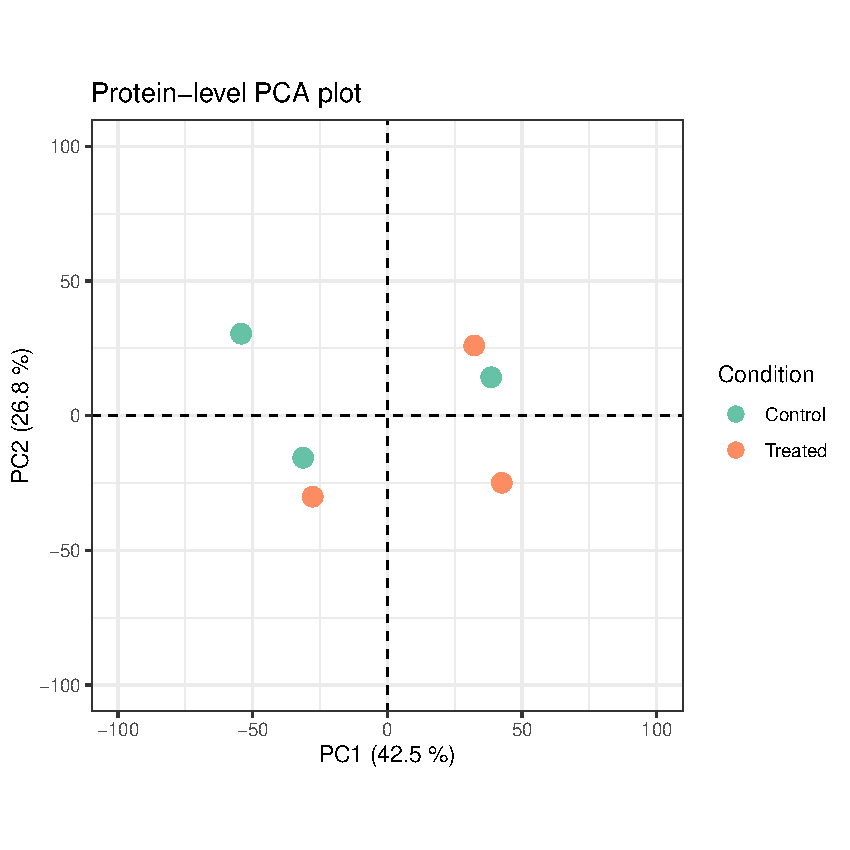
\includegraphics[height=0.4\textheight]{workflow_expressions_files/figure-latex/protein_pca_plot-1} \end{center}

\subsubsection{Exploring potential batch effects}\label{exploring-potential-batch-effects}

Before carrying out differential expression analysis, it is first necessary to
explore the presence of batch effects within the data. Batch effects are derived
from non-biological factors which impact the experimental data. These include
reagents, instrumentation, personnel and laboratory conditions. In most cases
the increased variation caused by batch effects will lead to reduced downstream
statistical power. On the other hand, if correlated with the experimental sub-
groups, batch effects can also lead to confounded results and the incorrect
biological interpretation of differential expression \citep{Leek2010}.

Given that the use-case data was derived from a small experiment with only six
samples and a single TMTplex, there are minimal batch effects to explore here.
For users analyzing larger experiments completed over long period of time, across
several laboratories/individuals, or using multiple TMTplex reagents, it is
advisable to annotate the PCA plot with all potential batch factors. If data is
found to cluster based on any of these factors, batch effects should be
incorporated into downstream analyses. For example, users can apply the
\href{https://rdrr.io/bioc/limma/man/removeBatchEffect.html}{\texttt{removeBatchEffect}}
function from the \texttt{limma} package.

\section{Discovery and biological interpretation of differentially abundant proteins}\label{discovery-and-biological-interpretation-of-differentially-abundant-proteins}

The last section of this workflow demonstrates how to gain biological insights
from the resulting list of proteins. Again we will utilize the TMT-labelled cell
pellet data, although the process would be exactly the same for the LFQ
supernatant protein list. Users are reminded that although referred to as
differential `expression' analysis, abundance is determined by both protein
synthesis and degradation.

Given that there are a number of Bioconductor packages available for each of the
remaining steps (statistical analysis and interpretation), users are prompted to
install packages at the where required, at the beginning of each step.

\subsection{Extracting and organising protein-level data}\label{extracting-and-organising-protein-level-data}

We first extract the protein-level \texttt{SummarizedExperiment} from the cell pellet
TMT \texttt{QFeatures} object and specify the study factors. Here we are interested in
discovering differences between conditions, control and treated. As well as
assigning these conditions to each sample, we can define the control group as the
reference level such that differential abundance is reported relative to the
control. This means that when we get the results of the statistical analysis,
`upregulated' will refer to increased abundance in treated cells relative to
control controls.

\begin{Shaded}
\begin{Highlighting}[]
\DocumentationTok{\#\# Extract protein{-}level data and associated colData}
\NormalTok{cp\_proteins }\OtherTok{\textless{}{-}}\NormalTok{ cp\_qf[[}\StringTok{"log\_norm\_proteins"}\NormalTok{]]}
\FunctionTok{colData}\NormalTok{(cp\_proteins) }\OtherTok{\textless{}{-}} \FunctionTok{colData}\NormalTok{(cp\_qf[[}\StringTok{"log\_norm\_proteins"}\NormalTok{]])}

\DocumentationTok{\#\# Create factor of interest}
\NormalTok{cp\_proteins}\SpecialCharTok{$}\NormalTok{condition }\OtherTok{\textless{}{-}} \FunctionTok{factor}\NormalTok{(cp\_proteins}\SpecialCharTok{$}\NormalTok{condition)}

\DocumentationTok{\#\# Check which level of the factor is the reference level and correct}
\NormalTok{cp\_proteins}\SpecialCharTok{$}\NormalTok{condition}
\end{Highlighting}
\end{Shaded}

\begin{verbatim}
## [1] Control Treated Treated Control Control Treated
## Levels: Control Treated
\end{verbatim}

\begin{Shaded}
\begin{Highlighting}[]
\NormalTok{cp\_proteins}\SpecialCharTok{$}\NormalTok{condition }\OtherTok{\textless{}{-}} \FunctionTok{relevel}\NormalTok{(cp\_proteins}\SpecialCharTok{$}\NormalTok{condition, }\AttributeTok{ref =} \StringTok{"Control"}\NormalTok{)}
\end{Highlighting}
\end{Shaded}

\subsection{\texorpdfstring{Differential expression analysis using \texttt{limma}}{Differential expression analysis using limma}}\label{differential-expression-analysis-using-limma}

Bioconductor contains several packages dedicated to the statistical analysis of
proteomics data. For example, \href{https://bioconductor.org/packages/3.15/bioc/html/MSstats.html}{\texttt{MSstats}}
and \href{https://bioconductor.org/packages/3.15/bioc/html/MSstatsTMT.html}{\texttt{MSstatsTMT}}
can be used to determine differential protein expression within both DDA and DIA
datasets for LFQ and TMT, respectively \citep{Choi2014, Huang2020}. Of note,
\texttt{MSstatsTMT} includes additional functionality for dealing with larger,
multi-plexed TMT experiments. For LFQ experiments,
\href{https://bioconductor.org/packages/release/bioc/html/proDA.html}{\texttt{proDA}},
\href{https://rdrr.io/github/wolski/prolfqua/}{\texttt{prolfqua}} and
\href{https://www.bioconductor.org/packages/release/bioc/html/msqrob2.html}{\texttt{MSqRob2}}
can be utilized, among others \citep{Goeminne2020, Wolski2023}. Here, we will use the
\href{https://bioconductor.org/packages/release/bioc/html/limma.html}{\texttt{limma}}
package \citep{Ritchie2015}. \texttt{limma} is widely used for the analysis of large omics
datasets and has several models that allow differential abundance to be assessed
in multifactorial experiments. This is useful because it allows multiple factors,
including TMTplex, to be integrated into the model itself, thus minimising the
effects of confounding factors. In this example we will apply \texttt{limma}'s
empirical Bayes moderated t-test, a method that is appropriate for small sample
sizes \citep{Smyth2004}.

We first use the \texttt{model.matrix} function to create a matrix in which each of the
samples are annotated based on the factors we wish to model, here the condition
group. This ultimately defines the `design' of the model, that is how the
samples are distributed between the groups of interest. We then fit a linear
model to the abundance data of each protein by passing the data and model design
matrix to the \texttt{lmFit} function. Finally, we update the estimated standard error
for each model coefficient using the \texttt{eBayes} function. This function borrows
information across features, here proteins, to shift the per-protein variance
estimates towards an expected value based on the variance estimates of other
proteins with similar mean intensity. This empirical Bayes technique has been
shown to reduce the number of false positives for proteins with small variances
as well as increase the power of detection for differentially abundant proteins
with larger variances \citep{Phipson2016}. Further, we use the \texttt{trend\ =\ TRUE} argument
when passing the \texttt{eBayes} function so that an intensity-dependent trend can be
fitted to the prior variances. For more information about the \texttt{limma} trend
method users are directed to \citep{Law2014}.

\begin{Shaded}
\begin{Highlighting}[]
\DocumentationTok{\#\# Design a matrix containing all of the factors we wish to model the effects of}
\NormalTok{model\_design }\OtherTok{\textless{}{-}} \FunctionTok{model.matrix}\NormalTok{(}\SpecialCharTok{\textasciitilde{}}\NormalTok{ cp\_proteins}\SpecialCharTok{$}\NormalTok{condition)}

\DocumentationTok{\#\# Verify}
\FunctionTok{print}\NormalTok{(model\_design)}
\end{Highlighting}
\end{Shaded}

\begin{verbatim}
##   (Intercept) cp_proteins$conditionTreated
## 1           1                            0
## 2           1                            1
## 3           1                            1
## 4           1                            0
## 5           1                            0
## 6           1                            1
## attr(,"assign")
## [1] 0 1
## attr(,"contrasts")
## attr(,"contrasts")$`cp_proteins$condition`
## [1] "contr.treatment"
\end{verbatim}

\begin{Shaded}
\begin{Highlighting}[]
\DocumentationTok{\#\# Create a linear model using this design}
\NormalTok{fitted\_lm }\OtherTok{\textless{}{-}}\NormalTok{ cp\_proteins }\SpecialCharTok{\%\textgreater{}\%}
  \FunctionTok{assay}\NormalTok{() }\SpecialCharTok{\%\textgreater{}\%}
  \FunctionTok{lmFit}\NormalTok{(}\AttributeTok{design =}\NormalTok{ model\_design)}
  
\DocumentationTok{\#\# Update the model based on Limma eBayes algorithm}
\NormalTok{fitted\_lm }\OtherTok{\textless{}{-}} \FunctionTok{eBayes}\NormalTok{(}\AttributeTok{fit =}\NormalTok{ fitted\_lm,}
                    \AttributeTok{trend =} \ConstantTok{TRUE}\NormalTok{)}

\DocumentationTok{\#\# Save results of the test}
\NormalTok{limma\_results }\OtherTok{\textless{}{-}} \FunctionTok{topTable}\NormalTok{(}\AttributeTok{fit =}\NormalTok{ fitted\_lm,}
                          \AttributeTok{coef =} \StringTok{"cp\_proteins$conditionTreated"}\NormalTok{,}
                          \AttributeTok{adjust.method =} \StringTok{"BH"}\NormalTok{,}
                          \AttributeTok{number =} \ConstantTok{Inf}\NormalTok{) }\SpecialCharTok{\%\textgreater{}\%}
  \FunctionTok{rownames\_to\_column}\NormalTok{(}\StringTok{"Protein"}\NormalTok{) }\SpecialCharTok{\%\textgreater{}\%}
  \FunctionTok{as\_tibble}\NormalTok{() }\SpecialCharTok{\%\textgreater{}\%}
  \FunctionTok{mutate}\NormalTok{(}\AttributeTok{TP =} \FunctionTok{grepl}\NormalTok{(}\StringTok{"ups"}\NormalTok{, Protein))}
\end{Highlighting}
\end{Shaded}

Having applied the model to the data, we need to verify that this model was
appropriate and that the statistical assumptions were met. To do this we first
generate an SA plot using the \texttt{plotSA} function within \texttt{limma}. An SA plot shows
the log2 residual standard deviation (sigma) against log average abundance and
is a simple way to visualize the trend that has been fitted to the data.

\begin{Shaded}
\begin{Highlighting}[]
\DocumentationTok{\#\# Plot residual SD against average log abundance}
\FunctionTok{plotSA}\NormalTok{(fitted\_lm,}
       \AttributeTok{xlab =} \StringTok{"Average log2(abundance)"}\NormalTok{,}
       \AttributeTok{ylab =} \StringTok{"log2(sigma)"}\NormalTok{,}
       \AttributeTok{cex =} \FloatTok{0.5}\NormalTok{)}
\end{Highlighting}
\end{Shaded}

\begin{center}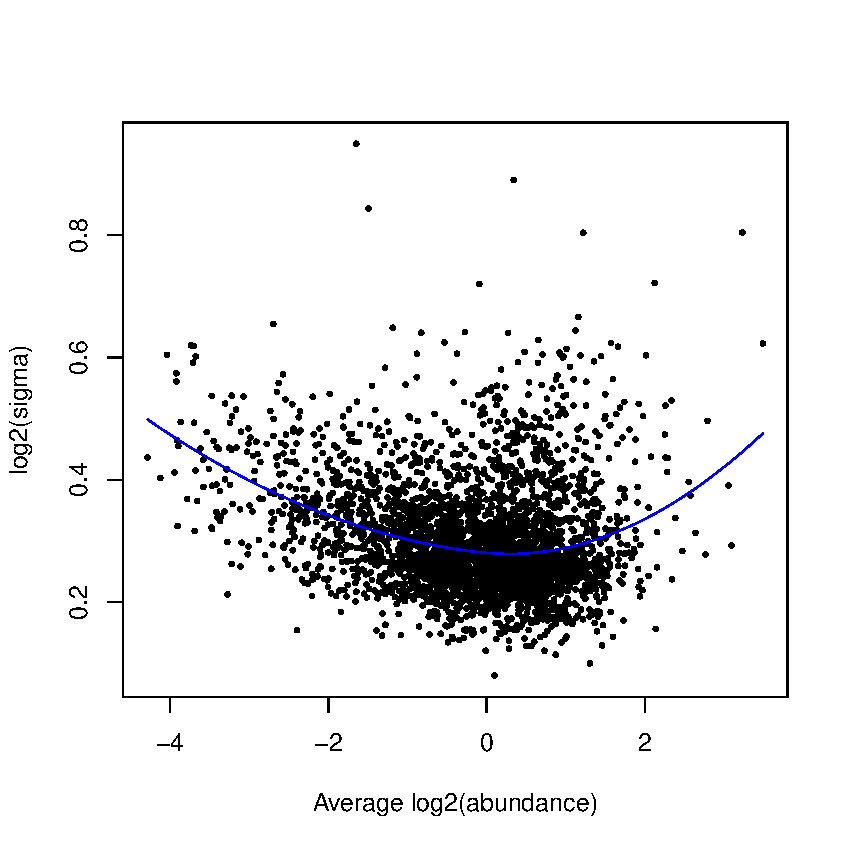
\includegraphics[height=0.3\textheight]{workflow_expressions_files/figure-latex/plotSA-1} \end{center}

The residual standard deviation is a measure of model accuracy and is most
easily conceptualized as a measurement of how far from the model prediction each
data point lies. The smaller the residual standard deviation, the closer the fit
between the model and observed data.

Next we will plot a p-value histogram. Importantly, this histogram shows the
distribution of p-values prior to any multiple hypothesis test correction or
false discovery rate control. This means plotting the \texttt{P.value} variable, not
the \texttt{adj.P.Val}.

\begin{Shaded}
\begin{Highlighting}[]
\DocumentationTok{\#\# Plot histogram of raw p{-}values}
\NormalTok{limma\_results }\SpecialCharTok{\%\textgreater{}\%}
  \FunctionTok{ggplot}\NormalTok{(}\FunctionTok{aes}\NormalTok{(}\AttributeTok{x =}\NormalTok{ P.Value)) }\SpecialCharTok{+}
  \FunctionTok{geom\_histogram}\NormalTok{(}\AttributeTok{binwidth =} \FloatTok{0.025}\NormalTok{) }\SpecialCharTok{+}
  \FunctionTok{labs}\NormalTok{(}\AttributeTok{x =} \StringTok{"P{-}value"}\NormalTok{, }\AttributeTok{y =} \StringTok{"Frequency"}\NormalTok{) }\SpecialCharTok{+}
  \FunctionTok{ggtitle}\NormalTok{(}\StringTok{"P{-}value distribution following Limma eBayes trend model"}\NormalTok{) }\SpecialCharTok{+}
  \FunctionTok{theme\_bw}\NormalTok{()}
\end{Highlighting}
\end{Shaded}

\begin{center}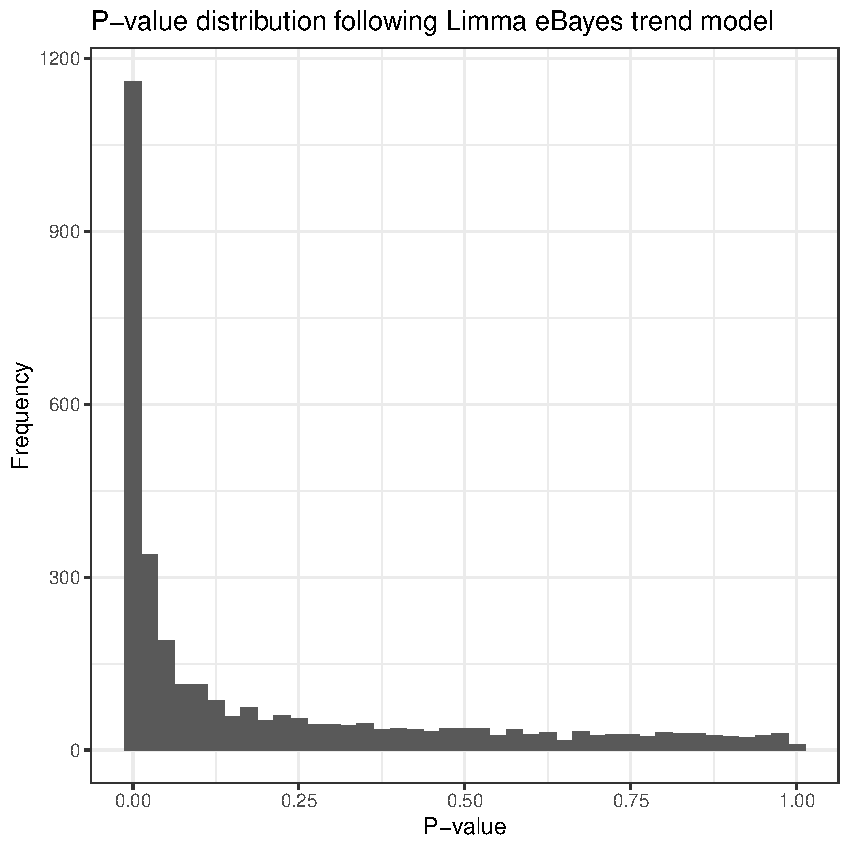
\includegraphics[height=0.3\textheight]{workflow_expressions_files/figure-latex/pvalue_histogram-1} \end{center}

The figure displayed shows an anti-conservative p-value distribution. The flat
distribution across the base of the graph represents the non-significant p-values
spread uniformly between 0 and 1, whilst the peak close to 0 contains significant
p-values, along with some false positives. For a more thorough explanation of
interpreting p-value distributions, including why your data may not produce an
anti-conservative distribution if your statistical model is inappropriate, please
see \citep{p_val}. Now, having applied the statistical model and verified it's
suitability, we take an initial look at the outputs.

\begin{Shaded}
\begin{Highlighting}[]
\DocumentationTok{\#\# Look at limma results table}
\FunctionTok{head}\NormalTok{(limma\_results)}
\end{Highlighting}
\end{Shaded}

\begin{verbatim}
## # A tibble: 6 x 8
##   Protein logFC AveExpr     t  P.Value  adj.P.Val     B TP   
##   <chr>   <dbl>   <dbl> <dbl>    <dbl>      <dbl> <dbl> <lgl>
## 1 Q01581   1.50   0.592  28.4 6.35e-10 0.00000205  13.1 FALSE
## 2 P15104   1.32   1.36   23.2 3.63e- 9 0.00000558  11.7 FALSE
## 3 Q9UK41   1.46  -1.49   21.7 6.36e- 9 0.00000558  11.2 FALSE
## 4 P37268   1.32  -0.674  21.0 8.58e- 9 0.00000558  10.9 FALSE
## 5 P04183   1.29   0.943  21.0 8.64e- 9 0.00000558  10.9 FALSE
## 6 Q9UHI8   2.45   0.368  18.8 2.21e- 8 0.0000119   10.0 FALSE
\end{verbatim}

The results table contains several important pieces of information. Each master
protein is represented by its accession number and has an associated log2 fold
change, that is the log2 difference in mean abundance between conditions, as
well as a log2 mean expression across all six samples, termed \texttt{AveExpr}. Since we
carried out an empirical Bayes moderated t-test, each protein also has a
moderated t-statistic and associated p-value. The moderated t-statistic can be
interpreted in the same way as a standard t-statistic. Each protein also has an
adjusted p-value which accounts for multiple hypothesis testing to control the
overall FDR. The default method for multiple hypothesis corrections within the
\texttt{topTable} function that we applied is the Benjamini and Hochberg (BH)
adjustment \citep{BH1995}, although we could have specified an alternative. Finally,
the B-statistic represents the log-odds that a protein is differentially abundant
between the two conditions, and the data is presented in descending order with
those with the highest log-odds of differential abundance at the top.

We can add annotations to this results table based on the user-defined
significance thresholds. In the literature, for stringent analyses a
FDR-adjusted p-value threshold of 0.01 is most frequently used, or 0.05 for
exploratory analyses. Ultimately these thresholds are arbitrary and set by the
user. The addition of a log-fold change (logFC) threshold is at the users
discretion and can be useful to determine significant results of biological
relevance. When using a TMT labelling strategy the co-isolation interference can
lead to substantial and uneven ratio compression, thus it is not recommended to
apply a fold change threshold here.

\begin{Shaded}
\begin{Highlighting}[]
\DocumentationTok{\#\# Add direction of log fold change relative to control}
\NormalTok{limma\_results}\SpecialCharTok{$}\NormalTok{direction }\OtherTok{\textless{}{-}} \FunctionTok{ifelse}\NormalTok{(limma\_results}\SpecialCharTok{$}\NormalTok{logFC }\SpecialCharTok{\textgreater{}} \DecValTok{0}\NormalTok{,}
                                  \StringTok{"up"}\NormalTok{, }\StringTok{"down"}\NormalTok{) }\SpecialCharTok{\%\textgreater{}\%}
  \FunctionTok{as.factor}\NormalTok{()}

\DocumentationTok{\#\# Add significance thresholds}
\NormalTok{limma\_results}\SpecialCharTok{$}\NormalTok{significance }\OtherTok{\textless{}{-}} \FunctionTok{ifelse}\NormalTok{(limma\_results}\SpecialCharTok{$}\NormalTok{adj.P.Val }\SpecialCharTok{\textless{}} \FloatTok{0.01}\NormalTok{,}
                                     \StringTok{"sig"}\NormalTok{, }\StringTok{"not.sig"}\NormalTok{) }\SpecialCharTok{\%\textgreater{}\%}
  \FunctionTok{as.factor}\NormalTok{()}


\DocumentationTok{\#\# Verify}
\FunctionTok{str}\NormalTok{(limma\_results)}
\end{Highlighting}
\end{Shaded}

\begin{verbatim}
## tibble [3,230 x 10] (S3: tbl_df/tbl/data.frame)
##  $ Protein     : chr [1:3230] "Q01581" "P15104" "Q9UK41" "P37268" ...
##  $ logFC       : num [1:3230] 1.5 1.32 1.46 1.32 1.29 ...
##  $ AveExpr     : num [1:3230] 0.592 1.363 -1.485 -0.674 0.943 ...
##  $ t           : num [1:3230] 28.4 23.2 21.7 21 21 ...
##  $ P.Value     : num [1:3230] 6.35e-10 3.63e-09 6.36e-09 8.58e-09 8.64e-09 ...
##  $ adj.P.Val   : num [1:3230] 2.05e-06 5.58e-06 5.58e-06 5.58e-06 5.58e-06 ...
##  $ B           : num [1:3230] 13.1 11.7 11.2 10.9 10.9 ...
##  $ TP          : logi [1:3230] FALSE FALSE FALSE FALSE FALSE FALSE ...
##  $ direction   : Factor w/ 2 levels "down","up": 2 2 2 2 2 2 1 2 1 2 ...
##  $ significance: Factor w/ 2 levels "not.sig","sig": 2 2 2 2 2 2 2 2 2 2 ...
\end{verbatim}

In the next code chunk, we use the \texttt{decideTests} function to determine how many
proteins are significantly up- and down- regulated in the treated compared to control
HEK293 cells. We tell this function to classify the significance of each
t-statistic based on a BH-adjusted p-value of 0.01. If we had not used TMT
labels and wished to include a logFC threshold, we could have included the \texttt{lfc} argument
and passed our desired logFC threshold. The function will then output a numerical
matrix containing either -1, 0, or 1 for each protein in each condition, where a
value of -1 indicates significant downregulation, 0 not significant and 1 significant
upregulation. To simplify interpretation, we print a \texttt{summary} of this matrix.

\begin{Shaded}
\begin{Highlighting}[]
\DocumentationTok{\#\# Get a summary of statistically significant results}
\NormalTok{fitted\_lm }\SpecialCharTok{\%\textgreater{}\%}
  \FunctionTok{decideTests}\NormalTok{(}\AttributeTok{adjust.method =} \StringTok{"BH"}\NormalTok{,}
              \AttributeTok{p.value =} \FloatTok{0.01}\NormalTok{) }\SpecialCharTok{\%\textgreater{}\%}
  \FunctionTok{summary}\NormalTok{()}
\end{Highlighting}
\end{Shaded}

\begin{verbatim}
##        (Intercept) cp_proteins$conditionTreated
## Down          1423                          381
## NotSig         404                         2536
## Up            1403                          313
\end{verbatim}

From this table we can see that 381 proteins were downregulated
in treated HEK293 cells compared to the control group whilst 313
were upregulated. Given that no logFC threshold was applied some of the significant
differences in abundance may be small. Further, these results mean little without
any information about which proteins these were and what roles they play within
the cell. We subset the significant proteins so that we can investigate them
further.

\begin{Shaded}
\begin{Highlighting}[]
\DocumentationTok{\#\# Subset proteins that show significantly different abundance}
\NormalTok{sig\_proteins }\OtherTok{\textless{}{-}} \FunctionTok{subset}\NormalTok{(limma\_results,}
\NormalTok{                       adj.P.Val }\SpecialCharTok{\textless{}=} \FloatTok{0.01}\NormalTok{)}

\FunctionTok{length}\NormalTok{(sig\_proteins}\SpecialCharTok{$}\NormalTok{Protein)}
\end{Highlighting}
\end{Shaded}

\begin{verbatim}
## [1] 694
\end{verbatim}

\subsection{Visualizing differentially abundant proteins}\label{visualizing-differentially-abundant-proteins}

Before looking deeper into which proteins have differential abundance, we first
create some simple plots to visualize the results. Volcano plots and MA plots
are two of the common visualisations used in this instance. When plotting the
former, users are advised to plot raw p-values rather than their derivative
BH-adjusted p-values. Point colours can be used to indicate significance based
on BH- adjusted p-values, as is shown in the code chunk below.

\begin{Shaded}
\begin{Highlighting}[]
\DocumentationTok{\#\# Generate a volcano plot}
\NormalTok{limma\_results }\SpecialCharTok{\%\textgreater{}\%}
  \FunctionTok{ggplot}\NormalTok{(}\FunctionTok{aes}\NormalTok{(}\AttributeTok{x =}\NormalTok{ logFC, }\AttributeTok{y =} \SpecialCharTok{{-}}\FunctionTok{log10}\NormalTok{(P.Value))) }\SpecialCharTok{+}
  \FunctionTok{geom\_point}\NormalTok{(}\FunctionTok{aes}\NormalTok{(}\AttributeTok{colour =}\NormalTok{ significance}\SpecialCharTok{:}\NormalTok{direction), }\AttributeTok{size =} \FloatTok{0.5}\NormalTok{) }\SpecialCharTok{+}
  \FunctionTok{scale\_color\_manual}\NormalTok{(}
    \AttributeTok{values =} \FunctionTok{c}\NormalTok{(}\StringTok{"black"}\NormalTok{, }\StringTok{"black"}\NormalTok{, }\StringTok{"deepskyblue"}\NormalTok{, }\StringTok{"red"}\NormalTok{), }\AttributeTok{name =} \StringTok{""}\NormalTok{,}
    \AttributeTok{labels =} \FunctionTok{c}\NormalTok{(}\StringTok{"Downregulated insignificant"}\NormalTok{,}
               \StringTok{"Upregulated insignificant"}\NormalTok{,}
               \StringTok{"Downregulated significant"}\NormalTok{,}
               \StringTok{"Upregulated significant"}\NormalTok{)) }\SpecialCharTok{+}
  \FunctionTok{theme}\NormalTok{(}\AttributeTok{axis.title.x =} \FunctionTok{element\_text}\NormalTok{(}\AttributeTok{size =} \DecValTok{15}\NormalTok{, }\AttributeTok{vjust =} \SpecialCharTok{{-}}\DecValTok{2}\NormalTok{),}
        \AttributeTok{axis.title.y =} \FunctionTok{element\_text}\NormalTok{(}\AttributeTok{size =} \DecValTok{15}\NormalTok{, }\AttributeTok{vjust =} \DecValTok{2}\NormalTok{),}
        \AttributeTok{axis.text.x =} \FunctionTok{element\_text}\NormalTok{(}\AttributeTok{size =} \DecValTok{12}\NormalTok{, }\AttributeTok{vjust =} \SpecialCharTok{{-}}\DecValTok{1}\NormalTok{),}
        \AttributeTok{axis.text.y =} \FunctionTok{element\_text}\NormalTok{(}\AttributeTok{size =} \DecValTok{12}\NormalTok{),}
        \AttributeTok{plot.background =} \FunctionTok{element\_rect}\NormalTok{(}\AttributeTok{fill =} \StringTok{"white"}\NormalTok{),}
        \AttributeTok{panel.background =} \FunctionTok{element\_rect}\NormalTok{(}\AttributeTok{fill =} \StringTok{"white"}\NormalTok{),}
        \AttributeTok{axis.line =} \FunctionTok{element\_line}\NormalTok{(}\AttributeTok{linewidth =} \FloatTok{0.5}\NormalTok{, }\AttributeTok{colour =} \StringTok{"black"}\NormalTok{),}
        \AttributeTok{plot.margin =} \FunctionTok{margin}\NormalTok{(}\DecValTok{10}\NormalTok{, }\DecValTok{10}\NormalTok{, }\DecValTok{10}\NormalTok{, }\DecValTok{10}\NormalTok{),}
        \AttributeTok{legend.position =} \FunctionTok{c}\NormalTok{(}\FloatTok{0.25}\NormalTok{, }\FloatTok{0.9}\NormalTok{)) }\SpecialCharTok{+}
  \FunctionTok{labs}\NormalTok{(}\AttributeTok{x =} \StringTok{"log2(FC)"}\NormalTok{, }\AttributeTok{y =} \StringTok{"{-}log10(p{-}value)"}\NormalTok{) }\SpecialCharTok{+}
  \FunctionTok{xlim}\NormalTok{(}\SpecialCharTok{{-}}\FloatTok{3.1}\NormalTok{, }\FloatTok{3.1}\NormalTok{)}
\end{Highlighting}
\end{Shaded}

\begin{verbatim}
## Warning: A numeric `legend.position` argument in `theme()` was deprecated in ggplot2
## 3.5.0.
## i Please use the `legend.position.inside` argument of `theme()` instead.
## This warning is displayed once every 8 hours.
## Call `lifecycle::last_lifecycle_warnings()` to see where this warning was
## generated.
\end{verbatim}

\begin{center}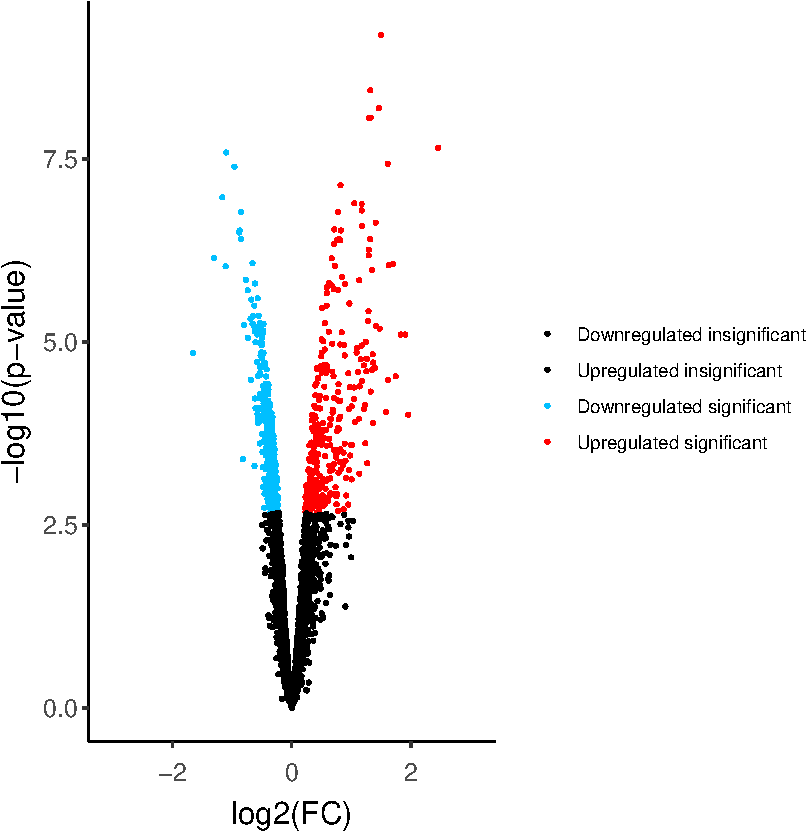
\includegraphics[height=0.4\textheight]{workflow_expressions_files/figure-latex/volcano_plot-1} \end{center}

\begin{Shaded}
\begin{Highlighting}[]
\DocumentationTok{\#\# Generate MA plot}
\NormalTok{limma\_results }\SpecialCharTok{\%\textgreater{}\%}
  \FunctionTok{ggplot}\NormalTok{(}\FunctionTok{aes}\NormalTok{(}\AttributeTok{x =}\NormalTok{ AveExpr, }\AttributeTok{y =}\NormalTok{ logFC)) }\SpecialCharTok{+}
  \FunctionTok{geom\_point}\NormalTok{(}\FunctionTok{aes}\NormalTok{(}\AttributeTok{colour =}\NormalTok{ significance}\SpecialCharTok{:}\NormalTok{direction), }\AttributeTok{size =} \FloatTok{0.5}\NormalTok{) }\SpecialCharTok{+}
  \FunctionTok{scale\_color\_manual}\NormalTok{(}
    \AttributeTok{values =} \FunctionTok{c}\NormalTok{(}\StringTok{"black"}\NormalTok{, }\StringTok{"black"}\NormalTok{, }\StringTok{"deepskyblue"}\NormalTok{, }\StringTok{"red"}\NormalTok{), }\AttributeTok{name =} \StringTok{""}\NormalTok{,}
    \AttributeTok{labels =} \FunctionTok{c}\NormalTok{(}\StringTok{"Downregulated insignificant"}\NormalTok{,}
               \StringTok{"Upregulated insignificant"}\NormalTok{,}
               \StringTok{"Downregulated significant"}\NormalTok{,}
               \StringTok{"Upregulated significant"}\NormalTok{)) }\SpecialCharTok{+}
  \FunctionTok{theme}\NormalTok{(}\AttributeTok{axis.title.x =} \FunctionTok{element\_text}\NormalTok{(}\AttributeTok{size =} \DecValTok{15}\NormalTok{, }\AttributeTok{vjust =} \SpecialCharTok{{-}}\DecValTok{2}\NormalTok{),}
        \AttributeTok{axis.title.y =} \FunctionTok{element\_text}\NormalTok{(}\AttributeTok{size =} \DecValTok{15}\NormalTok{, }\AttributeTok{vjust =} \DecValTok{2}\NormalTok{),}
        \AttributeTok{axis.text.x =} \FunctionTok{element\_text}\NormalTok{(}\AttributeTok{size =} \DecValTok{12}\NormalTok{, }\AttributeTok{vjust =} \SpecialCharTok{{-}}\DecValTok{1}\NormalTok{),}
        \AttributeTok{axis.text.y =} \FunctionTok{element\_text}\NormalTok{(}\AttributeTok{size =} \DecValTok{12}\NormalTok{),}
        \AttributeTok{plot.background =} \FunctionTok{element\_rect}\NormalTok{(}\AttributeTok{fill =} \StringTok{"white"}\NormalTok{),}
        \AttributeTok{panel.background =} \FunctionTok{element\_rect}\NormalTok{(}\AttributeTok{fill =} \StringTok{"white"}\NormalTok{),}
        \AttributeTok{axis.line =} \FunctionTok{element\_line}\NormalTok{(}\AttributeTok{linewidth =} \FloatTok{0.5}\NormalTok{, }\AttributeTok{colour =} \StringTok{"black"}\NormalTok{),}
        \AttributeTok{plot.margin =} \FunctionTok{margin}\NormalTok{(}\DecValTok{10}\NormalTok{, }\DecValTok{10}\NormalTok{, }\DecValTok{10}\NormalTok{, }\DecValTok{10}\NormalTok{),}
        \AttributeTok{legend.position =} \FunctionTok{c}\NormalTok{(}\FloatTok{0.25}\NormalTok{, }\FloatTok{0.9}\NormalTok{)) }\SpecialCharTok{+}
  \FunctionTok{xlab}\NormalTok{(}\StringTok{"log2(mean abundance)"}\NormalTok{) }\SpecialCharTok{+}
  \FunctionTok{ylab}\NormalTok{(}\StringTok{"log2(FC)"}\NormalTok{) }\SpecialCharTok{+}
  \FunctionTok{xlim}\NormalTok{(}\SpecialCharTok{{-}}\DecValTok{5}\NormalTok{, }\FloatTok{3.5}\NormalTok{)}
\end{Highlighting}
\end{Shaded}

\begin{center}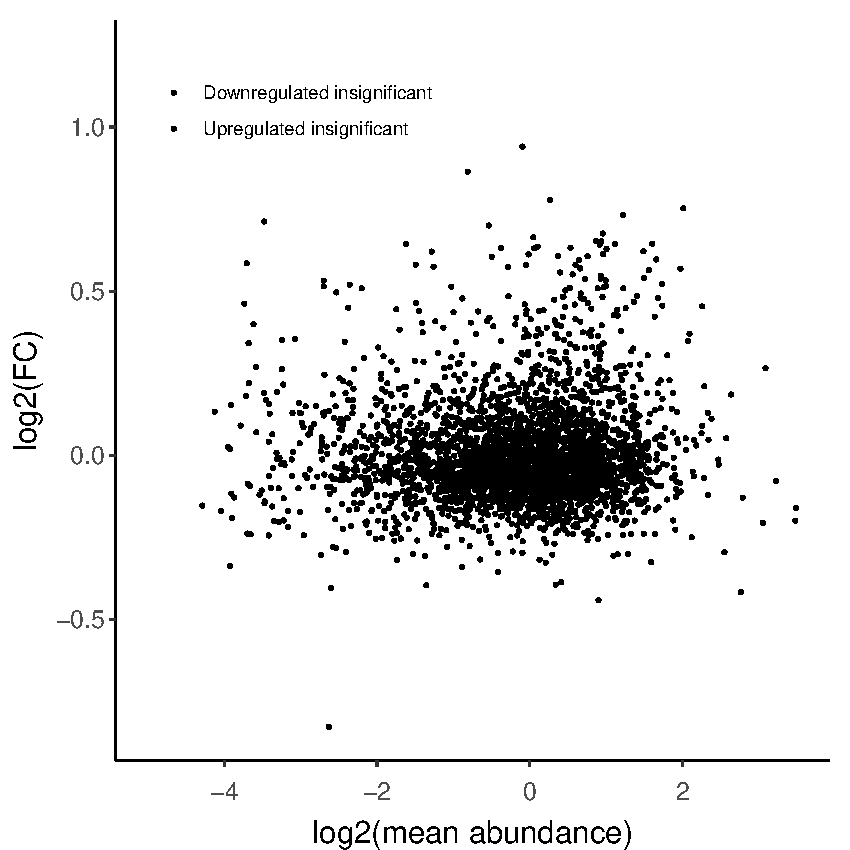
\includegraphics[height=0.4\textheight]{workflow_expressions_files/figure-latex/MA_plot-1} \end{center}

\subsection{Gene Ontology enrichment analysis}\label{gene-ontology-enrichment-analysis}

The final step in the processing workflow is to apply Gene Ontology (GO) enrichment
analyses to gain a biological understanding of the proteins which were either up
or downregulated in HEK293 cells upon treatment. GO terms provide descriptions
for genes and their corresponding proteins in the form of Molecular Functions
(MF), Biological Processes (BP) and Cellular Components (CC). By carrying out GO
enrichment analysis we can determine whether the frequency of any of these terms
is higher than expected in the proteins of interest compared to all of the proteins
which were detected. Such results can indicate whether proteins that were
increased or decreased in abundance in treated HEK293 cells represent particular
cellular locations, biological pathways or cellular functions.

Although GO enrichment analysis can be carried out online using websites such
as \href{http://cbl-gorilla.cs.technion.ac.il}{GOrilla} \citep{Eden2009} or
\href{http://www.pantherdb.org}{PantherDB} \citep{Mi2012, Thomas2021}, we advise against
this due to a lack of traceability and reproducibility. Instead, readers are
advised to make use of GO enrichment packages within the Bioconductor
infrastructure. Many such packages exist, including \href{https://bioconductor.org/packages/release/bioc/html/topGO.html}{\texttt{topGO}} \citep{topGO},
\href{https://www.bioconductor.org/packages/release/bioc/html/GOfuncR.html}{\texttt{GOfuncR}} \citep{GofuncR},
and \href{https://bioconductor.org/packages/release/bioc/html/clusterProfiler.html}{\texttt{clusterProfiler}}
\citep{Wu2021}. Here we will use \texttt{enrichGO} function in the \texttt{clusterProfiler} package.

First, we subset the accessions of proteins that we consider to be significantly
up or downregulated. These will be our proteins of interest.

\begin{Shaded}
\begin{Highlighting}[]
\DocumentationTok{\#\# Subset significantly upregulated and downregulated  proteins}
\NormalTok{sig\_up }\OtherTok{\textless{}{-}}\NormalTok{ limma\_results }\SpecialCharTok{\%\textgreater{}\%}
  \FunctionTok{filter}\NormalTok{(direction }\SpecialCharTok{==} \StringTok{"up"}\NormalTok{) }\SpecialCharTok{\%\textgreater{}\%}
  \FunctionTok{filter}\NormalTok{(significance }\SpecialCharTok{==} \StringTok{"sig"}\NormalTok{) }\SpecialCharTok{\%\textgreater{}\%}
  \FunctionTok{pull}\NormalTok{(Protein)}

\NormalTok{sig\_down }\OtherTok{\textless{}{-}}\NormalTok{ limma\_results }\SpecialCharTok{\%\textgreater{}\%}
  \FunctionTok{filter}\NormalTok{(direction }\SpecialCharTok{==} \StringTok{"down"}\NormalTok{) }\SpecialCharTok{\%\textgreater{}\%}
  \FunctionTok{filter}\NormalTok{(significance }\SpecialCharTok{==} \StringTok{"sig"}\NormalTok{) }\SpecialCharTok{\%\textgreater{}\%}
  \FunctionTok{pull}\NormalTok{(Protein)}
\end{Highlighting}
\end{Shaded}

Next, we input the UniProt IDs of up and downregulated proteins into the GO
enrichment analyses, as demonstrated below. Importantly, we provide the protein
list of interest as the foreground and a list of all proteins identified within
the study as the background, or `universe'. The \texttt{keyType} argument is used to
tell the function that our protein accessions are in UniProt format. This allows
mapping from UniProt ID back to a database containing the entire human genome
(\texttt{org.Hs.eg.db}). We also inform the function which GO categories we wish to
consider, here ``ALL'', meaning BP, MF and CC.

As well as the information outlined above, there is the opportunity for users to
specify various thresholds for statistical significance. These include
thresholds on original and adjusted p-values (using the \texttt{pvalueCutoff} argument)
as well as q-values (via the \texttt{qvalueCutoff} argument). Although many papers
often use `q- value' to mean `BH-adjusted p-value', the two are not always the
same and users should be explicit about the statistical thresholds that they
have applied. For exploratory purposes we will use the standard BH method for
FDR control and set p-value, BH-adjusted p-value, and q-value thresholds of
0.05.

\begin{Shaded}
\begin{Highlighting}[]
\DocumentationTok{\#\# Search for enriched GO terms within upregulated proteins}
\NormalTok{ego\_up }\OtherTok{\textless{}{-}} \FunctionTok{enrichGO}\NormalTok{(}\AttributeTok{gene =}\NormalTok{ sig\_up,}
                   \AttributeTok{universe =}\NormalTok{ limma\_results}\SpecialCharTok{$}\NormalTok{Protein,}
                   \AttributeTok{OrgDb =}\NormalTok{ org.Hs.eg.db,}
                   \AttributeTok{keyType =} \StringTok{"UNIPROT"}\NormalTok{,}
                   \AttributeTok{ont =} \StringTok{"ALL"}\NormalTok{,}
                   \AttributeTok{pAdjustMethod =} \StringTok{"BH"}\NormalTok{,}
                   \AttributeTok{pvalueCutoff =} \FloatTok{0.05}\NormalTok{,}
                   \AttributeTok{qvalueCutoff =} \FloatTok{0.05}\NormalTok{,}
                   \AttributeTok{readable =} \ConstantTok{TRUE}\NormalTok{)}

\DocumentationTok{\#\# Check results}
\NormalTok{ego\_up}
\end{Highlighting}
\end{Shaded}

\begin{verbatim}
## #
## # over-representation test
## #
## #...@organism     Homo sapiens 
## #...@ontology     GOALL 
## #...@keytype      UNIPROT 
## #...@gene     chr [1:313] "Q01581" "P15104" "Q9UK41" "P37268" "P04183" "Q9UHI8" "Q13907" ...
## #...pvalues adjusted by 'BH' with cutoff <0.05 
## #...2 enriched terms found
## 'data.frame':    2 obs. of  10 variables:
##  $ ONTOLOGY   : chr  "CC" "CC"
##  $ ID         : chr  "GO:0005758" "GO:0031970"
##  $ Description: chr  "mitochondrial intermembrane space" "organelle envelope lumen"
##  $ GeneRatio  : chr  "13/308" "13/308"
##  $ BgRatio    : chr  "40/3176" "44/3176"
##  $ pvalue     : num  5.59e-05 1.68e-04
##  $ p.adjust   : num  0.0208 0.0313
##  $ qvalue     : num  0.0207 0.0312
##  $ geneID     : chr  "CHCHD2/TIMM9/AK2/TIMM8B/COA4/COA6/MIX23/TIMM8A/DIABLO/TIMM13/TIMM10/TRIAP1/CYCS" "CHCHD2/TIMM9/AK2/TIMM8B/COA4/COA6/MIX23/TIMM8A/DIABLO/TIMM13/TIMM10/TRIAP1/CYCS"
##  $ Count      : int  13 13
## #...Citation
##  T Wu, E Hu, S Xu, M Chen, P Guo, Z Dai, T Feng, L Zhou, W Tang, L Zhan, X Fu, S Liu, X Bo, and G Yu.
##  clusterProfiler 4.0: A universal enrichment tool for interpreting omics data.
##  The Innovation. 2021, 2(3):100141
\end{verbatim}

We can see from the results that there are 2 significantly
enriched terms associated with the upregulated proteins. Next, we take a look at
the downregulated proteins.

\begin{Shaded}
\begin{Highlighting}[]
\DocumentationTok{\#\# Search for enriched GO terms within downregulated proteins}
\NormalTok{ego\_down }\OtherTok{\textless{}{-}} \FunctionTok{enrichGO}\NormalTok{(}\AttributeTok{gene =}\NormalTok{ sig\_down,}
                     \AttributeTok{universe =}\NormalTok{ limma\_results}\SpecialCharTok{$}\NormalTok{Protein,}
                     \AttributeTok{OrgDb =}\NormalTok{ org.Hs.eg.db,}
                     \AttributeTok{keyType =} \StringTok{"UNIPROT"}\NormalTok{,}
                     \AttributeTok{ont =} \StringTok{"ALL"}\NormalTok{,}
                     \AttributeTok{pAdjustMethod =} \StringTok{"BH"}\NormalTok{,}
                     \AttributeTok{pvalueCutoff =} \FloatTok{0.05}\NormalTok{,}
                     \AttributeTok{qvalueCutoff =} \FloatTok{0.05}\NormalTok{,}
                     \AttributeTok{readable =} \ConstantTok{TRUE}\NormalTok{)}

\DocumentationTok{\#\# Check results}
\NormalTok{ego\_down}
\end{Highlighting}
\end{Shaded}

\begin{verbatim}
## #
## # over-representation test
## #
## #...@organism     Homo sapiens 
## #...@ontology     GOALL 
## #...@keytype      UNIPROT 
## #...@gene     chr [1:381] "Q53EL6" "P08243" "P35716" "Q92878" "P26583" "Q92522" "O43657" ...
## #...pvalues adjusted by 'BH' with cutoff <0.05 
## #...61 enriched terms found
## 'data.frame':    61 obs. of  10 variables:
##  $ ONTOLOGY   : chr  "BP" "BP" "BP" "BP" ...
##  $ ID         : chr  "GO:0006310" "GO:0000725" "GO:0006302" "GO:0006520" ...
##  $ Description: chr  "DNA recombination" "recombinational repair" "double-strand break repair" "amino acid metabolic process" ...
##  $ GeneRatio  : chr  "37/366" "23/366" "32/366" "33/366" ...
##  $ BgRatio    : chr  "95/3121" "58/3121" "101/3121" "113/3121" ...
##  $ pvalue     : num  3.61e-12 3.61e-08 4.54e-08 2.48e-07 4.46e-07 ...
##  $ p.adjust   : num  8.65e-09 3.62e-05 3.62e-05 1.48e-04 2.14e-04 ...
##  $ qvalue     : num  8.33e-09 3.48e-05 3.48e-05 1.43e-04 2.06e-04 ...
##  $ geneID     : chr  "RAD50/HMGB2/H1-10/RADX/MRE11/H1-0/H1-2/ZMYND8/MCM5/HMGB3/NUCKS1/RAD21/PRKDC/SFPQ/MCM4/XRCC6/HTATSF1/H1-3/MCM7/T"| __truncated__ "RADX/MRE11/ZMYND8/MCM5/NUCKS1/RAD21/SFPQ/MCM4/XRCC6/HTATSF1/MCM7/XRCC5/PPP4R2/POGZ/YY1/MCM3/MCM2/VPS72/PARP1/BR"| __truncated__ "RAD50/HMGB2/RADX/MRE11/DEK/ZMYND8/MCM5/NUCKS1/RAD21/PRKDC/TP53/SMARCC2/SFPQ/MCM4/XRCC6/HPF1/HTATSF1/MCM7/XRCC5/"| __truncated__ "ASNS/PHGDH/SDSL/SARS1/YARS1/AARS2/HMGCL/GARS1/IARS2/AARS1/HIBADH/PYCR1/ACADSB/DHFR/MCCC2/SLC25A12/MARS1/PSAT1/S"| __truncated__ ...
##  $ Count      : int  37 23 32 33 21 14 55 14 14 44 ...
## #...Citation
##  T Wu, E Hu, S Xu, M Chen, P Guo, Z Dai, T Feng, L Zhou, W Tang, L Zhan, X Fu, S Liu, X Bo, and G Yu.
##  clusterProfiler 4.0: A universal enrichment tool for interpreting omics data.
##  The Innovation. 2021, 2(3):100141
\end{verbatim}

The downregulated proteins contain 61 significantly enriched GO
terms. There are many ways in which users can represent these results visually.
Here, we create a barplot using the \texttt{barplot} function from the \href{https://bioconductor.org/packages/release/bioc/html/enrichplot.html}{\texttt{enrichplot} package}
\citep{enrichplot}. Users are directed to the vignette of the \texttt{enrichplot} package
for additional visualization options and guidance. We plot the first 10 GO terms
i.e.~the 10 GO terms with the greatest enrichment.

\begin{Shaded}
\begin{Highlighting}[]
\DocumentationTok{\#\# Plot the results}
\FunctionTok{barplot}\NormalTok{(ego\_down,}
        \AttributeTok{x =} \StringTok{"Count"}\NormalTok{,}
        \AttributeTok{showCategory =} \DecValTok{10}\NormalTok{,}
        \AttributeTok{font.size =} \DecValTok{12}\NormalTok{,}
        \AttributeTok{label\_format =} \DecValTok{28}\NormalTok{,}
        \AttributeTok{colorBy =} \StringTok{"p.adjust"}\NormalTok{)}
\end{Highlighting}
\end{Shaded}

\begin{center}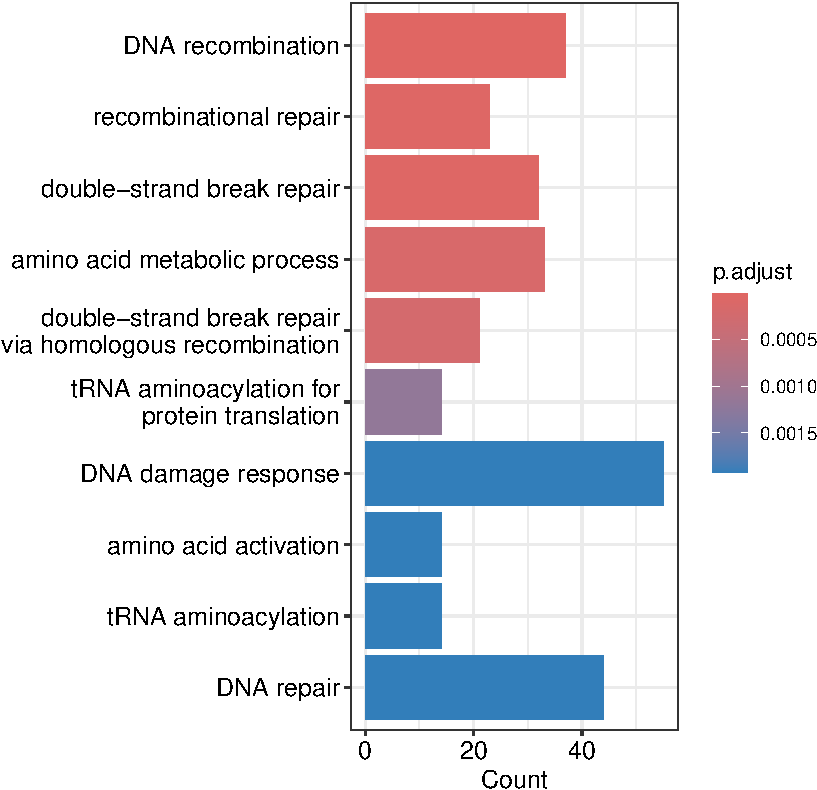
\includegraphics[height=0.4\textheight]{workflow_expressions_files/figure-latex/GO_enrichment_plot-1} \end{center}

\section{Writing and exporting data}\label{writing-and-exporting-data}

Finally, we export the results of our statistical analyses as \texttt{.csv} files.

\begin{Shaded}
\begin{Highlighting}[]
\DocumentationTok{\#\# Save results of Limma statistics}
\FunctionTok{write.csv}\NormalTok{(gene\_results, }\AttributeTok{file =} \StringTok{"all\_limma\_results.csv"}\NormalTok{)}

\DocumentationTok{\#\# Save subsets of upregulated and downregulated proteins}
\FunctionTok{write.csv}\NormalTok{(sig\_upregulated, }\AttributeTok{file =} \StringTok{"upregulated\_results.csv"}\NormalTok{)}
\FunctionTok{write.csv}\NormalTok{(sig\_downregulated, }\AttributeTok{file =} \StringTok{"downregulated\_results.csv"}\NormalTok{)}\ErrorTok{)}

\DocumentationTok{\#\# Save results of GO enrichment}
\FunctionTok{write.csv}\NormalTok{(ego\_up, }\AttributeTok{file =} \StringTok{"upregulated\_go\_enrichment.csv"}\NormalTok{)}
\FunctionTok{write.csv}\NormalTok{(ego\_down, }\AttributeTok{file =} \StringTok{"downregulated\_go\_enrichment.csv"}\NormalTok{)}
\end{Highlighting}
\end{Shaded}

Users can also use the \href{https://www.rdocumentation.org/packages/ggplot2/versions/0.9.0/topics/ggsave}{\texttt{ggsave}}
function to export any of the figures generated.

\section{Discussion and conclusion}\label{discussion-and-conclusion}

Expression proteomics is becoming an increasingly important tool in modern
molecular biology. As more researchers participate in expression proteomics,
either by collecting data or accessing data collected by others, there is a need
for clear illustration(s) of how to deal with such complex data.

Existing bottom-up proteomics workflows for differential expression analysis
either provide pipelines with limited user control and flexibility (e.g., \texttt{MSstats}
and \texttt{MSstatsTMT} \citep{Choi2014, Huang2020}), can only be applied to specific data
formats (e.g., \texttt{Proteus} which is limited to input from MaxQuant \citep{Gierlinski2018}),
or provide very limited commentary. The latter directly contributes to a
problematic disconnect between researchers and their data whereby the users do
not understand if or why each step is necessary for their given dataset and
biological question. This can prevent researchers from refining a workflow to fit
their specific needs. Finally, the majority of proteomics workflows utilize
\texttt{data.frame} or \texttt{tibble} structures which limits their traceability, as is the
case for \texttt{protti}, \texttt{promor} and \texttt{prolfqua} \citep{Ranathunge2022, Quast2021, Wolski2022}.

The workflow presented here outlines in completion how to process, analyze and
interpret LFQ and TMT expression proteomics data derived from a bottom-up DDA
experiment. Critically, we emphasize quality control and data-guided decisions
with an extensive explanation of all key steps and how they may differ in
various scenarios (e.g., the quantitation method, instrumentation and biological
question). Our workflow takes advantage of the relatively recent \texttt{QFeatures}
infrastructure to ensure explicit and transparent data pre-processing as well as
to provide an easy way for users to trace back through their analyses. These
features are particularly important for beginners who wish to gain a better
understanding of their data and how it changes throughout this workflow.

No single workflow can demonstrate the processing, analysis and interpretation
of all proteomics data. Our workflow is currently suitable for DDA datasets with
label-free or TMT-based quantitation. We do not include examples of experiments
that combine data from multiple TMTplexes, although the code provided could
easily be expanded to include such a scenario. This workflow provides an in-depth
user-friendly pipeline for both new and experienced proteomics data analysts.

\section{Session information and getting help}\label{session-information-and-getting-help}

The workflows provided involve use of functions from many different
R/Bioconductor packages. The \texttt{sessionInfo} function provides an easy way to
summarize all packages and the corresponding versions used to generate this
document. Should software updates lead to the generation of errors or different
results to those demonstrated here, such changes should be easily traced.

\begin{Shaded}
\begin{Highlighting}[]
\DocumentationTok{\#\# Print session information}
\FunctionTok{sessionInfo}\NormalTok{()}
\end{Highlighting}
\end{Shaded}

\begin{verbatim}
## R version 4.4.0 (2024-04-24)
## Platform: aarch64-apple-darwin20
## Running under: macOS Ventura 13.2
## 
## Matrix products: default
## BLAS:   /Library/Frameworks/R.framework/Versions/4.4-arm64/Resources/lib/libRblas.0.dylib 
## LAPACK: /Library/Frameworks/R.framework/Versions/4.4-arm64/Resources/lib/libRlapack.dylib;  LAPACK version 3.12.0
## 
## locale:
## [1] en_US.UTF-8/en_US.UTF-8/en_US.UTF-8/C/en_US.UTF-8/en_US.UTF-8
## 
## time zone: Europe/London
## tzcode source: internal
## 
## attached base packages:
## [1] stats4    stats     graphics  grDevices utils     datasets  methods  
## [8] base     
## 
## other attached packages:
##  [1] patchwork_1.2.0             enrichplot_1.24.0          
##  [3] clusterProfiler_4.12.0      org.Hs.eg.db_3.19.1        
##  [5] AnnotationDbi_1.66.0        limma_3.60.0               
##  [7] Biostrings_2.72.0           XVector_0.44.0             
##  [9] corrplot_0.92               NormalyzerDE_1.22.0        
## [11] tibble_3.2.1                dplyr_1.1.4                
## [13] stringr_1.5.1               ggplot2_3.5.1              
## [15] QFeatures_1.14.0            MultiAssayExperiment_1.30.1
## [17] SummarizedExperiment_1.34.0 Biobase_2.64.0             
## [19] GenomicRanges_1.56.0        GenomeInfoDb_1.40.0        
## [21] IRanges_2.38.0              S4Vectors_0.42.0           
## [23] BiocGenerics_0.50.0         MatrixGenerics_1.16.0      
## [25] matrixStats_1.3.0          
## 
## loaded via a namespace (and not attached):
##   [1] RColorBrewer_1.1-3       rstudioapi_0.16.0        jsonlite_1.8.8          
##   [4] magrittr_2.0.3           farver_2.1.1             rmarkdown_2.26          
##   [7] fs_1.6.4                 zlibbioc_1.50.0          vctrs_0.6.5             
##  [10] memoise_2.0.1            ggtree_3.12.0            tinytex_0.51            
##  [13] BiocBaseUtils_1.6.0      htmltools_0.5.8.1        S4Arrays_1.4.0          
##  [16] usethis_2.2.3            gridGraphics_0.5-1       SparseArray_1.4.3       
##  [19] plyr_1.8.9               impute_1.78.0            cachem_1.0.8            
##  [22] igraph_2.0.3             lifecycle_1.0.4          pkgconfig_2.0.3         
##  [25] gson_0.1.0               Matrix_1.7-0             R6_2.5.1                
##  [28] fastmap_1.1.1            GenomeInfoDbData_1.2.12  clue_0.3-65             
##  [31] digest_0.6.35            aplot_0.2.2              colorspace_2.1-0        
##  [34] RSQLite_2.3.6            labeling_0.4.3           fansi_1.0.6             
##  [37] httr_1.4.7               polyclip_1.10-6          abind_1.4-5             
##  [40] compiler_4.4.0           bit64_4.0.5              withr_3.0.0             
##  [43] BiocParallel_1.38.0      viridis_0.6.5            DBI_1.2.2               
##  [46] ggforce_0.4.2            MASS_7.3-60.2            DelayedArray_0.30.1     
##  [49] HDO.db_0.99.1            tools_4.4.0              scatterpie_0.2.2        
##  [52] ape_5.8                  glue_1.7.0               nlme_3.1-164            
##  [55] GOSemSim_2.30.0          shadowtext_0.1.3         grid_4.4.0              
##  [58] cluster_2.1.6            reshape2_1.4.4           fgsea_1.30.0            
##  [61] generics_0.1.3           gtable_0.3.5             preprocessCore_1.66.0   
##  [64] tidyr_1.3.1              data.table_1.15.4        tidygraph_1.3.1         
##  [67] utf8_1.2.4               ggrepel_0.9.5            pillar_1.9.0            
##  [70] yulab.utils_0.1.4        BiocWorkflowTools_1.30.0 splines_4.4.0           
##  [73] tweenr_2.0.3             treeio_1.28.0            lattice_0.22-6          
##  [76] bit_4.0.5                tidyselect_1.2.1         GO.db_3.19.1            
##  [79] knitr_1.46               git2r_0.33.0             gridExtra_2.3           
##  [82] bookdown_0.39            ProtGenerics_1.36.0      xfun_0.43               
##  [85] graphlayouts_1.1.1       statmod_1.5.0            stringi_1.8.4           
##  [88] UCSC.utils_1.0.0         lazyeval_0.2.2           ggfun_0.1.4             
##  [91] yaml_2.3.8               evaluate_0.23            codetools_0.2-20        
##  [94] ggraph_2.2.1             MsCoreUtils_1.16.0       qvalue_2.36.0           
##  [97] BiocManager_1.30.23      ggplotify_0.1.2          cli_3.6.2               
## [100] munsell_0.5.1            Rcpp_1.0.12              png_0.1-8               
## [103] parallel_4.4.0           blob_1.2.4               DOSE_3.30.0             
## [106] AnnotationFilter_1.28.0  tidytree_0.4.6           viridisLite_0.4.2       
## [109] scales_1.3.0             purrr_1.0.2              crayon_1.5.2            
## [112] rlang_1.1.3              cowplot_1.1.3            fastmatch_1.1-4         
## [115] KEGGREST_1.44.0
\end{verbatim}

Users are advised to update R itself as well as packages as required.
Bioconductor packages can be updated using the \texttt{BiocManager::install()}
function, as shown below.

\begin{Shaded}
\begin{Highlighting}[]
\ControlFlowTok{if}\NormalTok{ (}\SpecialCharTok{!}\FunctionTok{require}\NormalTok{(}\StringTok{"BiocManager"}\NormalTok{, }\AttributeTok{quietly =} \ConstantTok{TRUE}\NormalTok{)) \{}
  \FunctionTok{install.packages}\NormalTok{(}\StringTok{"BiocManager"}\NormalTok{)}
\NormalTok{\}}
\NormalTok{BiocManager}\SpecialCharTok{::}\FunctionTok{install}\NormalTok{()}
\end{Highlighting}
\end{Shaded}

\section{Data availability}\label{data-availability}

This workflow is written in the R statistical programming language and uses
freely available open-source software packages from \href{https://cran.r-project.org}{CRAN}
and \href{https://bioconductor.org}{Bioconductor}. Version numbers for all packages
are shown in the Session information section.

Raw mass spectrometry data is freely available online through the
ProteomeXchange Consortium via the PRIDE repository with identifier PXD041794.
All processed data is available at
\url{http://doi.org/10.5281/zenodo.11196770},
and at GitHub repository \url{https://github.com/CambridgeCentreForProteomics/f1000_expression_proteomics}.

\section{Author contributions}\label{author-contributions}

C. H. conceptualization, investigation, methodology, project administration,
software, validation, writing -- original draft preparation, review and editing;
C. S. D. software and writing - review and editing; T. K. methodology,
supervision, software, writing - review and editing; K. S. L. funding acquisition,
supervision, writing - review and editing; L. M. B. conceptualization, methodology,
supervision, writing - review and editing.

\section{Competing interests}\label{competing-interests}

No competing interests were disclosed.

\section{Grant information}\label{grant-information}

C. H. is funded through a BBSRC CASE award with AstraZeneca (BB/W509929/1). C. S.
D. is funded by a Herchel Smith Research Studentship at the University of
Cambridge, United Kingdom. T. K. is funded by a Gordon and Betty Moore Foundation
Grant (\#7872). K. S. L. is funded by Wellcome Trust (110071/Z/15/Z) and European
Union Horizon 2020 program INFRAIA project EPIC-XS (project no.: 823839). L. M.
B. is funded by European Union Horizon 2020 program INFRAIA project EPIC-XS
(project no.: 823839).

The funders had no role in study design, data collection and analysis, decision
to publish, or preparation of the manuscript.

\section{Acknowledgements}\label{acknowledgements}

The authors would like to thank Savvas Kourtis from the Centre for Genomic
Regulation, Barcelona, and Oliver M. Crook, from the Department of Statistics,
Oxford University, UK, for trialing this workflow.

\section{Appendix}\label{appendix}

\subsection{Identification search with Proteome Discoverer}\label{identification-search-with-proteome-discoverer}

The use-case data analyzed in this workflow was initially processed using
\href{https://www.thermofisher.com/uk/en/home/industrial/mass-spectrometry/liquid-chromatography-mass-spectrometry-lc-ms/lc-ms-software/multi-omics-data-analysis/proteome-discoverer-software.html}{Proteome Discoverer}
version 2.5. Whilst much of the identification and quantification takes place
out of sight of the user, Proteome Discoverer incorporates several user-defined
search parameters which must be specified according to the sample preparation
methods and MS instrumentation used. There is also the option to apply both
basic and advanced data filtering parameters during the search. Users must be
aware of these parameters as they will directly influence the data output and
downstream processing.

Whilst an in-depth discussion of identification searches is outside of the scope
of this workflow, a few key parameters are discussed to put the data into
context. During sample preparation, TMT-labelled cell pellets were combined and
separated into 8 fractions using a Pierce High pH Reversed-Phase Peptide
Fractionation Kit (Thermo Fisher Scientific). After being analyzed by MS, the 8
resulting raw files were uploaded to Proteome Discoverer 2.5 and processed using
a single processing and consensus workflow. LFQ supernatant fractions were each
analyzed on a separate mass spectrometry run resulting in 6 raw files. These
files were imported into Proteome Discoverer with each sample having its own
independent processing step followed by a single multi-consensus step. All
processing and consensus workflow templates are provided in the supplementary
materials.

For both TMT and LFQ workflows, SequestHT was selected as the search engine and
trypsin specified as the enzyme used for proteolytic digestion. Since the
digestion was carried out overnight with a 1:20 w/w ratio of trypsin:protein,
digestion was expected to be complete and a low threshold of 2 missed cleavages
was allowed. For MS analysis, a Fourier Transform orbitrap with a resolving
power of 120,000 m/z was used as the mass analyzer for precursor ion mass, and a
linear ion trap was used to measure fragment ion mass. This information
determined the thresholds for precursor and fragment mass tolerances, two key
parameters for the identification search. The precursor mass tolerance
determines which mass range of peptide sequences are considered for each
observed spectrum, whilst the fragment mass tolerance specifies how similar the
observed and theoretical peptide fragment spectra should be for a match. If
these tolerances are too narrow then the correct peptide sequence may be omitted
and true positives are lost. However, if thresholds are set too wide then
incorrect peptide sequences are considered and false positives arise. Based on
the instrumentation used in this experiment, standard mass tolerances of 10 ppm
and 0.5 Da were allowed for precursors and fragments, respectively. Given the
intrinsic variability of LFQ between MS runs, RT alignment was used for the
label-free samples with a 10-minute retention time window.

In addition to the parameters based on the experimental protocol, we also
applied some basic non-specific filtering. We only retained high confidence PSMs
from the identification search. Such filtering is necessary because only a
fraction of the PSMs outputted by any given search engine will be genuine
matches, or true discoveries, whilst the remainder are incorrect false
discoveries. To deal with this problem, PSM confidence level (high, medium or
low) is determined via the Proteome Discoverer Percolator node \citep{Kll2007} which
estimates each PSM's false discovery rate (FDR). The raw spectra are searched
against the database of interest as well as a decoy database containing
randomised peptide sequences, often generated by shuffling or reversing the
original peptide sequences. False discovery rate is then defined as the
proportion of total PSMs that are matched to the decoy database, and, therefore,
are known false discoveries. This is done for all spectra and we considered a
PSM to be of `high confidence' if it had a false discovery rate \textless1 \%, `medium
confidence' if \textless5 \%, and `low confidence' if the false discovery rate exceeded
5 \%. Only PSMs annotated as high confidence were kept.

Whilst the basic filtering steps completed during this identification search
could just have easily been carried out in R using the \texttt{SummarizedExperiment}
and \texttt{QFeatures} infrastructure, applying them here saves time later on and
reduces the burden of storing large data files. These steps are also relatively
standard and non-specific so we do not need to assess the data prior to their
implementation. However, Proteome Discoverer also provides the option to carry
out more in-depth filtering through the use of parameters such as the SPS Mass
Match \%, co-isolation interference \% and signal-to-noise thresholds. We advise
against implementing such filtering at this stage since decisions regarding
thresholds will likely be influenced by the quality of data output, as
demonstrated later in this workflow. Instead, thresholds for the three
aforementioned parameters were set to 0 during the identification search.

{\small\bibliography{refs.bib}}

\end{document}
